\documentclass[a4paper,10pt]{scrartcl}
\usepackage{etex}
\usepackage{mathe-vorlesung}
\usepackage{graphicx}
\usepackage[all]{xy}
\renewcommand{\equiv}{\Longleftrightarrow}
\newcommand{\eps}{\varepsilon}
\newcommand{\del}{\delta}
\newcommand{\homo}{\cong}
\usepackage{txfonts}
\renewcommand{\bigsqcap}{\prod}
\usepackage{tikz}
\usetikzlibrary{arrows,patterns,matrix}
\usetikzlibrary{shapes.geometric}
\usetikzlibrary{decorations.markings}
\usepackage{float}
\usepackage[T1]{fontenc}
\usepackage{stmaryrd}

\title{Topologie}

\begin{document}

\maketitle

\tableofcontents
\newpage
\begin{center}
\LARGE\textbf{Vorwort}
\end{center}
\begin{seg}{Was ist Topologie?}
\begin{itemize}
\item "` Untersuchung geometrischer Objekte bis auf stetige Deformationen. "'
\item "` Stetigkeitsgeometrie"', "` qualitative Geometrie "', "`Gummi-Geometrie"'
\end{itemize}
Objekte werden in der Topologie als gleich angesehen, wenn sie durch eine in beiden Richtungen stetige bijektive Abbildung aufeinander abgebildet werden kann ("` Homöomorphismus"').
\end{seg}
So zum Beispiel für Teilmengen des $\R^2$:
\begin{figure}[h]
\centering
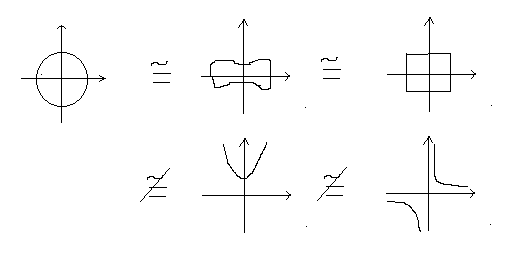
\includegraphics[scale=0.7]{fig1.png}
\caption{}
\end{figure}
\begin{ex*}
\begin{figure}[H]
 \centering
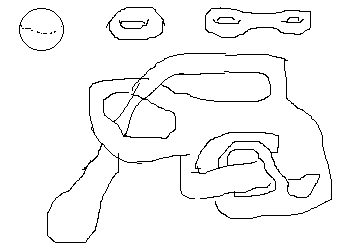
\includegraphics[scale=0.7]{fig2.png}
\caption{}
\end{figure}
Topologische Begriffe sind beispielsweise \emph{Stetigkeit, offene/ abgeschlossene Mengen, Umgebung, Rand, Abschluss, Konvergenz, kompakt, zusammenhängend, Homotopie}.  Die konkreten Definitionen werden im Verlauf dieser Vorlesung geklärt.
\end{ex*}
\section{Grundbegriffe}
\subsection{Metrische und topologische Räume}
\begin{df}
Ein \emph{metrischer Raum} ist eine Menge $X$ zusammen mit einer Funktion $d: X \times X \rightarrow \R$, genannt \emph{Metrik} oder \emph{Abstandsfunktion}, so dass folgende Axiome gelten:
\begin{enumerate}[(\roman{enumi})]
\item \emph{Positivität}: $d(x,y)\ge 0 \land d(x,y)=0\equiv x=y$
\item \emph{Symmetrie}: $d(x,y)=d(y,x)$
\item \emph{Dreiecksungleichung}: $d(x,z) \le d(x,y)+d(y,z)$
\end{enumerate}
\end{df}
\begin{ex*}
Auf $\R^n$ ist durch die \emph{Euklidische Norm} $||x||=\sqrt{x_1^2+\dotsb +x_n^2}$ die \emph{Euklidische Abstandsfunktion} $d(x,y)=||x-y||$ gegeben. Auf $\R$ oder auf $\C$ ist diese Metrik durch den Betrag $d(x,y):=|x-y|$ definiert.  Man erhält auf diese Weise aus jeder Norm eine Metrik. Hierbei liefern verschiedene Normen natürlich verschiedene Metriken. Hier einige Beispiele auf $\R^2$:
\begin{itemize} 
\item euklidische Norm: $||x||_2=\sqrt{x_1^2+x_2^2}$
\item Maximumsnorm: $||x||_\infty := \max(|x_1|, |x_2|)$
\item $\Eins$-Norm $||x||_1 := |x_1|+|x_2|$
\end{itemize}
\end{ex*}

\begin{ex*}
Die diskrete Metrik definiert durch:
\[
d(x,y)=\begin{cases}
  0, & \text{falls } x=y \\ 1, & \text{falls } x\neq y
\end{cases}
\]
\end{ex*}

Es lassen sich zwei zentrale mathematische Begriffe mit Hilfe von Abstandsfunktionen definieren:
\begin{itemize}
\item Konvergenz von Folgen
\item Stetigkeit von Abbildungen
\end{itemize}

\begin{df}[Konvergenz im metrischen Räumen]
Sei $X$ ein metrischer Raum und $x_n, n\in \N$ eine Folge in $X$. Wir sagen $(x_n)_{n\in \N}$ \emph{konvergiert}, falls es ein $a \in X$ gibt, so dass gilt:
\[
\forall_{\varepsilon>0}\exists_{k\in\N}\forall_{n\ge k}: d(x_n,a)<\varepsilon
\]
\end{df}
In diesem Fall sagen wir, $a$ ist der \emph{Limes} (oder Grenzwert) von $(x_n)_{n\in \N}$ (und schreiben $x_n\rightarrow a, \lim\limits_{n\rightarrow \infty} x_n=a$) 

\begin{st} 
In einem metrischen Raum ist der Limes eine konvergente Folge eindeutig bestimmt.
\end{st}
\begin{proof}
Seien $a$ und $b$ Limiten von $(x_n)_{n\in \N}$ mit $\delta := d(a,b)>0$.

Da $(x_n)_{n\in \N}$ gegen $a$ konvergiert, gibt es $k\in \N$, sodass $d(x_n,a)<\frac{\delta}{2}$ für alle $n \ge k$.
Dann gilt nach Dreiecksungleichung:
\[
\delta=d(a,b)\le \underbrace{d(a,x_n)}_{<\frac{\delta}{2}}+d(x_n,b)
\]
Also gilt $d(x_n,b)\ge \frac{\delta}{2}$ für alle $n\ge k$, was der Konvergenz gegen $b$ widerspricht.
\end{proof}
\begin{df}[$\eps$-$\delta$-Definition der Stetigkeit in metrischen Räumen]
Seien $X$ und $\tilde X$ metrische Räume mit Abstandsfunktion $d$ bzw. $\tilde d$. Eine Abbildung $f: X \rightarrow \tilde X$ heißt stetig in $x \in X$ falls gilt: 
\[\forall_{\eps>0}\exists_{\delta>0} \forall_{x'\in X}: d(x,x')<\delta \implies \tilde d(f(x), f(x'))<\eps\]

Die Abbildung heißt \emph{stetig}, falls dies für alle $x\in X$ gilt.  
\end{df}
Stetigkeit in metrischen Räumen hängen eng zusammen. Es gilt:
\begin{st}
Eine Abbildung $f: X\rightarrow \tilde X$ zwischen metrischen Räume ist genau dann stetig, wenn für jede konvergente Folge $x_n \rightarrow a$ in X gilt, dass $f(x_n) \rightarrow f(a)$
\end{st} 
\begin{proof}
\begin{seg}{"`$\implies$"'}
Sei $\eps>0$, dann gibt es $\delta>0$, so dass aus $d(x',a)<\delta$ folgt: $d(f(x'),f(a))<\eps$. Weiter gibt es ein $k\in \N$, so dass $d(x_n,a)<\delta$ für $n \ge k$.  Insgesamt folgt $d(f(x_n),f(a))<\eps$ für alle $n\ge k$.
\end{seg}

\begin{seg}{"`$\Longleftarrow$"'}
Angenommen, $f$ ist nicht stetig. Dann gibt es ein $x \in X$ und ein $\eps>0$, so dass es zu jeden $n\in \N$ ein $x_n$ mit $d(x_n,x)<\frac{1}{n}$ und $d(f(x_n), f(x))\ge \eps$ gibt. Damit ergibt sich der Widerspruch.
\end{seg}
\end{proof}
Die obigen Definition lassen sich mit Hilfe von $\eps$-Bällen umformulieren:
\begin{df}
Sei $X$ ein metrischer Raum und $x\in X$, dann heißt die Teilmenge 
\[
B_\eps(x)=\{x'\in X|d(x',x)<\eps\}
\]
von $X$ der (\emph{offene}) \emph{Ball mit Radius $\eps$ um x} (kurz: \emph{$\eps$-Ball}).
\end{df}
\begin{df}\label{def:1.1.7}
In einem metrischen Raum heißt eine Teilmenge $U\subset X$ \emph{offen}, wenn es um jeden ihrer Punkte einen offenen $\eps$-Ball gibt, der ganz in U enthalten. Eine Teilmenge A heißt \emph{abgeschlossen}, wenn ihr Komplement $X\setminus A$ offen ist.  Eine Teilmenge $U \subset Y$ heißt \emph{Umgebung} eines Punktes $ x\in X$, falls es eine offene Teilmenge $V \subset X$ gibt mit $x\in V$ und $V \subset U$.  (Äquivalent: falls es ein $\eps$ mit $B_\eps(x)\subset U$ gibt.  
\end{df}

\begin{figure}[h]
\centering
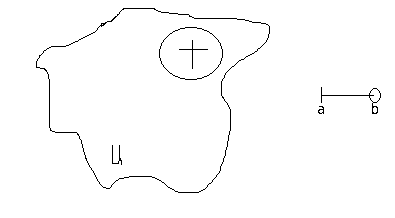
\includegraphics[scale=0.5]{fig3.png}
\caption{}
\end{figure}

Konvergenz und Stetigkeit lassen sich in metrischen Räumen durch offene Mengen beschreiben.
\begin{st}
In einem metrischen Raum konvergiert eine Folge $(x_n)_{n \in \N}$ genau dann gegen x, wenn es zu jeder Umgebung $U$ von $x$ ein $k \in \N$ gibt, so dass $x_n \in U$ für alle $n \ge k $ gilt.\\
\underline{Kurz:} Eine Folge $(x_n)_{n \in \N}$ konvergiert gegen $x$, wenn in jeder Umgebunng von $x$ \emph{fast alle} ($\hat =$ alle bis auf endlich viele) Folgenglieder liegen.
\end{st}
\begin{proof}
Die Äquivalenz gilt, da jede Umgebung von $x$ einen $\eps$-Ball um $x$ enthält und umgekehrt jeden $\eps$-Ball um $x$ auch eine Umgebung von $x$ ist.
\end{proof}
\begin{st}\label{st:1.8}
Eine Abbildung zwischen metrischen Räumen $f: X\rightarrow \tilde X$ ist genau dann stetig in $x \in X$, wenn es zu jeder Umgebung $V$ von $f(X)$ eine Umgebung $U$ von $x$ gibt, so dass U unter $ f $ in V abgebildet wird; oder äquivalent dazu, falls das Urbild jeder Umgebung von $  f(x) $ eine Umgebung von x ist.
\end{st}
\begin{proof}
Dies folgt direkt aus der $ \eps $-$ \delta $-Definition der Stetigkeit und der Definition der Umgebung.
\begin{figure}[h]
\centering
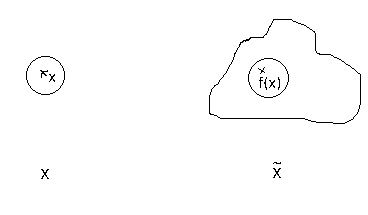
\includegraphics[scale=0.5]{fig4.png}
\caption{}
\end{figure}
\end{proof}
\begin{st}
Eine Abbildung zwischen metrischen Räumen ist stetig genau dann, wenn die Urbilder offener Mengen offen sind.
\end{st}
\begin{proof}
\begin{seg}{"`$\Longrightarrow$"'}
Sei $ f: X \to \tilde X $ stetig und $ V \subset \tilde X $ offen.  Dann ist $ f^{-1}(V) $ nach \ref{st:1.8} eine Umgebung jeder ihrer Punkte somit offen.
\end{seg}

\begin{seg}{"`$\Longleftarrow$"'}
Seien umgekehrt die Urbilder offener Mengen offen und $ x \in X $. Sei $ \eps>0 $.  Nach Voraussetzung $ f^{-1}(B_\eps(f(x)) $ offen und enthält somit einen $ \delta $-Ball um den Punkt x.
\end{seg}
\end{proof}

Wichtige Beobachtung: Um Konvergenz und Stetigkeit zu beschreiben muss man nicht direkt auf eine Metrik Bezug nehmen, sondern es genügt das System der offenen Mengen zu kennen.  Dieses System von offenen Mengen nennt man \emph{die Topologie} des metrischen Raums .  Verschiedene Metriken können dieselbe Topologie erzeugen.

Alle Eigenschaften von metrischen Räumen, ihren Teilmengen oder Abbildung zwischen metrischen Räumen, die sich durch die Topologie (ohne direkten Bezug auf die Metrik) beschreiben lassen, nennen wir \emph{topologische Eigenschaften}.

Dies führt zu dem folgenden Begriff:
\begin{df}
Sei $ X $ eine Menge und $O \subset \mathcal P (x)$ eine Menge von Teilmengen von X; $ O $ heißt eine \emph{Topologie} auf $ X $, wenn folgendes gilt:
\begin{itemize}
\item[(T1)] Beliebige Vereinigungen von Mengen in $ O $ liegen wieder in $O$.
\item[(T2)] Die Schnittmenge von je zwei Mengen in $  O  $ liegt wieder in $O$.
\item[(T3)] Es gilt $ \emptyset \in O $ und $ X \in O$
\end{itemize}
Eine Menge $ X $ zusammen mit einer Topologie auf $ X $ heißt \emph{topologischer Raum}, die Elemente von $ O $ nennt man \emph{offene Teilmengen} von X, ihre Komplemente \emph{abgeschlossene Teilmengen}.
\end{df}
\begin{note*}
\begin{enumerate}[(\roman{enumi})]
\item Natürlich ist die Definition so gemacht, dass die in einem metrischen Raum durch \ref{def:1.1.7} gegebenen offenen Mengen eine Topologie bilden. (Übung) 
\begin{figure}[H]
\centering
\fixme[fig5]
\caption{}
\end{figure}
\item Verschiedene Metriken können diesselbe Topologie erzeugen, vgl. der aus der Analysis bekannter Satz, dass alle Normen auf dem $ \R^n $ äquivalent.
  Daraus folgt: die Metrik $ d(x,y) :=||x-y|| $ definiert für \emph{alle Normen auf $ \R^n $} dieselbe Topologie, die sogenannte \emph{Standardtopologie}, zum Beispiel definieren:
\begin{align*}
d_1(x,y)&=|x_1-y_1|+\dotsb +|x_n-y_n|\\
d_2(x,y)&=\sqrt{(x_1-y_1)^2+\dotsb +(x_n-y_n)^2}\\
d_\infty(x,y)&=\max(|x_1-y_1|, \dotsc  , |x_n-y_n|)
\end{align*}
alle die Standardtopologie.
\end{enumerate}
\end{note*}
\begin{df}
Sei $ X $ ein topologischer Raum und  $x \in X $. Eine Teilmenge $ U \subset X $ heißt \emph{Umgebung} von x, wenn es eine offene Menge $ T\subset U $ gibt, die $ x $ enthält. $ x $ heißt \emph{innerer Punkt} von A, wenn $ A $ eine Umgebung von $ x $ ist. $ x $ heißt \emph{äußerer Punkt}, falls $ X\setminus A $ eine Umgebung von x ist. Der Punkt $ x $ heißt Randpunkt von $ A $, falls keines von beiden gilt.  Die Menge $ \mathring{A} $ der inneren Punkte von $ A $ bezeichnet man als das \emph{Innere} von $ A $ oder als \emph{offener Kern} von $ A $. Die Menge $ \bar A $, der nicht äußeren Punkte von $ A $ heißt \emph{Abschluss} oder \emph{abgeschlossene Hülle} von $ A $.  Die Menge der Randpunkte von $  A $  heißt auch der Rand von A und wird mit $ \delta A $ bezeichnet. 
\end{df}

\begin{ex*}
Sei $ A=[a,b)\subset \R $ und sei $\R$ mit der Standardtopologie versuchen.  Dann gilt $\mathring A=(a,b), \bar A=[a,b], \delta A=\{a,b\}, B=\Q\subset \R$ gilt $ \mathring B=\emptyset, \bar B=\R, \delta B=\R $ 
\end{ex*}
\begin{ex}[Beispiele für Topologien]\label{thm:1.13}
\begin{enumerate}[(\roman{enumi})]
\item Durch Metriken definierte Topologie. Dies sind die sogenannten \emph{metrisierbaren Topologien}.
\item Die \emph{Klumpentopologie} $ O=\{\emptyset, X\} $ für eine beliebige Menge $ X $.  Sie ist nicht metrisierbar (falls $ X $ mehr als ein Element hat)
\item Die \emph{diskrete Topologie} $ O=\mathcal{P}(x) $ ist für jede beliebige Menge $ X $ definiert.  (Nur die schließlich konstanten Folgen sind konvergent.) Sie ist durch die diskrete Metrik gegeben.
\item Auf $\R^2$ ist durch
\[
O=\{A\subset \R^2|\forall_{(x,y)\in A}\exists_{\eps>0}:(x-\eps,x+\eps) \times \{y\} \subset A\}
\]
eine Topologie gegeben. Übung: Ist diese metrisierbar?
\end{enumerate}

\end{ex}

\begin{df}
Sind auf einer Menge $X$ zwei Topologien $ O_1$ und $ O_2 $ gegeben, dann betrachten wir folgende Sprachweisen: gilt $ O_1 \subset O_2 $ , dann sagen wir $ O_2 $ ist \emph{feiner} als $ O_1 $ (und $ O_1 $ ist \emph{gröber} als $ O_2 $).  Gilt weder $ O_1 \subset O_2 $ noch $ O_2\subset O_1 $ , dann sagen wird, die Topologien $ O_1 $ und $ O_2 $ sind \emph{unvergleichbar}.
\end{df}

Auf jeder Menge ist die Klumpentopologie die gröbste mögliche Topologie und die diskrete Topologie, die feinst mögliche Topologie.  Die Topologie in \ref{thm:1.13}(iv) auf $ \R^2 $ ist feiner als die Standardtoplogie, aber gröber als die diskrete.

\begin{df}
Sei $ X $ ein topologischer Raum.  Eine Folge $ (x_n)_{n \in \N} $ heißt konvergent gegen $ a\in X $, falls jede Umgebung von $ a $ fast alle Folgenglieder enthält.
\end{df}
\begin{df}\label{thm:1.16}
Eine Abbildung $ f:X\to Y $ zwischen topologischen Räumen heißt \emph{stetig} in $ x\in X $, falls es zu jeder Umgebung $ V $ von $ f(x) $ eine Umgebung $ U $ von $ x $ gibt,
 so dass $ f(U)\subset V $ (Äquivalent: Falls das Urbild jeder Umgebung von $ f(x) $ eine Umgebung von $ x $ ist). Die Abbildung heißt \emph{stetig}, wenn die Urbilder offener Mengen offen sind. 
Eine Abbildung zwischen topologischen Räumen, die bijektiv und stetig ist, heißt \emph{Homöomorphismus} (falls auch ihre Umkehrabbildung stetig ist).  Falls es einen Homöomorphismus $ d: X\to Y $ gibt, sagt man, $ X $ und $ Y $ sind \emph{homöomorph}, man schreibt: $ X\homo Y $.
Aus der Definition folgt sofort, dass eine Abbildung $ f: X\to Y $ genau dann stetig ist, falls sie in jedem $ x\in X $ stetig ist. (zur Übung nachvollziehen)
\end{df}
\begin{st}\label{thm:1.17}
Sei $ f: X\to Y $ eine (in $ a\in X $) stetige Abbildung zwischen topologischen Räumen.  Sei $ x_n\to a $ konvergente Folge in $ X $. Dann gilt $ f(x_n) \to f(a) $
\end{st}
\begin{proof}
Sei $ V $ eine Umgebung von $ f(a) $. Da $ f $ (in $ a $) stetig ist, ist $ f^{-1}(V) $ eine Umgebung von $a$.  Wegen $ x_n\to a $ liegen fast alle $ x_n $ in $f^{-1}(V)$,
 somit liegen fast alle $f(x_n)$ in $ V $.
\end{proof}
\begin{att}
Eine Abbildung, die jede konvergente Folge auf eine gegen das Bild des Limes konvergierende Folge abbildet (so eine Abbildung heißt \emph{folgenstetig}) ist \emph{im Allgemeinen nicht}
 notwendigerweise stetig. Siehe z. B. Jänich "`Topologie"' 6.3, bzw. später in der Vorlesung.
\end{att}
\begin{ex*}
\begin{enumerate}[(i)]
\item ist $ f: X\to Y $ eine stetige Abbildung und wird die Topologie auf $ X $ durch eine feinere oder die Topologie auf $ Y $ durch eine gröbere ersetzt, bleibt $ f $ stetig.
\item Insbesondere ist \emph{jede} Abbildung $ f: X\to Y $ stetig falls $ Y $ die Klumpentopologie oder $ X $ die diskrete Topologie trägt.
\item In der Klumpentopologie ist \emph{jede} Folge gegen \emph{jeden Punkt} konvergent. 
\end{enumerate}
\end{ex*}
\begin{note}
Die Axiome eines topologischen Raums sind für sich alleine relativ schwach und lassen sehr viele Beispiele auch mit "`pathologischen"' Eigenschaften zu. Sie sind eher ein äußerer Begriffsrahmen. Um etwa Räume mit den von metrischen Räumen vertrauten Eigenschaften zu erhalten, muss man Zusatzannahmen machen.
\begin{itemize}
  \item "`Hausdorffeigenschaft"' $\implies$ Eindeutigkeit des Limes
  \item "`Abzählbarkeitsaxiome"' $\implies$ Äquivalenz von Stetigkeit und Folgenstetigkeit
\end{itemize}
\end{note}
\subsection{Grundkonstruktionen}
Grundkonstruktionen sind Methoden, um neue Topologien zu definieren durch:
\begin{itemize}
\item Summe, Teilräume, Produkte, Quotienten
\item durch Abbildungen zwischen topologischen Räumen
\end{itemize}
\begin{df}
Seien $ X $ und $ Y $ topologische Räume. Auf der disjunkten Vereinigung $ X \mathbin{\dot{\cup}} V =X \times \{ 0 \} \cup Y \times \{1\}$ definieren wir eine Topologie durch:
\[
\{U \mathbin{\dot{\cup}} V| U \text{ offen in } X, V \text{ offen in } Y\}
\]
Der so entstehende topologische Raum $ X+Y $ wird als topologische Summe von X und Y bezeichnet (andere übliche Zeichen: $X \sqcup Y$ oder auch $X \perp Y$).
\end{df}
\begin{note*}
\begin{enumerate}[(i)]
\item Analog definiert man die Summen von beliebig (auch unendlich) vielen topologischer Räumen $\biguplus_{\alpha \in  A} X_\alpha=\bigsqcup_{\alpha\in A} X_\alpha$, indem man wiederum als offene Mengen $\{\dot \bigcup_{\alpha\in A} U_\alpha | U_\alpha \text{ offen in } X_\alpha \}$ setzt.
\item Für die disjunkte Verreinigung von Mengen $ X \dotcup Y $ ist auch die Schreibweise $X+Y:= X\times\{0\} \cup Y\times \{1\}$ üblich.  
\end{enumerate}
\end{note*}
\begin{ex*}
\begin{enumerate}[(i)]
\item Sei $ X=\{ x\} $ eine einelementige Menge mit Klumpen- bzw. diskreter Topologie. Dann ist die topologische Summe $ \biguplus_{\alpha\in A}X $ homöomorph zu $A$, mit der diskreten Topologie versehen (für eine beliebige Menge $A$). 
\item Beispiel \ref{thm:1.13}(iv) ist homöomorph zu $ \biguplus_{\alpha\in \R}  \R $ (Übung)
\end{enumerate}
\end{ex*}
\begin{df} Sei $ X $ ein topologischer Raum und $ M \subset X $. Die durch $ \{ U\cap M| U \text{ offen in } X \}$ auf $M$ definierte Topologie heißt \emph{Teilraumtopologie} (auch \emph{induzierte}, \emph{Relativ-} oder \emph{Spurtopologie}). 
\end{df}
\begin{ex*}
$X=\R^2, M=\{x-\text{Achse}\}$
\begin{figure}[ht]
\centering



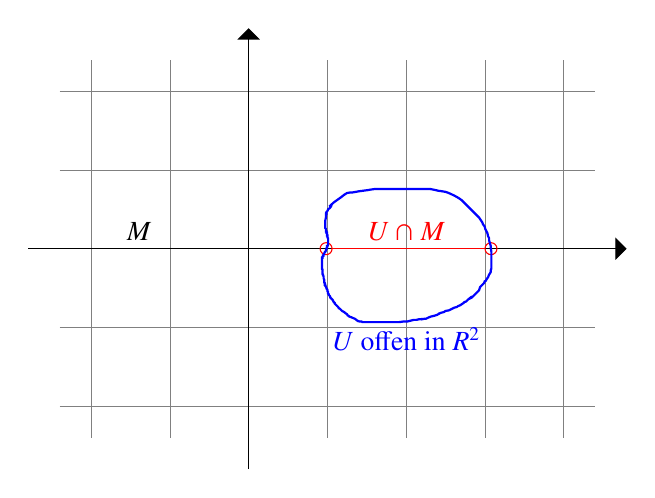
\begin{tikzpicture}[y=0.80pt, x=0.8pt, inner sep=0pt, outer sep=0pt]
\begin{scope}[scale=2,xshift=40,yshift=140,y=1cm,x=1cm]
\draw[step=.5cm,gray,very thin] (-1.2,-1.2) grid (2.2,1.2);
\draw [-triangle 90] (-1.4,0) -- (2.4,0);
\draw [-triangle 90] (0,-1.4) -- (0,1.4); 
\draw (-0.7,0.05) node [anchor=south] {$M$};
\draw [blue] (1,-0.5) node [anchor=north] {$U$ offen in $R^2$};
\draw [red] (1,0.05) node [anchor=south] {$U\cap M$};
\draw [red,o-o] (0.45,0) -- (1.58,0);
\end{scope}


\begin{scope}[scale=0.5]
\path[draw=blue,line join=miter,line cap=butt,line width=0.800pt]
  (269.7107,728.1032) .. controls (269.7107,728.9450) and (269.7107,729.7868) ..
  (269.7107,730.6286) .. controls (269.7107,731.8665) and (269.4848,732.1794) ..
  (270.2158,733.1540) .. controls (270.5015,733.5349) and (270.9810,733.7558) ..
  (271.2260,734.1641) .. controls (271.4999,734.6207) and (271.3985,735.2636) ..
  (271.7310,735.6794) .. controls (272.1102,736.1534) and (272.8577,736.2232) ..
  (273.2463,736.6895) .. controls (277.6350,741.9560) and (268.9009,734.5161) ..
  (276.7818,741.7403) .. controls (277.8494,742.7189) and (279.1388,743.4239) ..
  (280.3173,744.2657) .. controls (281.4958,745.1074) and (282.6697,745.9558) ..
  (283.8529,746.7910) .. controls (285.5318,747.9762) and (286.9955,749.5633) ..
  (288.9036,750.3266) .. controls (290.4746,750.9550) and (292.2794,750.5924) ..
  (293.9544,750.8316) .. controls (295.8178,751.0978) and (297.6498,751.5556) ..
  (299.5102,751.8418) .. controls (302.0283,752.2292) and (304.5643,752.4916) ..
  (307.0864,752.8519) .. controls (309.2785,753.1651) and (311.4445,753.6923) ..
  (313.6524,753.8621) .. controls (315.8346,754.0300) and (318.0297,753.8621) ..
  (320.2184,753.8621) .. controls (329.1414,753.8621) and (338.0644,753.8621) ..
  (346.9874,753.8621) .. controls (349.8495,753.8621) and (352.7116,753.8621) ..
  (355.5737,753.8621) .. controls (358.4358,753.8621) and (361.3112,754.1378) ..
  (364.1600,753.8621) .. controls (366.5593,753.6299) and (368.8608,752.7858) ..
  (371.2311,752.3469) .. controls (373.4085,751.9437) and (375.6544,751.8957) ..
  (377.7971,751.3367) .. controls (379.5516,750.8790) and (381.1943,750.0605) ..
  (382.8478,749.3164) .. controls (386.0646,747.8689) and (389.6826,746.0045) ..
  (392.4443,743.7606) .. controls (393.7378,742.7096) and (394.8013,741.4036) ..
  (395.9798,740.2250) .. controls (396.8216,739.3832) and (397.6634,738.5415) ..
  (398.5052,737.6997) .. controls (400.8622,735.3426) and (403.2192,732.9856) ..
  (405.5763,730.6286) .. controls (406.0813,730.1235) and (406.5864,729.6184) ..
  (407.0915,729.1134) .. controls (407.4282,728.7766) and (407.8042,728.4751) ..
  (408.1016,728.1032) .. controls (408.8600,727.1552) and (409.4485,726.0829) ..
  (410.1219,725.0728) .. controls (410.4587,724.5677) and (410.8606,724.1005) ..
  (411.1321,723.5575) .. controls (411.3702,723.0813) and (411.3730,722.5045) ..
  (411.6372,722.0423) .. controls (412.0548,721.3114) and (412.7759,720.7749) ..
  (413.1524,720.0220) .. controls (413.4628,719.4011) and (413.4137,718.6517) ..
  (413.6575,718.0017) .. controls (414.1862,716.5917) and (415.2016,715.3897) ..
  (415.6778,713.9611) .. controls (415.9492,713.1467) and (415.9114,712.2501) ..
  (416.1829,711.4357) .. controls (416.4209,710.7214) and (417.0104,710.1458) ..
  (417.1930,709.4154) .. controls (417.3563,708.7621) and (417.0609,708.0554) ..
  (417.1930,707.3951) .. controls (417.6813,704.9538) and (418.4282,704.5842) ..
  (418.7082,702.3443) .. controls (418.7917,701.6761) and (418.6412,700.9941) ..
  (418.7082,700.3240) .. controls (418.8101,699.3050) and (419.1283,698.3141) ..
  (419.2133,697.2936) .. controls (419.2972,696.2869) and (419.2133,695.2733) ..
  (419.2133,694.2631) .. controls (419.2133,693.2530) and (419.2133,692.2428) ..
  (419.2133,691.2327) .. controls (419.2133,689.5491) and (419.2133,687.8655) ..
  (419.2133,686.1819) .. controls (419.2133,685.5085) and (419.2133,684.8350) ..
  (419.2133,684.1616) .. controls (419.2133,683.4881) and (419.3085,682.8079) ..
  (419.2133,682.1413) .. controls (419.1380,681.6142) and (418.7958,681.1512) ..
  (418.7082,680.6261) .. controls (418.6252,680.1278) and (418.8072,679.6061) ..
  (418.7082,679.1108) .. controls (418.5928,678.5336) and (417.3460,676.8404) ..
  (417.1930,676.5854) .. controls (415.8690,674.3788) and (417.6283,676.9510) ..
  (416.1829,674.0601) .. controls (416.0764,673.8471) and (415.8206,673.7455) ..
  (415.6778,673.5550) .. controls (415.3136,673.0694) and (414.9799,672.5603) ..
  (414.6676,672.0398) .. controls (414.4739,671.7169) and (414.4287,671.2958) ..
  (414.1625,671.0296) .. controls (413.8964,670.7634) and (413.3783,670.8257) ..
  (413.1524,670.5245) .. controls (412.8330,670.0986) and (412.9212,669.4658) ..
  (412.6473,669.0093) .. controls (412.4023,668.6010) and (411.9739,668.3359) ..
  (411.6372,667.9991) .. controls (411.3004,667.6624) and (410.9637,667.3257) ..
  (410.6270,666.9890) .. controls (410.1219,666.4839) and (409.4662,666.0939) ..
  (409.1118,665.4738) .. controls (408.0873,663.6809) and (409.1493,663.7529) ..
  (408.1016,662.4433) .. controls (407.6554,661.8855) and (407.0915,661.4332) ..
  (406.5864,660.9281) .. controls (405.5763,659.9179) and (404.5661,658.9078) ..
  (403.5559,657.8976) .. controls (403.2192,657.5609) and (402.8825,657.2242) ..
  (402.5458,656.8875) .. controls (402.2091,656.5507) and (401.9440,656.1223) ..
  (401.5356,655.8773) .. controls (397.8014,653.6368) and (402.3369,657.4274) ..
  (398.5052,654.3621) .. controls (397.7615,653.7671) and (397.3015,652.8318) ..
  (396.4849,652.3418) .. controls (396.0284,652.0679) and (395.4262,652.1106) ..
  (394.9697,651.8367) .. controls (394.5613,651.5917) and (394.3313,651.1240) ..
  (393.9595,650.8266) .. controls (393.4855,650.4473) and (392.9493,650.1531) ..
  (392.4443,649.8164) .. controls (391.9392,649.4797) and (391.4720,649.0777) ..
  (390.9290,648.8062) .. controls (390.4528,648.5682) and (389.8900,648.5393) ..
  (389.4138,648.3012) .. controls (388.8709,648.0297) and (388.4565,647.5301) ..
  (387.8986,647.2910) .. controls (387.2605,647.0176) and (386.5282,647.0297) ..
  (385.8783,646.7859) .. controls (383.6335,645.9441) and (383.3529,645.1024) ..
  (380.8275,644.2606) .. controls (379.8560,643.9367) and (378.7686,644.0793) ..
  (377.7971,643.7555) .. controls (377.2212,643.5635) and (376.8398,642.9844) ..
  (376.2818,642.7453) .. controls (375.6438,642.4719) and (374.9201,642.4598) ..
  (374.2615,642.2403) .. controls (369.0183,640.4925) and (373.9328,642.0759) ..
  (370.2209,640.2199) .. controls (368.6224,639.4207) and (366.3698,639.2730) ..
  (364.6651,638.7047) .. controls (363.8050,638.4180) and (362.9682,638.0628) ..
  (362.1397,637.6946) .. controls (361.4517,637.3888) and (360.8433,636.8913) ..
  (360.1194,636.6844) .. controls (359.6337,636.5457) and (359.1053,636.7471) ..
  (358.6042,636.6844) .. controls (350.9398,635.1515) and (361.1670,637.0253) ..
  (353.5534,636.1793) .. controls (352.8635,636.1026) and (352.2230,635.7509) ..
  (351.5331,635.6743) .. controls (350.6964,635.5813) and (349.8380,635.8127) ..
  (349.0077,635.6743) .. controls (345.8670,635.1508) and (345.8194,634.3984) ..
  (342.9468,634.1590) .. controls (341.7724,634.0611) and (340.5868,634.2430) ..
  (339.4113,634.1590) .. controls (338.2238,634.0742) and (337.0613,633.7617) ..
  (335.8757,633.6540) .. controls (335.2051,633.5930) and (334.5289,633.6540) ..
  (333.8554,633.6540) .. controls (332.8453,633.6540) and (331.8351,633.6540) ..
  (330.8250,633.6540) .. controls (328.8047,633.6540) and (326.7844,633.6540) ..
  (324.7640,633.6540) .. controls (319.7133,633.6540) and (314.6625,633.6540) ..
  (309.6118,633.6540) .. controls (307.9282,633.6540) and (306.2446,633.6540) ..
  (304.5610,633.6540) .. controls (304.4410,633.6540) and (302.6539,633.5974) ..
  (302.5407,633.6540) .. controls (302.3277,633.7604) and (302.2486,634.0526) ..
  (302.0356,634.1590) .. controls (301.7009,634.3264) and (300.4386,634.0179) ..
  (300.0153,634.1590) .. controls (299.6582,634.2781) and (299.3623,634.5451) ..
  (299.0052,634.6641) .. controls (298.8454,634.7173) and (298.6598,634.6109) ..
  (298.5001,634.6641) .. controls (296.8406,635.2173) and (297.2421,635.9602) ..
  (295.9747,636.6844) .. controls (295.1875,637.1342) and (294.2827,637.3374) ..
  (293.4493,637.6946) .. controls (293.1033,637.8429) and (292.7887,638.0598) ..
  (292.4392,638.1996) .. controls (291.9448,638.3974) and (291.4001,638.4666) ..
  (290.9239,638.7047) .. controls (290.7110,638.8112) and (290.6170,639.0777) ..
  (290.4189,639.2098) .. controls (290.1056,639.4186) and (289.6749,639.4487) ..
  (289.4087,639.7149) .. controls (289.1425,639.9811) and (289.1698,640.4588) ..
  (288.9036,640.7250) .. controls (288.4744,641.1543) and (287.8740,641.3710) ..
  (287.3884,641.7352) .. controls (287.1979,641.8780) and (287.0738,642.0974) ..
  (286.8833,642.2403) .. controls (286.3977,642.6045) and (285.8886,642.9381) ..
  (285.3681,643.2504) .. controls (285.0453,643.4441) and (284.6591,643.5296) ..
  (284.3579,643.7555) .. controls (283.5960,644.3269) and (283.0995,645.2044) ..
  (282.3376,645.7758) .. controls (282.0365,646.0017) and (281.5937,646.0147) ..
  (281.3275,646.2809) .. controls (281.0613,646.5471) and (281.0312,646.9778) ..
  (280.8224,647.2910) .. controls (280.6903,647.4891) and (280.4857,647.6277) ..
  (280.3173,647.7961) .. controls (279.6439,648.4695) and (278.9705,649.1430) ..
  (278.2970,649.8164) .. controls (278.1287,649.9848) and (277.8984,650.1085) ..
  (277.7920,650.3215) .. controls (277.7167,650.4721) and (277.8854,650.6865) ..
  (277.7920,650.8266) .. controls (277.5278,651.2228) and (277.0675,651.4558) ..
  (276.7818,651.8367) .. controls (276.3300,652.4390) and (276.1893,653.2305) ..
  (275.7717,653.8570) .. controls (275.2762,654.6002) and (274.2468,655.1341) ..
  (273.7513,655.8773) .. controls (273.6579,656.0174) and (273.7513,656.2140) ..
  (273.7513,656.3824) .. controls (273.5830,656.7191) and (273.4721,657.0914) ..
  (273.2463,657.3925) .. controls (272.9606,657.7735) and (272.5003,658.0065) ..
  (272.2361,658.4027) .. controls (272.1427,658.5428) and (272.3114,658.7572) ..
  (272.2361,658.9078) .. controls (272.1296,659.1207) and (271.7888,659.1819) ..
  (271.7310,659.4128) .. controls (271.6085,659.9028) and (271.8535,660.4381) ..
  (271.7310,660.9281) .. controls (271.6733,661.1591) and (271.3013,661.2073) ..
  (271.2260,661.4332) .. controls (271.1195,661.7526) and (271.3077,662.1166) ..
  (271.2260,662.4433) .. controls (270.6162,664.8823) and (270.9859,662.4183) ..
  (270.2158,663.9585) .. controls (270.1405,664.1091) and (270.2690,664.3039) ..
  (270.2158,664.4636) .. controls (270.0968,664.8208) and (269.8298,665.1166) ..
  (269.7107,665.4738) .. controls (269.6575,665.6335) and (269.7860,665.8283) ..
  (269.7107,665.9788) .. controls (269.6043,666.1918) and (269.2810,666.2580) ..
  (269.2056,666.4839) .. controls (269.0992,666.8034) and (269.3562,667.1929) ..
  (269.2056,667.4941) .. controls (269.1303,667.6447) and (268.8196,667.3750) ..
  (268.7006,667.4941) .. controls (268.7001,667.4945) and (268.7013,669.0070) ..
  (268.7006,669.0093) .. controls (268.6253,669.2352) and (268.3020,669.3014) ..
  (268.1955,669.5144) .. controls (268.0451,669.8151) and (268.3372,671.6145) ..
  (268.1955,672.0398) .. controls (268.0764,672.3969) and (267.8095,672.6928) ..
  (267.6904,673.0499) .. controls (267.5115,673.5866) and (267.8693,674.5335) ..
  (267.6904,675.0702) .. controls (267.6151,675.2961) and (267.2606,675.3494) ..
  (267.1853,675.5753) .. controls (267.0789,675.8947) and (267.2918,676.2660) ..
  (267.1853,676.5854) .. controls (267.1100,676.8113) and (266.7556,676.8646) ..
  (266.6803,677.0905) .. controls (266.5941,677.3491) and (266.6803,679.7599) ..
  (266.6803,680.1210) .. controls (266.6803,680.2893) and (266.6803,680.4577) ..
  (266.6803,680.6261) .. controls (266.6803,680.7944) and (266.7556,680.9805) ..
  (266.6803,681.1311) .. controls (266.5738,681.3441) and (266.2505,681.4103) ..
  (266.1752,681.6362) .. controls (266.0155,682.1154) and (266.1752,682.6464) ..
  (266.1752,683.1514) .. controls (266.1752,684.3299) and (266.1752,685.5085) ..
  (266.1752,686.6870) .. controls (266.1752,688.2022) and (266.1752,689.7174) ..
  (266.1752,691.2327) .. controls (266.1752,691.4010) and (266.0561,691.6187) ..
  (266.1752,691.7377) .. controls (266.2942,691.8568) and (266.5612,691.6187) ..
  (266.6803,691.7377) .. controls (266.9184,691.9758) and (266.5297,692.4467) ..
  (266.6803,692.7479) .. controls (266.7867,692.9608) and (267.0789,693.0400) ..
  (267.1853,693.2530) .. controls (267.2606,693.4035) and (267.0663,693.6390) ..
  (267.1853,693.7580) .. controls (267.3044,693.8771) and (267.5714,693.6390) ..
  (267.6904,693.7580) .. controls (267.9285,693.9961) and (267.5398,694.4670) ..
  (267.6904,694.7682) .. controls (267.7969,694.9811) and (268.0890,695.0603) ..
  (268.1955,695.2733) .. controls (268.2708,695.4238) and (268.1955,695.6100) ..
  (268.1955,695.7783) .. controls (268.3639,696.1151) and (268.4917,696.4753) ..
  (268.7006,696.7885) .. controls (269.4711,697.9443) and (269.1004,696.4727) ..
  (269.7107,698.3037) .. controls (269.7639,698.4634) and (269.6354,698.6582) ..
  (269.7107,698.8088) .. controls (269.8172,699.0218) and (270.1093,699.1009) ..
  (270.2158,699.3139) .. controls (270.3664,699.6150) and (270.0652,700.0229) ..
  (270.2158,700.3240) .. controls (270.3223,700.5370) and (270.6144,700.6161) ..
  (270.7209,700.8291) .. controls (270.8210,701.0294) and (270.6176,702.2411) ..
  (270.7209,702.3443) .. controls (270.8399,702.4634) and (271.1069,702.2253) ..
  (271.2260,702.3443) .. controls (271.3450,702.4634) and (271.1507,702.6988) ..
  (271.2260,702.8494) .. controls (271.3324,703.0624) and (271.6246,703.1415) ..
  (271.7310,703.3545) .. controls (271.7963,703.4851) and (271.7310,706.0269) ..
  (271.7310,706.3849) .. controls (271.7310,706.7429) and (271.7963,709.2848) ..
  (271.7310,709.4154) .. controls (271.6246,709.6284) and (271.3324,709.7075) ..
  (271.2260,709.9205) .. controls (271.0890,710.1945) and (271.3642,711.8026) ..
  (271.2260,711.9408) .. controls (271.1069,712.0598) and (270.8399,711.8217) ..
  (270.7209,711.9408) .. controls (270.5660,712.0956) and (270.8770,714.3101) ..
  (270.7209,714.4662) .. controls (270.6018,714.5852) and (270.3349,714.3471) ..
  (270.2158,714.4662) .. controls (269.9777,714.7043) and (270.4539,715.2382) ..
  (270.2158,715.4763) .. controls (270.0968,715.5954) and (269.8298,715.3573) ..
  (269.7107,715.4763) .. controls (269.5334,715.6536) and (269.8852,717.6528) ..
  (269.7107,718.0017) .. controls (269.6043,718.2147) and (269.3121,718.2938) ..
  (269.2056,718.5068) .. controls (269.1404,718.6374) and (269.2056,721.1792) ..
  (269.2056,721.5372) .. controls (269.2056,722.5474) and (269.2056,723.5575) ..
  (269.2056,724.5677) .. controls (269.2056,724.9044) and (269.1504,725.2457) ..
  (269.2056,725.5778) .. controls (269.3468,726.4246) and (269.6253,727.2490) ..
  (269.7107,728.1032) .. controls (269.7945,728.9408) and (269.7107,729.7868) ..
  (269.7107,730.6286) .. controls (269.7107,730.7970) and (269.7107,730.9653) ..
  (269.7107,731.1337) .. controls (269.7107,731.3020) and (269.5917,731.5197) ..
  (269.7107,731.6388) .. controls (269.8298,731.7578) and (270.0968,731.5197) ..
  (270.2158,731.6388) .. controls (270.3349,731.7578) and (270.2158,731.9755) ..
  (270.2158,732.1438) .. controls (270.2158,732.3122) and (270.2158,732.4805) ..
  (270.2158,732.6489) -- cycle;
\end{scope}
\end{tikzpicture}

\caption{}
\end{figure}
\end{ex*}
\begin{att*}
Die offene Mengen $U\cap M$ in $ M $ sind im Allgemeinen nicht offen in $ X $ (es sei denn $ M\subset X $ wäre offen). Zum Beispiel:
\[
\text{T2: } (\underbrace{U_1}_{\text{offen in }X}\cap M)\cap (\underbrace{U_2}_{\text{offen in }X}\cap M)=(U_1\cap U_2)\cap M
\]
\end{att*}
\begin{df}
Seien $ X $ und $ Y $ topologische Räume. Eine Teilmenge $ W\subset X\times Y $ heißt offen bezüglich der Produkttopologie auf $ X\times Y $ , falls es zu jedem Punkt $ (x,y)\in W $ eine Umgebung $ U $ von $ x $ und eine Umgebung $ V $ von $ y $ gibt, sodass $ U\times V $ in W enthalten ist.
\begin{figure}[ht]
\centering



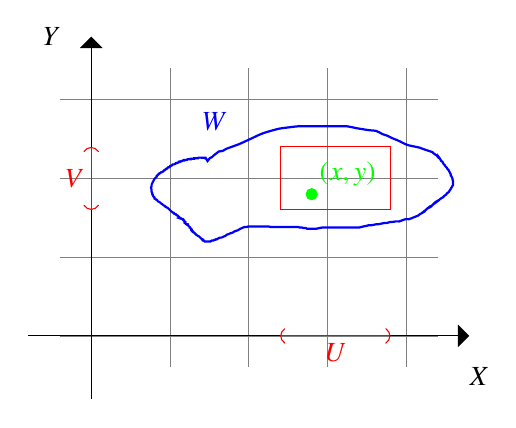
\begin{tikzpicture}[scale=1,y=0.80pt, x=0.8pt, inner sep=0pt, outer sep=0pt]
\begin{scope}[scale=2,xshift=40,yshift=112,y=1cm,x=1cm]
\draw[step=.5cm,gray,very thin] (-0.2,-0.2) grid (2.2,1.7);
\draw [-triangle 90] (-0.4,0) -- (2.4,0);
\draw [-triangle 90] (0,-0.4) -- (0,1.9); 
\draw (-0.2,1.9) node [anchor=east] {$Y$};
\draw (2.4,-0.2) node [anchor=north west] {$X$};


\begin{scope}[red]
\draw [(-)] (1.2,0) -- (1.9,0);
\draw (1.55,- 0.05) node [anchor=north] {$U$};
\draw [(-)] (0,0.8) -- (0,1.2);
\draw  (-0.05,1) node [anchor=east] {$V$};
\draw (1.2,0.8) rectangle (1.9,1.2);
\end{scope}
\filldraw [green] (1.4,0.9) circle (1pt);
\draw  [green](1.45,0.95) node [anchor=south west] {$(x,y)$};
\draw  [blue](0.7,1.3) node [anchor=south west] {$W$};
\end{scope}
\begin{scope} [scale=0.5]
\path[draw=blue,line join=miter,line cap=butt,line width=0.800pt]
  (305.0661,718.0017) .. controls (305.7395,718.8435) and (306.2751,719.8172) ..
  (307.0864,720.5271) .. controls (307.6530,721.0229) and (308.4940,721.0996) ..
  (309.1067,721.5372) .. controls (309.6879,721.9524) and (310.0796,722.5876) ..
  (310.6219,723.0525) .. controls (311.2611,723.6003) and (311.9777,724.0509) ..
  (312.6422,724.5677) .. controls (313.4932,725.2295) and (314.1725,726.1734) ..
  (315.1676,726.5880) .. controls (316.2665,727.0459) and (317.5820,726.6927) ..
  (318.7031,727.0931) .. controls (319.9814,727.5496) and (321.0105,728.5354) ..
  (322.2387,729.1134) .. controls (327.8539,731.7558) and (327.2285,730.7585) ..
  (333.3503,733.1540) .. controls (335.2448,733.8953) and (337.0569,734.8318) ..
  (338.9062,735.6794) .. controls (341.0975,736.6837) and (343.2858,737.6947) ..
  (345.4722,738.7098) .. controls (347.9998,739.8834) and (350.4608,741.2104) ..
  (353.0483,742.2454) .. controls (357.1928,743.9032) and (366.2134,746.4710) ..
  (370.2209,747.2961) .. controls (372.7163,747.8099) and (375.2690,747.9903) ..
  (377.7971,748.3063) .. controls (380.6566,748.6637) and (383.5065,749.1472) ..
  (386.3834,749.3164) .. controls (389.2405,749.4845) and (392.1076,749.3164) ..
  (394.9697,749.3164) .. controls (397.6634,749.3164) and (400.3571,749.3164) ..
  (403.0509,749.3164) .. controls (410.2903,749.3164) and (417.5297,749.3164) ..
  (424.7691,749.3164) .. controls (426.9578,749.3164) and (429.1589,749.5496) ..
  (431.3351,749.3164) .. controls (433.8959,749.0421) and (436.3789,748.2701) ..
  (438.9113,747.8012) .. controls (440.9252,747.4282) and (442.9497,747.1146) ..
  (444.9722,746.7910) .. controls (447.1588,746.4412) and (449.3409,746.0556) ..
  (451.5382,745.7809) .. controls (453.3834,745.5502) and (455.2663,745.6185) ..
  (457.0940,745.2758) .. controls (459.2087,744.8793) and (461.3339,743.0420) ..
  (463.1549,742.2454) .. controls (464.6182,741.6052) and (466.2237,741.3383) ..
  (467.7006,740.7301) .. controls (469.0930,740.1568) and (470.3652,739.3214) ..
  (471.7412,738.7098) .. controls (473.3982,737.9734) and (475.1384,737.4336) ..
  (476.7920,736.6895) .. controls (480.9840,734.8031) and (482.4847,733.4665) ..
  (486.8935,732.1438) .. controls (490.0246,731.2045) and (493.3539,731.0459) ..
  (496.4900,730.1235) .. controls (497.8700,729.7176) and (499.1576,729.0374) ..
  (500.5306,728.6083) .. controls (504.4521,727.3828) and (504.5540,728.0567) ..
  (508.1067,726.0829) .. controls (508.5230,725.8517) and (508.7450,725.3702) ..
  (509.1169,725.0728) .. controls (510.5508,723.9256) and (511.2305,723.9693) ..
  (512.6524,722.5474) .. controls (512.9186,722.2812) and (512.8913,721.8034) ..
  (513.1575,721.5372) .. controls (515.7386,718.9561) and (512.4531,723.6550) ..
  (515.1778,720.0220) .. controls (515.6295,719.4197) and (515.6556,718.5341) ..
  (516.1880,718.0017) .. controls (516.4542,717.7355) and (516.9319,717.7628) ..
  (517.1981,717.4966) .. controls (517.7305,716.9642) and (517.7565,716.0787) ..
  (518.2083,715.4763) .. controls (520.3929,713.2917) and (518.2875,715.6101) ..
  (519.7235,713.4560) .. controls (520.1197,712.8617) and (520.8101,712.5122) ..
  (521.2387,711.9408) .. controls (521.4646,711.6396) and (521.5179,711.2318) ..
  (521.7438,710.9306) .. controls (522.0295,710.5497) and (522.4682,710.3014) ..
  (522.7539,709.9205) .. controls (522.9798,709.6193) and (523.0907,709.2470) ..
  (523.2590,708.9103) .. controls (523.4274,708.5736) and (523.5957,708.2369) ..
  (523.7641,707.9002) .. controls (523.9325,707.5635) and (524.1008,707.2267) ..
  (524.2692,706.8900) .. controls (524.4375,706.5533) and (524.6829,706.2451) ..
  (524.7743,705.8799) .. controls (524.8560,705.5532) and (524.6678,705.1892) ..
  (524.7743,704.8697) .. controls (524.8496,704.6438) and (525.1473,704.5627) ..
  (525.2793,704.3646) .. controls (525.4882,704.0514) and (525.6160,703.6912) ..
  (525.7844,703.3545) .. controls (525.9528,703.0178) and (526.1982,702.7096) ..
  (526.2895,702.3443) .. controls (526.3712,702.0177) and (526.2078,701.6608) ..
  (526.2895,701.3342) .. controls (526.3808,700.9690) and (526.7033,700.6892) ..
  (526.7946,700.3240) .. controls (526.9171,699.8340) and (526.7946,699.3139) ..
  (526.7946,698.8088) .. controls (526.7946,698.3037) and (526.7946,697.7986) ..
  (526.7946,697.2936) .. controls (526.7946,696.9569) and (526.8763,696.6101) ..
  (526.7946,696.2834) .. controls (526.6296,695.6237) and (525.5121,694.1460) ..
  (525.2793,693.7580) .. controls (522.9497,689.8753) and (527.4874,696.8175) ..
  (523.7641,691.2327) .. controls (523.4274,690.7276) and (523.1832,690.1467) ..
  (522.7539,689.7174) .. controls (522.3247,689.2882) and (521.6680,689.1365) ..
  (521.2387,688.7073) .. controls (520.9725,688.4411) and (520.9998,687.9633) ..
  (520.7336,687.6971) .. controls (520.3044,687.2679) and (519.6847,687.0756) ..
  (519.2184,686.6870) .. controls (518.6697,686.2297) and (518.2609,685.6179) ..
  (517.7032,685.1717) .. controls (517.4092,684.9366) and (517.0158,684.8603) ..
  (516.6930,684.6667) .. controls (516.1725,684.3543) and (515.6518,684.0357) ..
  (515.1778,683.6565) .. controls (514.8060,683.3590) and (514.5395,682.9438) ..
  (514.1677,682.6464) .. controls (510.1911,679.4651) and (515.4712,684.0826) ..
  (510.6321,680.6261) .. controls (510.0509,680.2109) and (509.6220,679.6159) ..
  (509.1169,679.1108) .. controls (508.6118,678.6057) and (508.1067,678.1007) ..
  (507.6017,677.5956) .. controls (507.2649,677.2589) and (506.9998,676.8304) ..
  (506.5915,676.5854) .. controls (502.8572,674.3449) and (507.3928,678.1356) ..
  (503.5610,675.0702) .. controls (502.8174,674.4753) and (502.3026,673.6213) ..
  (501.5407,673.0499) .. controls (501.2396,672.8240) and (500.8318,672.7707) ..
  (500.5306,672.5448) .. controls (497.3587,670.1659) and (502.1252,672.9965) ..
  (498.0052,670.5245) .. controls (497.6824,670.3308) and (497.2962,670.2453) ..
  (496.9951,670.0194) .. controls (495.3260,668.7677) and (496.7213,669.2028) ..
  (494.9748,668.5042) .. controls (494.4804,668.3065) and (493.9538,668.1969) ..
  (493.4595,667.9991) .. controls (493.1100,667.8593) and (492.7989,667.6339) ..
  (492.4494,667.4941) .. controls (491.9551,667.2963) and (491.4285,667.1867) ..
  (490.9341,666.9890) .. controls (490.5846,666.8492) and (490.2735,666.6237) ..
  (489.9240,666.4839) .. controls (489.4297,666.2862) and (488.9138,666.1472) ..
  (488.4088,665.9788) .. controls (487.9037,665.8105) and (487.4206,665.5491) ..
  (486.8935,665.4738) .. controls (483.6051,665.0040) and (486.0559,666.2047) ..
  (482.3478,664.9687) .. controls (479.8488,664.1357) and (480.9269,663.6916) ..
  (478.3072,663.4535) .. controls (471.3350,663.4535) and (478.0306,663.6472) ..
  (471.7412,662.9484) .. controls (471.2393,662.8926) and (470.7213,663.0474) ..
  (470.2260,662.9484) .. controls (469.0241,662.7080) and (467.8995,662.1397) ..
  (466.6905,661.9382) .. controls (465.8601,661.7998) and (465.0017,662.0312) ..
  (464.1651,661.9382) .. controls (463.4752,661.8616) and (462.8224,661.5837) ..
  (462.1448,661.4332) .. controls (461.3068,661.2469) and (460.4726,661.0229) ..
  (459.6194,660.9281) .. controls (458.9501,660.8537) and (458.2673,661.0116) ..
  (457.5991,660.9281) .. controls (456.9103,660.8420) and (456.2522,660.5914) ..
  (455.5788,660.4230) .. controls (454.5687,660.2546) and (453.5673,660.0198) ..
  (452.5483,659.9179) .. controls (451.8783,659.8509) and (451.1963,660.0014) ..
  (450.5280,659.9179) .. controls (449.8392,659.8318) and (449.1854,659.5634) ..
  (448.5077,659.4128) .. controls (447.6697,659.2266) and (446.8188,659.1008) ..
  (445.9824,658.9078) .. controls (444.6296,658.5956) and (443.3112,658.1259) ..
  (441.9417,657.8976) .. controls (441.2775,657.7869) and (440.5949,657.8976) ..
  (439.9214,657.8976) .. controls (437.3961,657.8976) and (434.8707,657.8976) ..
  (432.3453,657.8976) .. controls (427.7996,657.8976) and (423.2539,657.8976) ..
  (418.7082,657.8976) .. controls (417.1930,657.8976) and (415.6778,657.8976) ..
  (414.1625,657.8976) .. controls (412.3106,657.8976) and (410.4503,658.0732) ..
  (408.6067,657.8976) .. controls (406.8975,657.7348) and (405.2596,657.1004) ..
  (403.5559,656.8875) .. controls (402.5536,656.7622) and (401.5356,656.8875) ..
  (400.5255,656.8875) .. controls (399.3470,656.8875) and (398.1685,656.8875) ..
  (396.9900,656.8875) .. controls (396.3165,656.8875) and (395.6339,656.7767) ..
  (394.9697,656.8875) .. controls (394.5983,656.9494) and (394.3247,657.3012) ..
  (393.9595,657.3925) .. controls (393.3062,657.5559) and (392.5996,657.2605) ..
  (391.9392,657.3925) .. controls (391.4171,657.4970) and (390.9290,657.7293) ..
  (390.4240,657.8976) .. controls (389.7505,657.8976) and (389.0703,657.8024) ..
  (388.4037,657.8976) .. controls (387.8766,657.9729) and (387.4155,658.3274) ..
  (386.8884,658.4027) .. controls (386.2218,658.4979) and (385.5416,658.4027) ..
  (384.8681,658.4027) .. controls (384.0263,658.4027) and (383.1845,658.4027) ..
  (382.3427,658.4027) .. controls (377.9654,658.4027) and (373.5881,658.4027) ..
  (369.2108,658.4027) .. controls (367.5272,658.4027) and (365.8436,658.4027) ..
  (364.1600,658.4027) .. controls (363.4866,658.4027) and (362.8079,658.3192) ..
  (362.1397,658.4027) .. controls (361.4509,658.4888) and (360.8107,658.8449) ..
  (360.1194,658.9078) .. controls (358.9457,659.0145) and (357.7624,658.9078) ..
  (356.5839,658.9078) .. controls (353.7218,658.9078) and (350.8597,658.9078) ..
  (347.9976,658.9078) .. controls (346.4823,658.9078) and (344.9671,658.9078) ..
  (343.4519,658.9078) .. controls (342.9468,658.9078) and (342.4348,658.9908) ..
  (341.9366,658.9078) .. controls (341.4115,658.8203) and (340.9435,658.5071) ..
  (340.4214,658.4027) .. controls (339.7611,658.2706) and (339.0615,658.5348) ..
  (338.4011,658.4027) .. controls (337.3061,658.1837) and (335.8405,657.4724) ..
  (334.8656,656.8875) .. controls (333.6798,656.1760) and (333.4947,655.8341) ..
  (332.3402,655.3722) .. controls (331.3516,654.9768) and (330.2621,654.8383) ..
  (329.3097,654.3621) .. controls (328.7668,654.0906) and (328.3374,653.6234) ..
  (327.7945,653.3519) .. controls (326.8421,652.8757) and (325.7527,652.7372) ..
  (324.7640,652.3418) .. controls (324.4145,652.2020) and (324.1034,651.9765) ..
  (323.7539,651.8367) .. controls (323.2596,651.6390) and (322.6952,651.6055) ..
  (322.2387,651.3316) .. controls (321.8303,651.0866) and (321.6368,650.5665) ..
  (321.2285,650.3215) .. controls (320.7720,650.0476) and (320.2076,650.0141) ..
  (319.7133,649.8164) .. controls (319.6435,649.7885) and (317.7168,648.8110) ..
  (317.6930,648.8062) .. controls (317.1977,648.7071) and (316.6730,648.9053) ..
  (316.1778,648.8062) .. controls (315.8086,648.7324) and (315.5043,648.4695) ..
  (315.1676,648.3012) .. controls (314.8309,648.1328) and (314.4707,648.0049) ..
  (314.1574,647.7961) .. controls (313.9593,647.6640) and (313.8782,647.3663) ..
  (313.6524,647.2910) .. controls (313.3329,647.1845) and (312.9617,647.3975) ..
  (312.6422,647.2910) .. controls (312.4163,647.2157) and (312.3630,646.8612) ..
  (312.1371,646.7859) .. controls (311.8177,646.6795) and (311.4464,646.8924) ..
  (311.1270,646.7859) .. controls (310.9011,646.7106) and (310.8478,646.3562) ..
  (310.6219,646.2809) .. controls (310.3025,646.1744) and (309.9485,646.2809) ..
  (309.6118,646.2809) .. controls (309.4434,646.2809) and (309.2573,646.3562) ..
  (309.1067,646.2809) .. controls (308.8937,646.1744) and (308.8146,645.8823) ..
  (308.6016,645.7758) .. controls (308.4510,645.7005) and (308.2471,645.8511) ..
  (308.0965,645.7758) .. controls (307.8836,645.6693) and (307.8044,645.3772) ..
  (307.5915,645.2707) .. controls (307.4409,645.1954) and (307.2547,645.2707) ..
  (307.0864,645.2707) .. controls (306.7497,645.2707) and (306.4129,645.2707) ..
  (306.0762,645.2707) .. controls (305.4028,645.2707) and (304.7294,645.2707) ..
  (304.0559,645.2707) .. controls (303.8901,645.2707) and (302.6159,645.2205) ..
  (302.5407,645.2707) .. controls (302.1445,645.5349) and (301.9268,646.0167) ..
  (301.5305,646.2809) .. controls (301.3905,646.3743) and (301.1445,646.1618) ..
  (301.0255,646.2809) .. controls (300.9064,646.3999) and (301.1445,646.6669) ..
  (301.0255,646.7859) .. controls (300.9064,646.9050) and (300.6394,646.6669) ..
  (300.5204,646.7859) .. controls (300.4013,646.9050) and (300.6394,647.1720) ..
  (300.5204,647.2910) .. controls (300.2542,647.5572) and (299.8114,647.5702) ..
  (299.5102,647.7961) .. controls (298.7483,648.3675) and (298.2518,649.2450) ..
  (297.4899,649.8164) .. controls (297.1888,650.0423) and (296.8165,650.1531) ..
  (296.4798,650.3215) .. controls (295.9747,650.6582) and (295.4386,650.9524) ..
  (294.9645,651.3316) .. controls (294.4069,651.7777) and (293.5459,652.9508) ..
  (292.9442,653.3519) .. controls (292.6310,653.5607) and (292.2003,653.5908) ..
  (291.9341,653.8570) .. controls (291.8150,653.9761) and (292.0094,654.2115) ..
  (291.9341,654.3621) .. controls (291.8276,654.5750) and (291.6420,654.7607) ..
  (291.4290,654.8672) .. controls (291.2784,654.9425) and (290.9992,654.7166) ..
  (290.9239,654.8672) .. controls (290.7734,655.1683) and (291.0745,655.5761) ..
  (290.9239,655.8773) .. controls (290.8486,656.0279) and (290.5379,655.7583) ..
  (290.4189,655.8773) .. controls (290.2998,655.9964) and (290.4942,656.2318) ..
  (290.4189,656.3824) .. controls (290.3124,656.5953) and (290.0459,656.6894) ..
  (289.9138,656.8875) .. controls (289.7050,657.2007) and (289.6749,657.6314) ..
  (289.4087,657.8976) .. controls (289.2897,658.0167) and (289.0227,657.7786) ..
  (288.9036,657.8976) .. controls (288.7846,658.0167) and (288.9789,658.2521) ..
  (288.9036,658.4027) .. controls (288.6006,659.0088) and (287.6915,659.3118) ..
  (287.3884,659.9179) .. controls (287.3131,660.0685) and (287.5075,660.3040) ..
  (287.3884,660.4230) .. controls (287.2694,660.5420) and (287.0024,660.3040) ..
  (286.8833,660.4230) .. controls (286.7643,660.5420) and (287.0339,660.8528) ..
  (286.8833,660.9281) .. controls (286.5822,661.0787) and (286.1425,660.7260) ..
  (285.8732,660.9281) .. controls (282.2240,663.6650) and (285.5691,661.5363) ..
  (284.8630,662.9484) .. controls (284.6145,663.4454) and (283.0912,664.4717) ..
  (282.8427,664.9687) .. controls (282.7674,665.1193) and (282.9618,665.3547) ..
  (282.8427,665.4738) .. controls (282.7237,665.5928) and (282.4974,665.4206) ..
  (282.3376,665.4738) .. controls (278.6792,666.6933) and (283.1339,665.3281) ..
  (280.8224,666.4839) .. controls (280.6718,666.5592) and (280.4679,666.4086) ..
  (280.3173,666.4839) .. controls (279.8914,666.6969) and (279.7331,667.2811) ..
  (279.3072,667.4941) .. controls (278.6105,667.8424) and (278.8554,666.8824) ..
  (278.2970,667.9991) .. controls (278.2217,668.1497) and (278.4161,668.3852) ..
  (278.2970,668.5042) .. controls (278.0308,668.7704) and (277.6001,668.8005) ..
  (277.2869,669.0093) .. controls (276.8907,669.2734) and (276.7285,669.8689) ..
  (276.2767,670.0194) .. controls (275.9573,670.1259) and (275.5467,669.8327) ..
  (275.2666,670.0194) .. controls (274.9533,670.2283) and (275.0277,670.7634) ..
  (274.7615,671.0296) .. controls (274.6424,671.1486) and (274.4070,670.9543) ..
  (274.2564,671.0296) .. controls (274.0435,671.1361) and (273.9418,671.3918) ..
  (273.7513,671.5347) .. controls (273.2657,671.8989) and (272.7101,672.1656) ..
  (272.2361,672.5448) .. controls (271.4322,673.1880) and (270.4741,674.3068) ..
  (269.7107,675.0702) .. controls (269.5424,675.2386) and (269.4038,675.4432) ..
  (269.2057,675.5753) .. controls (268.5792,675.9929) and (267.8118,676.1678) ..
  (267.1854,676.5854) .. controls (266.7891,676.8496) and (266.5714,677.3315) ..
  (266.1752,677.5956) .. controls (265.8620,677.8044) and (265.4783,677.8918) ..
  (265.1650,678.1007) .. controls (264.7688,678.3648) and (264.5511,678.8467) ..
  (264.1549,679.1108) .. controls (263.8417,679.3196) and (263.4580,679.4071) ..
  (263.1447,679.6159) .. controls (262.7485,679.8800) and (262.5308,680.3619) ..
  (262.1346,680.6261) .. controls (262.0405,680.6888) and (260.1467,681.6038) ..
  (260.1143,681.6362) .. controls (259.8481,681.9024) and (259.8754,682.3802) ..
  (259.6092,682.6464) .. controls (259.3430,682.9126) and (258.9123,682.9426) ..
  (258.5991,683.1514) .. controls (258.4009,683.2835) and (258.2921,683.5244) ..
  (258.0940,683.6565) .. controls (257.7807,683.8653) and (257.2927,683.8483) ..
  (257.0838,684.1616) .. controls (256.8971,684.4418) and (257.1903,684.8523) ..
  (257.0838,685.1717) .. controls (256.9332,685.6235) and (256.3378,685.7857) ..
  (256.0737,686.1819) .. controls (254.9609,686.4362) and (255.8067,687.2209) ..
  (255.5686,687.6971) .. controls (255.4621,687.9101) and (255.1388,687.9763) ..
  (255.0635,688.2022) .. controls (254.9570,688.5216) and (255.1452,688.8857) ..
  (255.0635,689.2123) .. controls (253.8911,691.5572) and (255.0206,688.9216) ..
  (254.5584,691.2327) .. controls (254.2424,692.8126) and (253.7225,692.6086) ..
  (254.0534,694.2631) .. controls (254.1272,694.6323) and (254.4846,694.9041) ..
  (254.5584,695.2733) .. controls (254.6575,695.7685) and (254.4594,696.2932) ..
  (254.5584,696.7885) .. controls (254.6322,697.1576) and (254.8952,697.4619) ..
  (255.0635,697.7986) .. controls (255.2319,698.1354) and (255.4002,698.4721) ..
  (255.5686,698.8088) .. controls (255.9053,699.4822) and (256.2420,700.1557) ..
  (256.5788,700.8291) .. controls (256.7471,701.1658) and (256.8750,701.5260) ..
  (257.0838,701.8393) .. controls (257.5793,702.5825) and (258.6087,703.1164) ..
  (259.1041,703.8596) .. controls (259.1975,703.9996) and (259.0288,704.2141) ..
  (259.1041,704.3646) .. controls (259.2106,704.5776) and (259.4409,704.7014) ..
  (259.6092,704.8697) .. controls (259.7776,705.0381) and (259.9459,705.2064) ..
  (260.1143,705.3748) .. controls (260.3802,705.6407) and (261.3598,706.7551) ..
  (261.6295,706.8900) .. controls (261.7801,706.9653) and (261.9840,706.8147) ..
  (262.1346,706.8900) .. controls (262.5605,707.1030) and (262.7188,707.6872) ..
  (263.1447,707.9002) .. controls (263.2953,707.9755) and (263.4815,707.9002) ..
  (263.6498,707.9002) .. controls (263.9865,708.0685) and (264.3467,708.1964) ..
  (264.6600,708.4052) .. controls (265.1198,708.7118) and (265.7275,709.6966) ..
  (266.1752,709.9205) .. controls (266.3258,709.9958) and (266.5297,709.8452) ..
  (266.6803,709.9205) .. controls (267.1062,710.1334) and (267.2645,710.7177) ..
  (267.6904,710.9306) .. controls (267.8410,711.0059) and (268.0554,710.8372) ..
  (268.1955,710.9306) .. controls (268.5917,711.1948) and (268.8689,711.6041) ..
  (269.2057,711.9408) .. controls (269.3740,712.1091) and (269.4849,712.3706) ..
  (269.7107,712.4459) .. controls (270.0302,712.5523) and (270.4407,712.2591) ..
  (270.7209,712.4459) .. controls (271.0341,712.6547) and (270.9598,713.1898) ..
  (271.2260,713.4560) .. controls (271.3450,713.5751) and (271.5713,713.4028) ..
  (271.7310,713.4560) .. controls (272.0882,713.5751) and (272.4400,713.7352) ..
  (272.7412,713.9611) .. controls (273.1221,714.2468) and (273.3254,714.7583) ..
  (273.7513,714.9712) .. controls (274.0525,715.1218) and (274.4348,714.8895) ..
  (274.7615,714.9712) .. controls (277.2005,715.5810) and (274.7365,715.2112) ..
  (276.2767,715.9814) .. controls (276.5779,716.1320) and (276.9857,715.8308) ..
  (277.2869,715.9814) .. controls (277.4998,716.0879) and (277.5790,716.3800) ..
  (277.7920,716.4865) .. controls (277.9425,716.5618) and (278.1464,716.4112) ..
  (278.2970,716.4865) .. controls (278.5100,716.5929) and (278.5891,716.8851) ..
  (278.8021,716.9915) .. controls (279.1033,717.1421) and (279.5742,716.7534) ..
  (279.8123,716.9915) .. controls (279.9313,717.1106) and (279.6617,717.4213) ..
  (279.8123,717.4966) .. controls (280.1134,717.6472) and (280.5030,717.3901) ..
  (280.8224,717.4966) .. controls (281.0483,717.5719) and (281.1145,717.8952) ..
  (281.3275,718.0017) .. controls (281.6287,718.1523) and (282.0365,717.8511) ..
  (282.3376,718.0017) .. controls (282.5506,718.1082) and (282.6168,718.4315) ..
  (282.8427,718.5068) .. controls (283.1622,718.6133) and (283.5517,718.3562) ..
  (283.8529,718.5068) .. controls (284.0035,718.5821) and (283.7338,718.8928) ..
  (283.8529,719.0118) .. controls (284.0302,719.1891) and (286.0294,718.8374) ..
  (286.3783,719.0118) .. controls (286.5912,719.1183) and (286.6704,719.4104) ..
  (286.8833,719.5169) .. controls (287.0660,719.6082) and (289.0574,719.5169) ..
  (289.4087,719.5169) .. controls (289.5771,719.5169) and (289.7947,719.3979) ..
  (289.9138,719.5169) .. controls (290.0328,719.6360) and (289.7947,719.9030) ..
  (289.9138,720.0220) .. controls (289.9367,720.0449) and (292.2010,720.0220) ..
  (292.4392,720.0220) .. controls (292.6075,720.0220) and (292.8252,719.9030) ..
  (292.9442,720.0220) .. controls (293.0633,720.1410) and (292.8252,720.4080) ..
  (292.9442,720.5271) .. controls (293.0633,720.6461) and (293.2810,720.5271) ..
  (293.4493,720.5271) .. controls (293.8073,720.5271) and (296.3492,720.4618) ..
  (296.4798,720.5271) .. controls (296.6927,720.6336) and (296.7719,720.9257) ..
  (296.9849,721.0322) .. controls (297.1675,721.1235) and (299.1589,721.0322) ..
  (299.5102,721.0322) .. controls (300.1837,721.0322) and (300.8571,721.0322) ..
  (301.5305,721.0322) .. controls (302.0284,721.0322) and (303.0386,721.0322) ..
  (302.5407,721.0322) .. controls (302.2040,721.0322) and (301.1938,721.0322) ..
  (301.5305,721.0322) .. controls (302.0356,721.0322) and (302.5666,721.1919) ..
  (303.0458,721.0322) .. controls (303.2055,720.9790) and (302.9267,720.6461) ..
  (303.0458,720.5271) .. controls (303.1648,720.4080) and (303.3825,720.5271) ..
  (303.5508,720.5271) .. controls (304.0559,719.6853) and (304.5610,718.8435) ..
  (305.0661,718.0017) -- cycle;
\end{scope}
\end{tikzpicture}

\caption{}
\end{figure}
\end{df}
\begin{note*}
\begin{enumerate}[(i)]
\item Die Standardtopologie auf $ \R^2 $ stimmt mit der Produkttopologie auf $ \R\times \R $ (beide Faktoren mit der Standardtopologie von $ \R $ versehen) überein.
\item Produkte offener Mengen in X und Y ("`Kästchen"') sind offen in den Produkttopologien, aber nicht alle offenen Mengen sind Kästchen, z. B. sind auch die Vereinigung von Kästchen offen.\\
\begin{figure}[ht]
\centering
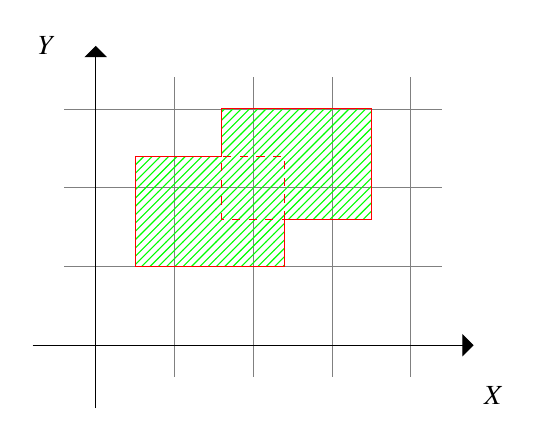
\begin{tikzpicture}[scale=2]
\draw[step=.5cm,gray,very thin] (-0.2,-0.2) grid (2.2,1.7);
\draw [-triangle 90] (-0.4,0) -- (2.4,0);
\draw [-triangle 90] (0,-0.4) -- (0,1.9); 
\draw (-0.2,1.9) node [anchor=east] {$Y$};
\draw (2.4,-0.2) node [anchor=north west] {$X$};
\filldraw [pattern=north east lines,pattern color = green,draw=red]  (0.8,1.5) -- (1.75,1.5) -- (1.75,0.8) -- (1.2,0.8) -- (1.2,0.5) -- (0.25,0.5) -- (0.25,1.2) -- (0.8,1.2) --cycle;
\draw [dashed,red] (1.2,0.8) rectangle (0.8,1.2);
\end{tikzpicture} 
\caption{}
\end{figure}
\end{enumerate}
\underline{Erinnerung:} Eine \emph{Äquivalenzrelation} auf einer Menge $ X $ ist eine Relation $\sim$ mit folgenden Eigenschaften:
\begin{enumerate}[(i)]
\item reflexiv: $a\sim a$
\item symmetrisch: $a\sim b \implies b\sim a$
\item transitiv: $a\sim b \land b \sim c\implies a\sim c$
\end{enumerate}
ist auf einer Menge $ X $ eine Äquivalenzrelation $\sim$ gegeben, so liegt jedes Element in seiner Äquivalenklasse
\[
 [x]:=\{y\in X|x\sim y\} \subset X
\]
und Äquivalenzklassen von zwei verschiedenen Elemente sind entweder disjunkt oder gleich; M zerfällt in die disjunkte Vereinigung der Äquivalenzklassen.  Umgekehrt liefert eine Zerlegung einer Menge in disjunkte Teilmengen eine Äquivalenzrelation.
\end{note*}
\begin{df}
Sei X ein topologischer Raum und $\sim$ eine Äquivalenzrelation auf $ X $.  Sei $X/\sim$ die Menge der Äquivalenzklassen 
\[
X/\sim=\{[x]|x\in X\}
\]
und sei $ q: X\to X/\sim, x\mapsto [x] $. Eine Teilmenge $ U $ von $ X/\sim $ ist genau dann offen bezüglich der \emph{Quotiententopologie} auf $ X/\sim $, wenn ihr Urbild $ q^{-1}(U) $ offen in X ist.
\end{df}

\begin{ex*}
\begin{enumerate}[(i)]
\item \begin{seg}{Zusammenschlagen eines Teilraums zu einem Punkt}
Sei $ X $ ein topologischer Raum und $ A\subset X $ ein Teilraum. Dann ist durch $ x \sim y :\equiv (x=y)\lor (x,y\in A) $ eine Äquivalenzrelation gegeben.  Zwei Punkte werden als äquivalent angesehen, wenn sie gleich sind oder beide in $ A $ liegen.
\end{seg}
\item \begin{seg}{Beispiel zu (i)}
Sei X ein topologischer Raum. Betrachte $ X\times [0,1] $
\begin{figure}[H]
\centering
 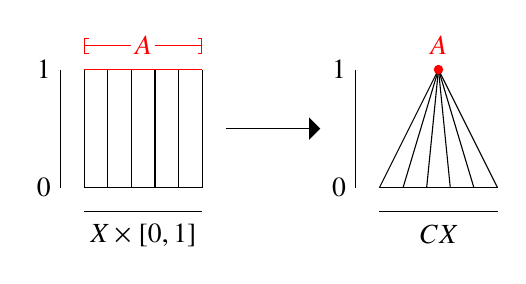
\begin{tikzpicture}[scale=1.5, >=triangle 90]
\begin {scope}
  \draw [-] (0,0) -- (0,1);
  \draw (0,0) node [anchor=east] {$0$};
  \draw (0,1) node [anchor=east] {$1$};
  \draw [-] (0.2,-0.2) -- (1.2,-0.2);
  \draw [-] (0.2,0) -- (1.2,0); 
  \draw [-,red] (0.2,1) -- (1.2,1);
  \draw [-] (0.2,0) -- (0.2,1);
  \draw [-] (0.4,0) -- (0.4,1);
  \draw [-] (0.6,0) -- (0.6,1);
  \draw [-] (0.8,0) -- (0.8,1);
  \draw [-] (1.0,0) -- (1.0,1);
  \draw [-] (1.2,0) -- (1.2,1);
  \draw [[-,red] (0.2,1.2) -- (0.6,1.2);
  \draw [-{]},red] (0.8,1.2) -- (1.2,1.2);
  \draw [red] (0.7,1.2) node [anchor=center] {$A$};
  \draw (0.7,-0.4) node [anchor=center] {$X \times [0,1]$};
\end {scope}
 \draw [->] (1.4,0.5) -- (2.2,0.5);
\begin {scope}[xshift=2.5cm,]
  \draw [-] (0,0) -- (0,1);
  \draw (0,0) node [anchor=east] {$0$};
  \draw (0,1) node [anchor=east] {$1$};
  \draw [-] (0.2,-0.2) -- (1.2,-0.2);
  \draw [-] (0.2,0) -- (1.2,0); 
  \draw [-] (0.2,0) -- (0.7,1);
  \draw [-] (0.4,0) -- (0.7,1);
  \draw [-] (0.6,0) -- (0.7,1);
  \draw [-] (0.8,0) -- (0.7,1);
  \draw [-] (1.0,0) -- (0.7,1);
  \draw [-] (1.2,0) -- (0.7,1);
  \filldraw [red] (0.7,1) circle (1pt);
  \draw [red] (0.7,1.2) node [anchor=center] {$A$};
  \draw (0.7,-0.4) node [anchor=center] {$CX$};
\end {scope}


\end{tikzpicture}
 



\caption{}
\end{figure}
Man erhält den Kegel $CX:=X\times[0,1]/X\times\{1\}$
\end{seg}
\item Allgemeiner: "`\emph{Zusammenkleben}"'
\begin{enumerate}[(a)]
\item .
\begin{figure}[H]
\centering
 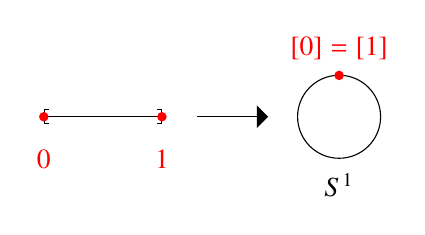
\begin{tikzpicture}[scale=1.5, >=triangle 90]
  \draw [[-{]}] (0,0) -- (1,0);
  \draw [red](0,-0.2) node [anchor=north] {$0$};
  \draw [red] (1,-0.2) node [anchor=north] {$1$};
  \draw [->] (1.3,0) -- (1.9,0);
  \draw (2.5,0) circle (10pt);
  \filldraw [red] (0,0) circle (1pt);
  \filldraw [red] (1,0) circle (1pt);
  \filldraw [red] (2.5,0.35) circle (1pt);
  \draw (2.5,-0.4) node [anchor=north] {$S^1$};
  \draw [red] (2.5,0.4) node [anchor=south] {$[0]=[1]$};
\end{tikzpicture}


\caption{}
\end{figure}
\item .
\begin{figure}[H]
\centering
 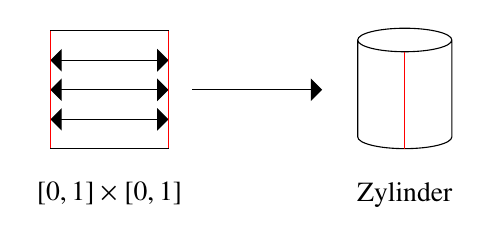
\begin{tikzpicture}[scale=1.5, >=triangle 90]
 \begin {scope}
  \draw [<->] (0,0.25) -- (1,0.25);
  \draw [<->] (0,0.5) -- (1,0.5);
  \draw [<->] (0,0.75) -- (1,0.75);
  \draw [-,red] (0,0) -- (0,1);
  \draw [-,red] (1,0) -- (1,1);
  \draw [-] (0,0) -- (1,0);
  \draw [-] (0,1) -- (1,1);
  \draw  (0.5,-0.2) node [anchor=north] {$[0,1] \times [0,1]$};
 \end {scope}
  \draw [->] (1.2,0.5) -- (2.3,0.5);
\begin {scope} [xshift=3cm,yshift=0.4cm]
  \node [cylinder,draw,rotate=90,scale=5.1,aspect=0.25] at (0,0){}; 
  \draw [-,red] (0,-0.4) -- (0,0.42);
  \draw  (0,-0.6) node [anchor=north] {Zylinder};
\end {scope}
\end{tikzpicture}

\caption{}
\end{figure}
\end{enumerate}
Bei (b) handelt es sich nicht um Zusammenschlagen eines Teilraums zu einem Punkt, sondern gegenüberliegende Punkte in den beiden senkrechten "`Randintervallen"' werden identifiziert mit der Äquivalenzrelation: \fixme[nachschauen]
\[
(x_1,x_2)\sim (y_1,y_2):\equiv (x_1,x_2)=(y_1,y_2)\lor (x_1,y_1 \in \{0,1\} \land x_2 =y_2)
\]
\end{enumerate}
\end{ex*}
Eine weitere Möglichkeit aus gegebenen topologischen Räumen andere zu konstruieren, ist es, Topologien mit Hilfe von Abbildungen zu übertragen.
\begin{df}\label{thm:2.5}
\begin{enumerate}[(i)]
\item Sei $ X $ ein topologischer Raum und $ Y $ eine Menge.  Sei $ f: X\to Y$ eine Abbildung.  Dann ist durch:
\[
\{U\subset Y|f^{-1}(U) \text{ offen} \}
\]
die \emph{finale Topologie} auf Y definiert.
\item Sei $ X $ eine Menge und $ X $ ein topologischer Raum.  Sei $ f: X\to Y $ eine Abbildung.  Dann ist durch 
\[
\{ f^{-1}(U)\subset X| U \text{ offen in } Y\}
\]
die \emph{initiale Topologie} auf X definiert.
\end{enumerate}
\end{df}
\begin{note*}
Die \emph{finale Topologie} ist die feinste Topologie auf Y die f stetig macht in (i). In (ii) ist die initiale Topologie die gröbste Topologie auf $ X $, die f stetig macht.
\end{note*}
\begin{exs*}
\begin{enumerate}[(i)]
\item Die Teilraumtopologie auf $M\subset X$ ist die initale Topologie bezüglich der \emph{Inklusionsabbildung} $ i:M\to X,m\mapsto m $, denn es gilt $ i^{-1}(U)=U\cap M $ für (offene) Mengen in $ X $.
\item Die Quotiententopologie ist die finale Topologie bezüglich der Quotientenabbildung  $ q: X\to X/\sim, x\mapsto [x] $
\item In ähnlicher Weise lässt sich die Summentopologie charakterisieren.  Sie ist die feinste Topologie, so dass beide Inklusionsabbildungen
$ i_X:X\to X+Y, x \mapsto x, i_Y: Y\to X+Y,y\mapsto y $ stetig sind.  Dies zeigt, dass es sinnvoll ist die Defnition \ref{thm:2.5} noch etwas weiter zu fassen.
\end{enumerate}
\end{exs*}
\begin{seg}{Zusatz zu Definition \ref{thm:2.5}}
Allgemeiner definieren wir:
\begin{enumerate}[(i)]
\setcounter{enumi}{2}
\item Seien $X_i, i\in I$ topologische Räume und $ Y $ eine Menge. Sei durch $f_i:X_i\to Y, i\in I$ eine Familie von Abbildungen gegeben. Die feinste Topologie auf $ Y $, die alle Abbildungen $f_i$ stetig macht, heißt finale Topologie bezüglich $ f_i,i\in I $.
\[
\{U\subset Y|f^{-1}_i(U) \text{ offen in }X_i \text{ \emph{für alle} } i\in I\}
\]
$(T1) U_1, U_2\in O$ zeige: $U_1\cup U_2\in O$
\[f^{-1}_i(U_1\cup U_2)=\underbrace{f^{-1}_i(U_1)}_{\text{offen in } X_i}\cup \underbrace{f^{-1}_i(U_2)}_{\text{offen in } X_i}\]
\item Seien $ Y_i, i\in I $, topologische Räume und $ X $ eine Menge.  Seien $ f_i: X\to Y_i $ Abbildungen.  Die gröbste Topologie auf $ X $, die alle $f_i$ stetig macht, ist die \emph{initiale Topologie} bezüglich $f_i$. 
\end{enumerate}
\end{seg}
\begin{ex*}
Die Produkttopologie auf $ X\times Y $ ist initiale Topologie bezüglich der beiden kanonischen Projektionen
\[
\pi_X:X\times Y \to X, (x,y)\mapsto x \text{ und } \pi_Y: X\times Y\to Y, (x,y)\mapsto y 
\]
\end{ex*}
\begin{seg}{Erläuterung zu Definition \ref{thm:2.5} (iv)} 
Ist eine Familie $ S $ von offenen Teilmengen auf einer Menge $ X $ gegeben, so erhalten wir dadurch den \emph{Hüllenoperator} 
\[ 
\mathcal T(S):=\bigcap\limits_{ O \text{ Topologie auf } X \text{ mit } S\subset O} O 
\]
Die gröbste Topologie auf $ X $, die alle Mengen in $ S $ enthält. Die Topologie $ \mathcal T(S) $ nennt man auch die \emph{von $ S $ erzeugte Topologie} auf $ X $.
\end{seg}
Die in (iv) definierte Topologie ist also durch
\[
\mathcal T(\bigcup\limits_{i\in I} \{ {f_i}^{-1}(U)|U \text{ offen in } Y_i\} )
\]
gegeben.
\begin{ex}\label{thm:2.6} Sei $ \R $ mit Standardtopologie versehen. Wir definieren eine Äquivalenzklasse $ [x] $ einer reellen Zahl $ x $ als die Menge $x+\Z=\{x+k|k\in \Z\}$. Sei $ X=\R/\sim $ mit der Quotiententopologie versehen. Wir \emph{behaupten}: $ X $ ist homöomorph zu $ Y:=\{v\in \R^2|\, ||v||=1\} $, dem Einheitskreis in $ \R^2 $, mit der Teilraumtopologie versehen. 
\begin{figure}[H]
\centering
\begin{tikzpicture}[scale=1.5, >=triangle 90]
  \draw [-] (-0.2,0) -- (5.2,0);
  \filldraw [red] (0,0) circle (1pt);
  \filldraw [red] (1,0) circle (1pt);
  \filldraw [red] (2,0) circle (1pt);
  \filldraw [red] (3,0) circle (1pt);
  \filldraw [red] (4,0) circle (1pt);
  \filldraw [red] (5,0) circle (1pt);
  \draw [red] (2,0) node [anchor=north] {x};  
\end{tikzpicture}


\caption{}
\end{figure}
\begin{proof}
Betrachte $ \phi(t)=(\cos(2\pi\cdot t),\sin(2\pi \cdot t)), \R\to Y $.
Wegen $ \phi(t+k)=\phi(t) $ für $ k\in \Z $, ist durch $ \bar\phi: X\to Y, [x]\mapsto \phi(x) $ eine wohldefinierte Abbildung gegeben. $\bar \phi$ ist offensichtlich bijektiv. Die Abbildung $ \bar \phi  $ ist stetig nach Definition der Quotientenabbildung, da $ \phi $ stetig ist.

Es bleibt noch zu zeigen: Die Bilder offener Mengen sind offen (man sagt dann: $ \bar \phi $ ist \emph{offen}, dass heißt die Bilder offener Mengen sind offen), dass heißt $ \bar \phi^{-1} $ ist stetig. Wir zeigen: Die Bilder abgeschlossener Mengen sind abgeschlossen: Sei $ A\subset X $ abgeschlossen. Dann ist $ q^{-1}(A)\subset \R $ abgeschlossen (mit $ q: \R \to \R/\sim $ die Quotientenabbildung).

Es gilt $ \bar \phi(A)=\phi(q^{-1}(A))=\phi(q^{-1}(A)\cap[0,1]) $. Da $ q^{-1}(A)\cap [0,1] $ kompakte Teilmenge von $ \R $ ist, ist $ \bar\phi(A)=\phi(q^{-1}(A)\cap[0,1]) $ kompakt, also abgeschlossene Teilmenge des $ \R^2  $ und somit von $ Y $.
\end{proof}
\end{ex}
\subsection{Hausdorffräume}
\begin{df}[Hausdorffsches Trennungsaxiom]
 Ein topologischer Raum heißt \emph{Hausdorffraum}, wenn man zu je zwei verschiedenen Punkten disjunkte Umgebungen finden kann.
\begin{figure}[H]
\centering
 \fixme[fig13]
\caption{}
\end{figure}
\end{df}
\begin{st}
Jeder metrische Raum ist ein Hausdorffraum. 
\end{st}
\begin{proof}
Dies folgt aus der Dreiecksungleichung der Metrik. 
\begin{figure}[H]
\centering
 \fixme[fig14]
\caption{}
\end{figure}
Seien $x$ und $y$ Punkte im metrischen Raum und sei $d(x,y)>0$.
Dann sind die beiden $\eps$-Bälle $B_\eps(x)$ und $B_\eps(y)$ mit $\eps:=\frac{1}{2}d(x,y)$ disjunkte Umgebungen von $x$ bzw. $y$. Denn 
wäre $z\in B_\eps(x) \cap B_\eps(y)$, dann wäre die Dreiecksungleichung
\[
\underbrace{d(x,z)}_{<\eps}+\underbrace{d(z,y)}_{<\eps}\ge d(x,y)=2\eps
\]        
verletzt.
\end{proof}
\begin{st}
Jeder Teilraum eines Hausdorffraums ist Hausdorffsch. Zwei topologische Räume sind genau dann Hausdorffsch, wenn ihre topologische Summe es ist und zwei nichtleere topologische Räume sind Hausdorffsch, genau dann wenn ihr Produkt es ist. 
\end{st}
\begin{proof}[zur Übung]\end{proof}
\begin{note*}
die Quotiententopologie von Hausdorffräumen sind nicht notwendigerweise hausdorffsch, siehe dafür das folgendende Beispiel.
\begin{figure}[H]
\centering
 \fixme[fig15]
\caption{}
\end{figure}
\end{note*}
Ein Raum, der nicht Hausdorffsch ist, scheint mit unserer Intuition unvereinbar zu sein.  Ein typisches Beispiel ist die Klumpentopologie $\{\emptyset, X\}$ auf jeder Menge. Mit Hilfe der Quotiententopologie erhält man weniger triviale Beispiele von Nicht-Hausdorffräumen.
\begin{ex*} Für Nicht-Hausdorffraum:\\
Die Gerade mit einem Doppelpunkt. Sei $ X=\R+\R=\R\times \{0\}\cup \R\times \{1\} $. Definiere man $ (x,n)\sim (y,m)\stackrel{\text{def}}{\iff} x=y\neq 0 $. \\
\begin{figure}[H]
\centering
 \begin{tikzpicture}[scale=1.5, >=triangle 90]
\begin {scope}
 \draw [-] (-0.2,0) -- (5.2,0);
  \draw  (5.4,0) node [anchor=west] {$\R \times \{1\}$};  
  \draw [-] (-0.2,-1) -- (5.2,-1);
  \draw  (5.4,-1) node [anchor=west] {$\R \times \{0\}$};  
  \filldraw [red] (2.5,0) circle (1pt);
  \filldraw [red] (2.5,-1) circle (1pt);
  \draw [red] (2.5,0) node [anchor=north] {$(0,1)$};  
  \draw [red] (2.5,-1) node [anchor=north] {$(0,0)$};  
  \draw [<->] (0,-0.1) -- (0,-0.9);
  \draw [<->] (1,-0.1) -- (1,-0.9);
  \draw [<->] (2,-0.1) -- (2,-0.9);
  \draw [<->] (3,-0.1) -- (3,-0.9);
  \draw [<->] (4,-0.1) -- (4,-0.9);
  \draw [<->] (5,-0.1) -- (5,-0.9);
\end {scope}
  \draw [->] (2.5,-1.6) -- (2.5,-2.5);
\begin {scope} [yshift=-0.3cm]
  \draw [-] (-0.2,-3) -- (2.3,-3);
  \draw [-] ( 2.7,-3) -- (5.2,-3);
  \draw [red] (2.5,-2.8) node [anchor=south] {$[(0,1)]$};  
  \filldraw [red] (2.5,-2.8) circle (1pt);
  \filldraw [red] (2.5,-3.2) circle (1pt);
  \draw [red] (2.5,-3.2) node [anchor=north] {$[(0,0)]$};  
  \draw  (5.4,-3) node [anchor=west] {$(\R + \R) / \sim$};  
\end {scope}  
\end{tikzpicture}


\caption{}
\end{figure}
$ \R $ besitzt unter Betrachtung dieser Relation doppelt vorhandene Nullpunkte.
\begin{figure}[H]
\centering
 \fixme[fig17]
\caption{}
\end{figure}
Die beiden Punkte $[(0,0)]$ und $[(0,1)]$ in $ X/\sim $ lassen sich nicht durch disjunkte Umgebung trennen.\\
\begin{figure}[H]
\centering
 \fixme[fig18]
\caption{}
\end{figure}
\end{ex*}
Wir wollen noch zwei weitere Eigenschaften von Hausdorffräumen beweisen, die mit der geometrischen Intuition übereinstimmen.
\begin{st}
In einem Hausdorffraum gilt:
\begin{enumerate}[(i)]
\item Der Limes einer konvergenten Folge ist eindeutig bestimmt.
\item Punkte sind abgeschlossen.
\end{enumerate}
\end{st}
\begin{proof}
\begin{enumerate}[(i)]
\item Seien $ a\neq b $ verschiedene Limiten einer konvergenten Folge $ x_n $, dann gibt es disjunkte Umgebungen $ U_a $ und $ U_b $ von $ a $ bzw. $ b $.  Da $ x_n $ gegen $ a $ konvergiert, liegen fast alle Folgenglieder in $ U_a $, im Widerspruch zur Konvergenz von $ x_n $ gegen $ b $.
\item Das Komplement einer einelementigen Menge ist offen, denn nach der Hausdorffeigenschaft gibt es um jeden ihrer Punkte eine Umgebung, die insbesondere p nicht enthält.
\end{enumerate}
\end{proof}
\begin{note*}
Dies liefert eine notwendige Bedingung dafür, dass eine Quotiententopologie Hausdorffsch ist.  Alle Äquivalenzklassen müssen abgeschlossen sein.
\end{note*}
\subsection{Zusammenhang und Wegzusammenhang}
\begin{df}
Ein topologischer Raum heißt \emph{zusammmenhängend}, wenn er sich nicht in zwei nichtleere, offene, disjunkte Teilmengen zerlegen lässt.
\end{df}
\begin{figure}[H]
\centering
  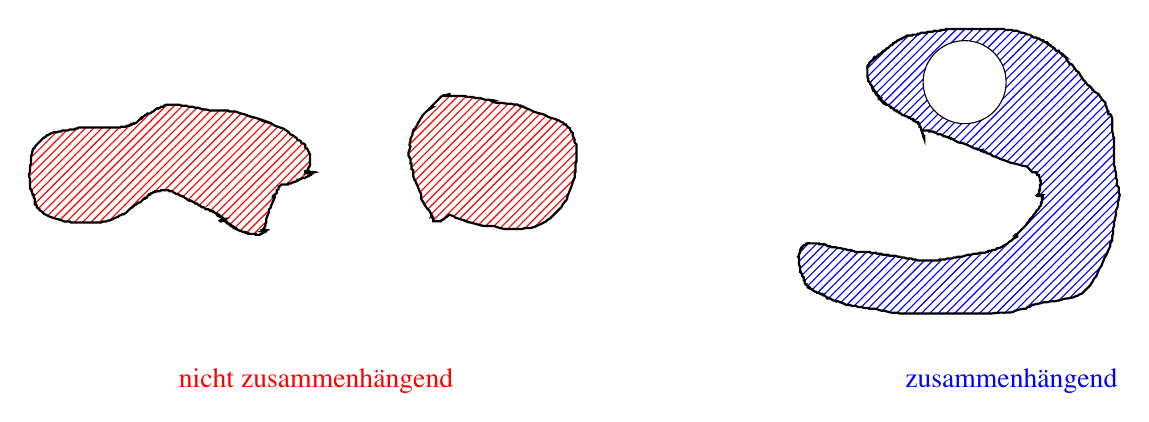
\begin{tikzpicture}[y=0.80pt,x=0.80pt,yscale=-1,scale=0.3, inner sep=0pt, outer sep=0pt]
  \draw [red] (230,800) node [anchor=east] {nicht zusammenhängend};
  \draw [blue] (1230,800) node [anchor=east] {zusammenhängend};
  
   \path[draw=black,fill,pattern color = red,pattern=north east lines,line join=miter,line cap=butt,line width=0.800pt]
    (224.2857,549.5050) .. controls (226.6667,550.4574) and (229.1349,551.2154) ..
    (231.4286,552.3622) .. controls (232.0309,552.6633) and (232.2548,553.4896) ..
    (232.8571,553.7908) .. controls (234.2040,554.4642) and (235.7143,554.7431) ..
    (237.1429,555.2193) .. controls (238.5714,555.6955) and (239.9807,556.2342) ..
    (241.4286,556.6479) .. controls (243.3164,557.1873) and (245.3045,557.3871) ..
    (247.1429,558.0765) .. controls (266.1534,565.2054) and (238.0850,556.8834) ..
    (260.0000,562.3622) .. controls (267.4477,564.2241) and (271.0400,566.1458) ..
    (278.5714,566.6479) .. controls (282.8477,566.9330) and (287.1805,566.0815) ..
    (291.4286,566.6479) .. controls (297.7954,568.7702) and (300.6814,570.1259) ..
    (307.1429,570.9336) .. controls (308.5604,571.1108) and (310.0000,570.9336) ..
    (311.4286,570.9336) .. controls (315.2381,570.9336) and (319.0476,570.9336) ..
    (322.8571,570.9336) .. controls (325.7143,570.9336) and (328.5714,570.9336) ..
    (331.4286,570.9336) .. controls (332.3810,570.9336) and (333.3618,571.1646) ..
    (334.2857,570.9336) .. controls (335.7466,570.5684) and (337.0948,569.8004) ..
    (338.5714,569.5050) .. controls (339.9891,569.2215) and (344.2134,569.5050) ..
    (345.7143,569.5050) .. controls (346.1905,569.5050) and (346.6809,569.6205) ..
    (347.1429,569.5050) .. controls (353.2774,567.9714) and (358.6871,565.1615) ..
    (364.2857,562.3622) .. controls (365.2381,561.8860) and (366.1905,561.4098) ..
    (367.1429,560.9336) .. controls (368.0952,560.4574) and (369.1482,560.1439) ..
    (370.0000,559.5050) .. controls (371.0775,558.6969) and (371.7797,557.4560) ..
    (372.8571,556.6479) .. controls (373.7090,556.0090) and (374.8625,555.8582) ..
    (375.7143,555.2193) .. controls (376.7918,554.4112) and (377.6191,553.3146) ..
    (378.5714,552.3622) .. controls (380.4762,550.4574) and (382.3810,548.5527) ..
    (384.2857,546.6479) .. controls (385.7143,545.2193) and (387.1429,543.7907) ..
    (388.5714,542.3622) .. controls (390.0000,540.9336) and (391.5951,539.6541) ..
    (392.8571,538.0765) .. controls (393.5223,537.2450) and (393.8095,536.1717) ..
    (394.2857,535.2193) .. controls (395.2381,533.7907) and (396.0703,532.2743) ..
    (397.1429,530.9336) .. controls (397.9842,529.8819) and (399.1919,529.1540) ..
    (400.0000,528.0765) .. controls (403.3219,523.6473) and (400.6771,526.7967) ..
    (401.4286,523.7908) .. controls (401.7938,522.3299) and (402.2979,520.9032) ..
    (402.8571,519.5050) .. controls (403.2526,518.5164) and (403.8903,517.6365) ..
    (404.2857,516.6479) .. controls (404.8450,515.2498) and (405.1550,513.7603) ..
    (405.7143,512.3622) .. controls (406.1097,511.3736) and (406.7474,510.4937) ..
    (407.1429,509.5050) .. controls (408.8177,505.3179) and (409.7537,500.8351) ..
    (411.4286,496.6479) .. controls (411.8240,495.6593) and (412.5989,494.8238) ..
    (412.8571,493.7908) .. controls (413.4174,491.5499) and (412.2969,488.8888) ..
    (412.8571,486.6479) .. controls (413.0205,485.9946) and (414.0728,485.8582) ..
    (414.2857,485.2193) .. controls (414.5869,484.3158) and (414.2857,483.3146) ..
    (414.2857,482.3622) .. controls (414.2857,480.9336) and (414.2857,479.5050) ..
    (414.2857,478.0765) .. controls (414.2857,476.8385) and (414.0099,473.1897) ..
    (414.2857,472.3622) .. controls (414.6224,471.3520) and (415.4560,470.5380) ..
    (415.7143,469.5050) .. controls (415.9859,468.4187) and (415.7143,463.5585) ..
    (415.7143,462.3622) .. controls (415.7143,458.5527) and (415.7143,454.7431) ..
    (415.7143,450.9336) .. controls (415.7143,450.1261) and (416.0273,444.2602) ..
    (415.7143,443.7908) .. controls (414.9672,442.6701) and (413.4595,442.1383) ..
    (412.8571,440.9336) .. controls (411.4286,438.0765) and (413.5714,438.7908) ..
    (412.8571,436.6479) .. controls (412.1837,434.6276) and (410.6734,432.9539) ..
    (410.0000,430.9336) .. controls (409.6838,429.9849) and (410.3162,427.5966) ..
    (410.0000,426.6479) .. controls (409.5741,425.3701) and (407.8900,424.9114) ..
    (407.1429,423.7908) .. controls (406.5522,422.9048) and (406.0510,421.9438) ..
    (405.7143,420.9336) .. controls (405.5637,420.4819) and (406.0510,419.8418) ..
    (405.7143,419.5050) .. controls (402.2446,416.0353) and (403.6165,419.9299) ..
    (401.4286,416.6479) .. controls (400.8379,415.7619) and (400.8860,414.3814) ..
    (400.0000,413.7908) .. controls (399.2076,413.2625) and (397.9353,414.3190) ..
    (397.1429,413.7908) .. controls (396.2569,413.2001) and (396.5661,411.5725) ..
    (395.7143,410.9336) .. controls (394.5096,410.0301) and (392.7754,410.1785) ..
    (391.4286,409.5050) .. controls (390.8262,409.2039) and (390.6023,408.3776) ..
    (390.0000,408.0765) .. controls (388.6531,407.4030) and (387.1124,407.2072) ..
    (385.7143,406.6479) .. controls (384.7256,406.2524) and (383.8673,405.5560) ..
    (382.8571,405.2193) .. controls (380.1108,404.3039) and (375.6087,403.7380) ..
    (372.8571,402.3622) .. controls (371.3215,401.5944) and (370.1071,400.2729) ..
    (368.5714,399.5050) .. controls (366.1709,398.3048) and (360.8600,397.3345) ..
    (358.5714,396.6479) .. controls (344.1197,392.3124) and (355.4231,395.7068) ..
    (344.2857,390.9336) .. controls (341.0333,389.5397) and (339.9020,389.9159) ..
    (337.1429,388.0765) .. controls (336.5825,387.7029) and (336.3676,386.8112) ..
    (335.7143,386.6479) .. controls (334.3284,386.3014) and (332.7838,387.0997) ..
    (331.4286,386.6479) .. controls (330.9768,386.4973) and (331.8545,385.4323) ..
    (331.4286,385.2193) .. controls (330.5767,384.7934) and (329.4749,385.5205) ..
    (328.5714,385.2193) .. controls (327.9325,385.0064) and (327.7817,384.0037) ..
    (327.1429,383.7908) .. controls (325.3358,383.1884) and (323.2963,384.1643) ..
    (321.4286,383.7908) .. controls (319.9520,383.4954) and (318.6371,382.5490) ..
    (317.1429,382.3622) .. controls (314.7803,382.0669) and (312.3712,382.5777) ..
    (310.0000,382.3622) .. controls (307.1153,382.0999) and (304.3132,381.1959) ..
    (301.4286,380.9336) .. controls (299.0574,380.7181) and (296.5956,381.5111) ..
    (294.2857,380.9336) .. controls (275.0888,376.1344) and (306.8492,379.4683) ..
    (284.2857,376.6479) .. controls (282.3957,376.4116) and (280.4392,377.0215) ..
    (278.5714,376.6479) .. controls (275.6182,376.0573) and (272.9218,374.5212) ..
    (270.0000,373.7908) .. controls (267.6901,373.2133) and (265.1919,374.2577) ..
    (262.8571,373.7908) .. controls (261.8130,373.5819) and (261.0441,372.5710) ..
    (260.0000,372.3622) .. controls (257.1983,371.8019) and (254.2302,372.9225) ..
    (251.4286,372.3622) .. controls (250.3844,372.1534) and (249.6044,371.1919) ..
    (248.5714,370.9336) .. controls (247.6475,370.7026) and (246.6667,370.9336) ..
    (245.7143,370.9336) .. controls (243.8095,370.9336) and (241.9048,370.9336) ..
    (240.0000,370.9336) .. controls (234.7619,370.9336) and (229.5238,370.9336) ..
    (224.2857,370.9336) .. controls (223.3333,370.9336) and (222.3809,370.9336) ..
    (221.4286,370.9336) .. controls (220.9524,370.9336) and (219.5741,371.1466) ..
    (220.0000,370.9336) .. controls (221.3469,370.2602) and (223.0328,370.3403) ..
    (224.2857,369.5050) .. controls (224.6819,369.2409) and (224.7619,368.0765) ..
    (224.2857,368.0765) .. controls (222.3223,368.0765) and (220.4967,369.1200) ..
    (218.5714,369.5050) .. controls (217.6375,369.6918) and (216.5661,369.0791) ..
    (215.7143,369.5050) .. controls (215.1119,369.8062) and (214.8880,370.6324) ..
    (214.2857,370.9336) .. controls (213.8598,371.1466) and (213.2831,370.7207) ..
    (212.8571,370.9336) .. controls (212.0942,371.3151) and (209.3235,374.4672) ..
    (208.5714,375.2193) .. controls (205.7143,378.0765) and (202.8571,380.9336) ..
    (200.0000,383.7908) .. controls (199.5238,384.2669) and (199.0476,384.7431) ..
    (198.5714,385.2193) .. controls (197.6190,386.1717) and (195.7143,386.7296) ..
    (195.7143,388.0765) .. controls (195.7143,389.0289) and (199.2449,387.4030) ..
    (198.5714,388.0765) .. controls (196.6080,390.0399) and (193.7389,390.8220) ..
    (191.4286,392.3622) .. controls (190.8682,392.7357) and (190.4762,393.3146) ..
    (190.0000,393.7908) .. controls (189.0476,394.7431) and (188.0952,395.6955) ..
    (187.1429,396.6479) .. controls (186.1905,397.6003) and (185.0328,398.3844) ..
    (184.2857,399.5050) .. controls (183.6951,400.3910) and (183.4478,401.4762) ..
    (182.8571,402.3622) .. controls (182.4836,402.9225) and (181.8021,403.2304) ..
    (181.4286,403.7908) .. controls (180.2473,405.5627) and (179.7527,407.7331) ..
    (178.5714,409.5050) .. controls (178.1979,410.0654) and (177.4440,410.3313) ..
    (177.1429,410.9336) .. controls (176.4694,412.2805) and (176.3877,413.8725) ..
    (175.7143,415.2193) .. controls (175.4131,415.8217) and (174.6593,416.0876) ..
    (174.2857,416.6479) .. controls (173.6951,417.5339) and (173.3333,418.5527) ..
    (172.8571,419.5050) .. controls (171.9048,420.4574) and (170.7471,421.2415) ..
    (170.0000,422.3622) .. controls (169.7359,422.7584) and (170.1506,423.3390) ..
    (170.0000,423.7908) .. controls (169.6633,424.8009) and (168.8297,425.6149) ..
    (168.5714,426.6479) .. controls (168.3404,427.5718) and (168.8726,428.6015) ..
    (168.5714,429.5050) .. controls (167.8980,431.5253) and (166.3877,433.1990) ..
    (165.7143,435.2193) .. controls (165.4131,436.1228) and (165.9011,437.1426) ..
    (165.7143,438.0765) .. controls (165.2793,440.2514) and (163.4668,442.7627) ..
    (164.2857,445.2193) .. controls (164.4987,445.8582) and (165.7143,445.9745) ..
    (165.7143,446.6479) .. controls (165.7143,448.1537) and (164.6509,449.4727) ..
    (164.2857,450.9336) .. controls (164.1702,451.3956) and (164.4363,451.9104) ..
    (164.2857,452.3622) .. controls (163.9490,453.3723) and (163.1154,454.1863) ..
    (162.8571,455.2193) .. controls (162.5107,456.6052) and (162.8571,458.0765) ..
    (162.8571,459.5050) .. controls (162.8571,459.9812) and (162.6442,460.5077) ..
    (162.8571,460.9336) .. controls (163.1583,461.5360) and (163.9845,461.7598) ..
    (164.2857,462.3622) .. controls (164.4987,462.7881) and (164.0728,463.3648) ..
    (164.2857,463.7908) .. controls (164.5869,464.3931) and (165.4131,464.6170) ..
    (165.7143,465.2193) .. controls (166.2077,466.2061) and (165.2128,471.8607) ..
    (165.7143,472.3622) .. controls (166.0510,472.6989) and (166.8061,472.0255) ..
    (167.1429,472.3622) .. controls (167.1888,472.4082) and (167.1429,476.3014) ..
    (167.1429,476.6479) .. controls (167.1429,477.1241) and (167.1429,477.6003) ..
    (167.1429,478.0765) .. controls (167.1429,479.0289) and (166.6146,480.1412) ..
    (167.1429,480.9336) .. controls (167.7335,481.8196) and (169.2471,481.6093) ..
    (170.0000,482.3622) .. controls (170.3367,482.6989) and (170.0000,483.3146) ..
    (170.0000,483.7908) .. controls (170.0000,485.1749) and (169.7161,491.5104) ..
    (170.0000,492.3622) .. controls (170.3367,493.3723) and (171.0918,494.2092) ..
    (171.4286,495.2193) .. controls (171.5792,495.6711) and (171.2156,496.2220) ..
    (171.4286,496.6479) .. controls (171.7297,497.2502) and (172.5560,497.4741) ..
    (172.8571,498.0765) .. controls (174.0040,500.3701) and (174.7041,502.8623) ..
    (175.7143,505.2193) .. controls (176.1337,506.1980) and (176.7474,507.0878) ..
    (177.1429,508.0765) .. controls (177.7021,509.4746) and (177.9782,510.9781) ..
    (178.5714,512.3622) .. controls (179.4103,514.3196) and (180.9666,515.9976) ..
    (181.4286,518.0765) .. controls (183.2352,526.2064) and (179.5558,523.1245) ..
    (182.8571,528.0765) .. controls (183.2307,528.6368) and (183.9122,528.9447) ..
    (184.2857,529.5050) .. controls (185.4670,531.2770) and (185.9616,533.4474) ..
    (187.1429,535.2193) .. controls (187.5164,535.7797) and (188.1979,536.0876) ..
    (188.5714,536.6479) .. controls (189.1621,537.5339) and (189.4094,538.6191) ..
    (190.0000,539.5050) .. controls (191.0989,541.1534) and (193.1868,542.1424) ..
    (194.2857,543.7908) .. controls (194.8764,544.6767) and (195.1236,545.7619) ..
    (195.7143,546.6479) .. controls (196.0878,547.2082) and (196.9299,547.4376) ..
    (197.1429,548.0765) .. controls (197.1429,556.1717) and (196.1905,548.5527) ..
    (198.5714,550.9336) .. controls (199.2449,551.6071) and (197.8980,553.1173) ..
    (198.5714,553.7908) .. controls (198.9082,554.1275) and (199.6633,553.4540) ..
    (200.0000,553.7908) .. controls (200.3438,554.1345) and (199.6562,559.1613) ..
    (200.0000,559.5050) .. controls (200.0459,559.5509) and (203.9392,559.5050) ..
    (204.2857,559.5050) .. controls (204.9593,559.5050) and (211.3638,559.5697) ..
    (211.4286,559.5050) .. controls (211.7653,559.1683) and (211.0918,558.4132) ..
    (211.4286,558.0765) .. controls (211.7653,557.7398) and (212.4312,558.2894) ..
    (212.8571,558.0765) .. controls (213.4595,557.7753) and (213.6834,556.9491) ..
    (214.2857,556.6479) .. controls (214.7116,556.4349) and (215.2884,556.8609) ..
    (215.7143,556.6479) .. controls (216.3166,556.3467) and (216.6255,555.6505) ..
    (217.1429,555.2193) .. controls (219.4853,553.2673) and (221.9048,551.4098) ..
    (224.2857,549.5050) -- cycle;
  \path[draw=black,fill,pattern color = red,pattern=north east lines,line join=miter,line cap=butt,line width=0.800pt,xshift=-400pt,yshift=230pt]
    (220.0000,130.9336) .. controls (206.1905,130.9336) and (192.3809,130.9336) ..
    (178.5714,130.9336) .. controls (175.7143,130.9336) and (172.8571,130.9336) ..
    (170.0000,130.9336) .. controls (169.3566,130.9336) and (166.1490,130.7162) ..
    (165.7143,130.9336) .. controls (165.1120,131.2348) and (164.8880,132.0610) ..
    (164.2857,132.3622) .. controls (163.4339,132.7881) and (162.2804,131.9363) ..
    (161.4286,132.3622) .. controls (160.8262,132.6634) and (160.6389,133.5778) ..
    (160.0000,133.7908) .. controls (158.6766,134.2319) and (154.2260,133.3345) ..
    (152.8571,133.7908) .. controls (151.8470,134.1275) and (151.0101,134.8826) ..
    (150.0000,135.2193) .. controls (149.0744,135.5279) and (144.0267,135.2193) ..
    (142.8571,135.2193) .. controls (142.3809,135.2193) and (141.8545,135.0064) ..
    (141.4286,135.2193) .. controls (140.8262,135.5205) and (140.6389,136.4349) ..
    (140.0000,136.6479) .. controls (139.0965,136.9491) and (138.0952,136.6479) ..
    (137.1429,136.6479) .. controls (136.6667,136.6479) and (136.1402,136.4349) ..
    (135.7143,136.6479) .. controls (135.1119,136.9491) and (134.9246,137.8635) ..
    (134.2857,138.0765) .. controls (132.4787,138.6788) and (130.4193,137.6145) ..
    (128.5714,138.0765) .. controls (127.5384,138.3347) and (126.7244,139.1683) ..
    (125.7143,139.5050) .. controls (125.2625,139.6556) and (124.7116,139.2921) ..
    (124.2857,139.5050) .. controls (122.7500,140.2729) and (121.5357,141.5944) ..
    (120.0000,142.3622) .. controls (119.5741,142.5751) and (118.9676,142.0980) ..
    (118.5714,142.3622) .. controls (117.4508,143.1093) and (116.7918,144.4112) ..
    (115.7143,145.2193) .. controls (114.8624,145.8582) and (113.7431,146.0573) ..
    (112.8571,146.6479) .. controls (112.2968,147.0215) and (111.9048,147.6003) ..
    (111.4286,148.0765) .. controls (110.0000,149.5050) and (108.5714,150.9336) ..
    (107.1429,152.3622) .. controls (106.1905,153.3146) and (105.2381,154.2669) ..
    (104.2857,155.2193) .. controls (103.3333,156.1717) and (102.2367,156.9990) ..
    (101.4286,158.0765) .. controls (100.7897,158.9283) and (100.6389,160.0818) ..
    (100.0000,160.9336) .. controls (99.1919,162.0111) and (97.8900,162.6701) ..
    (97.1429,163.7907) .. controls (96.8787,164.1870) and (97.2934,164.7676) ..
    (97.1429,165.2193) .. controls (93.0959,173.3132) and (97.6753,163.0897) ..
    (95.7143,170.9336) .. controls (95.4560,171.9666) and (94.6224,172.7806) ..
    (94.2857,173.7907) .. controls (94.1351,174.2425) and (94.2857,174.7431) ..
    (94.2857,175.2193) .. controls (94.2857,177.6003) and (94.2857,179.9812) ..
    (94.2857,182.3622) .. controls (94.2857,183.3146) and (94.5167,184.2954) ..
    (94.2857,185.2193) .. controls (94.0275,186.2523) and (93.1154,187.0435) ..
    (92.8571,188.0765) .. controls (92.6262,189.0004) and (92.8571,189.9812) ..
    (92.8571,190.9336) .. controls (92.8571,192.1299) and (93.1287,196.9901) ..
    (92.8571,198.0765) .. controls (92.5989,199.1095) and (91.7653,199.9235) ..
    (91.4286,200.9336) .. controls (91.2780,201.3854) and (91.4286,201.8860) ..
    (91.4286,202.3622) .. controls (91.4286,207.9428) and (91.0027,202.5130) ..
    (92.8571,208.0765) .. controls (93.1258,208.8825) and (92.8571,211.4235) ..
    (92.8571,212.3622) .. controls (92.8571,214.7431) and (92.8571,217.1241) ..
    (92.8571,219.5050) .. controls (92.8571,219.9812) and (92.8571,220.4574) ..
    (92.8571,220.9336) .. controls (92.8571,221.4098) and (92.6442,221.9363) ..
    (92.8571,222.3622) .. controls (97.5951,227.1002) and (92.1837,221.0153) ..
    (94.2857,225.2193) .. controls (94.5869,225.8217) and (95.4131,226.0456) ..
    (95.7143,226.6479) .. controls (96.1402,227.4997) and (95.2884,228.6532) ..
    (95.7143,229.5050) .. controls (96.0155,230.1074) and (96.8417,230.3313) ..
    (97.1429,230.9336) .. controls (97.3558,231.3595) and (96.8061,232.0255) ..
    (97.1429,232.3622) .. controls (97.4796,232.6989) and (98.2347,232.0255) ..
    (98.5714,232.3622) .. controls (98.8635,232.6542) and (98.2882,236.0815) ..
    (98.5714,236.6479) .. controls (98.8726,237.2502) and (99.6988,237.4741) ..
    (100.0000,238.0765) .. controls (100.2583,238.5931) and (100.0000,244.2257) ..
    (100.0000,245.2193) .. controls (100.0000,245.6955) and (99.6633,246.3112) ..
    (100.0000,246.6479) .. controls (102.9558,249.6037) and (99.8845,242.1311) ..
    (102.8571,248.0765) .. controls (103.2831,248.9283) and (102.4312,250.0818) ..
    (102.8571,250.9336) .. controls (103.9511,253.1216) and (105.4029,252.0508) ..
    (107.1429,253.7908) .. controls (107.4796,254.1275) and (106.8061,254.8826) ..
    (107.1429,255.2193) .. controls (107.8958,255.9723) and (109.1140,256.0573) ..
    (110.0000,256.6479) .. controls (111.6810,257.7686) and (112.6695,259.7214) ..
    (114.2857,260.9336) .. controls (115.1375,261.5725) and (116.1905,261.8860) ..
    (117.1429,262.3622) .. controls (119.0476,263.3146) and (120.8799,264.4284) ..
    (122.8571,265.2193) .. controls (127.4990,267.0761) and (132.3579,268.1379) ..
    (137.1429,269.5050) .. controls (138.5908,269.9187) and (140.0304,270.3743) ..
    (141.4286,270.9336) .. controls (142.4172,271.3291) and (143.2416,272.1534) ..
    (144.2857,272.3622) .. controls (147.0874,272.9225) and (150.0853,271.6692) ..
    (152.8571,272.3622) .. controls (153.5105,272.5255) and (153.6834,273.4896) ..
    (154.2857,273.7907) .. controls (154.8958,274.0958) and (160.8638,273.7907) ..
    (161.4286,273.7907) .. controls (168.0952,273.7907) and (174.7619,273.7907) ..
    (181.4286,273.7907) .. controls (186.1905,273.7907) and (190.9524,273.7907) ..
    (195.7143,273.7907) .. controls (197.1429,273.7907) and (198.5992,274.0709) ..
    (200.0000,273.7907) .. controls (201.0441,273.5819) and (201.8241,272.6204) ..
    (202.8571,272.3622) .. controls (204.2431,272.0157) and (205.7876,272.8139) ..
    (207.1429,272.3622) .. controls (208.1530,272.0255) and (208.9898,271.2703) ..
    (210.0000,270.9336) .. controls (210.9035,270.6324) and (211.9536,271.2348) ..
    (212.8571,270.9336) .. controls (214.8774,270.2602) and (216.6667,269.0288) ..
    (218.5714,268.0765) .. controls (219.5238,267.6003) and (220.4399,267.0433) ..
    (221.4286,266.6479) .. controls (222.8267,266.0886) and (224.3674,265.8928) ..
    (225.7143,265.2193) .. controls (226.3166,264.9182) and (226.5825,264.1643) ..
    (227.1429,263.7907) .. controls (228.0288,263.2001) and (229.0476,262.8384) ..
    (230.0000,262.3622) .. controls (230.9524,261.8860) and (231.8470,261.2703) ..
    (232.8571,260.9336) .. controls (237.1098,259.5161) and (229.9260,264.3163) ..
    (237.1429,259.5050) .. controls (237.7032,259.1315) and (238.0952,258.5527) ..
    (238.5714,258.0765) .. controls (239.5238,257.1241) and (240.4762,256.1717) ..
    (241.4286,255.2193) .. controls (242.3809,254.2669) and (243.1650,253.1093) ..
    (244.2857,252.3622) .. controls (245.1717,251.7715) and (246.2569,251.5243) ..
    (247.1429,250.9336) .. controls (248.2635,250.1865) and (248.8793,248.8236) ..
    (250.0000,248.0765) .. controls (250.8860,247.4858) and (251.9712,247.2385) ..
    (252.8571,246.6479) .. controls (253.9778,245.9008) and (254.4365,244.2167) ..
    (255.7143,243.7908) .. controls (256.6178,243.4896) and (257.6679,244.0919) ..
    (258.5714,243.7908) .. controls (259.6554,243.4294) and (262.9728,238.7329) ..
    (264.2857,238.0765) .. controls (264.7116,237.8635) and (265.3776,238.4132) ..
    (265.7143,238.0765) .. controls (266.0510,237.7398) and (265.2884,236.8609) ..
    (265.7143,236.6479) .. controls (266.5661,236.2220) and (267.7790,237.1762) ..
    (268.5714,236.6479) .. controls (269.4574,236.0573) and (269.4094,234.6767) ..
    (270.0000,233.7908) .. controls (269.0426,231.7755) and (272.6804,232.5390) ..
    (272.8571,232.3622) .. controls (273.1939,232.0255) and (272.5204,231.2703) ..
    (272.8571,230.9336) .. controls (273.1939,230.5969) and (273.8598,231.1466) ..
    (274.2857,230.9336) .. controls (274.8880,230.6324) and (275.1119,229.8062) ..
    (275.7143,229.5050) .. controls (276.1402,229.2921) and (276.7169,229.7180) ..
    (277.1429,229.5050) .. controls (277.7452,229.2039) and (277.9691,228.3776) ..
    (278.5714,228.0765) .. controls (279.4233,227.6506) and (280.7551,228.7499) ..
    (281.4286,228.0765) .. controls (281.7653,227.7398) and (281.0026,226.8609) ..
    (281.4286,226.6479) .. controls (282.3053,226.2095) and (287.6858,227.0907) ..
    (288.5714,226.6479) .. controls (289.1738,226.3467) and (289.3977,225.5205) ..
    (290.0000,225.2193) .. controls (290.3202,225.0592) and (295.3748,225.2193) ..
    (295.7143,225.2193) .. controls (296.9238,225.2193) and (300.6606,224.9633) ..
    (301.4286,225.2193) .. controls (302.0674,225.4323) and (302.2548,226.3467) ..
    (302.8571,226.6479) .. controls (303.2831,226.8609) and (303.8095,226.6479) ..
    (304.2857,226.6479) .. controls (305.2381,226.6479) and (306.2393,226.3467) ..
    (307.1429,226.6479) .. controls (308.4206,227.0738) and (308.7953,228.9027) ..
    (310.0000,229.5050) .. controls (310.4259,229.7180) and (311.0026,229.2921) ..
    (311.4286,229.5050) .. controls (312.0309,229.8062) and (312.2183,230.7207) ..
    (312.8571,230.9336) .. controls (313.7606,231.2348) and (314.8108,230.6324) ..
    (315.7143,230.9336) .. controls (316.3532,231.1466) and (316.5825,231.9886) ..
    (317.1429,232.3622) .. controls (320.4276,234.5520) and (321.0010,233.0295) ..
    (324.2857,235.2193) .. controls (324.8460,235.5929) and (325.1539,236.2743) ..
    (325.7143,236.6479) .. controls (326.6002,237.2385) and (327.6855,237.4858) ..
    (328.5714,238.0765) .. controls (329.1318,238.4500) and (329.4397,239.1315) ..
    (330.0000,239.5050) .. controls (336.2393,243.6646) and (329.5291,238.8719) ..
    (335.7143,240.9336) .. controls (336.3532,241.1466) and (336.5405,242.0610) ..
    (337.1429,242.3622) .. controls (337.5688,242.5751) and (338.1752,242.0980) ..
    (338.5714,242.3622) .. controls (339.6921,243.1093) and (340.2239,244.6170) ..
    (341.4286,245.2193) .. controls (342.2804,245.6452) and (343.4339,244.7934) ..
    (344.2857,245.2193) .. controls (345.4904,245.8217) and (346.0222,247.3294) ..
    (347.1429,248.0765) .. controls (347.5391,248.3406) and (348.1455,247.8635) ..
    (348.5714,248.0765) .. controls (349.7761,248.6788) and (350.1508,250.5077) ..
    (351.4286,250.9336) .. controls (352.3321,251.2348) and (353.3822,250.6324) ..
    (354.2857,250.9336) .. controls (355.5635,251.3595) and (355.8362,253.4641) ..
    (357.1429,253.7908) .. controls (358.5288,254.1372) and (360.0426,253.4443) ..
    (361.4286,253.7908) .. controls (362.0819,253.9541) and (362.2548,254.9182) ..
    (362.8571,255.2193) .. controls (363.2831,255.4323) and (363.9490,254.8826) ..
    (364.2857,255.2193) .. controls (364.6224,255.5560) and (363.9490,256.3112) ..
    (364.2857,256.6479) .. controls (364.6224,256.9846) and (365.2381,256.6479) ..
    (365.7143,256.6479) .. controls (366.6667,256.6479) and (367.7196,256.2220) ..
    (368.5714,256.6479) .. controls (368.9973,256.8609) and (368.2347,257.7398) ..
    (368.5714,258.0765) .. controls (368.9081,258.4132) and (369.5741,257.8635) ..
    (370.0000,258.0765) .. controls (374.7380,262.8144) and (368.6531,257.4030) ..
    (372.8571,259.5050) .. controls (378.8025,262.4777) and (371.3299,259.4064) ..
    (374.2857,262.3622) .. controls (374.6224,262.6989) and (375.3776,262.0255) ..
    (375.7143,262.3622) .. controls (376.0510,262.6989) and (375.3776,263.4540) ..
    (375.7143,263.7907) .. controls (376.3877,264.4642) and (377.8980,263.1173) ..
    (378.5714,263.7907) .. controls (378.9081,264.1275) and (378.2347,264.8826) ..
    (378.5714,265.2193) .. controls (379.2449,265.8928) and (380.7551,264.5459) ..
    (381.4286,265.2193) .. controls (381.7653,265.5560) and (381.0918,266.3112) ..
    (381.4286,266.6479) .. controls (382.2823,267.5017) and (384.2857,265.1038) ..
    (384.2857,268.0765) .. controls (384.2857,268.5527) and (382.8571,268.5527) ..
    (382.8571,268.0765) .. controls (382.8571,267.6003) and (383.8095,268.0765) ..
    (384.2857,268.0765) .. controls (384.7619,268.0765) and (386.1402,267.8635) ..
    (385.7143,268.0765) .. controls (383.4206,269.2233) and (380.6229,269.3950) ..
    (378.5714,270.9336) .. controls (378.0327,271.3377) and (379.3266,272.3622) ..
    (380.0000,272.3622) .. controls (381.9634,272.3622) and (383.7890,271.3187) ..
    (385.7143,270.9336) .. controls (388.8889,270.2987) and (385.8730,271.0923) ..
    (387.1429,272.3622) .. controls (387.4796,272.6989) and (388.2347,272.0255) ..
    (388.5714,272.3622) .. controls (388.9081,272.6989) and (388.2347,273.4540) ..
    (388.5714,273.7907) .. controls (388.9081,274.1275) and (389.6633,273.4540) ..
    (390.0000,273.7907) .. controls (390.3367,274.1275) and (389.6633,274.8826) ..
    (390.0000,275.2193) .. controls (390.6734,275.8928) and (392.1837,274.5459) ..
    (392.8571,275.2193) .. controls (393.1939,275.5560) and (392.5204,276.3112) ..
    (392.8571,276.6479) .. controls (393.1939,276.9846) and (393.9490,276.3112) ..
    (394.2857,276.6479) .. controls (394.6224,276.9846) and (393.9490,277.7397) ..
    (394.2857,278.0765) .. controls (394.6224,278.4132) and (395.3776,277.7397) ..
    (395.7143,278.0765) .. controls (396.0510,278.4132) and (395.3776,279.1683) ..
    (395.7143,279.5050) .. controls (396.3877,280.1785) and (397.8980,278.8316) ..
    (398.5714,279.5050) .. controls (398.9081,279.8418) and (398.2347,280.5969) ..
    (398.5714,280.9336) .. controls (402.3809,280.9336) and (398.0952,280.4574) ..
    (400.0000,282.3622) .. controls (400.6734,283.0356) and (402.1837,281.6887) ..
    (402.8571,282.3622) .. controls (403.1939,282.6989) and (402.5204,283.4540) ..
    (402.8571,283.7907) .. controls (403.1939,284.1275) and (403.8598,283.5778) ..
    (404.2857,283.7907) .. controls (404.8880,284.0919) and (405.1119,284.9182) ..
    (405.7143,285.2193) .. controls (406.1402,285.4323) and (406.7169,285.0064) ..
    (407.1429,285.2193) .. controls (407.7452,285.5205) and (407.9691,286.3467) ..
    (408.5714,286.6479) .. controls (409.4233,287.0738) and (410.5767,286.2220) ..
    (411.4286,286.6479) .. controls (412.0309,286.9491) and (412.2548,287.7753) ..
    (412.8571,288.0765) .. controls (413.4236,288.3597) and (416.8508,287.7844) ..
    (417.1429,288.0765) .. controls (417.4796,288.4132) and (416.8061,289.1683) ..
    (417.1429,289.5050) .. controls (417.8571,290.2193) and (420.7143,288.7907) ..
    (421.4286,289.5050) .. controls (421.7653,289.8418) and (421.0918,290.5969) ..
    (421.4286,290.9336) .. controls (421.7653,291.2703) and (422.3809,290.9336) ..
    (422.8571,290.9336) .. controls (425.7143,290.9336) and (428.5714,290.9336) ..
    (431.4286,290.9336) .. controls (435.2381,290.9336) and (430.9524,290.4574) ..
    (432.8571,292.3622) .. controls (433.1939,292.6989) and (433.8095,292.3622) ..
    (434.2857,292.3622) .. controls (434.9291,292.3622) and (438.1367,292.5796) ..
    (438.5714,292.3622) .. controls (439.1738,292.0610) and (439.3977,291.2348) ..
    (440.0000,290.9336) .. controls (440.4259,290.7206) and (441.0026,291.1466) ..
    (441.4286,290.9336) .. controls (442.0309,290.6324) and (442.2548,289.8062) ..
    (442.8571,289.5050) .. controls (443.2831,289.2921) and (443.8598,289.7180) ..
    (444.2857,289.5050) .. controls (444.8880,289.2039) and (445.1119,288.3776) ..
    (445.7143,288.0765) .. controls (446.1402,287.8635) and (446.7169,288.2894) ..
    (447.1429,288.0765) .. controls (447.7452,287.7753) and (447.9691,286.9491) ..
    (448.5714,286.6479) .. controls (448.9973,286.4349) and (450.4762,286.6479) ..
    (450.0000,286.6479) .. controls (449.0476,286.6479) and (448.0952,286.6479) ..
    (447.1429,286.6479) .. controls (446.6667,286.6479) and (445.2884,286.8609) ..
    (445.7143,286.6479) .. controls (447.0612,285.9745) and (451.4286,285.6955) ..
    (450.0000,285.2193) .. controls (445.0381,283.5654) and (439.4958,284.7151) ..
    (441.4286,286.6479) .. controls (441.7653,286.9846) and (442.5204,286.9846) ..
    (442.8571,286.6479) .. controls (443.1939,286.3112) and (442.6442,285.6452) ..
    (442.8571,285.2193) .. controls (443.1583,284.6170) and (443.8095,284.2669) ..
    (444.2857,283.7907) .. controls (449.0237,279.0528) and (443.6123,285.1376) ..
    (445.7143,280.9336) .. controls (446.0155,280.3313) and (446.8417,280.1074) ..
    (447.1429,279.5050) .. controls (447.5688,278.6532) and (446.8417,277.5514) ..
    (447.1429,276.6479) .. controls (447.4796,275.6377) and (448.2347,274.8009) ..
    (448.5714,273.7907) .. controls (448.9794,272.5670) and (448.2563,269.3368) ..
    (448.5714,268.0765) .. controls (448.8297,267.0435) and (449.6633,266.2295) ..
    (450.0000,265.2193) .. controls (450.1506,264.7676) and (449.8494,264.2425) ..
    (450.0000,263.7907) .. controls (450.6734,261.7704) and (452.1837,260.0968) ..
    (452.8571,258.0765) .. controls (453.2857,256.7907) and (452.4286,255.0765) ..
    (452.8571,253.7907) .. controls (453.2831,252.5130) and (455.2884,252.2114) ..
    (455.7143,250.9336) .. controls (456.0155,250.0301) and (455.4131,248.9800) ..
    (455.7143,248.0765) .. controls (455.9272,247.4376) and (456.8417,247.2502) ..
    (457.1429,246.6479) .. controls (457.3558,246.2220) and (456.9923,245.6711) ..
    (457.1429,245.2193) .. controls (457.4796,244.2092) and (458.2347,243.3723) ..
    (458.5714,242.3622) .. controls (458.7220,241.9104) and (458.3585,241.3595) ..
    (458.5714,240.9336) .. controls (458.8726,240.3313) and (459.6988,240.1074) ..
    (460.0000,239.5050) .. controls (460.2130,239.0791) and (459.7870,238.5024) ..
    (460.0000,238.0765) .. controls (460.3012,237.4741) and (461.1274,237.2502) ..
    (461.4286,236.6479) .. controls (463.1098,233.2854) and (456.4564,236.9632) ..
    (458.5714,233.7907) .. controls (459.8921,231.8097) and (463.2209,231.6346) ..
    (464.2857,229.5050) .. controls (464.5689,228.9386) and (463.9937,225.5114) ..
    (464.2857,225.2193) .. controls (465.0386,224.4664) and (466.3899,224.5437) ..
    (467.1429,223.7907) .. controls (467.8571,223.0765) and (466.4286,220.2193) ..
    (467.1429,219.5050) .. controls (467.4796,219.1683) and (468.1455,219.7180) ..
    (468.5714,219.5050) .. controls (469.7761,218.9027) and (470.2239,217.2502) ..
    (471.4286,216.6479) .. controls (471.7979,216.4632) and (478.9874,216.6479) ..
    (480.0000,216.6479) .. controls (480.4762,216.6479) and (481.0918,216.9846) ..
    (481.4286,216.6479) .. controls (481.7653,216.3112) and (481.0918,215.5560) ..
    (481.4286,215.2193) .. controls (481.7206,214.9273) and (485.1479,215.5025) ..
    (485.7143,215.2193) .. controls (486.3166,214.9182) and (486.5405,214.0919) ..
    (487.1429,213.7907) .. controls (487.5688,213.5778) and (488.1455,214.0037) ..
    (488.5714,213.7907) .. controls (489.1738,213.4896) and (489.3977,212.6633) ..
    (490.0000,212.3622) .. controls (490.8518,211.9363) and (492.0053,212.7881) ..
    (492.8571,212.3622) .. controls (493.4595,212.0610) and (493.6834,211.2348) ..
    (494.2857,210.9336) .. controls (494.7116,210.7206) and (495.3776,211.2703) ..
    (495.7143,210.9336) .. controls (496.0510,210.5969) and (495.3776,209.8418) ..
    (495.7143,209.5050) .. controls (496.3877,208.8316) and (497.7196,209.9310) ..
    (498.5714,209.5050) .. controls (499.1738,209.2039) and (499.3977,208.3776) ..
    (500.0000,208.0765) .. controls (500.4259,207.8635) and (501.0026,208.2894) ..
    (501.4286,208.0765) .. controls (502.0309,207.7753) and (502.2548,206.9491) ..
    (502.8571,206.6479) .. controls (504.0000,206.0765) and (506.0000,207.2193) ..
    (507.1429,206.6479) .. controls (511.8808,201.9099) and (505.7960,207.3213) ..
    (510.0000,205.2193) .. controls (510.6023,204.9182) and (510.8262,204.0919) ..
    (511.4286,203.7907) .. controls (511.8545,203.5778) and (512.4312,204.0037) ..
    (512.8571,203.7907) .. controls (513.4595,203.4896) and (513.6834,202.6633) ..
    (514.2857,202.3622) .. controls (514.7116,202.1492) and (515.2884,202.5751) ..
    (515.7143,202.3622) .. controls (516.9190,201.7598) and (517.3667,200.1074) ..
    (518.5714,199.5050) .. controls (518.9973,199.2921) and (520.4762,199.5050) ..
    (520.0000,199.5050) .. controls (519.0476,199.5050) and (518.0952,199.5050) ..
    (517.1429,199.5050) .. controls (516.6667,199.5050) and (515.2625,199.6556) ..
    (515.7143,199.5050) .. controls (517.5769,198.8842) and (519.6725,198.9545) ..
    (521.4286,198.0765) .. controls (522.7063,197.4376) and (518.5714,198.0765) ..
    (517.1429,198.0765) .. controls (515.2381,198.0765) and (513.3333,198.0765) ..
    (511.4286,198.0765) .. controls (510.9524,198.0765) and (510.0000,198.5527) ..
    (510.0000,198.0765) .. controls (510.0000,197.4030) and (511.4286,197.3213) ..
    (511.4286,196.6479) .. controls (511.4286,195.9336) and (505.7143,198.0765) ..
    (507.1429,196.6479) .. controls (508.2076,195.5831) and (510.1756,196.0546) ..
    (511.4286,195.2193) .. controls (512.2210,194.6910) and (511.0026,193.2140) ..
    (511.4286,192.3622) .. controls (511.7297,191.7598) and (512.5560,191.5359) ..
    (512.8571,190.9336) .. controls (513.0701,190.5077) and (512.6442,189.9310) ..
    (512.8571,189.5050) .. controls (513.1583,188.9027) and (513.9845,188.6788) ..
    (514.2857,188.0765) .. controls (514.5440,187.5598) and (514.2857,181.9272) ..
    (514.2857,180.9336) .. controls (514.2857,179.4224) and (514.5310,171.6696) ..
    (514.2857,170.9336) .. controls (514.0728,170.2947) and (513.1583,170.1074) ..
    (512.8571,169.5050) .. controls (512.6442,169.0791) and (513.0077,168.5282) ..
    (512.8571,168.0765) .. controls (512.5204,167.0663) and (511.9048,166.1717) ..
    (511.4286,165.2193) .. controls (510.9524,164.2669) and (510.7529,163.1151) ..
    (510.0000,162.3622) .. controls (509.2471,161.6093) and (507.6190,161.8860) ..
    (507.1429,160.9336) .. controls (506.5040,159.6559) and (507.4893,158.0338) ..
    (507.1429,156.6479) .. controls (506.6687,154.7513) and (501.8381,154.0979) ..
    (501.4286,153.7907) .. controls (500.5767,153.1519) and (500.8518,151.5725) ..
    (500.0000,150.9336) .. controls (498.7953,150.0301) and (496.9190,150.4085) ..
    (495.7143,149.5050) .. controls (494.8624,148.8662) and (495.0386,147.4008) ..
    (494.2857,146.6479) .. controls (493.0717,145.4338) and (491.3735,144.8209) ..
    (490.0000,143.7907) .. controls (489.4612,143.3867) and (489.1738,142.6633) ..
    (488.5714,142.3622) .. controls (487.2246,141.6887) and (485.4904,141.8371) ..
    (484.2857,140.9336) .. controls (483.4339,140.2947) and (483.6101,138.8294) ..
    (482.8571,138.0765) .. controls (481.6431,136.8624) and (480.0000,136.1717) ..
    (478.5714,135.2193) .. controls (477.1429,134.2669) and (475.8214,133.1300) ..
    (474.2857,132.3622) .. controls (470.2857,130.3622) and (465.4286,130.0765) ..
    (461.4286,128.0765) .. controls (459.8929,127.3086) and (458.6785,125.9872) ..
    (457.1429,125.2193) .. controls (453.6892,123.4925) and (450.8046,123.7353) ..
    (447.1429,122.3622) .. controls (427.2293,114.8946) and (457.7421,124.4667) ..
    (434.2857,116.6479) .. controls (430.5605,115.4061) and (426.5824,115.0325) ..
    (422.8571,113.7907) .. controls (410.5436,108.8653) and (420.7652,112.5808) ..
    (410.0000,109.5050) .. controls (408.5521,109.0913) and (407.1124,108.6357) ..
    (405.7143,108.0765) .. controls (404.7256,107.6810) and (403.8901,106.9061) ..
    (402.8571,106.6479) .. controls (401.9332,106.4169) and (400.9524,106.6479) ..
    (400.0000,106.6479) .. controls (398.5714,106.6479) and (397.1429,106.6479) ..
    (395.7143,106.6479) .. controls (395.2381,106.6479) and (394.7619,106.6479) ..
    (394.2857,106.6479) .. controls (393.8095,106.6479) and (393.2831,106.8609) ..
    (392.8571,106.6479) .. controls (392.2548,106.3467) and (392.0674,105.4323) ..
    (391.4286,105.2193) .. controls (390.5251,104.9182) and (389.5238,105.2193) ..
    (388.5714,105.2193) .. controls (387.6190,105.2193) and (386.6667,105.2193) ..
    (385.7143,105.2193) .. controls (380.4762,105.2193) and (375.2381,105.2193) ..
    (370.0000,105.2193) .. controls (367.6190,105.2193) and (365.2057,105.6107) ..
    (362.8571,105.2193) .. controls (361.3718,104.9718) and (360.0568,104.0383) ..
    (358.5714,103.7907) .. controls (357.1623,103.5559) and (355.6948,104.0256) ..
    (354.2857,103.7907) .. controls (351.3150,103.2956) and (348.6850,101.4287) ..
    (345.7143,100.9336) .. controls (344.3051,100.6987) and (342.8377,101.1685) ..
    (341.4286,100.9336) .. controls (339.9432,100.6860) and (338.6336,99.7180) ..
    (337.1429,99.5050) .. controls (335.2572,99.2357) and (333.3074,99.8182) ..
    (331.4286,99.5050) .. controls (330.3783,99.3300) and (329.6155,98.2853) ..
    (328.5714,98.0765) .. controls (326.2367,97.6095) and (323.7384,98.6539) ..
    (321.4286,98.0765) .. controls (320.3956,97.8182) and (319.6155,96.8567) ..
    (318.5714,96.6479) .. controls (317.1706,96.3677) and (315.7143,96.6479) ..
    (314.2857,96.6479) .. controls (310.9524,96.6479) and (307.6190,96.6479) ..
    (304.2857,96.6479) .. controls (302.7259,96.6479) and (298.0667,96.3399) ..
    (297.1429,96.6479) .. controls (296.1327,96.9846) and (295.1717,97.4858) ..
    (294.2857,98.0765) .. controls (293.7254,98.4500) and (293.4960,99.2921) ..
    (292.8571,99.5050) .. controls (291.9536,99.8062) and (290.9035,99.2039) ..
    (290.0000,99.5050) .. controls (289.3611,99.7180) and (289.1318,100.5601) ..
    (288.5714,100.9336) .. controls (287.6855,101.5242) and (286.7244,102.0255) ..
    (285.7143,102.3622) .. controls (282.1072,103.5646) and (287.2021,99.4606) ..
    (281.4286,103.7907) .. controls (280.4762,104.7431) and (279.5238,105.6955) ..
    (278.5714,106.6479) .. controls (278.0952,106.6479) and (277.5688,106.4349) ..
    (277.1429,106.6479) .. controls (275.9382,107.2502) and (275.4904,108.9027) ..
    (274.2857,109.5050) .. controls (273.1429,110.0765) and (271.1429,108.9336) ..
    (270.0000,109.5050) .. controls (268.7953,110.1074) and (268.3475,111.7598) ..
    (267.1429,112.3622) .. controls (266.7169,112.5751) and (266.1402,112.1492) ..
    (265.7143,112.3622) .. controls (264.5096,112.9645) and (264.0618,114.6170) ..
    (262.8571,115.2193) .. controls (262.4312,115.4323) and (261.7653,114.8826) ..
    (261.4286,115.2193) .. controls (261.0918,115.5560) and (261.7653,116.3112) ..
    (261.4286,116.6479) .. controls (261.0918,116.9846) and (260.3367,116.3112) ..
    (260.0000,116.6479) .. controls (259.6633,116.9846) and (260.3367,117.7397) ..
    (260.0000,118.0765) .. controls (259.6633,118.4132) and (258.9973,117.8635) ..
    (258.5714,118.0765) .. controls (257.1657,118.7793) and (254.2629,123.0879) ..
    (252.8571,123.7907) .. controls (252.0053,124.2167) and (250.6734,123.1173) ..
    (250.0000,123.7907) .. controls (249.6633,124.1275) and (250.3367,124.8826) ..
    (250.0000,125.2193) .. controls (249.2857,125.9336) and (246.4286,124.5050) ..
    (245.7143,125.2193) .. controls (245.3776,125.5560) and (246.0510,126.3112) ..
    (245.7143,126.6479) .. controls (245.0408,127.3213) and (243.5306,125.9745) ..
    (242.8571,126.6479) .. controls (242.5204,126.9846) and (243.1939,127.7397) ..
    (242.8571,128.0765) .. controls (242.5651,128.3685) and (239.1378,127.7933) ..
    (238.5714,128.0765) .. controls (237.9691,128.3776) and (237.7452,129.2039) ..
    (237.1429,129.5050) .. controls (236.2416,129.9557) and (230.9012,129.0544) ..
    (230.0000,129.5050) .. controls (229.3977,129.8062) and (229.1738,130.6324) ..
    (228.5714,130.9336) .. controls (228.1455,131.1466) and (227.6190,130.9336) ..
    (227.1429,130.9336) .. controls (226.6667,130.9336) and (226.1905,130.9336) ..
    (225.7143,130.9336) .. controls (223.8095,130.9336) and (221.9048,130.9336) ..
    (220.0000,130.9336) -- cycle;
  \path[draw=black,fill,pattern color = blue,pattern=north east lines,line join=miter,line cap=butt,line width=0.800pt,xshift=500pt,yshift=-250pt]
    (310.0000,735.2193) .. controls (312.8571,735.2193) and (315.7143,735.2193) ..
    (318.5714,735.2193) .. controls (319.5238,735.2193) and (320.5767,734.7934) ..
    (321.4286,735.2193) .. controls (321.8545,735.4323) and (321.0919,736.3112) ..
    (321.4286,736.6479) .. controls (321.8513,737.0706) and (326.2580,736.2055) ..
    (327.1429,736.6479) .. controls (327.7452,736.9491) and (327.9691,737.7753) ..
    (328.5714,738.0765) .. controls (328.9974,738.2894) and (329.5238,738.0765) ..
    (330.0000,738.0765) .. controls (330.9524,738.5527) and (331.9712,738.9144) ..
    (332.8571,739.5050) .. controls (333.4175,739.8786) and (333.6324,740.7703) ..
    (334.2857,740.9336) .. controls (335.6716,741.2801) and (337.1706,740.6535) ..
    (338.5714,740.9336) .. controls (341.1571,740.0726) and (341.2283,743.2478) ..
    (342.8571,743.7908) .. controls (343.7606,744.0919) and (344.8108,743.4896) ..
    (345.7143,743.7908) .. controls (346.3532,744.0037) and (346.5040,745.0064) ..
    (347.1429,745.2193) .. controls (347.1489,745.2213) and (351.4272,745.2183) ..
    (351.4286,745.2193) .. controls (351.7653,745.5560) and (351.0918,746.3112) ..
    (351.4286,746.6479) .. controls (352.1020,747.3213) and (353.6123,745.9745) ..
    (354.2857,746.6479) .. controls (354.6224,746.9846) and (354.2857,747.6003) ..
    (354.2857,748.0765) .. controls (355.2381,748.0765) and (356.2394,747.7753) ..
    (357.1429,748.0765) .. controls (357.7817,748.2894) and (358.0111,749.1315) ..
    (358.5714,749.5050) .. controls (359.2602,749.9642) and (366.5371,753.6696) ..
    (367.1429,753.7908) .. controls (368.5437,754.0709) and (370.0277,753.5106) ..
    (371.4286,753.7908) .. controls (372.4727,753.9996) and (373.2971,754.8239) ..
    (374.2857,755.2193) .. controls (375.6839,755.7786) and (377.1733,756.0886) ..
    (378.5714,756.6479) .. controls (381.4913,757.8158) and (384.3290,759.5267) ..
    (387.1429,760.9336) .. controls (388.0952,761.4098) and (388.9899,762.0255) ..
    (390.0000,762.3622) .. controls (390.9035,762.6634) and (392.0053,761.9363) ..
    (392.8571,762.3622) .. controls (393.4595,762.6634) and (393.6834,763.4896) ..
    (394.2857,763.7908) .. controls (395.1376,764.2167) and (396.2910,763.3648) ..
    (397.1429,763.7908) .. controls (397.7452,764.0919) and (398.5714,764.5459) ..
    (398.5714,765.2193) .. controls (398.5714,765.6955) and (396.6667,765.2193) ..
    (397.1429,765.2193) .. controls (405.2381,765.2193) and (397.6191,764.2669) ..
    (400.0000,766.6479) .. controls (400.6734,767.3213) and (402.0053,766.2220) ..
    (402.8571,766.6479) .. controls (403.4595,766.9491) and (403.8095,767.6003) ..
    (404.2857,768.0765) .. controls (405.2381,768.0765) and (406.2394,767.7753) ..
    (407.1429,768.0765) .. controls (407.7817,768.2894) and (407.9462,769.2549) ..
    (408.5714,769.5050) .. controls (410.3944,770.2342) and (412.5296,770.0556) ..
    (414.2857,770.9336) .. controls (415.4904,771.5360) and (415.9382,773.1884) ..
    (417.1429,773.7908) .. controls (418.8990,774.6688) and (421.0188,774.5299) ..
    (422.8571,775.2193) .. controls (424.8511,775.9671) and (426.5942,777.2856) ..
    (428.5714,778.0765) .. controls (431.3677,779.1950) and (434.3125,779.9044) ..
    (437.1429,780.9336) .. controls (439.5528,781.8100) and (441.8295,783.0539) ..
    (444.2857,783.7908) .. controls (446.6114,784.4885) and (449.0730,784.6304) ..
    (451.4286,785.2193) .. controls (454.7918,786.0601) and (458.0654,787.2357) ..
    (461.4286,788.0765) .. controls (463.7842,788.6654) and (466.3397,788.5486) ..
    (468.5714,789.5050) .. controls (470.3030,790.2472) and (475.6148,797.5671) ..
    (477.1429,798.0765) .. controls (478.9499,798.6788) and (481.0093,797.6145) ..
    (482.8571,798.0765) .. controls (483.3191,798.1920) and (482.6442,799.0791) ..
    (482.8571,799.5050) .. controls (483.1583,800.1074) and (483.9845,800.3313) ..
    (484.2857,800.9336) .. controls (484.4987,801.3595) and (483.8598,802.1492) ..
    (484.2857,802.3622) .. controls (485.1375,802.7881) and (486.4694,801.6888) ..
    (487.1429,802.3622) .. controls (487.8163,803.0356) and (486.8417,804.3158) ..
    (487.1429,805.2193) .. controls (487.3558,805.8582) and (488.2703,806.0456) ..
    (488.5714,806.6479) .. controls (489.1429,807.7908) and (488.0000,809.7908) ..
    (488.5714,810.9336) .. controls (488.7844,811.3595) and (489.6633,810.5969) ..
    (490.0000,810.9336) .. controls (490.2015,811.1351) and (490.1465,814.9263) ..
    (490.0000,815.2193) .. controls (489.6988,815.8217) and (488.8726,816.0456) ..
    (488.5714,816.6479) .. controls (488.3836,817.0235) and (488.5714,821.6152) ..
    (488.5714,822.3622) .. controls (488.5714,822.8384) and (488.5714,823.3146) ..
    (488.5714,823.7908) .. controls (488.5714,824.2669) and (488.9081,824.8826) ..
    (488.5714,825.2193) .. controls (488.2347,825.5560) and (487.4796,824.8826) ..
    (487.1429,825.2193) .. controls (486.8508,825.5114) and (487.4261,828.9386) ..
    (487.1429,829.5050) .. controls (486.7460,830.2988) and (484.2857,831.9016) ..
    (484.2857,832.3622) .. controls (484.2857,832.8384) and (485.2381,832.3622) ..
    (485.7143,832.3622) .. controls (487.1429,832.3622) and (488.5714,832.3622) ..
    (490.0000,832.3622) .. controls (493.2275,832.3622) and (490.2130,832.1492) ..
    (488.5714,833.7908) .. controls (488.2347,834.1275) and (489.5238,833.7908) ..
    (490.0000,833.7908) .. controls (490.4762,833.7908) and (490.9524,833.7908) ..
    (491.4286,833.7908) .. controls (491.9048,833.7908) and (492.5204,833.4540) ..
    (492.8571,833.7908) .. controls (493.1939,834.1275) and (492.8571,834.7431) ..
    (492.8571,835.2193) .. controls (492.8571,835.6955) and (493.1939,836.3112) ..
    (492.8571,836.6479) .. controls (492.5204,836.9846) and (491.7653,836.3112) ..
    (491.4286,836.6479) .. controls (491.0918,836.9846) and (491.4286,837.6003) ..
    (491.4286,838.0765) .. controls (491.4286,838.5527) and (491.4286,839.0289) ..
    (491.4286,839.5050) .. controls (491.4286,839.9812) and (491.4286,841.4098) ..
    (491.4286,840.9336) .. controls (491.4286,839.9812) and (491.4286,837.1241) ..
    (491.4286,838.0765) .. controls (491.4286,839.5050) and (491.4286,840.9336) ..
    (491.4286,842.3622) .. controls (491.4286,842.8384) and (491.7653,843.4540) ..
    (491.4286,843.7908) .. controls (491.0918,844.1275) and (490.3367,843.4540) ..
    (490.0000,843.7908) .. controls (489.7079,844.0828) and (490.2832,847.5101) ..
    (490.0000,848.0765) .. controls (489.3977,849.2812) and (487.7452,849.7289) ..
    (487.1429,850.9336) .. controls (486.9299,851.3595) and (487.3558,851.9363) ..
    (487.1429,852.3622) .. controls (486.5098,853.6284) and (483.7241,855.3475) ..
    (482.8571,856.6479) .. controls (482.2665,857.5339) and (481.9048,858.5527) ..
    (481.4286,859.5050) .. controls (480.4762,860.4574) and (479.3185,861.2415) ..
    (478.5714,862.3622) .. controls (478.3073,862.7584) and (478.8571,863.4098) ..
    (478.5714,863.7908) .. controls (477.3592,865.4070) and (475.7143,866.6479) ..
    (474.2857,868.0765) .. controls (473.8095,868.5527) and (473.2307,868.9447) ..
    (472.8571,869.5050) .. controls (472.2665,870.3910) and (472.0674,871.5104) ..
    (471.4286,872.3622) .. controls (470.6204,873.4397) and (469.3185,874.0987) ..
    (468.5714,875.2193) .. controls (468.3073,875.6155) and (468.8356,876.2517) ..
    (468.5714,876.6479) .. controls (467.8243,877.7686) and (466.6667,878.5527) ..
    (465.7143,879.5050) .. controls (464.7619,880.4574) and (463.8095,881.4098) ..
    (462.8571,882.3622) .. controls (460.4762,884.7431) and (458.0952,887.1241) ..
    (455.7143,889.5050) .. controls (455.2381,889.9812) and (454.8245,890.5296) ..
    (454.2857,890.9336) .. controls (452.9122,891.9638) and (450.0000,892.0738) ..
    (450.0000,893.7908) .. controls (450.0000,895.2193) and (452.9304,893.3390) ..
    (454.2857,893.7908) .. controls (454.7375,893.9413) and (454.6224,894.8826) ..
    (454.2857,895.2193) .. controls (453.5328,895.9723) and (452.3416,896.1001) ..
    (451.4286,896.6479) .. controls (448.5025,896.3528) and (447.6038,899.6739) ..
    (445.7143,900.9336) .. controls (444.8283,901.5243) and (443.7431,901.7715) ..
    (442.8571,902.3622) .. controls (441.7365,903.1093) and (441.1207,904.4722) ..
    (440.0000,905.2193) .. controls (439.1140,905.8100) and (438.0952,906.1717) ..
    (437.1429,906.6479) .. controls (436.1905,907.1241) and (435.1717,907.4858) ..
    (434.2857,908.0765) .. controls (433.7254,908.4500) and (433.4175,909.1315) ..
    (432.8571,909.5050) .. controls (431.9712,910.0957) and (430.9524,910.4574) ..
    (430.0000,910.9336) .. controls (429.0476,911.4098) and (428.1759,912.1039) ..
    (427.1429,912.3622) .. controls (426.2189,912.5932) and (425.1892,912.0610) ..
    (424.2857,912.3622) .. controls (423.6468,912.5751) and (423.3333,913.3146) ..
    (422.8571,913.7908) .. controls (421.9048,914.2669) and (421.0330,914.9611) ..
    (420.0000,915.2193) .. controls (419.0760,915.4503) and (418.0952,915.2193) ..
    (417.1429,915.2193) .. controls (416.1905,915.6955) and (415.2959,916.3112) ..
    (414.2857,916.6479) .. controls (412.1429,917.3622) and (412.8571,915.2193) ..
    (410.0000,916.6479) .. controls (409.5741,916.8609) and (410.4259,917.8635) ..
    (410.0000,918.0765) .. controls (409.1482,918.5024) and (408.0464,917.7753) ..
    (407.1429,918.0765) .. controls (406.5040,918.2894) and (406.3166,919.2039) ..
    (405.7143,919.5050) .. controls (405.2884,919.7180) and (404.7619,919.5050) ..
    (404.2857,919.5050) .. controls (402.8571,919.5050) and (401.4286,919.5050) ..
    (400.0000,919.5050) .. controls (399.0476,919.5050) and (398.0668,919.2741) ..
    (397.1429,919.5050) .. controls (396.1099,919.7633) and (395.3360,920.7586) ..
    (394.2857,920.9336) .. controls (392.4069,921.2468) and (390.4570,920.6642) ..
    (388.5714,920.9336) .. controls (387.0807,921.1466) and (385.7711,922.1146) ..
    (384.2857,922.3622) .. controls (382.8766,922.5970) and (381.4091,922.1273) ..
    (380.0000,922.3622) .. controls (377.0293,922.8573) and (374.3993,924.7242) ..
    (371.4286,925.2193) .. controls (370.0194,925.4542) and (368.5714,925.2193) ..
    (367.1429,925.2193) .. controls (366.1905,925.2193) and (365.1892,924.9182) ..
    (364.2857,925.2193) .. controls (363.6468,925.4323) and (363.4960,926.4349) ..
    (362.8571,926.6479) .. controls (361.5019,927.0997) and (359.9267,926.1961) ..
    (358.5714,926.6479) .. controls (357.5613,926.9846) and (356.7244,927.7398) ..
    (355.7143,928.0765) .. controls (354.4493,928.4981) and (349.9876,927.7224) ..
    (348.5714,928.0765) .. controls (347.5384,928.3347) and (346.7473,929.2468) ..
    (345.7143,929.5050) .. controls (344.3127,929.8554) and (337.9679,929.0925) ..
    (337.1429,929.5050) .. controls (336.5405,929.8062) and (336.3532,930.7207) ..
    (335.7143,930.9336) .. controls (334.8219,931.2311) and (325.0538,930.9336) ..
    (324.2857,930.9336) .. controls (320.0000,930.9336) and (315.7143,930.9336) ..
    (311.4286,930.9336) .. controls (309.0476,930.9336) and (306.6204,931.4006) ..
    (304.2857,930.9336) .. controls (303.2416,930.7248) and (302.4727,929.7139) ..
    (301.4286,929.5050) .. controls (290.5305,929.5050) and (302.5555,930.1439) ..
    (294.2857,928.0765) .. controls (291.9758,927.4990) and (289.4776,928.5434) ..
    (287.1429,928.0765) .. controls (286.0987,927.8676) and (285.3298,926.8567) ..
    (284.2857,926.6479) .. controls (282.8849,926.3677) and (281.4008,926.9281) ..
    (280.0000,926.6479) .. controls (278.9559,926.4391) and (278.1759,925.4776) ..
    (277.1429,925.2193) .. controls (276.2189,924.9883) and (275.2196,925.4061) ..
    (274.2857,925.2193) .. controls (272.8091,924.9240) and (271.4854,924.0383) ..
    (270.0000,923.7908) .. controls (267.1817,923.3210) and (264.2004,924.4837) ..
    (261.4286,923.7908) .. controls (260.7752,923.6274) and (260.6389,922.5751) ..
    (260.0000,922.3622) .. controls (258.0494,921.7120) and (253.3791,923.0124) ..
    (251.4286,922.3622) .. controls (250.7897,922.1492) and (250.6023,921.2348) ..
    (250.0000,920.9336) .. controls (249.0915,920.4794) and (244.0403,921.3280) ..
    (242.8571,920.9336) .. controls (242.2183,920.7207) and (242.0674,919.7180) ..
    (241.4286,919.5050) .. controls (240.1051,919.0639) and (235.6546,919.9613) ..
    (234.2857,919.5050) .. controls (233.2756,919.1683) and (232.4387,918.4132) ..
    (231.4286,918.0765) .. controls (230.5251,917.7753) and (229.5238,918.0765) ..
    (228.5714,918.0765) .. controls (224.7619,918.0765) and (220.9524,918.0765) ..
    (217.1429,918.0765) .. controls (216.3455,918.0765) and (210.6539,918.2945) ..
    (210.0000,918.0765) .. controls (209.3611,917.8635) and (209.2103,916.8609) ..
    (208.5714,916.6479) .. controls (207.6679,916.3467) and (206.6178,916.9491) ..
    (205.7143,916.6479) .. controls (205.0754,916.4349) and (204.9246,915.4323) ..
    (204.2857,915.2193) .. controls (202.4787,914.6170) and (200.4193,915.6813) ..
    (198.5714,915.2193) .. controls (197.5384,914.9611) and (196.7473,914.0490) ..
    (195.7143,913.7908) .. controls (194.7903,913.5598) and (193.7910,913.9775) ..
    (192.8571,913.7908) .. controls (191.3805,913.4954) and (190.0323,912.7274) ..
    (188.5714,912.3622) .. controls (186.7846,911.9155) and (184.6061,912.9452) ..
    (182.8571,912.3622) .. controls (182.2183,912.1492) and (182.0309,911.2348) ..
    (181.4286,910.9336) .. controls (180.5201,910.4794) and (175.4689,911.3280) ..
    (174.2857,910.9336) .. controls (173.6468,910.7207) and (173.4595,909.8062) ..
    (172.8571,909.5050) .. controls (172.4312,909.2921) and (171.9048,909.5050) ..
    (171.4286,909.5050) .. controls (170.4762,909.5050) and (169.4749,909.8062) ..
    (168.5714,909.5050) .. controls (167.9325,909.2921) and (167.7032,908.4500) ..
    (167.1429,908.0765) .. controls (166.2569,907.4858) and (165.2959,906.9846) ..
    (164.2857,906.6479) .. controls (163.4286,906.3622) and (158.2828,906.6479) ..
    (157.1429,906.6479) .. controls (156.6667,906.6479) and (156.0510,906.9846) ..
    (155.7143,906.6479) .. controls (153.8095,904.7431) and (158.0952,905.2193) ..
    (154.2857,905.2193) .. controls (150.4762,905.2193) and (146.6667,905.2193) ..
    (142.8571,905.2193) .. controls (142.1101,905.2193) and (137.5185,905.0315) ..
    (137.1429,905.2193) .. controls (135.9382,905.8217) and (135.4904,907.4741) ..
    (134.2857,908.0765) .. controls (133.8598,908.2894) and (133.2831,907.8635) ..
    (132.8571,908.0765) .. controls (132.4778,908.2661) and (128.7611,911.9829) ..
    (128.5714,912.3622) .. controls (126.6667,916.1717) and (130.0000,911.8860) ..
    (130.0000,913.7908) .. controls (130.0000,914.2514) and (127.5397,915.8541) ..
    (127.1429,916.6479) .. controls (126.7169,917.4997) and (127.5688,918.6532) ..
    (127.1429,919.5050) .. controls (126.8417,920.1074) and (126.0155,920.3313) ..
    (125.7143,920.9336) .. controls (125.2884,921.7855) and (126.1402,922.9389) ..
    (125.7143,923.7908) .. controls (125.4131,924.3931) and (124.2857,924.5459) ..
    (124.2857,925.2193) .. controls (124.2857,925.8928) and (125.4131,926.0456) ..
    (125.7143,926.6479) .. controls (125.9272,927.0738) and (125.7143,927.6003) ..
    (125.7143,928.0765) .. controls (125.7143,930.4574) and (125.7143,932.8384) ..
    (125.7143,935.2193) .. controls (125.7143,935.6955) and (125.7143,936.1717) ..
    (125.7143,936.6479) .. controls (125.7143,937.1241) and (125.5013,937.6506) ..
    (125.7143,938.0765) .. controls (126.0155,938.6788) and (126.8417,938.9027) ..
    (127.1429,939.5050) .. controls (127.4012,940.0217) and (127.1429,945.6543) ..
    (127.1429,946.6479) .. controls (127.1429,947.1241) and (126.8061,947.7398) ..
    (127.1429,948.0765) .. controls (127.4796,948.4132) and (128.2347,947.7398) ..
    (128.5714,948.0765) .. controls (128.9081,948.4132) and (128.3585,949.0791) ..
    (128.5714,949.5050) .. controls (128.8726,950.1074) and (129.6988,950.3313) ..
    (130.0000,950.9336) .. controls (130.4259,951.7855) and (129.5741,952.9389) ..
    (130.0000,953.7908) .. controls (130.6023,954.9954) and (132.4312,955.3701) ..
    (132.8571,956.6479) .. controls (132.8591,956.6539) and (132.8561,960.9323) ..
    (132.8571,960.9336) .. controls (133.1939,961.2703) and (133.9490,960.5969) ..
    (134.2857,960.9336) .. controls (134.2867,960.9346) and (134.2837,965.2129) ..
    (134.2857,965.2193) .. controls (135.7721,969.6784) and (135.2381,964.7431) ..
    (137.1429,966.6479) .. controls (137.4796,966.9846) and (136.9299,967.6506) ..
    (137.1429,968.0765) .. controls (137.4440,968.6788) and (138.0952,969.0289) ..
    (138.5714,969.5050) .. controls (139.0476,969.9812) and (139.3977,970.6324) ..
    (140.0000,970.9336) .. controls (140.4259,971.1466) and (141.0918,970.5969) ..
    (141.4286,970.9336) .. controls (144.3843,973.8894) and (136.9118,970.8181) ..
    (142.8571,973.7908) .. controls (143.2831,974.0037) and (143.8598,973.5778) ..
    (144.2857,973.7908) .. controls (144.8880,974.0919) and (145.2381,974.7431) ..
    (145.7143,975.2193) .. controls (147.3488,976.8538) and (147.4054,977.2116) ..
    (150.0000,978.0765) .. controls (150.4517,978.2271) and (151.0026,977.8635) ..
    (151.4286,978.0765) .. controls (152.0309,978.3776) and (152.2183,979.2921) ..
    (152.8571,979.5050) .. controls (153.7606,979.8062) and (154.8108,979.2039) ..
    (155.7143,979.5050) .. controls (156.3532,979.7180) and (156.5040,980.7207) ..
    (157.1429,980.9336) .. controls (158.0464,981.2348) and (159.1482,980.5077) ..
    (160.0000,980.9336) .. controls (160.4259,981.1466) and (159.5741,982.1492) ..
    (160.0000,982.3622) .. controls (160.8518,982.7881) and (162.0053,981.9363) ..
    (162.8571,982.3622) .. controls (163.2831,982.5751) and (162.5204,983.4540) ..
    (162.8571,983.7908) .. controls (163.1939,984.1275) and (163.8598,983.5778) ..
    (164.2857,983.7908) .. controls (165.4904,984.3931) and (165.9382,986.0456) ..
    (167.1429,986.6479) .. controls (167.5688,986.8609) and (168.2347,986.3112) ..
    (168.5714,986.6479) .. controls (168.9081,986.9846) and (168.2347,987.7398) ..
    (168.5714,988.0765) .. controls (168.5724,988.0775) and (172.8507,988.0745) ..
    (172.8571,988.0765) .. controls (173.4960,988.2894) and (173.7254,989.1315) ..
    (174.2857,989.5050) .. controls (175.1717,990.0957) and (176.1542,990.5382) ..
    (177.1429,990.9336) .. controls (191.5232,996.6858) and (174.1097,989.8182) ..
    (184.2857,992.3622) .. controls (185.3187,992.6204) and (186.1542,993.3953) ..
    (187.1429,993.7908) .. controls (188.5410,994.3500) and (190.0304,994.6601) ..
    (191.4286,995.2193) .. controls (191.6680,995.3151) and (197.0688,998.0641) ..
    (197.1429,998.0765) .. controls (199.0217,998.3896) and (200.9783,997.7633) ..
    (202.8571,998.0765) .. controls (203.9074,998.2515) and (204.6640,999.3300) ..
    (205.7143,999.5050) .. controls (207.5931,999.8182) and (209.5497,999.1919) ..
    (211.4286,999.5050) .. controls (212.4789,999.6801) and (213.2354,1000.7586)
    .. (214.2857,1000.9336) .. controls (216.1646,1001.2468) and
    (218.1211,1000.6205) .. (220.0000,1000.9336) .. controls (221.0503,1001.1087)
    and (221.8241,1002.1039) .. (222.8571,1002.3622) .. controls
    (224.7050,1002.8242) and (226.7235,1001.9002) .. (228.5714,1002.3622) ..
    controls (229.6044,1002.6204) and (230.4184,1003.4540) .. (231.4286,1003.7908)
    .. controls (231.8803,1003.9413) and (232.3809,1003.7908) ..
    (232.8571,1003.7908) .. controls (234.2857,1003.7908) and (235.7143,1003.7908)
    .. (237.1429,1003.7908) .. controls (238.5714,1003.7908) and
    (240.0194,1003.5559) .. (241.4286,1003.7908) .. controls (241.9151,1003.8718)
    and (249.5135,1006.5668) .. (250.0000,1006.6479) .. controls
    (251.4091,1006.8828) and (252.8849,1006.3677) .. (254.2857,1006.6479) ..
    controls (257.6851,1007.3278) and (260.8593,1008.9779) .. (264.2857,1009.5050)
    .. controls (267.1096,1009.9395) and (270.0175,1009.1895) ..
    (272.8571,1009.5050) .. controls (274.3538,1009.6713) and (275.6521,1010.7207)
    .. (277.1429,1010.9336) .. controls (279.0285,1011.2030) and
    (280.9524,1010.9336) .. (282.8571,1010.9336) .. controls (288.5714,1010.9336)
    and (294.2857,1010.9336) .. (300.0000,1010.9336) .. controls
    (318.5714,1010.9336) and (337.1429,1010.9336) .. (355.7143,1010.9336) ..
    controls (370.4762,1010.9336) and (385.2381,1010.9336) .. (400.0000,1010.9336)
    .. controls (402.8571,1010.9336) and (405.7143,1010.9336) ..
    (408.5714,1010.9336) .. controls (410.4762,1010.9336) and (412.3866,1011.0797)
    .. (414.2857,1010.9336) .. controls (418.5851,1010.6029) and
    (422.8374,1009.7442) .. (427.1429,1009.5050) .. controls (431.4220,1009.2673)
    and (435.7238,1009.7901) .. (440.0000,1009.5050) .. controls
    (451.1030,1008.7648) and (445.8801,1008.1696) .. (455.7143,1005.2193) ..
    controls (458.0400,1004.5216) and (460.4534,1004.1341) .. (462.8571,1003.7908)
    .. controls (463.7999,1003.6561) and (464.7619,1003.7908) ..
    (465.7143,1003.7908) .. controls (466.1905,1003.7908) and (466.7169,1004.0037)
    .. (467.1429,1003.7908) .. controls (468.3475,1003.1884) and
    (468.7953,1001.5359) .. (470.0000,1000.9336) .. controls (470.8518,1000.5077)
    and (472.0053,1001.3595) .. (472.8571,1000.9336) .. controls
    (473.4595,1000.6324) and (473.7254,999.8786) .. (474.2857,999.5050) ..
    controls (481.5026,994.6938) and (474.3188,999.4940) .. (478.5714,998.0765) ..
    controls (479.5816,997.7398) and (480.4184,996.9846) .. (481.4286,996.6479) ..
    controls (482.3321,996.3467) and (483.3618,996.8789) .. (484.2857,996.6479) ..
    controls (485.7466,996.2827) and (487.1105,995.5846) .. (488.5714,995.2193) ..
    controls (489.0334,995.1038) and (489.5380,995.3348) .. (490.0000,995.2193) ..
    controls (491.4609,994.8541) and (492.8091,994.0861) .. (494.2857,993.7908) ..
    controls (496.1535,993.4172) and (498.1322,994.1643) .. (500.0000,993.7908) ..
    controls (501.4766,993.4954) and (502.8004,992.6097) .. (504.2857,992.3622) ..
    controls (506.6023,991.9761) and (509.1120,992.7483) .. (511.4286,992.3622) ..
    controls (517.2201,991.3969) and (522.7799,989.0417) .. (528.5714,988.0765) ..
    controls (529.5108,987.9199) and (530.4762,988.0765) .. (531.4286,988.0765) ..
    controls (533.3333,987.6003) and (535.2176,987.0330) .. (537.1429,986.6479) ..
    controls (537.6098,986.5545) and (538.1197,986.7985) .. (538.5714,986.6479) ..
    controls (539.5816,986.3112) and (540.4399,985.6148) .. (541.4286,985.2193) ..
    controls (542.8267,984.6601) and (544.3674,984.4642) .. (545.7143,983.7908) ..
    controls (546.3166,983.4896) and (546.5405,982.6634) .. (547.1429,982.3622) ..
    controls (548.4897,981.6888) and (550.0817,981.6071) .. (551.4286,980.9336) ..
    controls (552.0056,980.6451) and (557.1000,975.2622) .. (557.1429,975.2193) ..
    controls (558.7728,973.5893) and (562.9520,969.8548) .. (564.2857,968.0765) ..
    controls (564.9246,967.2246) and (565.1236,966.1053) .. (565.7143,965.2193) ..
    controls (566.0878,964.6590) and (566.7693,964.3511) .. (567.1429,963.7908) ..
    controls (568.3241,962.0188) and (568.7222,959.7801) .. (570.0000,958.0765) ..
    controls (570.8081,956.9990) and (572.0490,956.2968) .. (572.8571,955.2193) ..
    controls (574.2930,953.3049) and (574.8911,950.1344) .. (575.7143,948.0765) ..
    controls (576.5052,946.0992) and (577.4758,944.1883) .. (578.5714,942.3622) ..
    controls (579.4548,940.8899) and (580.6607,939.6121) .. (581.4286,938.0765) ..
    controls (582.1020,936.7296) and (582.2979,935.1889) .. (582.8571,933.7908) ..
    controls (583.2526,932.8021) and (583.8903,931.9223) .. (584.2857,930.9336) ..
    controls (584.8450,929.5355) and (585.0408,927.9948) .. (585.7143,926.6479) ..
    controls (586.4821,925.1122) and (587.6881,923.8344) .. (588.5714,922.3622) ..
    controls (590.5816,919.0119) and (589.7932,919.3078) .. (591.4286,915.2193) ..
    controls (591.5076,915.0218) and (594.2722,909.5724) .. (594.2857,909.5050) ..
    controls (594.5659,908.1042) and (593.8340,906.5746) .. (594.2857,905.2193) ..
    controls (594.8287,903.5905) and (596.5052,902.5277) .. (597.1429,900.9336) ..
    controls (597.4966,900.0494) and (597.1429,899.0289) .. (597.1429,898.0765) ..
    controls (597.1429,896.6479) and (596.8627,895.1916) .. (597.1429,893.7908) ..
    controls (597.3517,892.7466) and (598.3626,891.9777) .. (598.5714,890.9336) ..
    controls (599.1318,888.1320) and (598.0111,885.1638) .. (598.5714,882.3622) ..
    controls (598.7802,881.3181) and (599.7417,880.5380) .. (600.0000,879.5050) ..
    controls (600.5775,877.1952) and (599.5331,874.6969) .. (600.0000,872.3622) ..
    controls (600.2088,871.3181) and (601.1703,870.5380) .. (601.4286,869.5050) ..
    controls (601.6596,868.5811) and (601.2418,867.5818) .. (601.4286,866.6479) ..
    controls (601.7239,865.1713) and (602.5618,863.8388) .. (602.8571,862.3622) ..
    controls (603.3150,860.0728) and (602.3993,857.5087) .. (602.8571,855.2193) ..
    controls (603.2748,853.1311) and (605.2966,851.5933) .. (605.7143,849.5050) ..
    controls (606.1812,847.1703) and (605.1368,844.6721) .. (605.7143,842.3622) ..
    controls (609.0304,835.7300) and (605.8355,843.1845) .. (607.1429,836.6479) ..
    controls (607.4382,835.1713) and (608.5714,833.8680) .. (608.5714,832.3622) ..
    controls (608.5714,831.2974) and (607.4011,830.5380) .. (607.1429,829.5050) ..
    controls (606.7873,828.0828) and (607.5866,821.8211) .. (607.1429,820.9336) ..
    controls (606.5405,819.7289) and (604.8880,819.2812) .. (604.2857,818.0765) ..
    controls (603.8420,817.1890) and (604.6413,810.9272) .. (604.2857,809.5050) ..
    controls (604.0275,808.4720) and (603.1154,807.6809) .. (602.8571,806.6479) ..
    controls (602.2371,804.1676) and (603.4772,800.5568) .. (602.8571,798.0765) ..
    controls (602.5989,797.0435) and (601.9048,796.1717) .. (601.4286,795.2193) ..
    controls (601.4286,793.7908) and (601.7087,792.3344) .. (601.4286,790.9336) ..
    controls (601.2197,789.8895) and (600.2088,789.1206) .. (600.0000,788.0765) ..
    controls (599.7198,786.6756) and (600.0000,785.2193) .. (600.0000,783.7908) ..
    controls (600.0000,780.9336) and (600.0000,778.0765) .. (600.0000,775.2193) ..
    controls (600.0000,768.5527) and (600.0000,761.8860) .. (600.0000,755.2193) ..
    controls (600.0000,753.3146) and (600.0000,751.4098) .. (600.0000,749.5050) ..
    controls (600.0000,748.5527) and (600.2310,747.5718) .. (600.0000,746.6479) ..
    controls (599.7417,745.6149) and (598.8297,744.8238) .. (598.5714,743.7908) ..
    controls (598.3404,742.8668) and (598.7582,741.8675) .. (598.5714,740.9336) ..
    controls (598.2761,739.4570) and (597.3904,738.1333) .. (597.1429,736.6479) ..
    controls (596.9080,735.2388) and (597.1429,733.7908) .. (597.1429,732.3622) ..
    controls (597.1429,729.0289) and (597.1429,725.6955) .. (597.1429,722.3622) ..
    controls (597.1429,721.4098) and (597.1429,720.4574) .. (597.1429,719.5050) ..
    controls (597.1429,718.5527) and (597.3738,717.5718) .. (597.1429,716.6479) ..
    controls (596.8846,715.6149) and (596.0510,714.8009) .. (595.7143,713.7908) ..
    controls (595.2381,712.3622) and (596.7244,711.7465) .. (594.2857,710.9336) ..
    controls (593.3822,710.6324) and (592.1020,711.6071) .. (591.4286,710.9336) ..
    controls (589.4083,710.3419) and (592.4387,707.6581) .. (591.4286,706.6479) ..
    controls (591.0918,706.3112) and (590.2130,707.0738) .. (590.0000,706.6479) ..
    controls (589.5741,705.7961) and (590.2310,704.7147) .. (590.0000,703.7908) ..
    controls (589.7417,702.7578) and (588.9081,701.9438) .. (588.5714,700.9336) ..
    controls (588.4208,700.4819) and (588.7220,699.9568) .. (588.5714,699.5050) ..
    controls (588.2347,698.4949) and (587.4011,697.6809) .. (587.1429,696.6479) ..
    controls (586.9119,695.7240) and (587.4440,694.6943) .. (587.1429,693.7908) ..
    controls (586.8519,692.9179) and (582.2313,689.2805) .. (581.4286,688.0765) ..
    controls (580.8379,687.1905) and (580.5906,686.1053) .. (580.0000,685.2193) ..
    controls (579.6264,684.6590) and (578.9450,684.3511) .. (578.5714,683.7908) ..
    controls (577.9808,682.9048) and (577.7335,681.8196) .. (577.1429,680.9336) ..
    controls (575.3675,678.2705) and (571.8599,678.5078) .. (570.0000,676.6479) ..
    controls (569.2471,675.8950) and (569.3243,674.5437) .. (568.5714,673.7908) ..
    controls (568.2347,673.4540) and (567.4796,674.1275) .. (567.1429,673.7908) ..
    controls (566.3899,673.0378) and (566.3049,671.8196) .. (565.7143,670.9336) ..
    controls (565.3407,670.3733) and (564.7619,669.9812) .. (564.2857,669.5050) ..
    controls (563.8095,669.0289) and (563.4175,668.4500) .. (562.8571,668.0765) ..
    controls (561.9712,667.4858) and (560.8860,667.2385) .. (560.0000,666.6479) ..
    controls (558.0347,665.3377) and (558.5307,664.4440) .. (557.1429,662.3622) ..
    controls (556.0440,660.7138) and (553.9560,659.7248) .. (552.8571,658.0765) ..
    controls (547.6782,647.7185) and (554.3630,660.3352) .. (550.0000,653.7908) ..
    controls (548.8187,652.0188) and (548.3241,649.8484) .. (547.1429,648.0765) ..
    controls (544.9549,644.7945) and (546.3269,648.6890) .. (542.8571,645.2193) ..
    controls (542.1042,644.4664) and (542.0192,643.2481) .. (541.4286,642.3622) ..
    controls (541.0550,641.8019) and (540.3735,641.4939) .. (540.0000,640.9336) ..
    controls (536.5405,635.7444) and (540.4183,639.9234) .. (537.1429,636.6479) ..
    controls (536.6667,636.1717) and (536.3532,635.4323) .. (535.7143,635.2193) ..
    controls (534.8108,634.9182) and (533.7090,635.6452) .. (532.8571,635.2193) ..
    controls (532.4312,635.0064) and (533.1213,634.1870) .. (532.8571,633.7908) ..
    controls (532.1100,632.6701) and (530.7471,632.0543) .. (530.0000,630.9336) ..
    controls (529.7359,630.5374) and (530.2130,629.9310) .. (530.0000,629.5050) ..
    controls (529.6988,628.9027) and (528.9450,628.6368) .. (528.5714,628.0765) ..
    controls (527.9808,627.1905) and (527.7335,626.1053) .. (527.1429,625.2193) ..
    controls (524.9549,621.9374) and (526.3269,625.8319) .. (522.8571,622.3622) ..
    controls (513.3333,612.8384) and (530.0000,625.6955) .. (518.5714,618.0765) ..
    controls (518.0111,617.7029) and (517.4440,617.2502) .. (517.1429,616.6479) ..
    controls (516.9299,616.2220) and (517.5946,615.3699) .. (517.1429,615.2193) ..
    controls (515.7876,614.7676) and (514.2431,615.5658) .. (512.8571,615.2193) ..
    controls (511.3985,614.8547) and (510.5868,611.5204) .. (510.0000,610.9336) ..
    controls (509.6633,610.5969) and (508.9973,611.1466) .. (508.5714,610.9336) ..
    controls (507.9691,610.6324) and (507.7032,609.8786) .. (507.1429,609.5050) ..
    controls (506.2569,608.9144) and (505.0386,608.8294) .. (504.2857,608.0765) ..
    controls (503.9490,607.7398) and (504.6224,606.9846) .. (504.2857,606.6479) ..
    controls (503.9490,606.3112) and (503.2831,606.8609) .. (502.8571,606.6479) ..
    controls (502.2548,606.3467) and (502.0309,605.5205) .. (501.4286,605.2193) ..
    controls (501.0026,605.0064) and (500.3367,605.5560) .. (500.0000,605.2193) ..
    controls (499.6633,604.8826) and (500.3367,604.1275) .. (500.0000,603.7908) ..
    controls (499.6633,603.4540) and (498.9081,604.1275) .. (498.5714,603.7908) ..
    controls (498.2347,603.4540) and (498.9973,602.5751) .. (498.5714,602.3622) ..
    controls (497.7196,601.9363) and (496.6178,602.6634) .. (495.7143,602.3622) ..
    controls (495.0754,602.1492) and (494.8880,601.2348) .. (494.2857,600.9336) ..
    controls (493.8598,600.7207) and (493.1939,601.2703) .. (492.8571,600.9336) ..
    controls (492.5204,600.5969) and (493.2831,599.7180) .. (492.8571,599.5050) ..
    controls (492.0053,599.0791) and (490.8518,599.9310) .. (490.0000,599.5050) ..
    controls (488.7953,598.9027) and (488.3475,597.2502) .. (487.1429,596.6479) ..
    controls (486.2910,596.2220) and (485.1892,596.9491) .. (484.2857,596.6479) ..
    controls (483.6468,596.4349) and (483.3333,595.6955) .. (482.8571,595.2193) ..
    controls (481.4286,595.2193) and (479.9573,595.5658) .. (478.5714,595.2193) ..
    controls (477.9181,595.0560) and (477.6190,594.2669) .. (477.1429,593.7908) ..
    controls (475.6907,592.3386) and (475.1635,591.5102) .. (472.8571,590.9336) ..
    controls (471.9332,590.7026) and (470.9239,591.1646) .. (470.0000,590.9336) ..
    controls (468.9670,590.6754) and (468.0952,589.9812) .. (467.1429,589.5050) ..
    controls (465.7143,589.0289) and (464.3337,588.3718) .. (462.8571,588.0765) ..
    controls (461.9233,587.8897) and (460.9239,588.3075) .. (460.0000,588.0765) ..
    controls (457.9340,587.5600) and (456.3517,585.7358) .. (454.2857,585.2193) ..
    controls (452.4378,584.7574) and (450.4193,585.6813) .. (448.5714,585.2193) ..
    controls (447.5384,584.9611) and (446.7244,584.1275) .. (445.7143,583.7908) ..
    controls (444.8108,583.4896) and (443.8095,583.7908) .. (442.8571,583.7908) ..
    controls (441.5117,583.7908) and (436.5269,584.0616) .. (435.7143,583.7908) ..
    controls (435.0754,583.5778) and (434.8880,582.6634) .. (434.2857,582.3622) ..
    controls (433.8598,582.1492) and (433.3333,582.3622) .. (432.8571,582.3622) ..
    controls (431.4286,582.3622) and (430.0000,582.3622) .. (428.5714,582.3622) ..
    controls (426.1905,582.3622) and (423.8095,582.3622) .. (421.4286,582.3622) ..
    controls (411.9048,582.3622) and (402.3809,582.3622) .. (392.8571,582.3622) ..
    controls (382.8571,582.3622) and (372.8571,582.3622) .. (362.8571,582.3622) ..
    controls (359.0476,582.3622) and (355.2381,582.3622) .. (351.4286,582.3622) ..
    controls (350.7852,582.3622) and (347.5776,582.1448) .. (347.1429,582.3622) ..
    controls (346.5405,582.6634) and (346.3166,583.4896) .. (345.7143,583.7908) ..
    controls (344.7275,584.2841) and (339.0729,583.2893) .. (338.5714,583.7908) ..
    controls (338.2347,584.1275) and (338.9973,585.0064) .. (338.5714,585.2193) ..
    controls (338.1534,585.4283) and (331.1693,585.2193) .. (330.0000,585.2193) ..
    controls (329.5238,585.2193) and (328.9973,585.0064) .. (328.5714,585.2193) ..
    controls (327.9691,585.5205) and (327.7452,586.3467) .. (327.1429,586.6479) ..
    controls (326.2074,587.1156) and (321.2678,586.2253) .. (320.0000,586.6479) ..
    controls (318.9898,586.9846) and (318.1759,587.8182) .. (317.1429,588.0765) ..
    controls (315.7267,588.4305) and (311.2650,587.6548) .. (310.0000,588.0765) ..
    controls (308.9898,588.4132) and (308.1530,589.1683) .. (307.1429,589.5050) ..
    controls (306.2393,589.8062) and (304.9591,588.8316) .. (304.2857,589.5050) ..
    controls (303.9490,589.8418) and (304.7116,590.7207) .. (304.2857,590.9336) ..
    controls (303.4089,591.3720) and (298.0284,590.4908) .. (297.1429,590.9336) ..
    controls (296.5405,591.2348) and (296.3166,592.0610) .. (295.7143,592.3622) ..
    controls (294.8130,592.8128) and (289.4727,591.9116) .. (288.5714,592.3622) ..
    controls (287.9691,592.6634) and (287.7452,593.4896) .. (287.1429,593.7908) ..
    controls (286.7169,594.0037) and (286.1402,593.5778) .. (285.7143,593.7908) ..
    controls (285.1119,594.0919) and (284.8880,594.9182) .. (284.2857,595.2193) ..
    controls (283.8598,595.4323) and (283.2831,595.0064) .. (282.8571,595.2193) ..
    controls (282.2548,595.5205) and (282.0309,596.3467) .. (281.4286,596.6479) ..
    controls (281.0026,596.8609) and (280.4259,596.4349) .. (280.0000,596.6479) ..
    controls (279.3977,596.9491) and (279.1738,597.7753) .. (278.5714,598.0765) ..
    controls (278.1455,598.2894) and (277.5688,597.8635) .. (277.1429,598.0765) ..
    controls (276.5405,598.3776) and (276.3166,599.2039) .. (275.7143,599.5050) ..
    controls (275.2884,599.7180) and (274.7116,599.2921) .. (274.2857,599.5050) ..
    controls (273.0810,600.1074) and (272.6332,601.7598) .. (271.4286,602.3622) ..
    controls (271.0026,602.5751) and (270.4259,602.1492) .. (270.0000,602.3622) ..
    controls (269.3977,602.6634) and (269.1738,603.4896) .. (268.5714,603.7908) ..
    controls (268.1455,604.0037) and (267.4796,603.4540) .. (267.1429,603.7908) ..
    controls (266.8061,604.1275) and (267.3558,604.7934) .. (267.1429,605.2193) ..
    controls (265.5635,608.3780) and (266.2562,605.6626) .. (264.2857,606.6479) ..
    controls (262.5714,607.5050) and (261.7143,610.0765) .. (260.0000,610.9336) ..
    controls (259.5741,611.1466) and (258.9973,610.7207) .. (258.5714,610.9336) ..
    controls (256.8571,611.7908) and (256.0000,614.3622) .. (254.2857,615.2193) ..
    controls (253.8598,615.4323) and (253.2831,615.0064) .. (252.8571,615.2193) ..
    controls (251.4514,615.9222) and (248.5486,620.2307) .. (247.1429,620.9336) ..
    controls (246.7169,621.1466) and (246.0510,620.5969) .. (245.7143,620.9336) ..
    controls (245.3776,621.2703) and (246.0510,622.0255) .. (245.7143,622.3622) ..
    controls (245.3776,622.6989) and (244.7116,622.1492) .. (244.2857,622.3622) ..
    controls (243.0810,622.9645) and (242.6332,624.6170) .. (241.4286,625.2193) ..
    controls (241.0026,625.4323) and (240.3367,624.8826) .. (240.0000,625.2193) ..
    controls (239.6633,625.5560) and (240.3367,626.3112) .. (240.0000,626.6479) ..
    controls (237.0442,629.6037) and (240.1155,622.1311) .. (237.1429,628.0765) ..
    controls (236.9299,628.5024) and (237.4796,629.1683) .. (237.1429,629.5050) ..
    controls (236.8061,629.8418) and (236.1402,629.2921) .. (235.7143,629.5050) ..
    controls (235.3350,629.6947) and (231.6182,633.4115) .. (231.4286,633.7908) ..
    controls (231.2156,634.2167) and (231.6415,634.7934) .. (231.4286,635.2193) ..
    controls (231.1274,635.8217) and (230.3012,636.0456) .. (230.0000,636.6479) ..
    controls (229.7870,637.0738) and (230.3367,637.7398) .. (230.0000,638.0765) ..
    controls (229.6633,638.4132) and (228.9081,637.7398) .. (228.5714,638.0765) ..
    controls (228.5139,638.1340) and (228.5714,643.2661) .. (228.5714,643.7908) ..
    controls (228.5714,646.1717) and (228.5714,648.5527) .. (228.5714,650.9336) ..
    controls (228.5714,652.3622) and (228.1197,653.8641) .. (228.5714,655.2193) ..
    controls (228.7844,655.8582) and (229.7870,656.0090) .. (230.0000,656.6479) ..
    controls (230.3012,657.5514) and (230.0000,658.5527) .. (230.0000,659.5050) ..
    controls (230.0000,659.9812) and (229.7870,660.5077) .. (230.0000,660.9336) ..
    controls (230.6023,662.1383) and (232.2548,662.5861) .. (232.8571,663.7908) ..
    controls (233.0701,664.2167) and (232.6442,664.7934) .. (232.8571,665.2193) ..
    controls (233.1583,665.8217) and (233.9122,666.0876) .. (234.2857,666.6479) ..
    controls (239.0970,673.8648) and (234.2967,666.6810) .. (235.7143,670.9336) ..
    controls (236.0510,671.9438) and (236.8061,672.7806) .. (237.1429,673.7908) ..
    controls (237.2934,674.2425) and (236.8061,674.8826) .. (237.1429,675.2193) ..
    controls (240.0986,678.1751) and (237.0273,670.7025) .. (240.0000,676.6479) ..
    controls (240.2130,677.0738) and (239.7870,677.6506) .. (240.0000,678.0765) ..
    controls (240.3012,678.6788) and (241.1274,678.9027) .. (241.4286,679.5050) ..
    controls (241.6415,679.9310) and (241.0918,680.5969) .. (241.4286,680.9336) ..
    controls (244.3843,683.8894) and (241.3130,676.4168) .. (244.2857,682.3622) ..
    controls (244.4987,682.7881) and (243.9490,683.4540) .. (244.2857,683.7908) ..
    controls (244.6224,684.1275) and (245.3776,683.4540) .. (245.7143,683.7908) ..
    controls (246.3877,684.4642) and (245.0408,685.9745) .. (245.7143,686.6479) ..
    controls (246.3877,687.3213) and (248.5714,685.6955) .. (248.5714,686.6479) ..
    controls (248.5714,687.3213) and (247.1429,687.4030) .. (247.1429,688.0765) ..
    controls (247.1429,688.5527) and (248.2347,687.7398) .. (248.5714,688.0765) ..
    controls (248.9081,688.4132) and (248.2347,689.1683) .. (248.5714,689.5050) ..
    controls (248.9081,689.8418) and (249.6633,689.1683) .. (250.0000,689.5050) ..
    controls (250.3367,689.8418) and (249.6633,690.5969) .. (250.0000,690.9336) ..
    controls (250.3367,691.2703) and (251.0918,690.5969) .. (251.4286,690.9336) ..
    controls (251.7653,691.2703) and (251.0918,692.0255) .. (251.4286,692.3622) ..
    controls (251.7653,692.6989) and (252.4312,692.1492) .. (252.8571,692.3622) ..
    controls (253.4595,692.6634) and (253.6834,693.4896) .. (254.2857,693.7908) ..
    controls (254.7116,694.0037) and (255.3776,693.4540) .. (255.7143,693.7908) ..
    controls (258.6700,696.7465) and (251.1975,693.6752) .. (257.1429,696.6479) ..
    controls (257.9947,697.0738) and (259.1482,696.2220) .. (260.0000,696.6479) ..
    controls (261.2047,697.2502) and (261.6525,698.9027) .. (262.8571,699.5050) ..
    controls (263.2831,699.7180) and (263.9490,699.1683) .. (264.2857,699.5050) ..
    controls (264.6224,699.8418) and (263.9490,700.5969) .. (264.2857,700.9336) ..
    controls (264.6224,701.2703) and (265.2884,700.7207) .. (265.7143,700.9336) ..
    controls (266.3166,701.2348) and (266.5405,702.0610) .. (267.1429,702.3622) ..
    controls (267.5688,702.5751) and (268.2347,702.0255) .. (268.5714,702.3622) ..
    controls (270.4762,704.2669) and (265.5410,703.7330) .. (270.0000,705.2193) ..
    controls (270.9035,705.5205) and (272.0053,704.7934) .. (272.8571,705.2193) ..
    controls (273.2831,705.4323) and (272.5204,706.3112) .. (272.8571,706.6479) ..
    controls (273.1939,706.9846) and (273.8598,706.4349) .. (274.2857,706.6479) ..
    controls (274.8880,706.9491) and (275.1119,707.7753) .. (275.7143,708.0765) ..
    controls (276.1402,708.2894) and (276.8061,707.7398) .. (277.1429,708.0765) ..
    controls (277.4796,708.4132) and (276.8061,709.1683) .. (277.1429,709.5050) ..
    controls (277.4796,709.8418) and (278.1752,709.2409) .. (278.5714,709.5050) ..
    controls (279.6921,710.2522) and (280.2239,711.7598) .. (281.4286,712.3622) ..
    controls (282.2804,712.7881) and (283.3822,712.0610) .. (284.2857,712.3622) ..
    controls (284.9246,712.5751) and (285.1119,713.4896) .. (285.7143,713.7908) ..
    controls (286.1402,714.0037) and (286.6911,713.6402) .. (287.1429,713.7908) ..
    controls (288.1530,714.1275) and (288.9898,714.8826) .. (290.0000,715.2193) ..
    controls (290.4517,715.3699) and (291.0918,714.8826) .. (291.4286,715.2193) ..
    controls (291.7653,715.5560) and (291.0918,716.3112) .. (291.4286,716.6479) ..
    controls (291.7653,716.9846) and (292.4312,716.4349) .. (292.8571,716.6479) ..
    controls (293.4595,716.9491) and (293.6834,717.7753) .. (294.2857,718.0765) ..
    controls (295.1375,718.5024) and (296.4694,717.4030) .. (297.1429,718.0765) ..
    controls (297.4796,718.4132) and (296.8061,719.1683) .. (297.1429,719.5050) ..
    controls (297.4796,719.8418) and (298.2347,719.1683) .. (298.5714,719.5050) ..
    controls (298.9081,719.8418) and (298.2347,720.5969) .. (298.5714,720.9336) ..
    controls (298.9081,721.2703) and (299.5741,720.7207) .. (300.0000,720.9336) ..
    controls (300.6023,721.2348) and (300.8262,722.0610) .. (301.4286,722.3622) ..
    controls (302.2804,722.7881) and (303.6123,721.6888) .. (304.2857,722.3622) ..
    controls (304.6224,722.6989) and (303.9490,723.4540) .. (304.2857,723.7908) ..
    controls (304.6224,724.1275) and (305.3776,723.4540) .. (305.7143,723.7908) ..
    controls (306.0510,724.1275) and (305.3776,724.8826) .. (305.7143,725.2193) ..
    controls (306.0510,725.5560) and (306.8061,724.8826) .. (307.1429,725.2193) ..
    controls (307.8571,725.9336) and (306.4286,728.7908) .. (307.1429,729.5050) ..
    controls (307.4796,729.8418) and (308.0952,729.5050) .. (308.5714,729.5050) ..
    controls (309.0476,731.4098) and (309.3791,733.3567) .. (310.0000,735.2193) ..
    controls (310.8109,737.6521) and (312.0462,739.9294) .. (312.8571,742.3622) ..
    controls (313.0077,742.8139) and (312.5204,743.4540) .. (312.8571,743.7908) ..
    controls (313.1939,744.1275) and (313.9490,743.4540) .. (314.2857,743.7908) ..
    controls (314.3317,743.8367) and (314.2857,747.7300) .. (314.2857,748.0765) -- cycle;
\fill [white](1000,350) circle (50pt);
\draw (1000,350) circle (50pt);
\end{tikzpicture}



\caption{}
\end{figure}
\begin{note*}
Äquivalent zu "`zusammenhängend"' sind:
\begin{enumerate}[(i)]
\item Die leere Menge und der ganze Raum sind die einzigen Mengen, die sowohl offen als auch abgeschlossen sind.
\item Der Raum ist nicht homöomorph zu einer topologischen Summe zweier nichtleerer topologischer Räume.
\end{enumerate}
\end{note*}
\begin{exs*}
\begin{enumerate}[(i)]
\item $ \R^n $ ist zusammenhängend (Beweis etwas später).
\item Die Menge $ \{0,1\} \subset \R$ mit der Teilraumtopologie ist nicht zusammenhängend.
\item Ein Intervall $ I $ ist zusammenhängend: 
\begin{proof}
Angenommen $I=A\dotcup B$, beide $ A $ und $ B $ offen und abgeschlossen (in der Teilraumtopologie, durch $ I\subset \R $ induziert). Seien $ a\in A, b\in B $, wobei $ a<b $ ohne Einschränkung. Definiere $ s:=\inf\{x\in B|a<x\}$. Dann liegt in jeder Umgebung von $ s $ ein Punkt aus $ B $ (nach Definition des Infimums). Es gilt entweder $ s=a $ oder $ s>a $. Im ersten Fall kann $ s $ kein innerer Punkt von $ A $ sein, im zweiten Fall liegt das Intervall $ (a,s) $ ganz in $ A $ und $ s $ kann weder von $ A $ noch von $ B $ ein innerer Punkt sein. Dies führt letztlich zum Widerspruch.
\end{proof}
\end{enumerate}
\end{exs*}
Ein stärkerer Begriff ist der des \emph{Wegzusammenhangs} (Ein \emph{Weg} in einem topologischen Raum $ X $ ist eine stetige Abbildung $ [a,b]\to X $
\begin{df}
Ein topologischer Raum heißt \emph{wegzusammenhängend}, wenn es zu je zwei Punkte $ p,q\in X $ einen Weg gibt, dass heißt eine stetige Abbildung $ c: [0,1]\to X $ mit $c(0)=p, c(1)=q$.
\end{df}
\begin{ex*}
$ \R^n $ ist wegzusammenhängend, in der Tat, benutze man zum Beispiel $ c(t)=(1-t)p+tq $.
\begin{figure}[H]
\centering
 \begin{tikzpicture}[scale=1, >=triangle 90]
\node [regular polygon, regular polygon sides = 4,minimum size = 3cm,name=4eck] at (0,0) {};
\begin{scope}
\draw   (0,0) -- (1,1);
\filldraw [red] (0,0) circle (1pt);
\filldraw [blue] (1,1) circle (1pt);
\draw  (0,0) node [anchor=north,red] {$p$}; 
\draw  (1,1) node [anchor=south,blue] {$q$}; 
\end{scope}
\end{tikzpicture}

\caption{}
\end{figure}
\end{ex*}
\begin{st}
Ein wegzusammenhängender topologischer Raum ist zusammenhängend.
\end{st}
\begin{proof}
Angenommen $ X=A\dotcup B $, wobei $ A $ und $ B $ beide offen und nichtleer.  Sei $ p\in A $ und $ q\in B $ und $ c $ ein Weg zwischen p und q. 
\begin{figure}[H]
\centering
 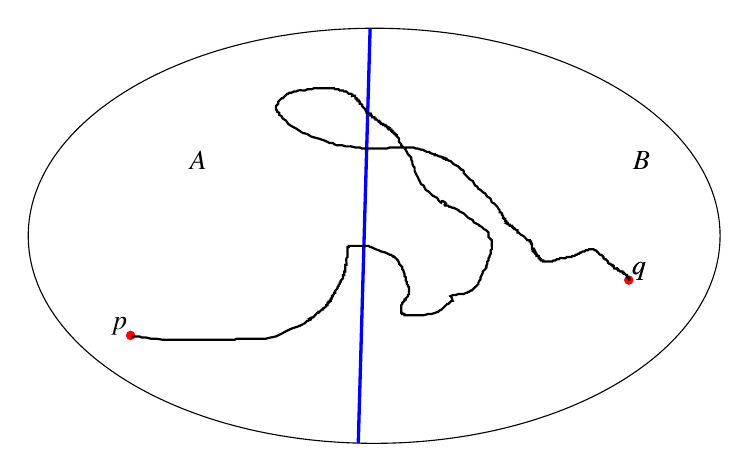
\begin{tikzpicture}[y=0.80pt,x=0.80pt,yscale=-1,scale=0.5, inner sep=0pt, outer sep=0pt]
\draw [clip] (417,520) circle (250pt and 150pt);
\draw (194,610) node [anchor=south east] {$p$};
\filldraw [red] (197,610) circle (3pt);
\draw (650,560) node [anchor=south west] {$q$};
\filldraw [red] (647,560) circle (3pt);
\draw (650,560) node [anchor=south west] {$q$};
\draw [-, very thick,blue] (420,100) -- (380,1500);
\draw (250,460) node [anchor=south west] {$A$};
\draw (650,460) node [anchor=south west] {$B$};


  \path[draw=black,line join=miter,line cap=butt,line width=0.800pt]
    (197.9899,610.9255) .. controls (200.2859,611.5418) and (202.7497,610.4633) ..
    (205.0610,610.9255) .. controls (205.7993,611.0732) and (206.3386,611.8119) ..
    (207.0813,611.9357) .. controls (208.4098,612.1571) and (209.7854,611.7686) ..
    (211.1219,611.9357) .. controls (212.4995,612.1079) and (213.7827,612.7925) ..
    (215.1625,612.9458) .. controls (216.8358,613.1318) and (218.5366,612.7934) ..
    (220.2132,612.9458) .. controls (222.2530,613.1313) and (224.2331,613.7859) ..
    (226.2742,613.9560) .. controls (228.2875,614.1238) and (230.3148,613.9560) ..
    (232.3351,613.9560) .. controls (235.0288,613.9560) and (237.7226,613.9560) ..
    (240.4163,613.9560) .. controls (249.8444,613.9560) and (259.2725,613.9560) ..
    (268.7006,613.9560) .. controls (273.4146,613.9560) and (278.1287,613.9560) ..
    (282.8427,613.9560) .. controls (284.8630,613.9560) and (286.8833,613.9560) ..
    (288.9036,613.9560) .. controls (289.5771,613.9560) and (290.2706,614.1193) ..
    (290.9239,613.9560) .. controls (291.6544,613.7734) and (292.2300,613.1839) ..
    (292.9442,612.9458) .. controls (293.5831,612.7329) and (294.2911,612.9458) ..
    (294.9645,612.9458) .. controls (297.3216,612.9458) and (299.6786,612.9458) ..
    (302.0356,612.9458) .. controls (305.4028,612.9458) and (308.7700,612.9458) ..
    (312.1371,612.9458) .. controls (313.4840,612.9458) and (314.8309,612.9458) ..
    (316.1778,612.9458) .. controls (317.1879,612.9458) and (318.2082,613.0887) ..
    (319.2082,612.9458) .. controls (320.5826,612.7495) and (321.8936,612.2368) ..
    (323.2488,611.9357) .. controls (324.9249,611.5632) and (326.6708,611.4685) ..
    (328.2996,610.9255) .. controls (329.7282,610.4493) and (330.9933,609.5787) ..
    (332.3402,608.9052) .. controls (335.7074,607.2216) and (338.9667,605.3024) ..
    (342.4417,603.8545) .. controls (344.4075,603.0354) and (346.5086,602.5819) ..
    (348.5026,601.8342) .. controls (349.6507,601.4036) and (353.5612,599.4719) ..
    (354.5635,598.8037) .. controls (355.3560,598.2754) and (355.7320,597.2093) ..
    (356.5839,596.7834) .. controls (356.8850,596.6328) and (357.2573,596.7834) ..
    (357.5940,596.7834) .. controls (357.9307,596.4467) and (358.1782,595.9862) ..
    (358.6042,595.7732) .. controls (358.9053,595.6227) and (359.3762,596.0113) ..
    (359.6143,595.7732) .. controls (361.7044,593.6832) and (356.4205,595.8549) ..
    (360.6245,593.7529) .. controls (360.9256,593.6023) and (361.3334,593.9035) ..
    (361.6346,593.7529) .. controls (362.6286,593.2559) and (364.6812,590.2093) ..
    (365.6752,589.7123) .. controls (365.9764,589.5617) and (366.4473,589.9504) ..
    (366.6854,589.7123) .. controls (366.9235,589.4742) and (366.4473,588.9403) ..
    (366.6854,588.7022) .. controls (366.9235,588.4641) and (367.3944,588.8528) ..
    (367.6955,588.7022) .. controls (368.5474,588.2763) and (368.8640,587.1078) ..
    (369.7158,586.6819) .. controls (370.0170,586.5313) and (370.4879,586.9200) ..
    (370.7260,586.6819) .. controls (370.9641,586.4438) and (370.4879,585.9098) ..
    (370.7260,585.6717) .. controls (371.9563,584.4414) and (372.9829,585.1985) ..
    (373.7564,583.6514) .. controls (373.9070,583.3502) and (373.5184,582.8793) ..
    (373.7564,582.6413) .. controls (373.9945,582.4032) and (374.5285,582.8793) ..
    (374.7666,582.6413) .. controls (375.2428,582.1651) and (374.2904,581.0971) ..
    (374.7666,580.6209) .. controls (375.0047,580.3829) and (375.5387,580.8590) ..
    (375.7768,580.6209) .. controls (376.0148,580.3829) and (375.5387,579.8489) ..
    (375.7768,579.6108) .. controls (376.0148,579.3727) and (376.5488,579.8489) ..
    (376.7869,579.6108) .. controls (377.0250,579.3727) and (376.5488,578.8387) ..
    (376.7869,578.6006) .. controls (377.0250,578.3625) and (377.5590,578.8387) ..
    (377.7971,578.6006) .. controls (378.2732,578.1245) and (377.3209,577.0565) ..
    (377.7971,576.5803) .. controls (378.0352,576.3422) and (378.5691,576.8184) ..
    (378.8072,576.5803) .. controls (379.2834,576.1041) and (378.3310,575.0362) ..
    (378.8072,574.5600) .. controls (379.0453,574.3219) and (379.5793,574.7981) ..
    (379.8174,574.5600) .. controls (380.0555,574.3219) and (379.6668,573.8511) ..
    (379.8174,573.5499) .. controls (380.0303,573.1240) and (380.6146,572.9656) ..
    (380.8275,572.5397) .. controls (380.9781,572.2386) and (380.5894,571.7677) ..
    (380.8275,571.5296) .. controls (381.0656,571.2915) and (381.5996,571.7677) ..
    (381.8377,571.5296) .. controls (382.3139,571.0534) and (381.5365,570.1116) ..
    (381.8377,569.5093) .. controls (382.2636,568.6574) and (383.4321,568.3408) ..
    (383.8580,567.4890) .. controls (384.0086,567.1878) and (383.7074,566.7800) ..
    (383.8580,566.4788) .. controls (384.0709,566.0529) and (384.6552,565.8946) ..
    (384.8681,565.4687) .. controls (385.0187,565.1675) and (384.7175,564.7597) ..
    (384.8681,564.4585) .. controls (385.0811,564.0326) and (385.6653,563.8743) ..
    (385.8783,563.4484) .. controls (386.0289,563.1472) and (385.7277,562.7394) ..
    (385.8783,562.4382) .. controls (386.0912,562.0123) and (386.6755,561.8540) ..
    (386.8884,561.4281) .. controls (387.0390,561.1269) and (386.7378,560.7191) ..
    (386.8884,560.4179) .. controls (387.3143,559.5661) and (388.4828,559.2494) ..
    (388.9087,558.3976) .. controls (389.1090,557.9971) and (388.7022,555.5736) ..
    (388.9087,555.3671) .. controls (389.1468,555.1290) and (389.6808,555.6052) ..
    (389.9189,555.3671) .. controls (390.4240,554.8621) and (389.4138,552.8418) ..
    (389.9189,552.3367) .. controls (390.1570,552.0986) and (390.6909,552.5748) ..
    (390.9290,552.3367) .. controls (391.1671,552.0986) and (390.9290,551.6632) ..
    (390.9290,551.3265) .. controls (390.9290,550.8502) and (390.8832,546.3215) ..
    (390.9290,546.2758) .. controls (391.1671,546.0377) and (391.7011,546.5139) ..
    (391.9392,546.2758) .. controls (392.1773,546.0377) and (391.9392,545.6023) ..
    (391.9392,545.2656) .. controls (391.9392,544.5630) and (391.7565,540.5802) ..
    (391.9392,540.2148) .. controls (393.1874,537.7184) and (392.9493,540.5635) ..
    (392.9493,538.1945) .. controls (392.9493,535.8375) and (392.9493,533.4805) ..
    (392.9493,531.1235) .. controls (392.9493,530.7868) and (392.7112,530.3514) ..
    (392.9493,530.1133) .. controls (393.1874,529.8752) and (393.7214,530.3514) ..
    (393.9595,530.1133) .. controls (394.1976,529.8752) and (393.6583,529.2538) ..
    (393.9595,529.1032) .. controls (394.8630,528.6514) and (395.9798,529.1032) ..
    (396.9900,529.1032) .. controls (399.6837,529.1032) and (402.3774,529.1032) ..
    (405.0712,529.1032) .. controls (406.7548,529.1032) and (408.4384,529.1032) ..
    (410.1219,529.1032) .. controls (410.4587,529.1032) and (410.7954,529.1032) ..
    (411.1321,529.1032) .. controls (411.4688,529.1032) and (411.8411,528.9526) ..
    (412.1422,529.1032) .. controls (412.5682,529.3161) and (412.7265,529.9004) ..
    (413.1524,530.1133) .. controls (413.4536,530.2639) and (413.8431,530.0068) ..
    (414.1625,530.1133) .. controls (415.5911,530.5895) and (416.8050,531.5744) ..
    (418.2032,532.1336) .. controls (419.1918,532.5291) and (420.2450,532.7483) ..
    (421.2336,533.1438) .. controls (421.9327,533.4234) and (422.5396,533.9158) ..
    (423.2539,534.1539) .. controls (424.5710,534.5930) and (425.9775,534.7251) ..
    (427.2945,535.1641) .. controls (428.7231,535.6403) and (429.9066,536.7082) ..
    (431.3351,537.1844) .. controls (431.6546,537.2909) and (432.0441,537.0338) ..
    (432.3453,537.1844) .. controls (432.7712,537.3973) and (432.9295,537.9816) ..
    (433.3554,538.1945) .. controls (433.6566,538.3451) and (434.1275,537.9564) ..
    (434.3656,538.1945) .. controls (434.6037,538.4326) and (434.1275,538.9666) ..
    (434.3656,539.2047) .. controls (434.6037,539.4428) and (435.0746,539.0541) ..
    (435.3758,539.2047) .. controls (435.7937,539.4137) and (438.1208,541.8070) ..
    (438.4062,542.2352) .. controls (438.7429,542.9086) and (439.0796,543.5820) ..
    (439.4164,544.2555) .. controls (439.4164,544.5922) and (439.2658,544.9644) ..
    (439.4164,545.2656) .. controls (439.8022,546.0373) and (442.2188,547.6120) ..
    (442.4468,548.2961) .. controls (442.6598,548.9349) and (442.2339,549.6775) ..
    (442.4468,550.3164) .. controls (442.5974,550.7681) and (443.2440,550.9006) ..
    (443.4570,551.3265) .. controls (443.6076,551.6277) and (443.3505,552.0172) ..
    (443.4570,552.3367) .. controls (443.6951,553.0510) and (444.2845,553.6265) ..
    (444.4671,554.3570) .. controls (444.6305,555.0103) and (444.2542,555.7384) ..
    (444.4671,556.3773) .. controls (444.6177,556.8290) and (445.2643,556.9615) ..
    (445.4773,557.3874) .. controls (445.6279,557.6886) and (445.4773,558.0609) ..
    (445.4773,558.3976) .. controls (445.4773,559.0710) and (445.2643,559.7790) ..
    (445.4773,560.4179) .. controls (445.6279,560.8697) and (446.3368,560.9763) ..
    (446.4874,561.4281) .. controls (446.7004,562.0669) and (446.2745,562.8095) ..
    (446.4874,563.4484) .. controls (446.6380,563.9001) and (447.2846,564.0326) ..
    (447.4976,564.4585) .. controls (447.6482,564.7597) and (447.3470,565.1675) ..
    (447.4976,565.4687) .. controls (447.7105,565.8946) and (448.2948,566.0529) ..
    (448.5077,566.4788) .. controls (448.5767,566.6168) and (448.5767,572.4018) ..
    (448.5077,572.5397) .. controls (448.2948,572.9656) and (447.7105,573.1240) ..
    (447.4976,573.5499) .. controls (447.3470,573.8511) and (447.6482,574.2589) ..
    (447.4976,574.5600) .. controls (447.0717,575.4119) and (445.9032,575.7285) ..
    (445.4773,576.5803) .. controls (445.3267,576.8815) and (445.7154,577.3524) ..
    (445.4773,577.5905) .. controls (445.2392,577.8286) and (444.7052,577.3524) ..
    (444.4671,577.5905) .. controls (444.2290,577.8286) and (444.6177,578.2995) ..
    (444.4671,578.6006) .. controls (444.0412,579.4525) and (442.8727,579.7691) ..
    (442.4468,580.6209) .. controls (442.2962,580.9221) and (442.5974,581.3299) ..
    (442.4468,581.6311) .. controls (442.2339,582.0570) and (441.6496,582.2153) ..
    (441.4367,582.6413) .. controls (441.3039,582.9069) and (441.4367,586.1536) ..
    (441.4367,586.6819) .. controls (441.4367,586.9269) and (441.4042,589.6798) ..
    (441.4367,589.7123) .. controls (441.6748,589.9504) and (442.2087,589.4742) ..
    (442.4468,589.7123) .. controls (442.6849,589.9504) and (442.2087,590.4844) ..
    (442.4468,590.7225) .. controls (442.9230,591.1987) and (443.9909,590.2463) ..
    (444.4671,590.7225) .. controls (444.7052,590.9606) and (444.2290,591.4945) ..
    (444.4671,591.7326) .. controls (444.7052,591.9707) and (445.1406,591.7326) ..
    (445.4773,591.7326) .. controls (447.8343,591.7326) and (450.1913,591.7326) ..
    (452.5483,591.7326) .. controls (454.5687,591.7326) and (456.5890,591.7326) ..
    (458.6093,591.7326) .. controls (459.6194,591.7326) and (460.6397,591.8755) ..
    (461.6397,591.7326) .. controls (463.0141,591.5363) and (464.3060,590.9188) ..
    (465.6803,590.7225) .. controls (466.6803,590.5796) and (467.7144,590.8885) ..
    (468.7108,590.7225) .. controls (469.7611,590.5474) and (470.7311,590.0490) ..
    (471.7412,589.7123) .. controls (472.7514,589.3756) and (473.8193,589.1784) ..
    (474.7717,588.7022) .. controls (475.1976,588.4892) and (475.3856,587.9562) ..
    (475.7819,587.6920) .. controls (476.4083,587.2744) and (477.1757,587.0995) ..
    (477.8022,586.6819) .. controls (478.6738,586.1008) and (480.0436,584.4404) ..
    (480.8326,583.6514) .. controls (481.1693,583.3147) and (481.5061,582.9780) ..
    (481.8428,582.6413) .. controls (482.1795,582.3045) and (482.4270,581.8441) ..
    (482.8529,581.6311) .. controls (483.1541,581.4805) and (483.5619,581.7817) ..
    (483.8631,581.6311) .. controls (485.0753,581.0250) and (485.6813,579.2067) ..
    (486.8935,578.6006) .. controls (487.1947,578.4501) and (487.9037,578.9374) ..
    (487.9037,578.6006) .. controls (487.9037,577.5358) and (487.3697,576.5226) ..
    (486.8935,575.5702) .. controls (486.6806,575.1443) and (485.6704,574.9860) ..
    (485.8834,574.5600) .. controls (486.8508,572.6252) and (489.5250,574.0196) ..
    (490.9341,573.5499) .. controls (491.6484,573.3118) and (492.2161,572.6874) ..
    (492.9544,572.5397) .. controls (494.6053,572.2095) and (496.3719,572.9481) ..
    (498.0052,572.5397) .. controls (498.7357,572.3571) and (499.3112,571.7677) ..
    (500.0255,571.5296) .. controls (500.3450,571.4231) and (500.7345,571.6802) ..
    (501.0357,571.5296) .. controls (501.4616,571.3166) and (501.6199,570.7324) ..
    (502.0458,570.5194) .. controls (502.3470,570.3688) and (502.7548,570.6700) ..
    (503.0560,570.5194) .. controls (503.4819,570.3065) and (503.6402,569.7222) ..
    (504.0661,569.5093) .. controls (504.3673,569.3587) and (504.7751,569.6599) ..
    (505.0763,569.5093) .. controls (505.5022,569.2963) and (505.7497,568.8358) ..
    (506.0864,568.4991) .. controls (506.4231,568.1624) and (506.7599,567.8257) ..
    (507.0966,567.4890) .. controls (507.6907,566.8949) and (510.9033,563.9161) ..
    (511.1372,563.4484) .. controls (511.2878,563.1472) and (511.1372,562.7749) ..
    (511.1372,562.4382) .. controls (511.4739,561.7648) and (511.7297,561.0444) ..
    (512.1473,560.4179) .. controls (512.4115,560.0217) and (512.9445,559.8337) ..
    (513.1575,559.4077) .. controls (513.4587,558.8054) and (512.9445,558.0263) ..
    (513.1575,557.3874) .. controls (513.6337,555.9589) and (514.7016,554.7754) ..
    (515.1778,553.3468) .. controls (515.2843,553.0274) and (514.9910,552.6168) ..
    (515.1778,552.3367) .. controls (515.7061,551.5442) and (516.6267,551.0783) ..
    (517.1981,550.3164) .. controls (520.2600,546.2339) and (517.3581,549.8365) ..
    (518.2083,547.2859) .. controls (518.4464,546.5716) and (519.0358,545.9961) ..
    (519.2184,545.2656) .. controls (519.3817,544.6123) and (519.0055,543.8842) ..
    (519.2184,543.2453) .. controls (519.3690,542.7936) and (520.0780,542.6869) ..
    (520.2286,542.2352) .. controls (520.4415,541.5963) and (520.0156,540.8537) ..
    (520.2286,540.2148) .. controls (520.3792,539.7631) and (521.0258,539.6306) ..
    (521.2387,539.2047) .. controls (521.3893,538.9035) and (521.1322,538.5140) ..
    (521.2387,538.1945) .. controls (521.4768,537.4803) and (522.0108,536.8885) ..
    (522.2489,536.1742) .. controls (522.5683,535.2159) and (521.9294,534.1021) ..
    (522.2489,533.1438) .. controls (522.3995,532.6920) and (523.1084,532.5854) ..
    (523.2590,532.1336) .. controls (523.4520,531.5548) and (523.2590,528.0312) ..
    (523.2590,527.0829) .. controls (523.2590,526.0727) and (523.7108,524.9559) ..
    (523.2590,524.0524) .. controls (522.8331,523.2006) and (521.9122,522.7055) ..
    (521.2387,522.0321) .. controls (520.9020,521.6954) and (520.3792,521.4737) ..
    (520.2286,521.0219) .. controls (519.9600,520.2164) and (520.4971,517.7869) ..
    (520.2286,516.9813) .. controls (520.0780,516.5296) and (519.5551,516.3079) ..
    (519.2184,515.9712) .. controls (518.8817,515.6345) and (518.6045,515.2252) ..
    (518.2083,514.9610) .. controls (517.5818,514.5434) and (516.8144,514.3685) ..
    (516.1880,513.9509) .. controls (515.3955,513.4226) and (514.9601,512.4589) ..
    (514.1677,511.9306) .. controls (506.8435,508.2685) and (515.7648,512.9954) ..
    (511.1372,509.9103) .. controls (510.9490,509.7848) and (507.1613,507.9547) ..
    (507.0966,507.8900) .. controls (506.5642,507.3576) and (506.6188,506.4021) ..
    (506.0864,505.8697) .. controls (505.0216,504.8049) and (503.2505,504.7529) ..
    (502.0458,503.8494) .. controls (500.8011,502.9158) and (499.2912,500.6661) ..
    (498.0052,499.8087) .. controls (496.7523,498.9735) and (495.2175,498.6237) ..
    (493.9646,497.7884) .. controls (489.3370,494.7033) and (498.2583,499.4302) ..
    (490.9341,495.7681) .. controls (490.2607,495.4314) and (489.5873,495.0947) ..
    (488.9138,494.7580) .. controls (488.5771,494.7580) and (488.2231,494.8645) ..
    (487.9037,494.7580) .. controls (487.1894,494.5199) and (486.5977,493.9859) ..
    (485.8834,493.7478) .. controls (485.5639,493.6414) and (485.1744,493.8984) ..
    (484.8732,493.7478) .. controls (484.4473,493.5349) and (484.3148,492.8883) ..
    (483.8631,492.7377) .. controls (483.8581,492.7357) and (480.8336,492.7386) ..
    (480.8326,492.7377) .. controls (479.3174,491.2224) and (483.8631,491.7275) ..
    (480.8326,489.7072) .. controls (475.3665,486.0632) and (479.9599,492.8751) ..
    (475.7819,488.6971) .. controls (473.3284,486.2436) and (476.0822,487.2137) ..
    (473.7615,485.6666) .. controls (472.5086,484.8313) and (470.9739,484.4816) ..
    (469.7209,483.6463) .. controls (468.2345,482.6554) and (467.1667,480.5966) ..
    (465.6803,479.6057) .. controls (465.0539,479.1880) and (464.1924,479.1279) ..
    (463.6600,478.5955) .. controls (462.5952,477.5307) and (462.7045,475.6197) ..
    (461.6397,474.5549) .. controls (461.1073,474.0225) and (460.1518,474.0772) ..
    (459.6194,473.5448) .. controls (459.1554,473.0807) and (457.0176,468.3411) ..
    (456.5890,467.4839) .. controls (456.1189,466.5438) and (453.7084,462.1724) ..
    (453.5585,461.4229) .. controls (453.3604,460.4324) and (453.8035,459.3725) ..
    (453.5585,458.3925) .. controls (453.4430,457.9305) and (452.8125,457.7786) ..
    (452.5483,457.3823) .. controls (452.1307,456.7559) and (451.7208,456.0925) ..
    (451.5382,455.3620) .. controls (451.3749,454.7087) and (451.5382,454.0152) ..
    (451.5382,453.3417) .. controls (451.2015,452.6683) and (450.7107,452.0519) ..
    (450.5280,451.3214) .. controls (450.3647,450.6681) and (450.8292,449.9035) ..
    (450.5280,449.3011) .. controls (449.5179,447.2808) and (448.5077,447.7859) ..
    (447.4976,446.2707) .. controls (446.6623,445.0177) and (446.3126,443.4830) ..
    (445.4773,442.2301) .. controls (444.8962,441.3584) and (443.2358,439.9886) ..
    (442.4468,439.1996) .. controls (442.1101,438.8629) and (441.6496,438.6154) ..
    (441.4367,438.1894) .. controls (441.2861,437.8883) and (441.5873,437.4805) ..
    (441.4367,437.1793) .. controls (440.5374,435.3807) and (440.3157,436.9576) ..
    (439.4164,435.1590) .. controls (439.2658,434.8578) and (439.4164,434.4855) ..
    (439.4164,434.1488) .. controls (439.4164,433.4754) and (439.6293,432.7674) ..
    (439.4164,432.1285) .. controls (439.1152,431.2250) and (437.8220,430.9601) ..
    (437.3961,430.1082) .. controls (437.2455,429.8071) and (437.6342,429.3362) ..
    (437.3961,429.0981) .. controls (437.1580,428.8600) and (436.6240,429.3362) ..
    (436.3859,429.0981) .. controls (436.1478,428.8600) and (436.6240,428.3260) ..
    (436.3859,428.0879) .. controls (436.1478,427.8498) and (435.6138,428.3260) ..
    (435.3758,428.0879) .. controls (435.1377,427.8498) and (435.6138,427.3159) ..
    (435.3758,427.0778) .. controls (435.1377,426.8397) and (434.6037,427.3159) ..
    (434.3656,427.0778) .. controls (434.1275,426.8397) and (434.6037,426.3057) ..
    (434.3656,426.0676) .. controls (434.1275,425.8295) and (433.5935,426.3057) ..
    (433.3554,426.0676) .. controls (433.1174,425.8295) and (433.5935,425.2956) ..
    (433.3554,425.0575) .. controls (433.1174,424.8194) and (432.5834,425.2956) ..
    (432.3453,425.0575) .. controls (432.1072,424.8194) and (432.5834,424.2854) ..
    (432.3453,424.0473) .. controls (431.8691,423.5711) and (430.8012,424.5235) ..
    (430.3250,424.0473) .. controls (430.0869,423.8092) and (430.5631,423.2752) ..
    (430.3250,423.0372) .. controls (430.0869,422.7991) and (429.5529,423.2752) ..
    (429.3148,423.0372) .. controls (427.2248,420.9471) and (432.5087,423.1189) ..
    (428.3047,421.0168) .. controls (428.0035,420.8663) and (427.5326,421.2549) ..
    (427.2945,421.0168) .. controls (427.0564,420.7788) and (427.5326,420.2448) ..
    (427.2945,420.0067) .. controls (426.8183,419.5305) and (425.7504,420.4829) ..
    (425.2742,420.0067) .. controls (425.0361,419.7686) and (425.5123,419.2346) ..
    (425.2742,418.9965) .. controls (424.7980,418.5204) and (423.7301,419.4727) ..
    (423.2539,418.9965) .. controls (423.0158,418.7584) and (423.4920,418.2245) ..
    (423.2539,417.9864) .. controls (423.0158,417.7483) and (422.4819,418.2245) ..
    (422.2438,417.9864) .. controls (422.2438,415.2926) and (422.5805,418.3231) ..
    (421.2336,416.9762) .. controls (420.9955,416.7381) and (421.4717,416.2042) ..
    (421.2336,415.9661) .. controls (420.9955,415.7280) and (420.5246,416.1167) ..
    (420.2235,415.9661) .. controls (419.7975,415.7531) and (419.6392,415.1689) ..
    (419.2133,414.9559) .. controls (418.9121,414.8053) and (418.4413,415.1940) ..
    (418.2032,414.9559) .. controls (417.9651,414.7178) and (418.4413,414.1839) ..
    (418.2032,413.9458) .. controls (417.9651,413.7077) and (417.4311,414.1839) ..
    (417.1930,413.9458) .. controls (416.9549,413.7077) and (417.4942,413.0862) ..
    (417.1930,412.9356) .. controls (416.5907,412.6345) and (415.7750,413.2368) ..
    (415.1727,412.9356) .. controls (414.8715,412.7850) and (415.3233,412.2266) ..
    (415.1727,411.9255) .. controls (413.0707,407.7215) and (415.2424,413.0054) ..
    (413.1524,410.9153) .. controls (412.9143,410.6772) and (413.3905,410.1433) ..
    (413.1524,409.9052) .. controls (412.6200,409.3728) and (411.8464,409.1331) ..
    (411.1321,408.8950) .. controls (410.8127,408.7885) and (410.3600,409.1331) ..
    (410.1219,408.8950) .. controls (409.8838,408.6569) and (410.2725,408.1860) ..
    (410.1219,407.8849) .. controls (409.9090,407.4589) and (409.3247,407.3006) ..
    (409.1118,406.8747) .. controls (408.9612,406.5735) and (409.2624,406.1657) ..
    (409.1118,405.8646) .. controls (408.5057,404.6524) and (406.6874,404.0463) ..
    (406.0813,402.8341) .. controls (405.3846,401.4407) and (407.3047,401.9305) ..
    (405.0712,400.8138) .. controls (404.7700,400.6632) and (404.2991,401.0519) ..
    (404.0610,400.8138) .. controls (403.5848,400.3376) and (404.5372,399.2697) ..
    (404.0610,398.7935) .. controls (403.8229,398.5554) and (403.2890,399.0316) ..
    (403.0509,398.7935) .. controls (403.0509,396.0998) and (403.3876,399.1302) ..
    (402.0407,397.7833) .. controls (401.8026,397.5452) and (402.2788,397.0113) ..
    (402.0407,396.7732) .. controls (401.8026,396.5351) and (401.2687,397.0113) ..
    (401.0306,396.7732) .. controls (400.7925,396.5351) and (401.0306,396.0998) ..
    (401.0306,395.7630) .. controls (400.6938,395.7630) and (400.2585,396.0011) ..
    (400.0204,395.7630) .. controls (399.7823,395.5249) and (400.2585,394.9910) ..
    (400.0204,394.7529) .. controls (399.9577,391.9086) and (397.7429,394.4957) ..
    (396.9900,393.7427) .. controls (395.6431,392.3959) and (399.1328,392.7734) ..
    (395.9798,391.7224) .. controls (395.3409,391.5095) and (394.5984,391.9354) ..
    (393.9595,391.7224) .. controls (393.0560,391.4213) and (392.7910,390.1280) ..
    (391.9392,389.7021) .. controls (390.8651,389.1651) and (390.9930,390.2392) ..
    (389.9189,389.7021) .. controls (389.4930,389.4892) and (389.3347,388.9049) ..
    (388.9087,388.6920) .. controls (388.1006,388.2879) and (386.6864,389.0960) ..
    (385.8783,388.6920) .. controls (385.4524,388.4790) and (385.2940,387.8948) ..
    (384.8681,387.6818) .. controls (384.0600,387.2778) and (382.6458,388.0859) ..
    (381.8377,387.6818) .. controls (381.4117,387.4689) and (381.2534,386.8846) ..
    (380.8275,386.6717) .. controls (380.5263,386.5211) and (380.1541,386.6717) ..
    (379.8174,386.6717) .. controls (379.4806,386.6717) and (379.1439,386.6717) ..
    (378.8072,386.6717) .. controls (377.1236,386.6717) and (375.4400,386.6717) ..
    (373.7564,386.6717) .. controls (371.0627,386.6717) and (368.3690,386.6717) ..
    (365.6752,386.6717) .. controls (365.0114,386.6717) and (363.2147,386.4817) ..
    (362.6448,386.6717) .. controls (361.9305,386.9098) and (361.3387,387.4437) ..
    (360.6245,387.6818) .. controls (359.5511,388.0396) and (357.6572,387.3240) ..
    (356.5838,387.6818) .. controls (355.8696,387.9199) and (355.2778,388.4539) ..
    (354.5635,388.6920) .. controls (354.2441,388.7984) and (353.8901,388.6920) ..
    (353.5534,388.6920) .. controls (352.9890,388.6920) and (349.0987,388.4933) ..
    (348.5026,388.6920) .. controls (347.7883,388.9301) and (347.1966,389.4640) ..
    (346.4823,389.7021) .. controls (345.8434,389.9151) and (345.1009,389.4892) ..
    (344.4620,389.7021) .. controls (343.7477,389.9402) and (343.1560,390.4742) ..
    (342.4417,390.7123) .. controls (341.8028,390.9252) and (341.0237,390.4111) ..
    (340.4214,390.7123) .. controls (339.9955,390.9252) and (339.8372,391.5095) ..
    (339.4113,391.7224) .. controls (339.1101,391.8730) and (338.7023,391.5718) ..
    (338.4011,391.7224) .. controls (337.9752,391.9354) and (337.7277,392.3959) ..
    (337.3909,392.7326) .. controls (337.0542,393.0693) and (336.7175,393.4060) ..
    (336.3808,393.7427) .. controls (336.0441,394.0794) and (335.7074,394.4162) ..
    (335.3706,394.7529) .. controls (335.0339,395.0896) and (334.7864,395.5501) ..
    (334.3605,395.7630) .. controls (334.0593,395.9136) and (333.6305,395.5763) ..
    (333.3503,395.7630) .. controls (332.5579,396.2913) and (332.0035,397.1099) ..
    (331.3300,397.7833) .. controls (330.9933,398.1201) and (330.5328,398.3676) ..
    (330.3199,398.7935) .. controls (330.0187,399.3958) and (330.6210,400.2115) ..
    (330.3199,400.8138) .. controls (329.8940,401.6656) and (328.7255,401.9823) ..
    (328.2996,402.8341) .. controls (328.2732,402.8869) and (328.2732,405.8117) ..
    (328.2996,405.8646) .. controls (328.5125,406.2905) and (329.0968,406.4488) ..
    (329.3097,406.8747) .. controls (329.4603,407.1759) and (329.0716,407.6468) ..
    (329.3097,407.8849) .. controls (329.8421,408.4173) and (330.9124,408.2685) ..
    (331.3300,408.8950) .. controls (331.7036,409.4553) and (330.9565,410.3550) ..
    (331.3300,410.9153) .. controls (331.7477,411.5418) and (332.8179,411.3931) ..
    (333.3503,411.9255) .. controls (333.8827,412.4579) and (333.8281,413.4134) ..
    (334.3605,413.9458) .. controls (335.2190,414.8042) and (336.5325,415.1076) ..
    (337.3909,415.9661) .. controls (338.2494,416.8245) and (338.5528,418.1381) ..
    (339.4113,418.9965) .. controls (341.1584,420.7437) and (344.5016,421.8487) ..
    (346.4823,423.0372) .. controls (348.5644,424.2864) and (350.3715,425.9919) ..
    (352.5432,427.0778) .. controls (353.7850,427.6986) and (355.3078,427.5410) ..
    (356.5838,428.0879) .. controls (357.6997,428.5662) and (358.5284,429.5653) ..
    (359.6143,430.1082) .. controls (361.2290,430.9156) and (365.1750,431.6970) ..
    (366.6854,432.1285) .. controls (367.7092,432.4210) and (368.7057,432.8020) ..
    (369.7158,433.1387) .. controls (370.7260,433.4754) and (371.7676,433.7294) ..
    (372.7463,434.1488) .. controls (374.1304,434.7420) and (375.3390,435.7554) ..
    (376.7869,436.1691) .. controls (377.7582,436.4466) and (378.8374,435.9241) ..
    (379.8174,436.1691) .. controls (380.2793,436.2846) and (380.4313,436.9151) ..
    (380.8275,437.1793) .. controls (381.4540,437.5969) and (382.1335,437.9513) ..
    (382.8478,438.1894) .. controls (383.1672,438.2959) and (383.5213,438.1894) ..
    (383.8580,438.1894) .. controls (385.2048,438.1894) and (386.5652,437.9990) ..
    (387.8986,438.1894) .. controls (388.9527,438.3400) and (389.8849,438.9908) ..
    (390.9290,439.1996) .. controls (392.5799,439.5298) and (394.3131,438.9615) ..
    (395.9798,439.1996) .. controls (397.3542,439.3959) and (398.6510,439.9815) ..
    (400.0204,440.2097) .. controls (401.3490,440.4312) and (402.7544,439.8831) ..
    (404.0610,440.2097) .. controls (404.7915,440.3924) and (405.3509,441.0373) ..
    (406.0813,441.2199) .. controls (406.7347,441.3832) and (407.4282,441.2199) ..
    (408.1016,441.2199) .. controls (410.1219,441.2199) and (412.1422,441.2199) ..
    (414.1625,441.2199) .. controls (417.5297,441.2199) and (420.8969,441.2199) ..
    (424.2641,441.2199) .. controls (425.2742,441.2199) and (426.2844,441.2199) ..
    (427.2945,441.2199) .. controls (427.6312,441.2199) and (427.9780,441.3016) ..
    (428.3047,441.2199) .. controls (429.3377,440.9616) and (430.2910,440.4186) ..
    (431.3351,440.2097) .. controls (431.9955,440.0777) and (432.6820,440.2097) ..
    (433.3554,440.2097) .. controls (435.0390,440.2097) and (436.7226,440.2097) ..
    (438.4062,440.2097) .. controls (441.7734,440.2097) and (445.1406,440.2097) ..
    (448.5077,440.2097) .. controls (449.8546,440.2097) and (451.2276,439.9456) ..
    (452.5483,440.2097) .. controls (453.2866,440.3574) and (453.8382,441.0373) ..
    (454.5687,441.2199) .. controls (455.2220,441.3832) and (455.9286,441.0878) ..
    (456.5890,441.2199) .. controls (457.6331,441.4287) and (458.5864,441.9718) ..
    (459.6194,442.2301) .. controls (459.9461,442.3118) and (460.3101,442.1236) ..
    (460.6296,442.2301) .. controls (462.0581,442.7062) and (463.2093,443.8851) ..
    (464.6702,444.2504) .. controls (465.3235,444.4137) and (466.0516,444.0374) ..
    (466.6905,444.2504) .. controls (467.1422,444.4009) and (467.2747,445.0475) ..
    (467.7006,445.2605) .. controls (468.6530,445.7367) and (469.6981,446.0124) ..
    (470.7311,446.2707) .. controls (471.0578,446.3524) and (471.5031,446.0326) ..
    (471.7412,446.2707) .. controls (471.9793,446.5088) and (471.4401,447.1302) ..
    (471.7412,447.2808) .. controls (472.3436,447.5820) and (473.1082,447.1175) ..
    (473.7615,447.2808) .. controls (474.4920,447.4634) and (475.0676,448.0529) ..
    (475.7819,448.2910) .. controls (476.1013,448.3974) and (476.4726,448.1845) ..
    (476.7920,448.2910) .. controls (484.1090,450.7300) and (475.1994,447.9997) ..
    (479.8225,450.3113) .. controls (480.1236,450.4619) and (480.5314,450.1607) ..
    (480.8326,450.3113) .. controls (481.2585,450.5242) and (481.4169,451.1085) ..
    (481.8428,451.3214) .. controls (482.1439,451.4720) and (482.5335,451.2149) ..
    (482.8529,451.3214) .. controls (483.5672,451.5595) and (484.1589,452.0935) ..
    (484.8732,452.3316) .. controls (485.1927,452.4381) and (485.5822,452.1810) ..
    (485.8834,452.3316) .. controls (486.3093,452.5445) and (486.5568,453.0050) ..
    (486.8935,453.3417) .. controls (487.5670,454.0152) and (488.1519,454.7906) ..
    (488.9138,455.3620) .. controls (490.1185,456.2655) and (491.7015,456.5470) ..
    (492.9544,457.3823) .. controls (493.8740,457.9954) and (495.0896,459.9651) ..
    (495.9849,460.4128) .. controls (496.2861,460.5634) and (496.6939,460.2622) ..
    (496.9951,460.4128) .. controls (499.1628,461.4967) and (497.0416,461.5159) ..
    (498.0052,463.4433) .. controls (498.4311,464.2951) and (499.3521,464.7901) ..
    (500.0255,465.4636) .. controls (500.6725,466.1105) and (503.1208,468.8740) ..
    (504.0661,469.5042) .. controls (504.6926,469.9218) and (505.5540,469.9819) ..
    (506.0864,470.5143) .. controls (507.1512,471.5791) and (507.0419,473.4901) ..
    (508.1067,474.5549) .. controls (508.6391,475.0873) and (509.5946,475.0327) ..
    (510.1270,475.5651) .. controls (510.6594,476.0975) and (510.6048,477.0530) ..
    (511.1372,477.5854) .. controls (511.6696,478.1178) and (512.5310,478.1779) ..
    (513.1575,478.5955) .. controls (513.9499,479.1238) and (514.3854,480.0876) ..
    (515.1778,480.6158) .. controls (515.8043,481.0335) and (516.5716,481.2084) ..
    (517.1981,481.6260) .. controls (519.5188,483.1731) and (516.7650,482.2030) ..
    (519.2184,484.6565) .. controls (520.4488,485.8868) and (521.4753,485.1296) ..
    (522.2489,486.6768) .. controls (522.7251,487.6291) and (522.6201,488.8554) ..
    (523.2590,489.7072) .. controls (523.7108,490.3096) and (524.6770,490.2656) ..
    (525.2793,490.7174) .. controls (526.0412,491.2888) and (526.6262,492.0642) ..
    (527.2996,492.7377) .. controls (527.6364,493.0744) and (528.0456,493.3516) ..
    (528.3098,493.7478) .. controls (528.7274,494.3743) and (528.9023,495.1417) ..
    (529.3199,495.7681) .. controls (529.5841,496.1643) and (530.1795,496.3265) ..
    (530.3301,496.7783) .. controls (530.5431,497.4172) and (530.0289,498.1963) ..
    (530.3301,498.7986) .. controls (530.4807,499.0998) and (531.0391,498.6480) ..
    (531.3402,498.7986) .. controls (533.5737,499.9153) and (531.6537,499.4255) ..
    (532.3504,500.8189) .. controls (532.5634,501.2448) and (533.1476,501.4031) ..
    (533.3605,501.8291) .. controls (533.6617,502.4314) and (532.8844,503.3732) ..
    (533.3605,503.8494) .. controls (533.5986,504.0875) and (534.1326,503.6113) ..
    (534.3707,503.8494) .. controls (534.6088,504.0875) and (534.1326,504.6214) ..
    (534.3707,504.8595) .. controls (534.6088,505.0976) and (535.1428,504.6214) ..
    (535.3809,504.8595) .. controls (535.8570,505.3357) and (534.9047,506.4036) ..
    (535.3809,506.8798) .. controls (535.6189,507.1179) and (536.1529,506.6417) ..
    (536.3910,506.8798) .. controls (536.6291,507.1179) and (536.1529,507.6519) ..
    (536.3910,507.8900) .. controls (536.6291,508.1281) and (537.1631,507.6519) ..
    (537.4012,507.8900) .. controls (539.4912,509.9800) and (534.2073,507.8083) ..
    (538.4113,509.9103) .. controls (538.7125,510.0609) and (539.1834,509.6722) ..
    (539.4215,509.9103) .. controls (539.6596,510.1484) and (539.1834,510.6823) ..
    (539.4215,510.9204) .. controls (539.8976,511.3966) and (540.9656,510.4442) ..
    (541.4418,510.9204) .. controls (541.6799,511.1585) and (541.2037,511.6925) ..
    (541.4418,511.9306) .. controls (541.6799,512.1687) and (542.2138,511.6925) ..
    (542.4519,511.9306) .. controls (542.6900,512.1687) and (542.2138,512.7026) ..
    (542.4519,512.9407) .. controls (542.6900,513.1788) and (543.2240,512.7026) ..
    (543.4621,512.9407) .. controls (543.7002,513.1788) and (543.2240,513.7128) ..
    (543.4621,513.9509) .. controls (543.7002,514.1890) and (544.1711,513.8003) ..
    (544.4722,513.9509) .. controls (544.8981,514.1638) and (545.0565,514.7481) ..
    (545.4824,514.9610) .. controls (545.7835,515.1116) and (546.2544,514.7229) ..
    (546.4925,514.9610) .. controls (546.9687,515.4372) and (546.0163,516.5051) ..
    (546.4925,516.9813) .. controls (546.7306,517.2194) and (547.2015,516.8308) ..
    (547.5027,516.9813) .. controls (548.3545,517.4073) and (548.7306,518.4734) ..
    (549.5230,519.0016) .. controls (550.1495,519.4193) and (550.9168,519.5941) ..
    (551.5433,520.0118) .. controls (552.4149,520.5929) and (553.7847,522.2532) ..
    (554.5737,523.0423) .. controls (554.9105,523.3790) and (555.1580,523.8394) ..
    (555.5839,524.0524) .. controls (556.1862,524.3536) and (557.1280,523.5762) ..
    (557.6042,524.0524) .. controls (557.8423,524.2905) and (557.3661,524.8245) ..
    (557.6042,525.0626) .. controls (557.8423,525.3007) and (558.3763,524.8245) ..
    (558.6144,525.0626) .. controls (559.0905,525.5387) and (558.1382,526.6067) ..
    (558.6144,527.0829) .. controls (558.8524,527.3210) and (559.3864,526.8448) ..
    (559.6245,527.0829) .. controls (559.6570,527.1154) and (559.6245,529.8683) ..
    (559.6245,530.1133) .. controls (559.6245,530.4500) and (559.6245,530.7868) ..
    (559.6245,531.1235) .. controls (559.6245,531.4602) and (559.3864,531.8955) ..
    (559.6245,532.1336) .. controls (559.8626,532.3717) and (560.3966,531.8955) ..
    (560.6347,532.1336) .. controls (560.8728,532.3717) and (560.3966,532.9057) ..
    (560.6347,533.1438) .. controls (562.7247,535.2338) and (560.5530,529.9499) ..
    (562.6550,534.1539) .. controls (562.9561,534.7563) and (562.1788,535.6980) ..
    (562.6550,536.1742) .. controls (562.8931,536.4123) and (563.4270,535.9361) ..
    (563.6651,536.1742) .. controls (564.1413,536.6504) and (563.1889,537.7184) ..
    (563.6651,538.1945) .. controls (563.9032,538.4326) and (564.6753,538.5313) ..
    (564.6753,538.1945) .. controls (564.6753,537.7184) and (563.1889,537.1844) ..
    (563.6651,537.1844) .. controls (564.4180,537.1844) and (565.1530,537.6621) ..
    (565.6854,538.1945) .. controls (566.1616,538.6707) and (565.2092,539.7387) ..
    (565.6854,540.2148) .. controls (565.9235,540.4529) and (566.4575,539.9768) ..
    (566.6956,540.2148) .. controls (566.9337,540.4529) and (566.4575,540.9869) ..
    (566.6956,541.2250) .. controls (566.9337,541.4631) and (567.4676,540.9869) ..
    (567.7057,541.2250) .. controls (567.9438,541.4631) and (567.4676,541.9971) ..
    (567.7057,542.2352) .. controls (568.1819,542.7113) and (569.2498,541.7590) ..
    (569.7260,542.2352) .. controls (569.9641,542.4732) and (569.4879,543.0072) ..
    (569.7260,543.2453) .. controls (569.7585,543.2778) and (572.5115,543.2453) ..
    (572.7565,543.2453) .. controls (573.4591,543.2453) and (577.4419,543.4280) ..
    (577.8073,543.2453) .. controls (578.2332,543.0323) and (578.3915,542.4481) ..
    (578.8174,542.2352) .. controls (579.4197,541.9340) and (580.2354,542.5363) ..
    (580.8377,542.2352) .. controls (581.2636,542.0222) and (581.4219,541.4380) ..
    (581.8479,541.2250) .. controls (582.4502,540.9238) and (583.2658,541.5262) ..
    (583.8682,541.2250) .. controls (584.2941,541.0120) and (584.4524,540.4278) ..
    (584.8783,540.2148) .. controls (585.5156,539.8962) and (589.2918,540.5335) ..
    (589.9291,540.2148) .. controls (590.3550,540.0019) and (590.5133,539.4177) ..
    (590.9392,539.2047) .. controls (591.5741,538.8872) and (594.3449,539.5221) ..
    (594.9798,539.2047) .. controls (595.4058,538.9917) and (595.5641,538.4075) ..
    (595.9900,538.1945) .. controls (597.0679,537.6556) and (596.9324,538.7335) ..
    (598.0103,538.1945) .. controls (598.4362,537.9816) and (598.5945,537.3973) ..
    (599.0205,537.1844) .. controls (599.3216,537.0338) and (599.7294,537.3350) ..
    (600.0306,537.1844) .. controls (600.4565,536.9714) and (600.6148,536.3872) ..
    (601.0408,536.1742) .. controls (601.3419,536.0237) and (601.7497,536.3248) ..
    (602.0509,536.1742) .. controls (602.4768,535.9613) and (602.6351,535.3770) ..
    (603.0611,535.1641) .. controls (603.3622,535.0135) and (603.7700,535.3147) ..
    (604.0712,535.1641) .. controls (604.4971,534.9511) and (604.6555,534.3669) ..
    (605.0814,534.1539) .. controls (605.6837,533.8528) and (606.4993,534.4551) ..
    (607.1017,534.1539) .. controls (607.5276,533.9410) and (607.6859,533.3567) ..
    (608.1118,533.1438) .. controls (608.7142,532.8426) and (609.5298,533.4449) ..
    (610.1321,533.1438) .. controls (610.5581,532.9308) and (610.7164,532.3466) ..
    (611.1423,532.1336) .. controls (611.2284,532.0906) and (615.0968,532.0906) ..
    (615.1829,532.1336) .. controls (615.6088,532.3466) and (615.7671,532.9308) ..
    (616.1930,533.1438) .. controls (616.4942,533.2944) and (616.9020,532.9932) ..
    (617.2032,533.1438) .. controls (618.1972,533.6408) and (620.2498,536.6874) ..
    (621.2438,537.1844) .. controls (624.2165,538.6707) and (619.9139,534.8443) ..
    (623.2641,538.1945) .. controls (623.6008,538.5313) and (624.0613,538.7788) ..
    (624.2743,539.2047) .. controls (624.9709,540.5981) and (623.0509,540.1082) ..
    (625.2844,541.2250) .. controls (625.5856,541.3756) and (625.9934,541.0744) ..
    (626.2946,541.2250) .. controls (626.7205,541.4380) and (626.9680,541.8984) ..
    (627.3047,542.2352) .. controls (627.6414,542.5719) and (628.1019,542.8194) ..
    (628.3149,543.2453) .. controls (629.0116,544.6387) and (627.0915,544.1489) ..
    (629.3250,545.2656) .. controls (629.6262,545.4162) and (629.9985,545.2656) ..
    (630.3352,545.2656) .. controls (630.6719,545.6023) and (630.9194,546.0628) ..
    (631.3453,546.2758) .. controls (631.6465,546.4263) and (632.1174,546.0377) ..
    (632.3555,546.2758) .. controls (632.5936,546.5139) and (632.1174,547.0478) ..
    (632.3555,547.2859) .. controls (632.5936,547.5240) and (633.0289,547.2859) ..
    (633.3656,547.2859) .. controls (633.3656,547.6226) and (633.1275,548.0580) ..
    (633.3656,548.2961) .. controls (633.4283,551.1404) and (635.6432,548.5533) ..
    (636.3961,549.3062) .. controls (636.6342,549.5443) and (636.3961,549.9797) ..
    (636.3961,550.3164) .. controls (636.7328,550.3164) and (637.1682,550.0783) ..
    (637.4063,550.3164) .. controls (637.6443,550.5545) and (637.1682,551.0884) ..
    (637.4063,551.3265) .. controls (637.6443,551.5646) and (638.1152,551.1759) ..
    (638.4164,551.3265) .. controls (638.8423,551.5395) and (639.0898,552.0000) ..
    (639.4266,552.3367) .. controls (640.1000,552.3367) and (640.8445,552.0355) ..
    (641.4469,552.3367) .. controls (641.7480,552.4873) and (641.2088,553.1087) ..
    (641.4469,553.3468) .. controls (641.6850,553.5849) and (642.1203,553.3468) ..
    (642.4570,553.3468) .. controls (642.4570,553.6835) and (642.2189,554.1189) ..
    (642.4570,554.3570) .. controls (642.6951,554.5951) and (643.1660,554.2064) ..
    (643.4672,554.3570) .. controls (643.8931,554.5699) and (644.0514,555.1542) ..
    (644.4773,555.3671) .. controls (644.7785,555.5177) and (645.2494,555.1290) ..
    (645.4875,555.3671) .. controls (645.9637,555.8433) and (645.0113,556.9112) ..
    (645.4875,557.3874) .. controls (645.7256,557.6255) and (646.2595,557.1493) ..
    (646.4976,557.3874) .. controls (646.7357,557.6255) and (646.2595,558.1595) ..
    (646.4976,558.3976) .. controls (646.7357,558.6357) and (647.2697,558.1595) ..
    (647.5078,558.3976) .. controls (647.7459,558.6357) and (647.5078,559.0710) ..
    (647.5078,559.4077) .. controls (647.5078,559.7445) and (647.5078,560.0812) ..
    (647.5078,560.4179);

\end{tikzpicture}



\caption{}
\end{figure}
Dann wäre $[0,1]=c^{-1}(A)\dotcup c^{-1}(B)$ eine Zerlegung in zwei disjunkte, nichtleere offene Mengen.
\end{proof}
Die Umkehrung gilt jedoch im Allgemeinen nicht:
\begin{ex*}
Ein Raum, der zusammenhängend, aber nicht \underline{weg}zusammenhängend ist.
\[
X=\underbrace{\{0\}\times [-1,1]}_{A}\cup\underbrace{\{(x, \sin(x^{-1}))|x>0\}}_{B}
\] 
\begin{figure}[H]
\centering
 \fixme[fig22]
\caption{}
\end{figure}
\end{ex*}
Die Relation $ p\sim q \stackrel{\text{def}}{\iff} $ es gibt einen weg von $ p $ nach $ q $ ist (Übung) offensichtlich eine Äquivalenzrelation, die zugehörigen Äquivalenzklassen heißen \emph{Wegzusammenhangskomponenten} des topologischen Raums.
\begin{st}
\begin{enumerate}[(i)]
\item Stetige Bilder von (weg-)zusammenhängenden Räumen sind (weg-)zusammenhängend.
\item Vereinigungen (weg-)zusammenhängender Räume $ X_i, i\in I, $ mit $ \bigcap X_i\neq \emptyset $ sind (weg-)zusammenhängend.
\item Ein Produkt $ X\times Y $ von (weg-)zusammenhängenden nichtleeren topologischen Räumen $ X,Y $ ist genau dann (weg-)zusammenhängend, wenn die beiden Faktoren es sind. 
\end{enumerate}
\end{st}
\begin{proof}
\item Sei $ f:X\to Y$ stetige Abbildung, zerfällt $f(X)=Y_1\dotcup Y_2$ mit $Y_1, Y_2$ offen disjunkt, so zerfällt auch $ X=f^{-1}(Y_1)\dotcup f^{-1}(Y_2) $. 
\begin{figure}[H]
\centering
 \fixme[fig23]
\caption{}
\end{figure}
Sei $ p,q \in f(X) $. Es gibt $ a,b\in X $ mit $ f(a)=p $, $ f(b)=q $ und einen Weg $ c:[0,1]\to X $ von $ a $ nach $ b $. Dann ist $ f\circ c:[0,1]\to f(X) $ ein Weg von $ p $ nach $ q $.
\item Sei $ X=\bigcup_{i\in I}X_i $. Sei $ X=A\dotcup B $ mit $ A,B $ offen. Sei $ p\in \bigcap_{i\in I}X_i $ und ohne Einschränkung $ p\in A $.  Es gilt $ X_i=(X_i\cap A)\dotcup (X_i\cap B) $, da $ p\in X_i\cap A $ folgt $ X_i\cap B=\emptyset $, denn $ X_i $ ist zusammenhängend. Also folgt $ B=\emptyset $.
Für Wegzusammenhängend:
\begin{figure}[H]
\centering
 \fixme[fig24]
\caption{}
\end{figure}
Es gilt, falls $ c:[0,1]\to X_i $ ein stetiger Weg von $ a\in X_i $ nach $ p $ und $ d:[0,1]\to X_j $ ein stetiger Weg von $ p $ nach $ b\in X_j $ ist, dann ist:
\[
e(t):=\begin{cases}c(2t)\qquad &,t\in[0,\frac 1 2]\\ d(2t-1)\qquad &,t\in[\frac 1 2, 1]\end{cases}
\]
eine stetige Abbildung $ [0,1]\to \bigcup_{i\in I}X_i $. (Übung)
\end{proof}
\begin{df}
 Eine \emph{Zusammenhangskomponente} $e$ eines topologischen Raumes $X$ ist ein maximal zusammenhängender Teilraum.
($A\subset X$ ist \emph{maximal zusammenhängend}, falls es keine zusammenhängende Teilmenge $B\subset X$ gibt mit $A\subset B, A\neq B$)
\end{df}
\begin{st}\label{thm:4.4}
 \begin{enumerate}[(i)]
  \item Ist $A\subset X$ zusammenhängend und $A\subset B\subset \bar A$, so ist auch $B$ zusammenhängend.
  \item Jeder Punkt von $X$ liegt in genau einer Zusammenghangskomponente von $X$, mit anderen Worten. $X$ ist die disjunkte Vereinigung seiner Komponenten.
\item Die Komponenten von $X$ sind abgeschlossene Teilräume.
 \end{enumerate}

\end{st}

\begin{proof}
 \begin{enumerate}[(i)]
  \item Seien $M_1,M_2\subset X$ abgeschlossen mit $B\subset M_1\cup M_2$ und $B\cap M_1\cap M_2=\emptyset$. 
Sei ohne Einschränkung $A\cap M_1\neq \emptyset$. Zu zeigen ist, dass $B\cap M_2=\emptyset$. Da $A$ zusammenhängend ist, gilt $A\subset M_1$, also auch $\bar A \subset M_1$, somit gilt $B\cap M_2=\emptyset$.
\item Die Vereinigung aller zusammenhängenden Teilräume von $X$, die den Punkt $p$ enthalten, ist nach \ref{thm:4.4}(ii)
 zusammenhängend und offenbar die einzige maximal zusammenhängende Teilmenge, die $p$ enthält. (Immer ist $\{p\}$ zusammenhängend)
\item folgt aus (i).
 \end{enumerate}
\end{proof}
\subsection{Abzählbarkeitsaxiome}
\begin{df}
 Sei $(X,O)$ ein topologischer Raum. Eine Teilmenge $\mathcal B\subset O$ heißt \emph{Basis} (der Topologie) von $X$, wenn jedes $U\subset O$ eine Vereinigung von Mengen aus $\mathcal B$ ist.
\end{df}
\begin{exs*}
 \begin{enumerate}
  \item Immer gilt, dass $O$ selbst eine Basis ist.
  \item Im $\R^n$ ist der Menge der offenen $\eps$-Bälle eine Basis der Topologie, aber auch die Menge der achsenparallelen offenen Würfel.
  \item Allgemeiner ist in jedem metrischen Raum die Menge der offenen $\eps$-Bälle eine Basis der Topologie.
  \item Seien $(X_1,O_2)$ und $(X_2,O_2)$ topologische Räume. Dann ist $O_1\times O_2$ eine Basis der Produkttopologie.
\end{enumerate}
\end{exs*}
Kann man beliebige Familien von Teilmengen eines Raumes $X$ vorgeben und fordern, die Topologie solle aus allen Vereinigungen dieser Mengen (und $X$ selbst) bestehen? Nein, man muss auch sicherstellen, dass endliche Schnitte wieder offen sind. Deshalb:
\begin{df}
 Sei $(X,O)$ ein topologischer Raum. Eine Teilmenge $\mathcal S\subset O$ heißt \emph{Subbasis}, wenn die Menge der endlichen Schnitte der Mengen in $\mathcal S$ eine Basis bildet.
\end{df}
\begin{st}\label{thm:4.3}
 Sei $X$ eine Menge und $\mathcal S\subset \Pot(X)$  eine Familie von Teilmengen von $X$. Dann gibt es genau eine Topologie auf $X$, die dieses $S$ als Subbasis hat.
\end{st}
\begin{proof}
Sei $\mathcal B:=\{S_1\cap\dotsb \cap S_n|n\in \N_0, S_1,\dotsc  ,S_n\in \mathcal S\}$ und setze $O:=\{\bigcup_iB_i|B_i\in \mathcal B\} \cup\{\emptyset,X\}$.
 Wir zeigen, dass $O$ eine Topologie auf $X$ ist. Offensichtlich liegen beliebigen Vereinigung von Mengen in $O$ wieder in $O$. 
Sei $U_1=\bigcup_{i\in I_1}B_i, U_2=\bigcup_{i\in I_2}B_i$, mit $B_i\in \mathcal B$. Dann ist:
\[
 U_1\cap U_2=\bigcup\limits_{j\in I_1,k\in I_2}B_j\cap B_k
\]
eine Vereinigung von endlichen Schritten von Mengen in $\mathcal S$, also Element von $O$. (Dies zeigt, dass $O$ eine Topologie auf $X$ ist). 
Jede Topologie auf $X$, die $\mathcal S$ enthält, muss auch $O$ enthalten, andererseits kann eine Topologie mit $\mathcal S$ als Subbasis auch nicht feiner sei als $O$.
\end{proof}
Man sagt auch, $O$ ist die \emph{von $\mathcal S$ erzeugte Topologie}. Dass heißt $O$ entsteht durch Anwenden des früher definierten
Hüllenoperators auf $\mathcal S$, $\mathcal T(\mathcal S)=O$.

Als eine Anwendung wollen wir die Produkttopologie von beliebig (auch unendlich) vielen Räumen erklären.

Seien $(X_\alpha,O_\alpha), \alpha \in A$ topologische Räume und sei
\[
 \bigsqcap X_\alpha=\{f:A\to\bigcup X_\alpha|f(\alpha)\in X_\alpha\}
\]
Wir verwenden als Subbasis die Menge
\[
 \mathcal S:=\{\bigsqcap_\alpha U_\alpha|U_\alpha \in O_\alpha, U_\alpha=X_\alpha \text{ für alle bis auf ein $\alpha \in A$}\}
\]
Die so (nach Satz \ref{thm:4.3}) defnierte Topologie heißt \emph{Produkttopologie} auf $\bigsqcap_\alpha X_\alpha$ (und 
$\mathcal S$ ist eine Subbasis). Dann ist:
\[
 \mathcal B := \{ \bigsqcap_\alpha U_\alpha|U_\alpha\in O_\alpha, U_\alpha=X_\alpha \text{ für alle bis auf endlich viele } \alpha \in A\}
\]
\begin{seg}{Übungsaufgabe}
 Nach Konstruktion ist die Produkttopologie die initiale Topologie bezüglich der kanonischen Projektionen $\pi_\alpha:\bigsqcap_\alpha X_\alpha\to X_\alpha: f\mapsto f(\alpha)$
Die kanonische Projektionenen sind nämlich stetig: Sei $\alpha \in A$. Das Urbild $\pi_\alpha^{-1}$ einer offenen Menge $U\subset X_\alpha$ ist gerade:
\[
 \{\bigsqcap_\beta U_\beta|U_\alpha=U, U_\beta=X_\beta \text{ für } \beta\neq a\}
\]

\end{seg}
\begin{note*}
 \begin{itemize}
  \item $\mathcal S=\{X_1\times X_2\times \dotsb  \times X_{k-1} \times U \times X_{k+1} \times\dotsb \times X_n |U\subset X_k$ offen $, k \in \{1, \dotsc n \} \} $
  \item $\R^3=\{(x_1,x_2,x_3)|x_\alpha\in \R\}$, $\R^3=\{f:\{1,2,3\}\mapsto \R, \alpha\mapsto x_\alpha\}$
 \end{itemize}
\end{note*}
\begin{df}
 Sei $(X,O)$ ein topologischer Raum. Eine Familie $\mathcal U$ von Umgebungen von $p$ heißt \emph{Umgebungsbasis} von $p$, wenn jede Umgebung von $p$ eine Umgebung aus $\mathcal U$ enthält.
\begin{figure}[H]
\centering
 \fixme[fig25]
\caption{}
\end{figure}
\end{df}
\begin{exs*}
 \begin{enumerate}
\item  Im $\R^n$ ist zum Beispiel jede der Mengen $\{B_\eps(p)|\eps>0\}$ , $ \{B_\eps(p)|\eps\in (0,1]\}$, $\{ B_\eps(p)|\eps>0,\eps\in \Q \}$ und $\{B_{n^{-1}}(p)|n\in \N\}$ eine Umgebungsbasis von $p$. Die letzten beiden sind abzählbar.
\item Dies lässt sich auf metrische Räume übertragen: In jedem metrischen Raum $X$ mit $p\in X$ ist $\{B_{n^{-1}}(p)|n\in \N\}$ eine abzählbare Umgebungsbasis von p.
 \end{enumerate}
\end{exs*}
\begin{df}
 \begin{enumerate}[(i)]
  \item Ein topologischer Raum erfüllt das \emph{erste Abzählbarkeitsaxiome}, wenn es um jeden Punkt eine abzählbare Umgebungsbasis gibt. 
\item Ein topologischer Raum erfüllt das \emph{zweite Abzählbarkeitsaxiome}, wenn es eine abzählbare Basis der Topologie gibt.
 \end{enumerate}
\end{df}
\begin{seg}{Zusammenfassung}
Eine Familie von Teilmengen heißt
\begin{itemize}
 \item \emph{Basis}, wenn sich jede offene Teilmenge als Vereinigung von Mengen aus der Basis bilden lässt.
 \item \emph{Subbasis}, wenn endliche Schnitte eine Basis bilden.
 \item \emph{Abzählbarkeitsaxiome}
 \begin{itemize}
\item \emph{Erstes Abzählbarkeitsaxiom}: Um jeden Punkt gibt es ein abzählbare \emph{Umgebungsbasis} (Umgebungsbasis von $p\in X$: eine Familie von Umgebungen $\mathcal U$
, so dass jede Umgebung von p eine Menge aus $\mathcal U$ enthält.)
\item \emph{Zweites Abzählbarkeitsaxiom}: Der Raum besitzt eine abzählbare Basis
\end{itemize}
\end{itemize}
\end{seg}
Der folgende Satz gibt eine Antwort auf die Frage, wie die beiden Abzählbarkeitsaxiome zusammenhängen und eine Antwort auf die Frage, wozu das erste Abzählbarkeitsaxiom nützlich ist.
\begin{st}\label{thm:5.6}
 \begin{enumerate}[(i)]
  \item Das zweite Abzählbarkeitsaxiom impliziert das erste.
  \item Gilt in einem topologischen Raum $X$ das erste Abzählbarkeitsaxiom, dann sind Stetigkeit und Folgenstetigkeit für Abbildungen $f:X\to Y$ äquivalent.
 \end{enumerate}
\end{st}
\begin{proof}
%Gnu Linux : Skript argumentativ abgeändertW
 \begin{enumerate}[(i)]
  \item Sei $\mathcal B$ eine abzählbare Basis der Topologie und $p\in X$ ein beliebiger Punkt. Setze $\mathcal U:=\{U\in \mathcal{B} |p\in U\}$. Sei nun $V$ eine Umgebung von $p$, dann enthält $V$ eine offene Menge $Q$ mit $p\in Q$. Aber $Q$ ist eine Vereinigung von Mengen in $\mathcal B$, also gibt es eine Menge $U\in \mathcal U$ mit  $U \subset V$. Damit ist $ \mathcal U $ eine abzählbare Umgebungsbasis von $p$.
\item \begin{seg}{„$\implies$“} bereits gezeigt in \ref{thm:1.17} \end{seg}

\begin{seg}{„$\Longleftarrow$“} Sei nun $f:X\to Y$ folgenstetig und gelte in $X$ das erste Abzählbarkeitsaxiom. Angenommen, f wäre \emph{nicht} stetig in einem Punkt $x\in X$. Dann gibt es eine Umgebung $U$ von $f(x)$, zu der es \emph{keine} Umgebung $V$ von $x$ gibt mit $f(V)\subset U$. Sei $\mathcal U=\{U_1,U_2,U_3,\dotsc  \}$ eine abzählbare Umgebungsbasis von $x$. Die Mengen $U_1, U_1\cap U_2$, $U_1\cap U_2 \cap U_3,\dotsc  $ Umgebungen von $x$. Nach Annahme gibt es in jeder dieser Mengen $U_1\cap\dotsb \cap U_k$ einen Punkt $x_n$, so dass $f(x_n)$ außerhalb von U liegt. Die Folge $x_n$ konvergiert gegen $x$, die Folge $f(x_n)$ aber \emph{nicht} gegen f(x).
\end{seg}
\end{enumerate}
\end{proof}
\begin{note}
 $f: X\to Y$ heißt \emph{folgenstetig}, falls für alle konvergenten Folgen $x_n\to x$ in $X$ gilt $f(x_n)\to f(x)$ 
\end{note}
\subsection{Kompaktheit}
\begin{df}\label{thm:6.1}
 Eine \emph{offene Überdeckung} eines topologischen Raumes $X$ ist eine Familie $U_i$, $i\in I$, von offenen Teilmengen von $X$ mit der Eigenschaft $\bigcup_{i\in I} U_i=X$.
\end{df}
\begin{df}\label{thm:6.2}
 Ein topologischer Raum $X$ heißt \emph{kompakt}, wenn jede offene Überdeckung von $X$ eine \emph{endliche Teilüberdeckung} besitzt, dass heißt falls folgendes gilt: ist $U_i, i\in I$, eine offene Überdeckung von $X$, so gibt es endlich viele $i_1, \dotsc  ,i_n\in I$, so dass $U_{i_1}\cup \dotsb \cup U_{i_n}=X$ gilt.
\end{df}
\begin{ex*}
 $\R^n$ ist \emph{nicht kompakt}, denn die offene Überdeckung durch $B_k(0),k\in \N$ besitzt k          eine endliche Teilüberdeckung.
\end{ex*}

\begin{note}\label{thm:6.3}
 Manchmal (nicht in dieser Vorlesung) wird zusätzlich noch die Hausdorffeigenschaft verlangt (in diesem Fall heißt die obige Eigenschaft meist "`präkompakt"').
\end{note}
\begin{st}[Heine-Borelscher Überdeckungssatz]\label{thm:1.6.4}
 Eine Teilmenge des $\R^n$ ist kompakt genau dann, wenn sie abgeschlossen und beschränkt ist.
\end{st}
\begin{proof}
 siehe zum Beispiel Forster O., Analysis II.
\end{proof}
\begin{st}\label{thm:1.6.5}
 Jede kompakte Teilmenge eines metrischen Raumes ist beschränkt und abgeschlossen (Umkehrung gilt im Allgemeinen nicht).
\end{st}
\begin{proof}
 \begin{seg}{Beschränktheit:}
  Für einen beliebigen Punkt $x$ bildet $B_k(x)\cap A, k \in \N$, eine offene Überdeckung von $A$, da es eine endliche Teilüberdeckung gibt, ist der Abstand von x durch eine natürliche Zahl beschränkt.
 \end{seg}
\begin{seg}{Abgeschlossenheit:}
 Sei $A\subset X$ kompakt und sei $x\in X\setminus A$. Es gilt:
\[
 U_\eps:=(X\setminus\bar{B_\eps(x)})\cap A, \eps>0 := \{ y\in A|d(x,y) > \eps\}
\]
bilden eine offene Überdeckung von $A$, es gibt eine endliche Teilüberdeckung $U_{\eps_1}\cup\dotsb  \cup U_{\eps_k}$, und es folgt, dass $B_\eps(x)$ mit $\eps:=\min\{\eps_1,\dotsc  ,\eps_k\}$ ganz in $X\setminus A$ liegt.
\begin{figure}[H]
\centering
 \fixme[fig26]
\caption{}
\end{figure}
\end{seg}
\end{proof}
Die Umkehrung gilt in beliebigen metrischen Räumen \emph{nicht}, der Begriff „beschränkt“ lässt sich nicht analog auf metrische Räume übertragen, denn für jede Metrik $d$ auf $X$ ist auch
\[
 d'(x,y):=\frac{d(x,y)}{1+d(x,y)}<1
\]
eine Metrik (die dieselbe Topologie erzeugt) also ist die Unterscheidung zwischen beschränkten und unbeschränkten Mengen hier nicht sehr hilfreich.
\begin{note*}
 Ein metrischer Raum ist kompakt, wenn er \emph{vollständig} und \emph{totalbeschränkt} ist, \emph{totalbeschränkt} bedeutet: zu jedem $\eps>0$ gibt es ein endliches $\eps$-Netz, dass heißt zu jedem $\eps>0$ gibt es endlich viele Punkte $x_1,\dotsc  ,x_k$ mit $\bigcup_{i=1}^kB_\eps(x_i)=X$.
\end{note*}
\begin{st}\label{thm:1.6.6}
 Stetige Bilder kompakter Räume sind kompakt.
\end{st}
\begin{proof}
Sei $f:X\to Y$ stetig und $U_i, i\in I$ eine offene Überdeckung von $Y$. Dann ist $f^{-1}(U_i),i\in I$, eine offene Überdeckung von $X$. Diese besitzt aber eine endliche Teilüberdeckung $f^{-1}(U_{i_1})\cup \dotsb \cup f^{-1}(U_{i_n})=X$. Dann ist $U_{i_1}\cup \dotsb \cup U_{i_n}$ eine offene Überdeckung von $Y$, falls $f$ surjektiv ist.
\end{proof}
\begin{st}\label{thm:1.6.7}
 Abgeschlossene Teilräume von kompakten Mengen sind kompakt.
\end{st}
\begin{proof}
 Sei $X$ kompakt, $A\subset X$ abgeschlossen. Sei $U_i, i\in I,$ eine offene Überdeckung von $A$.
\begin{figure}[ht]
\centering
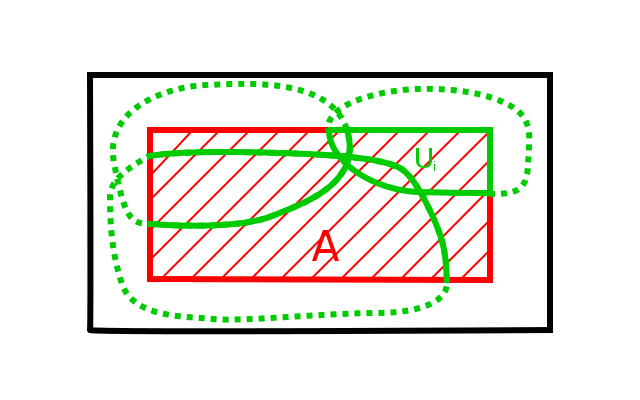
\includegraphics[scale=0.5]{fig27.png}
\caption{}
\end{figure}

Nach Definition der Teilraumtopologie gibt es offene Mengen $V_i$ von $X$, so dass $U_i=V_i\cap A$. Dann ist 
\[
 (X\setminus A) \cup \bigcup_{i\in I} V_i
\]
eine offene Überdeckung von $X$, diese hat eine endliche Teilüberdeckung der Form 
\[
(X\setminus A)\cup V_{i_1} \cup\dotsb \cup V_{i_n}
\]
Somit überdecken die Mengen $U_{i_1}=V_{i_1}\cap A, \dotsc  , U_{i_n}=V_{i_n}\cap A$ ganz $A$.
\end{proof}
\begin{st} \label{thm:1.6.8}
In einem Hausdorffraum sind kompakte Teilräume abgeschlossen.
\end{st}
\begin{proof}
 Sei $X$ ein Hausdorffraum und $A\subset X$ kompakt mit der induzierten Topologie. Wir wollen zeigen, dass es um jeden Punkt $x\in X\setminus A$ eine Umgebung gibt, die A nicht trifft, dann ist $X\setminus A$ offen. Sei $p\in X\setminus A$. Nach der Hausdorffeigenschaft von $X$ finden wir zu jedem $a\in A$ eine offene Umgebung $U_a$ von $a$ und eine offene Umgebung $V_a$ von $p$, so dass $U_a\cap V_a=\emptyset$ gilt. \\
\begin{figure}[h]
\centering
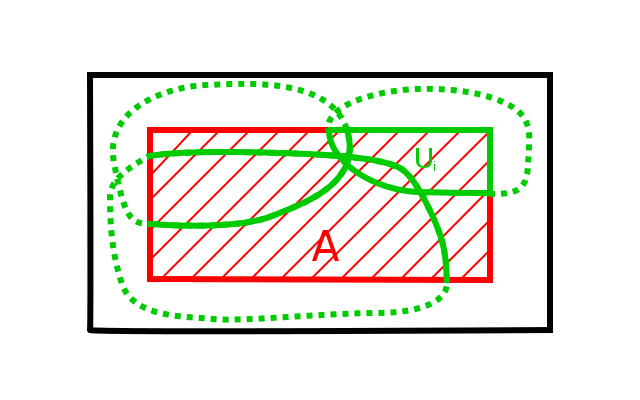
\includegraphics[scale=0.5]{fig28.png}
\caption{}
\end{figure}


\begin{figure}[h]
\centering
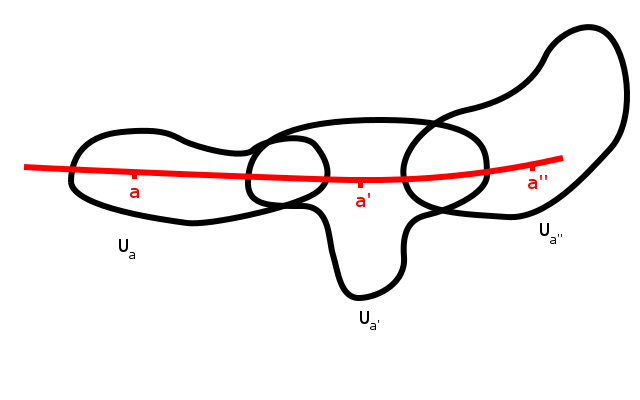
\includegraphics[scale=0.5]{fig29.png}
\caption{}
\end{figure}

Der Schnitt aller $V_a, a\in A$ ist möglicherweise nicht offen (da eventuell Schnittmenge unendlich vieler Mengen), aber da wir wegen der Kompaktheit von $A$ endlich viele Mengen $U_{a_1},\dotsc  , U_{a_n}$ auswählen können, so dass $A\subset U_{a_1}\cup\dotsb \cup U_{a_n}$. Dann gilt: $V_{a_1}\cap\dotsb \cap V_{a_n}$ ist offen und liegt ganz im Komplement von $A$.
\end{proof}
Insgesamt folgt aus Satz \ref{thm:1.6.7} und Satz \ref{thm:1.6.8}, dass in einem kompakten Hausdorffraum \underline{die} Abgeschlossenheit und Kompaktheit von Teilräumen äquivalent sind.
\begin{st}\label{thm:6.8}
 Sei $X$ ein kompakter topologischer Raum und $Y$ ein Hausdorffraum. Sei $f: X\to Y$ eine stetige bijektive Abbildung. Dann ist $f$ ein Homöomorphismus.
\end{st}
\begin{proof}
 Es ist nur zu zeigen, dass $f$ die Eigenschaft hat, dass Bilder offener Mengen offen sind (dann sind die Urbilder offener Mengen unter der Umkehrabbildung $f^{-1}:Y\to X$ offen).

Äquivalent dazu: Die Bilder abgeschlossener Mengen sind abgeschlossen. Sei $A\subset X$ abgeschlossen, da $X$ kompakt, ist A nach \ref{thm:1.6.7} auch kompakt, also ist $f(A)$ nach  \ref{thm:1.6.6}  ein kompakter Teilraum von $Y$. Da $Y$ Hausdorffsch ist, folgt aus \ref{thm:1.6.8}, dass $f(A)$ abgeschlossen ist.
\end{proof}
\begin{ex*}
 \begin{enumerate}[(i)]
  \item Sei $X=\R/\sim$ wie im Beispiel \ref{thm:2.6}, $x\sim y:\iff x-y\in \Z$ und sei $Y=S^1$ (der Einheitskreis in $\R^2$). Dann ist $X=\R/\sim$ kompakt nach \ref{thm:1.6.6}, da Bild der kompakten Teilmenge $[0,1]$ von $\R$. Andererseits ist $Y$ offensichtlich als Teilraum des Hausdorffraums $\R^2$ ebenfalls Hausdorffsch. Die Abbildung $\phi: \R\to Y, t\mapsto e^{i2\pi t}$ (bzw. $(\cos(2\pi t), \sin(2\pi t))^T$) ist stetig, also auch $\bar \phi: \R/\sim \to Y, [t]\mapsto e^{i2\pi t}$, da $\bar \phi$ bijektiv ist, folgt, daraus $\bar \phi$ ein Homöomorphismus ist, insbesondere gilt $\R/\sim \homo S^1$

 \item $S^1=\{(x,y)^T\in \R^2|x^2+y^2=1\}=\{z\in \C||z|=1\}$\\

 Sei $X:=S^1/\sim$ mit $z\sim z':\iff z=z'$ oder $z=-z'$. $X$ ist kompakt, da Bild des kompakten Einheitskreises $S^1$ unter der Quotientenabbildung. Wir wollen zeigen, dass $X\homo S^{1}$ gilt. Definiere $f:X\to S^1$ durch $[z]\mapsto z^2$. Dann ist $f$ wohldefiniert, bijektiv und stetig, da die Abbildung $ f \circ q : S^1 \to S^1, z \mapsto z^2 $ stetig
ist, ($q$ ist die Quotientenabbildung). Nach \ref{thm:6.8} folgt $X\homo S^1$ (bzw. $\R P^1\homo S^1$)
\end{enumerate}
\end{ex*}
Wie bei der Stetigkeit kann man Kompaktheit auch (in gewissen Räumen) durch Folgen beschreiben.
\begin{df}\label{thm:6.9}
 Ein topologischer Raum heißt \emph{folgenkompakt}, wenn jede Folge eine konvergente Teilforge besitzt.  
\end{df}
\begin{ex*}
 Folge $x_n, n\in \N$ sei beschränkte Folge (in $ \R $), dann können wir eine Teilfolge $x_{n_k}$ mit $k \in \N$ auswählen, die monoton ist (also monoton steigend oder monoton fallend). Damit konvergiert diese Teilfolge und die Menge der Folgenglieder ist \emph{kompakt}. Zum Beispiel hat $a_n=(-1)^n+\frac 1 n$ die konvergente Teilfolgen $a_{2n}$ und $a_{2n+1}$
\end{ex*}
\begin{st}\label{thm:6.10}
 In topologischen Räumen, die das zweite Abzählbarkeitsaxiom erfüllen (dass heißt es gibt eine abzählbare Basis der Topologie) sind Folgenkompaktheit und \emph{Überdeckungskompaktheit} (dass heißt Kompaktheit wie in \ref{thm:6.2} defniert) äquivalent.
\end{st}
Zum Beweis benötigen wir zwei Lemmata.
\begin{lem}\label{thm:1.6.12}
 Sei $x_n, n\in \N$, eine Folge in dem topologischen Raum $X$, der das erste Abzählbarkeitsaxiom erfüllt.  Dann gilt: $x_n$ besitzt genau dann eine konvergente Teilfolge, wenn ein $x\in X$ existiert, so dass in jeder Umgebung $U$ von $x$ unendlich viele Folgenglieder $x_n$ liegen.
\end{lem}
\begin{proof}
 \begin{seg}{"`$\implies$"'}
  Gelte $x_{n_k}\to x$ und sei $U$ Umgebung von $x$, dann gibt es $k_0\in \N$, so dass $x_{n_k}\in U$ für $k\ge k_0$.
 \end{seg}
\begin{seg}{"`$\Longleftarrow$"'}
 Sei umgekehrt die obige Bedingung erfüllt und $U_1\supset U_2 \supset \dotsb$ eine Umgebungsbasis von $x$. Wir wählen
$x_{n_1}\in U_1, x_{n_2}\in U_2, \dotsc$ mit $n_1<n_2<\dotsb$. Die letzte Bedingung ist erfüllbar, da im immer unendlich viele Indies $n$ mit $x_n\in U_k, k \in \N$ existieren. Damit ist $x_{n_k}\to x$ offensichtlich.
\end{seg}
\end{proof}
 Wir haben bereits in Lemma \ref{thm:1.6.12} gezeigt. Sei $x_n$ eine Folge in einem topologischen Raum  mit abzählbarer Umgebungsbasis. Dann gilt: $x_n$ besitzt genau dann eine konvergente Teilfolge , wenn ein $x\in X$ existiert, so dass in jeder Umgebung $U$ von $x$ unendlich viele Folgenglieder liegen. Wir wollen nun \ref{thm:6.10} beweisen. Dafür benötigen wir noch ein Lemma.
\begin{lem}\label{thm:6.12}
 Erfüllt $X$ das zweite Abzählbarkeitsaxiom,  so enthält jede offene Überdeckung eine abzählbare Teilüberdeckung
\end{lem}
\begin{proof}
 Sei $O_1,O_2,\dotsc$ eine abzählbare Basis der Topologie. Sei $X=\bigcup_{\alpha\in A} U_\alpha$, $U_\alpha$ 
offen (wir wollen zeigen:  es gibt $\alpha_1, \alpha_2,\dotsc$, so dass $X=\bigcup_{i \in \N} U_{\alpha_i}$). 
Setze $\N'=\{n\in \N|O_n \subset U_\alpha \text{ für ein } \alpha \in A\}$.
Für $n\in \N'$ wählen wir $\alpha_n\in A$ mit $O_n\subset U_{\alpha_n}$. Dann ist $\{U_{\alpha_n}\}_{n\in \N'}$ eine (abzählbare) Überdeckung von $X$. 
Denn jedes $x$ liegt in einem $U_\alpha$. Da die $O_n$ eine Basis bilden ist $U_\alpha$ eine Vereinigung von solchen, also existiert ein $n$ mit $x\in O_n\subset U_{\alpha_n}$, insbesondere $n\in \N'$ und $x\in U_{\alpha_n}$ .
\end{proof}
\begin{seg}{\textbf{Beweis von Satz \ref{thm:6.10}}}
 Sei $X$ ein Raum mit abzählbarer Basis.
\begin{enumerate}[(i)]
 \item Sei $X$ kompakt und $x_n$ eine Folge ohne konvergente Teilfolge. Nach \ref{thm:1.6.12} gibt es zu jedem $p\in X$ eine Umgebung $U_p$ mit $x_n\in U_p$ nur für endlich viele Indizes $n$. Die $U_p$ bilden eine Überdeckung. Wegen der Kompaktheit gibt es endlich viele Mengen $U_{p_1}, \dotsc, U_{p_k}$ die $X$ überdecken. Insgesamt ist $x_n\in U_{p_1}\cup \dotsb \cup U_{p_k}=X$ nur für endlich viele Indizes. Dies ergibt den Widerspruch.
 \item Sei $X$ folgenkompakt und eine offene Überdeckung vorgegeben. Nach \ref{thm:6.12} enthält sie eine abzählbare Teilüberdeckung, etwa $U_1, U_2, \dotsc  $ Können wir aus dieser keine endliche Teilüberdeckung auswählen, dann gilt $X\neq \bigcup_{k=1}^nU_k$ für alle $n \in \N$, dass heißt es gibt $x_n\in X\setminus(U_1\cup\dotsb \cup U_n)$. Wegen Folgenkompaktheit hat $x_n$ eine konvergente Teilfolge $x_{n_k} \to x$ und $x\in U_m$ für ein $m\in \N$. Dann gilt $x_{n_k}\in U_m$ für alle $k$ ab einer Schranke. Dies ergibt den Widerspruch.
\end{enumerate}
\end{seg}
\begin{note*}
 \begin{enumerate}[(i)]
  \item Für die Richtung „kompakt $\implies$ folgenkompakt“ benötigen wir nur das erste Abzählbarkeitsaxiom. 
Insbesondere gilt die Aussage in metrischen Räume.  
(Dies impliziert die Beschränktheit kompakter metrischer Räume). Da metrische Räume und ihre Teilmengen Hausdorff sind, folgt nochmal \ref{thm:1.6.5})
\item Auch Satz \ref{thm:1.6.4} (Heine-Borel) folgt aus dem letzten Satz: Ist $A\subset \R^n$ beschränkt und abgeschlossen, so besitzt jede Folge nach Bolzano eine konvergente Teilfolge.
Also ist $A$ folgenkompakt. Da $\R^n$ (und damit $A$) eine abzählbare Basis (nämlich zum Beispiel $\{B_{n^{-1}} (q)|n\in \N, q\in \Q^n\}$ besitzt,
ist $A$ kompakt. Die andere Richtung folgt aus Bemerkung (i).
\item In einem Banachraum ist die Einheitskugel genau dann kompakt, wenn die Dimension endlich ist,
\item Andererseits: Satz von Tychonoff: Beliebige Produkte kompakter Räume sind kompakt.
 \end{enumerate}
\end{note*}
\subsection{Topologische Mannigfaltigkeiten}
\begin{df}[$n-$dimensionale eingebettete Untermannigfaltigkeit des $\R^{n+k}$]
Eine Teilmenge $M\subset \R^{n+k}$ heißt \emph{$n$-dimensionale Untermannigfaltigkeit} des $\R^{n+k}$, falls es um jeden Punkt $p\in M$ eine (im $\R^{n+k}$) offene Menge, $U$ gibt und einen Diffeomorphismus $\Phi: U\to V$, wobei $V\subset \R^{n+k}$ offen ist und gilt:
\begin{figure}[H]
\centering
 \fixme[fig30]
\caption{}
\end{figure}
\[
 \boxed{\Phi(U\cap M)=V\cap(\R^n\times(\underbrace{0,\dotsc  ,0}_{k-\text{mal}}))}
\]
\end{df}
\begin{exs*}
 \begin{enumerate}[(i)]
  \item offene Mengen im $\R^n$ sind $n-$dimensionale Untermannigfaltigkeit.
  \item lineare (affine) Unterräume (Punkte, Geraden, Ebenen,...) sind Untermannigfaltigkeiten
  \item Die Einheitsphäre $S^n\subset \R^{n+1}$ ist eine $n-$dimensionale Untermannigfaltigkeit
  \item Dass (iii) gilt, zeigt man zum Beispiel, indem man nachrechnet, dass $S^n$ ein \emph{reguläres Urbild} ist. Zum Beispiel ist $S^n$ das Urbild $f^{-1}(\{1\})$ der Abbildung $\R^{n+1}\to \R, (x_1,\dotsc  ,x_{n+1})\mapsto x_1^2+\dotsb +x_{n+1}^2$
 \end{enumerate}
Mannigfaltigkeiten sind Räume, die im Kleinen dem Euklidischen Raum $\R^n$ ähneln, aber nicht notwendig im Großen.
\end{exs*}
\begin{df}
 Ein topologischer Raum M heißt \emph{n-dimensionale topologische Mannigfaltigkeit}, wenn $M$ Hausdorffsch ist, eine abzählbare Basis hat und lokal homöomorph zum $\R^n$ ist, dass heißt für alle $p\in M$ existiert ein Homöomorphismus $\phi:U\to V$, wobei $U$ offene Umgebung von $p$ in $M$ ist und $V$ offen im $\R^n$.
\end{df}
\begin{figure}[H]
\centering
 \fixme[fig31]
\caption{}
\end{figure}
\begin{note*}
 \begin{enumerate}[(i)]
  \item $n-$dimensionale Untermannigfaltigkeit der $\R^{n+k}$ sind $n$-dimensionale topologische Mannigfaltigkeit
  \item Indem wir $\phi$ eventuell einschränken, können wir für $V$ einen offenen Ball nehmen, oder wir können $V$ als $\R^n$ wählen (da offene Bälle im $\R^n$ homöomorph zu $\R^n$ sind, Übungsaufgabe)
  \item Muss lokal aussehen wie $\R^n$. Keine topologische Mannigfaltigkeit sind.
\begin{figure}[H]
\centering
 \begin{tikzpicture}[scale=1, >=triangle 90]
 \begin {scope}
  \draw (3,2.5) -- (3,0.55);
  \draw [densely dashed] (3,0.45) -- (3,0);
  \draw (3,-0.05) -- (3,-1.5);
  \draw (0,0) -- (2,1) -- (6,1) -- (4,0) --cycle;
  \filldraw [red] (3,0.5) circle (1pt);  
 \end {scope}
\begin{scope}[xshift=11cm,yshift=-0.5cm]
  \draw (-1.5,-1.5) -- (2.5,2.5);
  \draw (-1.5,2.5) -- (2.5,-1.5);
  \filldraw [red] (0.5,0.5) circle (1pt);  
\end{scope} 
\end{tikzpicture}



\caption{}
\end{figure}
\item Im Gegensatz zu Untermannigfaltigkeit hat man keine „Glattheitsbedingung“ so ist zum Beispiel ein Quadrat im $\R^2$ eine topologische Mannigfaltigkeit.
 \end{enumerate}
\end{note*}
Es gilt: Die Summe zweier n-dimensionaler topologische Mannigfaltigkeiten ist wieder eine $n$-dimensionale topologische Mannigfaltigkeit. Das Produkt einer $n-$dimensionalen und einer $m$-dimensionalen topologischen Mannigfaltigkeit ist eine $(n+m)$-dimensionale topologische Mannigfaltigkeit.  Offene Teilmengen von $n-$dimensionalen topologischen Mannigfaltigkeiten sind $n$-dimensionale topologische Mannigfaltigkeiten. Für Quotienten von topologischen Mannigfaltigkeit ist die Frage, ob sie wieder topologische Mannigfaltigkeiten sind, kompliziert.
Zum Beispiel:
\begin{figure}[H]
\centering
 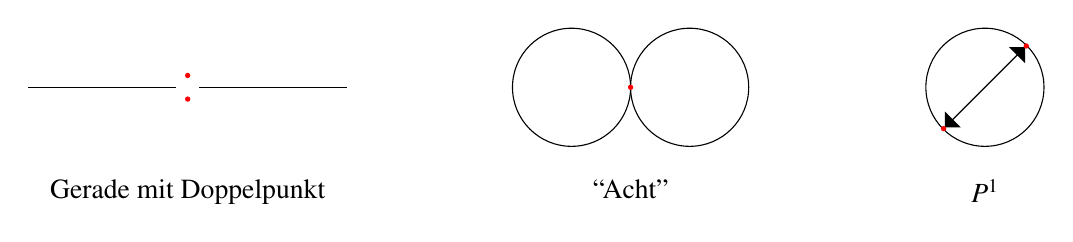
\begin{tikzpicture}[scale=1.5, >=triangle 90]
\begin {scope}[scale=0.5]
  \draw [-] (-0.2,-3) -- (2.3,-3);
  \draw [-] ( 2.7,-3) -- (5.2,-3);
  \filldraw [red] (2.5,-2.8) circle (1pt);
  \filldraw [red] (2.5,-3.2) circle (1pt);
  \draw  (2.5,-4.4) node [anchor=north] {Gerade mit Doppelpunkt};  
\end {scope}
 
\begin {scope}[scale=0.5,xshift=9cm, yshift=-3cm]
 \draw  (0,0) circle (1cm);
 \draw  (2,0) circle (1cm);
 \filldraw [red] (1,0) circle (1pt);
\draw  (1,-1.4) node [anchor=north] {``Acht''};  
\end {scope}

\begin {scope}[scale=0.5,xshift=16cm, yshift=-3cm]
 \draw  (0,0) circle (1cm);
 \draw [<->] (-0.68,-0.68) -- (0.68,0.68);
 \filldraw [red] (0.7,0.7) circle (1pt);
\filldraw [red] (-0.7,-0.7) circle (1pt);
\draw  (0,-1.4) node [anchor=north] {$\R P^1$};  
\end {scope}
\end{tikzpicture}


\caption{}
\end{figure}
Ein Summe von zwei $n$-dimensionalen topologischen Mannigfaltigkeiten ist wieder eine $n$-dimensionale topologische Mannigfaltigeit, das Produkt einer $n$-dimensionalen Mannigfaltigkeit mit einer $m$-dimensionalen Mannigfaltigkeit ist eine $(n+ m)$-dimensionale topologische Mannigfaltigkeit und außerdem sind offene Teilmengen von $n$-dimensionalen topologische Mannigfaltigkeiten wieder $n$-dimensionale topologische Mannigfaltigkeiten.  

Die Konstruktion vom Quotient dagegen ist delikater. Wir begnügen uns mit einem einfachen Fall.

Die Homöomorphismen eines topologischen Raumes $\{\phi: X\to X|\phi \text{ Homöomorphismus}\}$ bilden eine Gruppe, denn die Hintereinanderschaltung von Homöomorphismen ist wieder einer, die Umkehrabbildung eines Homöomorphismus liefert das Inverse, die Identität das neutrale Element.

Wir betrachten (endliche) Untergruppen $\Gamma$ von Homöomorphismen, zum Beispiel $X=S^n, \Gamma=\{\pm \id\}$ , wobei $- \id: S^n\to S^n$ die Antipodenabbildung $x\mapsto -x$ ist. Ist $\Gamma$ eine Gruppe von Homöomorphismen auf $X$, so setzen wir $X/\Gamma:=X/\sim$, wobei die Äquivalenzrelation $\sim$ auf $X$ wie folgt gegeben ist.
\[
 x\sim y :\iff \text{ es gibt ein } \gamma\in \Gamma \text{ mit } y=\underbrace{\gamma(x)}_{:=\gamma x}
\]
\begin{itemize}
\item \emph{reflexiv}, dass heißt $x\sim x$, da $\id_X\in \Gamma$
\item \emph{symmetrisch}, dass heißt $x\sim y \implies y\sim x$, denn falls $y=\gamma(x)$, dann folgt $x=\gamma^{-1}(y)$
\item \emph{transitiv}, dass heißt $x\sim y \land y\sim z \implies x\sim z$, denn $y=\gamma(x), z=\gamma'(y)$, dann folgt $\gamma'\circ \gamma(x)=\gamma' (y)=z$, also $(\gamma'\circ \gamma)(x)=y$. 
\end{itemize}
Dann sind die Äquivalenzklassen die \emph{Bahnen} der Operation von $\Gamma$ auf $X$, wobei die \emph{Bahn} des Punktes $x$ die Menge $\Gamma x:=\{\gamma(x) | \gamma \in \Gamma\}$ ist.

Zum Beispiel falls $X=S^n, \Gamma=\{\pm \id\}$, dann ist $\Gamma x=\{\pm x\}$. Wir versehen $X/\Gamma$ mit der Quotiententopologie. Gilt für $\gamma:X\to X$ und einen Punkt $x\in X$, dass $\gamma(x)=x$, dann nennt man $x$ einen \emph{Fixpunkt} von $\gamma$. Die Identität hat natürlich jeden Punkt als Fixpunkt.
\begin{df}
 Eine Gruppe $\Gamma$ von Homöomorphismen operiert \emph{fixpunktfrei} auf $X$, wenn nur die Identität Fixpunkte auf $X$ hat, dass heißt falls aus $\gamma (x)=x$ für ein $\gamma\in \Gamma$ folgt, dass $\gamma=\id_X$.
\end{df}
\begin{st}\label{thm:7.4}
 Sei $M$ eine $n$-dimensionale topologische Mannigfaltigkeit und $\Gamma$ eine endliche Gruppe von Homöomorphismen, 
die fixpunktfrei auf $M$ operiert. Dann ist $M/\Gamma$ eine $n$-dimensionale topologische Mannigfaltigkeit 
und $\pi:M\to M/\Gamma$ ein lokaler Homöomorphismus. (dass heißt $\forall_{p\in M} \exists$ offene Mengen $U\subset M$ und $V\subset M/\Gamma$ mit $p\in U, V=\pi(U)$ und $\pi\vline_U: U\to V$ Homöomorphismus.)
\end{st}
\begin{proof}
 \begin{enumerate}[(i)]
  \item Die kanonische Projektion (auch: Quotientenabbildung) $\pi:M\to M/\Gamma, p\mapsto [p]=\Gamma p$ ist nicht nur stetig sondern auch offen, dass heißt sie bildet offene Mengen auf offene Mengen ab. Denn ist $U\subset M$ offen, dann ist 
\[
 \pi^{-1}(\pi(U))=\Gamma U=\bigcup\limits_{\gamma\in \Gamma} \underbrace{\gamma(U)}_{\text{offen}}
\]
als Vereinigung von offenen Mengen offen, also ist auch $\pi(U)$ offen.
\item Zu $p\in M$ gibt es eine Umgebung $U$, die keine verschiedenen äquivalenten Punkte enthält, dass heißt $x,\gamma x\in U$ für ein $\gamma\in \Gamma \implies \gamma=\id_x$.
Der Punkt $p$ besitzt eine abzählbare Umgebungsbasis $U_1\supset U_2 \supset U_3 \supset\dotsb $, da $M$ lokal homöomorph zu $\R^n$. Gäbe es in jedem $U_k$ äquivalent verschiedene Elemente, etwa $x_k, \gamma_k x_k\in U_k, \gamma_k\neq \id_X$,
dann könnten wir wegen der Endlichkeit von $\Gamma$ eine Teilfolge $x_{k_l}, \gamma x_{k_l}$ mit konstantem $\gamma\in \Gamma\setminus\{\id\}$ auswählen. Aus $x_{k_l}\to p, \gamma x_{k_l}\to p$ folgt $x_{k_l} \to \gamma^{-1} p$, also $p=\gamma^{-1} p$, also $\gamma=\id_X$ wegen der Fixpunktfreiheit.
\item Auf der Umgebung $U$ aus ii) ist $\pi$ injektiv. Indem wir $U$ eventuell weiter enschränken, können wir annehmen, dass $U$ auch offen ist.  Indem wir $U$ weiter verkleinern, können wir annehmen, dass $U$ homöomorph zu einer offenen Teilmenge des $\R^n$ ist. Wegen (i) ist dann $V:=\pi(U)$ offen und $\pi\vline_U:U\to V$ ein Homöomorphismus.  Insgesamt folgt, dass auch $V\subset M/\Gamma$ homöomorph zu einer offenen Teilmenge das $\R^n$ ist. \\
Noch zu zeigen sind.
\item $M/\Gamma$ ist hausdorffsch und (v) $M/\Gamma$ hat abzählbare Basis, beides als schriftliche Übungsaufgabe.  
\end{enumerate}
\end{proof}
\begin{exs*}
 \begin{enumerate}[(i)]
  \item $M=S^n, \Gamma=\{\pm \id_{S^n}\}, -\id_{S^n}: S^n\to S^n, x\mapsto -x$, die Antipodenabbildung. Da $-\id$ keine Fixpunkte 
auf $S^n$ hat, operiert $\Gamma$ fixpunktfrei auf $S^n$ und $\R P^n := S^n/\{\pm \id\}$ ist eine $n$-dimensionale topologische Mannigfaltigkeit,
 der sogenannte \emph{reell-projektive} Raum der Dimension n. Wir haben bereits gesehen, dass $\R P^1$ homöomorph zu $S^1$ ist, aber für $n \geq 2$ ist $\R P^n$ \emph{nicht} homöomorph zu $S^n$ (Beweis später). Es gibt mehrere Möglichkeiten, den $\R P^n$ (auch $P^n \R, P^n(\R), \dotsc$) zu definieren:
\begin{enumerate}[(i)]
\item $\R P^n=S^n/\{\pm\id\}$ 
\item Als Menge der Geraden in $\R^{n+1}$ durch den Ursprung.
\item Als $\R^{n+1}\setminus \{0\}/\sim$, mit $x\sim y \iff \exists \lambda\in \R\setminus\{0\}: x=\lambda y$. Die Äquivalenzklassen schreibt man als 
\[
[(x_1,\dotsc,x_{n+1})]=[x_1:x_2:\dotsc: x_{n+1}] 
\]
mit $[x_1:\dotsc:x_{n+1}]=[y_1:\dotsc:y_{n+1}]\iff \exists \lambda\in \R\setminus\{0\}$, mit $y_i=\lambda\cdot x_i, \forall_i$.
Gilt $x_3\neq 0$, so gilt $[x_1:x_2:x_3]=[\frac{x_1}{x_3}:\frac{x_2}{x_3}:1]$
\begin{figure}[H]
\centering
 \fixme[fig34]
\caption{}
\end{figure}
\end{enumerate}  
\end{enumerate}
\end{exs*}
\begin{st}
 Für topologische Mannigfaltigkeiten bzw. Abbildungen zwischen diesen sind die folgenden Begriffspaare äquivalent:
\begin{enumerate}[(i)]
 \item Kompaktheit und Folgenkompaktheit
 \item Zusammenhang und Wegzusammenhang
 \item Stetigkeit und Folgenstetigkeit.
\end{enumerate}
\end{st}
\begin{figure}[H]
\centering
 \fixme[fig35]
\caption{}
\end{figure}
\begin{proof}
 (i) und (iii) folgen daraus, dass in topologischen Mannigfaltigkeiten das zweite Abzählbarkeitsaxiom gilt (aus Satz \ref{thm:6.10} bzw. \ref{thm:5.6}(ii))

Bei (ii) gilt $"`\Longleftarrow"'$ stets für alle topologischen Räume. Wir zeigen: Wegzusammenhangskomponenten sind in topologischen Mannigfaltigkeiten offen. Dies gilt wegen der lokalen Homöomorphie zu $\R^n$:
Jeder $\eps$-Ball in $\R^n$ ist wegzusammenhängend, also gibt es um jeden Punkt $p$ in $M$ eine wegzusammenhängende Umgebung.
\end{proof}
\begin{st}[Schwache Version des Whitneyschen Einbettungssatzes]
 Sei $M$ eine kompakte $n$-dimensionale topologische Mannigfaltigkeit. Dann ist $M$ homöomorph zu einer Teilmenge des $\R^N$ für ein $N\in \N$.
\end{st}
\begin{figure}[H]
\centering
 \fixme[fig36]
\caption{}
\end{figure}
\begin{proof}
 Zu jedem Punkt $p\in M$ gibt es einen Homöomorphismus $\phi_p: U_p\to B_2(0) \subset \R^n$ von einer offenen Teilmenge $U_p\ni p$ auf dem offenen $2-$Ball um die Null in $\R^n$. Sei $V_p=\phi_p^{-1}(B_1(0))$. Endlich viele der $V_p$ überdecken $M$, etwa $V_1 \cup \dotsb \cup V_r=M, V_i=V_{p_i}$. Setze $\phi_i:=\phi_{p_i}, U_i=U_{p_i}$. Sei $\lambda:[0,2)\to \R$ eine stetige Funktion mit $\lambda|_{[0,1]}=1$ und $\lambda(x)=0$ für $x>1,5$.
\begin{figure}[H]
\centering
 \begin{tikzpicture}[scale=1, >=triangle 90]
\begin{scope}[scale=2,y=1cm,x=1cm]
\draw[step=.5cm,gray,very thin] (-0.2,-0.2) grid (2.2,1.7);
\draw [-triangle 90] (-0.4,0) -- (2.4,0);
\draw [-triangle 90] (0,-0.4) -- (0,1.9); 
\draw (-0.2,1.9) node [anchor=east] {$Y$};
\draw (2.4,-0.2) node [anchor=north west] {$X$};
\draw [-] (1,0) -- (1,-0.2);
\draw  (1,-0.2) node [anchor=north] {$1$};  
\draw [-] (2,0) -- (2,-0.2);
\draw  (2,-0.2) node [anchor=north] {$2$};  
\path [red,draw] (0,1) -- (1,1) -- (1.5,0) -- (2,0);
\end{scope}
\end{tikzpicture}


\caption{}
\end{figure}
Setze $\tilde \lambda(x)=\lambda(||x||)$ für $x\in B_2(0)$\\
\begin{figure}[H]
\centering
 \fixme[fig38]
\caption{}
\end{figure}
\[
 \tilde \lambda_i(x)=\tilde\lambda \circ \phi_i(x): U_i\to \R
\]
\begin{figure}[H]
\centering
 \fixme[fig39]
\caption{}
\end{figure}
Sei nun 
\[
 \lambda_i: M \to \R, \lambda_i(x):=\begin{cases} \tilde \lambda_i(x)&, x\in U_i\\ 0 &,x \notin U_i \end{cases}
\]
(dass heißt die Forsetzung von $\tilde\lambda_i$ durch $0$ auf ganz $M$). Dann ist $\lambda_i$ stetig, da die Einschränkung von $\lambda_i$ auf die offenen Mengen $U_i$ stetig ist und $M\setminus \underbrace{\phi_i^{-1}(\overline{B_{1,5}(0)})}_{\text{kompakt}}$ offen ist. Definiere $\psi_i: M\to \R^n$ durch $\psi_i(x):= \lambda_i(x)\cdot \phi_i(x)$. Dann ist $\psi_i$ auf ganz $M$ stetig.  Nun können wir den gesuchten Homöomorphismus hinschreiben, definiere $\psi: M\to \R^{r\cdot n+r} , \psi(x)=(\psi_1(x),\dotsc  , \psi_r(x), \lambda_1(x),\dotsc  , \lambda_r(x))$. Die so definierte Abbildung ist offensichtlich stetig, aber auch injektiv, denn wenn $\psi(x)=\psi(y)$ für $x,y\in M$ gibt es $i\in \{1,\dotsc  , r\}$ mit $x\in V_i \implies \lambda_i(x)=1 \implies \lambda_i(y)=1 \implies y \in U_i$. Dann gilt $\phi_i(x)=1\cdot \phi_i(x)=\psi_i(x)=\psi_i(y)=1\cdot \phi_i(y)= \phi_i(y)$, aber $\phi_i$ ist injektiv, also folgt $x=y$. Die Abbildung $\psi$ ist also eine stetige Bijektion von der kompakten Mannigfaltigkeit M auf ihr Bild $\psi(M)$ somit nach Korollar \ref{thm:6.8} ein Homöomorphismus.
\end{proof}
\subsection{Homotopie}
Homotopie ist die Präzisierung der geometrische Idee von der stetigen Deformation einer Abbildung in eine andere.
\begin{df}[Homotopie]
 Seien $X,Y$ topologische Räume und $f_0, f_1: X\to Y$ stetige Abbildungen. Eine \emph{Homotopie} $f$ von $f_0$ nach $f_1$ ist eine parametrisierte Schar von Abbildungen.
$f_t$ mit Anfang $f_0$ und Ende $f_1$, genauer: eine stetige Abbildung $f: X\times[0,1] \to Y$ mit der Eigenschaft, das $f(x,0)=f_0(x)$ und $f(x,1)=f_1(x)$ für alle $x\in X$. (Man schreibt auch $f_t(x)$ für $f(x,t)$)

Wenn es eine Homotopie zwischen $f_0$ und $f_1$ (von $f_0$ nach $f_1$) gibt, dann sagt man $f_0$ und $f_1$ sind \emph{homotop}, Notation: $f_0 \simeq f_1$.
\end{df}
Diese Relation ist eine \emph{Äquivalenzrelation} auf der Menge $C(X,Y)$ der stetigen Abbildung $X\to Y$, denn:
\begin{itemize}
 \item offensichtlich ist jede Abbildung zu sich selbst homotop. Setze $f_t(x):= f(x), \forall_{t \in [0,1]}$. (\emph{reflexiv})
 \item aus einer Homotopie $f$ von $f_0$ nach $f_1$ erhält man die \emph{Inverse Homotopie} $f(\cdot, 1-t)$ von $f_1$ nach $f_0$ (\emph{symmetrisch})
 \item und man kann in offensichtlicher Weise eine Homotopie $f$ von $f_0$ nach $f_1$ mit einer Homotopie $g$ von $f_1$ nach $f_2$ zu einer Homotopie $h$ von $f_0$ nach $f_2$ verknüpfen:
\[
 h(x,t):=\begin{cases}f(x,2t), \text{ falls } t\le 0.5\\ g(x,2t-1), \text{ falls } t>0.5  \end{cases}
\]
dies nennt man das \emph{Produkt} $f*g$ der beiden Homotopien.\\
Die \emph{Äquivalenklasse} $[f]$ einer stetigen Abbildung heißt \emph{Homotopieklasse} von $f$, die Menge der Homotopieklassen stetiger Abbildungen von $X$ nach $Y$ bezeichnen wir mit $[X,Y]$, in Zeichen:
\[
 [X,Y]=C(X,Y)/\simeq
\]
\end{itemize}
\begin{seg}{Zusammenfassung}
 $f_0, f_1: X\to Y$ heißen \emph{homotop}, Notation: $f_0 \simeq f_1,$ falls es ein $f: X\times [0,1] \to  Y$ stetig gibt mit $f(\cdot, 0)=f_0, f(\cdot, 1)=f_1$
\end{seg}

$\simeq$ ist eine Äquivalenzrelation, die Äquivalenzklassen $[X,Y]$ heißen \emph{Homotopieklassen}.  
\begin{exs*}
 \begin{enumerate}
  \item Sei der topologische Raum $X=\{p\}$ einelementig und $Y$ ein beliebiger topoplogischer Raum.  Dann ist eine Homotopie zwischen $f_0: p\mapsto y_0, f_1: p\mapsto y_1$ nichts anderes als ein stetiger Weg von $y_0$ und $y_1$ und $[X,Y]$ steht in 1:1 Relation zu den Wegzusammenhangskomponenten.
  \item Sei $X=S^1, Y=\R^2\setminus \{0\}$. Dann sind nicht alle stetigen Abbildungen $X\to Y$ homotop, denn es lassen sich nicht alle Schleifen (=geschlossene stetige Wege) in $\R^2\setminus\{0\}$   auf einem Punkt zusammenziehen. (Beweis später)
\begin{figure}[H]
\centering
 \fixme[fig40]
\caption{}
\end{figure}
\end{enumerate}
\end{exs*}
\begin{df}
 Eine stetige Abbildung zwischen topologischen Räumen heißt \emph{nullhomotop}, wenn sie zu einer konstanten Abbildung homotop ist. 
\end{df}
\begin{figure}[H]
\centering
 \fixme[fig41]
\caption{}
\end{figure}
\begin{ex*}
 Jede stetige Abbildung nach $\R^n$ ist nullhomotop. Sei $f: X\to \R^n$ stetig, dann ist $f_t(x):= (1-t)\cdot f(x)$ eine Homotopie zur Nullabbildung. 
\end{ex*}
\begin{st}
 Sei $X$ ein topologischer Raum.  Eine stetige Abbildung $S^n\to X$ ist genau dann nullhomotop, wenn sie sich zu einer stetigen Abbildung $\overline{B_1^{n+1}(0)}\to X$ fortsetzen lässt.
\end{st}
\begin{proof}
 \begin{seg}{"`$\Longleftarrow$"'}
  Sei $f: \overline{B_{1}^{n+1}(0)}\to X$ stetig. Definiere die gesuchte Abbildung durch $h(x,t)=f((1-t)x)$.
 \end{seg}
 
\begin{seg}{"`$\implies$"'}
 Sei $h$ eine Homotopie mit $h(\cdot, 0)=f(\cdot)$, mit $f:S^n \to X$ und $h(\cdot, 1)=\const.$
\begin{figure}[H]
\centering
  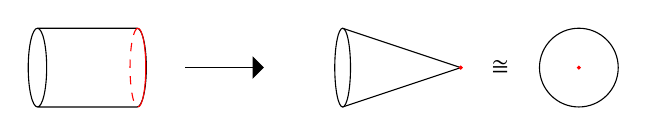
\begin{tikzpicture}[scale=1, >=triangle 90]
\node [cylinder,rotate=180,draw,scale=1,minimum height=1.5cm,minimum width=1cm,aspect=1,anchor=east] at (0,0){}; 
 \draw [red] (1.4,-0.5) arc (-90:90:0.1cm and 0.5cm);
 \draw [red,dashed] (1.4,0.5) arc (90:270:0.1cm and 0.5cm);
 \draw [->] (2,0) -- (3,0);

\begin{scope} [xshift=4cm,scale=0.5]
  \draw (0,0) circle (0.2cm and 1cm);
\draw [-] (0,1) -- (3,0);
\draw [-] (0,-1) -- (3,0);
\filldraw [red] (3,0) circle (1pt);
\end{scope}

\begin{scope}[xshift=7cm,scale=0.5]
 \draw  (-2,0) node [] {$\homo$};  
 \filldraw [red] (0,0) circle (1pt);
\draw  (0,0) circle (1cm);
\end{scope}
\end{tikzpicture}

\caption{}
\end{figure}
Wir betrachten $S^n\times[0,1]$ mit der Äquivalenzrelation $(p,t)\sim (q,s) :\iff (p=q \land t=s) \lor t=s=1$. Dann ist $S^n\times[0,1]/\sim$ homöomorph zu $\overline{B_1^{n+1}(0)}$. Sei $\phi ((p,t)):S^n\times[0,1]\to \overline{B_1^{n+1}(0)}$ mit $(p,t)\mapsto (1-t)\cdot p$, dann ist $\bar \phi: S^n \times[0,1]/\sim \to \overline{B_1^{n+1}(0)}, \bar \phi([(p,t)])=\phi((p,t))$ wohldefiniert, bijektiv und stetig. (Denn $\phi$ ist stetig, $S^n\times [0,1]/\sim$ trägt die Quotiententopologie, $\phi=\bar \phi \circ q $, $q$ die Quotientenabbildung\\
\begin{center}
\makebox{
\begin{xy}
 (0,0)*+{S^n\times [0,1]}; (40,0)*+{\overline{B_{1}^{n+1}(0)}}; (20, -20)*+{S^n\times [0,1]/\sim};
{\ar (10,0)*+{}; (30,0)*+{}}?*!/_2mm/{ \phi};
{\ar (30,-20)*+{}; (40,-1)*+{} }?*!/_2mm/{\bar \phi};
{\ar (0,-1)*+{}; (10,-20)*+{}}?*!/^6mm/{ q};
\end{xy} }
\end{center}

Nach Korollar \ref{thm:6.8} ist $\bar \phi$ ein Homöomorphismus, denn $S^n\times [0,1]/\sim$ ist kompakt und $\overline{B_1^{n+1}(0)}$ ist hausdorffsch. Nun lässt sich $f$ zu der Abbildung $\tilde f: \overline{B_1^{n+1}(0)}\to X, v\mapsto \tilde f(v)$ mit $\tilde f(v):= h(x,t)$,
wobei $(x,t)$ ein Vertreter von $\bar \phi^{-1}(v)$ ist. Mit dem selben Argument wie oben lässt sich zeigen, dass $\tilde f$ stetig ist.
\end{seg}
\end{proof}
\begin{df}
 Eine stetige Abbildung $f: X\to Y$ heißt \emph{Homotopieäquivalenz}, wenn es eine stetige Abbildung $g: Y\to X$ gibt $f\circ g \simeq \id_Y, g\circ f \simeq \id_X$ gilt. Zwei
Räume heißen \emph{homotopieäquivalent} oder vom gleichen \emph{Homotopietyp}, wenn es eine Homotopieäquivalenz gibt. Ein Raum heißt \emph{zusammenziehbar}, wenn er zu einem einpunktigen Raum homotopieäquivalent ist.
\end{df}
\begin{exs*}
 \begin{enumerate}
  \item $\R^n$ ist zusammenziehbar: Sei $f: \R^n\to \{0\}$ und $g:\{0\}\to \R^n, 0 \mapsto 0$. Dann ist $f\circ g=\id_{\{0\}}$ und es gilt $g\circ f(x)=0$ für alle $x\in \R^n$, diese Abbildung ist homotop zu $\id_{\R^n}$, nämlich ist durch $f(x,t):= t\cdot x$ eine Homotopie gegeben.
  \item Eine Teilmenge $K\subset \R^n$ heißt \emph{sternförmig bezüglich} $x_0 \in K$, wenn die Verbindungsstrecke von $x_0$ zu jedem beliebigen Punkt $x\in K$ enthalten ist.\\
\begin{figure}[H]
\centering
 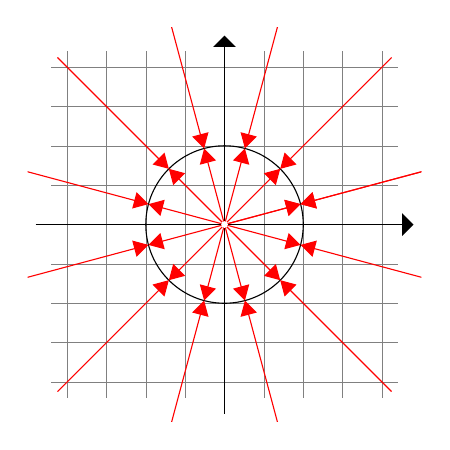
\begin{tikzpicture}[scale=1, >=triangle 60]
\begin{scope}
  \clip (-2.5,-2.5) rectangle (2.5,2.5);
  \draw[step=.5cm,gray,very thin] (-2.2,-2.2) grid (2.2,2.2);
  \draw [-triangle 90] (-2.4,0) -- (2.4,0);
  \draw [-triangle 90] (0,-2.4) -- (0,2.4); 
  \draw   (0,0) circle (1cm);
  \foreach \x in {0,30,...,360}
    {	\draw [red,->] (0,0)	-- (\x+15:1cm);
	\draw [red,->] (0,0)	 ++(\x+15:3cm) -- (\x+15:1cm); 
    }
  \filldraw   [white] (0,0) circle (1pt);
\end{scope}
\end{tikzpicture}

\caption{}
\end{figure}
Sternförmige Mengen sind nullhomotop, denn durch $h: K\times I \to K, (x,t) \mapsto (1-t)x+tx_0$ ist $\id_K$ zu einer konstanten Abbildung homotop. (Allgemein gilt: Ein Raum $X$ ist zusammenziehbar, wenn $\id_X$ nullhomotop ist vgl. 1. )
\item $S^n$ ist homotopieäquivalent zu $\R^{n+1}\setminus\{0\}$ die Inklusionsabbildung $i: S^n\to \R^{n+1}\setminus\{0\}$ ist eine Homotopieäquivalenz:
\begin{figure}[H]
\centering
 \fixme[fig45]
\caption{}
\end{figure}
Denn $n: \R^{n+1}\setminus\{0\} \to S^n, n(x)=\frac{x}{||x||}$ ist das Homotopieinverse zu $i$, durch $h(x,t):=(1-t)n(x)+tx$ ist eine Homotopie von $i\circ n$ zu $\id_{R^{n+1}\setminus \{0\}}$ gegeben.
(In der anderen Richtung gilt ohnehin $n\circ i= \id_{S^n}$)
\end{enumerate}
\end{exs*}
\begin{df}
 Sei $X$ ein topologischer Raum, $A\subset X$ ein Teilraum, $A$ heißt \emph{Retrakt} von $X$, wenn es eine \emph{Retraktion} gibt, das heißt eine stetige Abbildung  $\rho: X\to A$ mit $\rho\vline_A=\id_A$. Ist darüber hinaus $\rho$, aufgefasst als Abbildung $X\to X$, homotop zur Identität auf $X$, so heißt $\rho$ \emph{Deformationsretraktion} und  $A$ \emph{Deformationsretrakt} von $X$.

Eine Deformationsretraktion, so dass die Homotopie $h$ von $\rho$ nach $\id_X$ mit $h(a,t)=a$ für alle $t\in[0,1]$ gewählt werden, heißt \emph{starke Deformationsretraktion}, entsprechend $A$ \emph{starker Deformationsretrakt}.
\end{df}
\begin{note*}
 Alle Beispiele oben sind starke Deformationsretrakte.
\end{note*}
\begin{seg}{Zusammenfassung:}
\begin{itemize}
 \item \emph{Homotopieäquivalenz} $X\simeq Y: \exists f: X\to Y, g: Y\to X, f\circ g \simeq \id_Y, g\circ f \simeq \id_X$
 \item \emph{(Deformations-)Retrakt}:\\
$A\subset X$ heißt \emph{Retrakt}: $\exists f: X\to A, f\vline_A=\id_A$ stetig.
\begin{itemize}
\item \emph{Deformationsretrakt}: $\exists f: X\to A$ homotop zu $\id_X$
\item \emph{starker Deformationsretrakt}: die Homotopie kann so gewählt werden, dass alle Punkte in $A$ während der Deformation fix bleiben.
\begin{figure}[H]
\centering
 \fixme[fig46]
\caption{}
\end{figure}
$A$ und $A'$ sind starke Reformationsretrakte von $X$:
\[
 \implies A \simeq A'
\]
\end{itemize}
\end{itemize}
\end{seg}
\begin{exs*}
\begin{enumerate}[(i)]
 \item 
\begin{seg}{Morsetheorie} 
$M$ differenzierbare Mannigfaltigkeit, $f$ eine differenzierbare Funktion auf $M$. Betrachte Subniveaus $M_a=\{x\in M|f(x)\le a\}$ für $a\in \R$.
 \begin{figure}[H]
\centering
 \fixme[fig47]
\caption{}
\end{figure}
Es gilt: falls für $a<b$ die Funktion $f$ auf $M_b\setminus M_a$ keine kritischen Punkte hat, dann ist $M_a$ ein starker Deformationsretrakt von $M_{b}$
\end{seg}
\begin{proof}[Beweisidee]
 Aus den Gradienten von $f$ kann eine Schar von Diffeomorphismen gewonnen werden, die $M_b$ in $M_a$ deformiert.
\end{proof}
\item $O(n)\subset GL(n, \R)$ ist ein starker Deformationsrektrakt
\begin{proof}
 Durch das Gram-Schmidtsche Orthonormalisierungsverfahren ist eine stetige Abbildung:
\[
 f: GL(n,\R)\to O(n)\times D(n): x\mapsto (f_1(x), f_2(x))
\]
wobei $D(n)$ die Menge der reellen oberen Dreiecksmatrizen mit positiven Diagonalelementen ist. (Es gilt $x=f_1(x)\cdot f_2(x)$)

Die Abbildung $x\mapsto f_1(x)$ ist ein starker Deformationsretrakt, denn durch $h: GL(n,\R)\times [0,1]\to GL(n,\R): (x,t)\mapsto f_1(x)(t\cdot I+(1-t)f_2(x))$, wobei $(1-t)f_2(x)$, die Form:
 \[
  \begin{pmatrix}
   \alpha_1 & * & ...& *\\
 & \ddots & \ddots & \vdots\\
 & & \ddots & *\\
 & & & \alpha_n
  \end{pmatrix}
 \]
ist eine Homotopie von $\id_{GL(n, \R)}$ nach $f_1$ gegeben (bedeute, dass der zweite Faktor in der Definition oben stets invertierbar ist.)
\end{proof}
\end{enumerate}
\end{exs*}
\section{Algebraische Topologie}
\subsection{Die Fundamentalgruppe}
\begin{df}
 Sei $X$ ein topologischer Raum und $x_0, x_1 \in X$. Wir bezeichnen mit
\[
 \Omega(X; x_0,x_1)=\{\omega: [0,1]\to X|\omega \text{ stetig }, \omega(0)=x_0, \omega(1)=x_1 \}
\]
die Menge aller stetigen Wege in $X$ von $x_0$ nach $x_1$. 
\begin{figure}[H]
\centering
 \fixme[fig48]
\caption{}
\end{figure}
Die Menge $\Omega(X; x_0):=\Omega(X; x_0, x_0)$ bezeichnen wir als die Menge aller \emph{Schleifen} mit \emph{Basispunkt} $x_0$.
\end{df}
\begin{df} Für $\omega\in \Omega(X; x_0, x_1)$ und $\nu\in \Omega(X; x_1, x_2)$ sei das \emph{Produkt} $\omega*\nu$ definiert durch:
 \[
  \omega*\nu(t):=\begin{cases} \omega(2t) &\text{ falls } t\in[0,\frac{1}{2})\\ \nu(2t-1) &\text{ falls } t\in[\frac{1}{2}, 1] \end{cases}
 \]
\begin{figure}[H]
\centering
 \fixme[fig49]
\caption{}
\end{figure}
\end{df}
Wir wollen auf dem Raum der Schleifen $\Omega(X; x_0)$ eine Äquivalenzrelation einführen. Dazu benutzen wir eine modifizierte Homotopierelation:
\begin{df}
\begin{figure}[H]
\centering
 \fixme[fig50]
\caption{}
\end{figure}
 Seien $\omega, \nu \in \Omega(X; x_0, x_1)$. Eine \emph{Homotopie mit festen Endpunkten} von $\omega$ nach $\nu$ ist eine stetige Abbildung
\[
 H: [0,1]\times [0,1] \to X,
\]
so dass gilt: 
\begin{align*}
 H(t,0)=\omega(t)&, H(0,s)=x_0\\
 H(t,1)=\nu(t)&, H(1,s)=x_1
\end{align*}
\end{df}
\begin{lem}
 Die Relation $\omega\sim \nu:\iff$ (es gibt eine Homotopie mit festen Endpunkten von $\omega$ nach $\nu$) ist eine Äquivalenzrelation.
\end{lem}
\begin{proof}
 Ist derselbe wie für Homotopie von stetigen Abbildung.
\end{proof}
\begin{lem}  \label{thm:2.1.5}
 Es gilt in $\Omega(X;x_0),$ wobei wir mit $\epsilon$ die \emph{konstante Schleife} 
$\epsilon(t)=x_0 \forall_{t\in [0,1]}$ bezeichnen.
\begin{enumerate}[(i)]
 \item $\omega \sim \omega' \land \nu \sim \nu' \implies \omega *\nu \sim \omega' * \nu'$
  \item $\epsilon * \omega \sim \omega \sim \omega* \epsilon$ 
\item $\omega * \omega^{-1} \sim \epsilon \sim \omega^{-1}*\omega$
 \item $(\omega * \nu)*\xi \sim \omega*(\nu * \xi)$
\end{enumerate}
und wobei wir mit $\omega^{-1}$ den inversen Weg $t\mapsto \omega(1-t)$ bezeichnen.
\end{lem}
\begin{proof}
Wir wollen anhand von Skizzen andeuten wie die Homotopien zu wählen sind.
\fixme[from mathematiker : Nummerierung und Formatierung bitte Überprüfen]
\begin{enumerate}[(i)]
\item .
\begin{figure}[H]
\centering
\begin{tikzpicture} [scale =3]
 \draw (0,0) -- (0,1);
 \draw[color=blue] (0,1) -- (0.5,1);
 \draw[color=red] (0.5,1) -- (1,1);
 \draw (1,0) -- (1,1);
 \draw [color=blue] (0,0) -- (0.5,0);
 \draw [color=red] (0.5,0) -- (1,0);
 \draw [dashed] (0.5,0) -- (0.5,1);
 \draw [blue] (0.25,0.5) node {$f$};
 \draw  [red] (0.75,0.5) node {$g$};
 \draw (0,0) node [anchor=north east] {$0$};
 \draw (0.5,0) node [anchor=north] {$\frac {1}{2}$};
 \draw (1,0) node [anchor=north west] {$1$};
 \draw (0,1) node [anchor=south east] {$1$};
 \draw [blue] (0.25,0) node [anchor=north] {$\omega$};
 \draw [red] (0.75,0) node [anchor=north] {$\nu$};
 \draw [blue] (0.25,1) node [anchor=south] {$\omega'$};
 \draw [red] (0.75,1) node [anchor=south] {$\nu'$};
\end{tikzpicture}
\caption{}
\end{figure}
\item .
\begin{figure}[H]
\centering
\begin{tikzpicture} [scale =3]
 \draw (0,0) rectangle (1,1);
 \draw (0,1) -- (0.5,0); 
 \draw (0,0) node [anchor=north east] {$0$};
 \draw (0.5,0) node [anchor=north] {$\frac {1}{2}$};
 \draw (1,0) node [anchor=north west] {$1$};
 \draw (0,1) node [anchor=south east] {$1$};
 \draw (0.25,0) node [anchor=north] {$\epsilon$};
 \draw (0.75,0) node [anchor=north] {$\omega$};
 \draw (0.5,1) node [anchor=south] {$\omega$};
 \draw (1.5,0.5) node {bzw.};
\begin{scope}[xshift=2cm]
 \draw (0,0) rectangle (1,1);
 \draw (1,1) -- (0.5,0); 
 \draw (0,0) node [anchor=north east] {$0$};
 \draw (0.5,0) node [anchor=north] {$\frac {1}{2}$};
 \draw (1,0) node [anchor=north west] {$1$};
 \draw (0,1) node [anchor=south east] {$1$};
 \draw (0.25,0) node [anchor=north] {$\omega$};
 \draw (0.75,0) node [anchor=north] {$\epsilon$};
 \draw (0.5,1) node [anchor=south] {$\omega$};
\end{scope}
\end{tikzpicture}


\caption{}
\end{figure}
\item .
\begin{figure}[H]
\centering
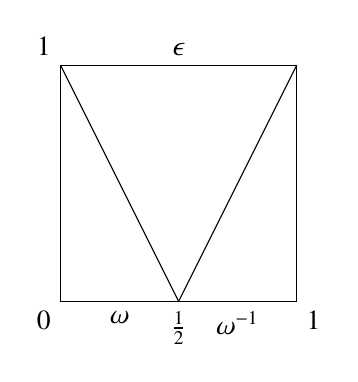
\begin{tikzpicture} [scale =3]
 \draw (0,0) rectangle (1,1);
 \draw (0,1) -- (0.5,0); 
 \draw (1,1) -- (0.5,0); 
 \draw (0,0) node [anchor=north east] {$0$};
 \draw (0.5,0) node [anchor=north] {$\frac {1}{2}$};
 \draw (1,0) node [anchor=north west] {$1$};
 \draw (0,1) node [anchor=south east] {$1$};
 \draw (0.25,0) node [anchor=north] {$\omega$};
 \draw (0.75,0) node [anchor=north] {$\omega^{-1}$};
 \draw (0.5,1) node [anchor=south] {$\epsilon$};
\end{tikzpicture}
\caption{}
\end{figure}
\item .
\begin{figure}[H]
\centering
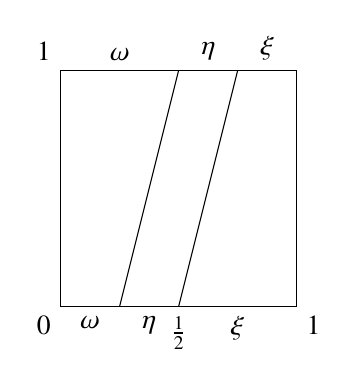
\begin{tikzpicture} [scale =3]
 \draw (0,0) rectangle (1,1);
 \draw (0.25,0) -- (0.5,1); 
 \draw (0.5,0) -- (0.75,1); 
 \draw (0,0) node [anchor=north east] {$0$};
 \draw (0.5,0) node [anchor=north] {$\frac {1}{2}$};
 \draw (1,0) node [anchor=north west] {$1$};
 \draw (0,1) node [anchor=south east] {$1$};
 \draw (0.125,0) node [anchor=north] {$\omega$};
 \draw (0.375,0) node [anchor=north] {$\eta$};
 \draw (0.75,0) node [anchor=north] {$\xi$};
 \draw (0.25,1) node [anchor=south] {$\omega$};
 \draw (0.625,1) node [anchor=south] {$\eta$};
 \draw (0.875,1) node [anchor=south] {$\xi$};
\end{tikzpicture}
\caption{}
\end{figure}
\end{enumerate}
\end{proof}
\begin{note*}[Explizit für (i)]
Sei $f$ die Homotopie zwischen $\omega$ und $\omega'$ und $g$ die Homotopie zwischen $\nu$ und $ \nu'$. Definiere:
\[
 H:[0,1]\times[0,1]\to X
\]
\[
 H(t,s)=\begin{cases} f(2t, s) &\text{ falls } t\in [0, \frac{1}{2}) \\ g(2t-1,s) &\text{ falls } t\in [\frac{1}{2}, 1] \end{cases}
\]
\end{note*}

\begin{df}
 Die Menge der Äquivalenzklassen von Schleifen in $\Omega(X;x_0)$ bezüglich der Relation $\sim$ wird \emph{Fundamentalgruppe} $\pi_1(X; x_0)$ von $(X;x_0)$ genannt, Notation: $\pi_1(X;x_0):= \Omega(X;x_0)/\sim$
\end{df}
Sei:
\[
 \pi_1(X;x_0):= \Omega(X;x_0)/\sim 
\]
wobei $\Omega(X;x_0)$ Schleifen mit Basispunkt $x_0$ und $\sim$ die Homotopie mit festen Endpunkten darstellt.\\
\setcounter{figure}{55} %%% entfernen wenn alle grafiken hochgestellt
\begin{figure}[H]
\centering
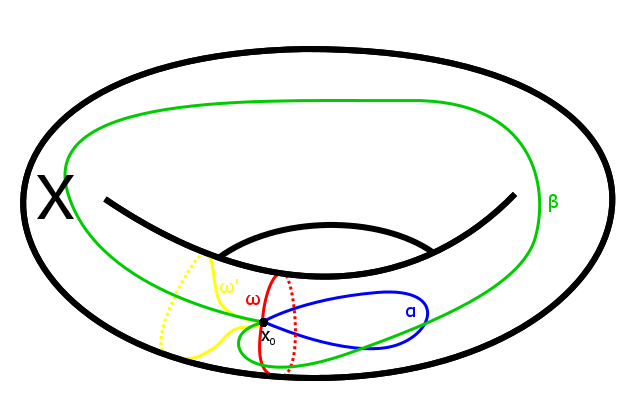
\includegraphics[scale=0.3]{fig56.png}
\caption{}
\end{figure}
Sei $\epsilon$ konstante Schleife $[0,1]\to \{x_0\}$.
Es gilt: $\textcolor {red} {[\omega]}=\textcolor {yellow} {[\omega']}$, $\textcolor {red} {[\omega]}\neq [\epsilon]$, $\textcolor {blue} {[\alpha]}\neq \textcolor {green} {[\beta]}\neq \textcolor {red} {[\omega]}, \textcolor {blue} {[\alpha]}=[\epsilon]$
\begin{st}
 Das Produkt von Schleifen $(\omega, \nu) \mapsto \omega * \nu$ induziert ein Produkt auf $\pi_1(X;x_0)$. Für 
eine Schleife $\omega \in \Omega(X;x_0)$ bezeichne $[\omega] \in \pi_1(X; x_0)$ ihre Homotopieklasse mit festen Endpunkten. Mit diesem Produkt ist $\pi_1(X;x_0)$ eine Gruppe
\end{st}
\begin{proof}
 Seien $\omega, \nu \in \Omega(X; x_0)$. Setze 
\[
 [\omega] \cdot [\nu]:=[\omega*\nu]
\]
Dies ist wohldefiniert, denn nach Lemma \ref{thm:2.1.5} (i) gilt $\omega \sim \omega' \land \nu \sim \nu' \implies \omega * \nu \sim \omega' * \nu'$. Setze weiter $[\omega]^{-1}:=[\omega^{-1}]$, dies ist offensichtlich wohldefiniert, denn $\omega \sim \omega' \implies \omega^{-1}\sim (\omega')^{-1}$. Die Homotopie zwischen $\omega$ und $\omega'$ und $\omega'$ lässt sofort zu einer zwischen den umgekehrt durchlaufenen Schleifen abwandeln. Weiter gilt nach Lemma \ref{thm:2.1.5} (ii) (iii): $\omega*\omega^{-1}\sim \epsilon \sim \omega^{-1}*\omega$ und $\epsilon*\omega\sim \omega \sim \omega*\epsilon$, dies zeigt auch, dass $[\epsilon]$ ein neutrales Element der Multiplikation ist. Teil (iv) von Lemma \ref{thm:2.1.5} liefert die Assoziativität der Verknüpfung. 
\end{proof}
Die so definierte Gruppe $\pi_1(X;x_0)$ ist im Allgemeinen nicht abelsch, wie wir später sehen werden. Die Menge $\Omega(X;x_0)$ bildet \emph{keine} Gruppe mit der Verknüpfung $*$, denn zum Beispiel $\omega*\omega^{-1}\neq \epsilon$, wenn $\omega$ nicht konstant ist.
\begin{exs*}
 \begin{enumerate}[(1)]
  \item Es gilt $\pi_1(\R^n;0)\homo \{1\}$, denn jede Schleife in $\R^n$ mit Basispunkt $0$ kann auf die konstante Schleife $\epsilon: t \mapsto 0$ zusammengezogen werden:

Nämlich ist für $\omega \in \Omega(\R^n;0)$ die Abbildung $H(t,s):=(1-s)\omega(t)$ eine Homotopie zwischen $\omega$ und $\epsilon$. Allgemeiner gilt für jede bezüglich $x_0$ sternförmige Menge $X$, dass $\pi_1(X;x_0)$ trivial ist.
\begin{figure}[H]
\centering
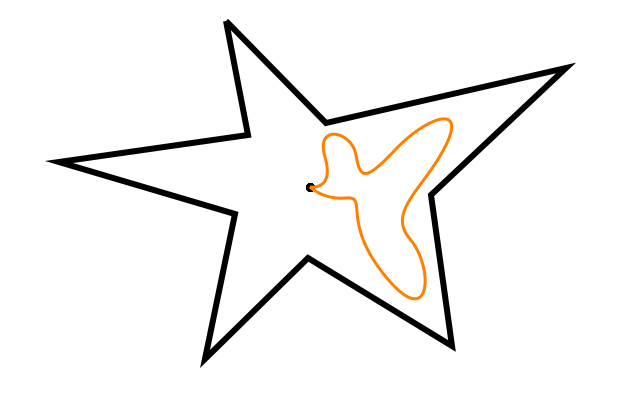
\includegraphics[scale=0.3]{fig57.png}
\caption{}
\end{figure}
\item Es gilt $\pi_1(S^n; p) \homo \{1\}$ für $n\ge 2$ und $p\in S^n$ beliebig.
\begin{figure}[H]
\centering
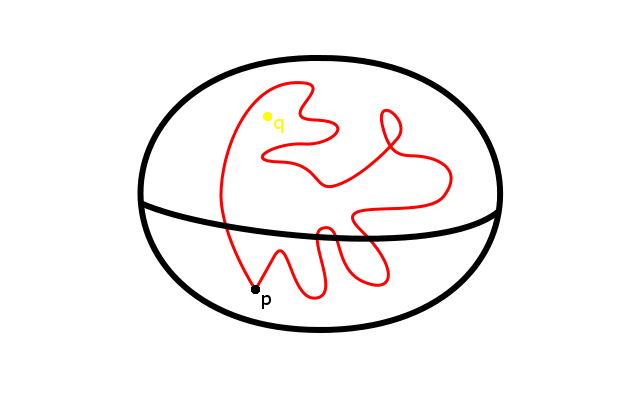
\includegraphics[scale=0.3]{fig58.png}
\caption{}
\end{figure}
\begin{proof}[Beweisskizze]
\begin{figure}[H]
\centering
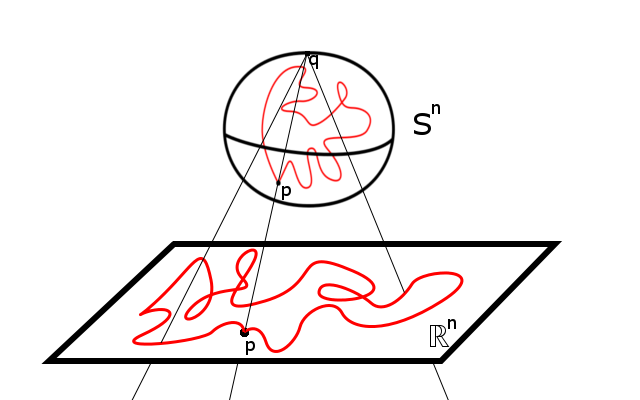
\includegraphics[scale=0.3]{fig59.png}
\caption{}
\end{figure}
 Sei $\omega \in \Omega(S^n;p)$ und sei $q\in S^n\setminus \omega([0,1])$. Dann ist $S^n\setminus\{q\}$ via stereographischer Projektion homöomorph zu $\R^n$ und in $\R^n$ lässt sich jede Schleife zusammenziehen.
\end{proof}
\begin{seg}{Problem bei diesem Beweis}
 Möglicherweise ist $S^n \setminus \omega([0,1])$ \emph{leer}, in der Tat gibt es flächen-/raumfüllende stetige Wege.
\end{seg}

\begin{seg}{Exkurs: flächenfüllende "`Kurve"' (=Weg)}
 Definiere $[0,1] \to A $, wobei $A$ Dreiecksfläche ist, surjektiv wie folgt:

Sei $x\in [0,1]$ und sei zum  Beispiel $x=0,00101\dotsc  $ in Binärdarstellung unterteile das Dreieck rekursiv in kleinere Dreiecke:
\begin{figure}[ht]
\centering
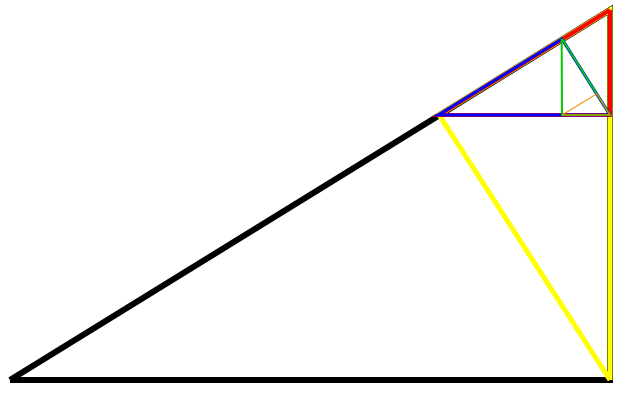
\includegraphics[scale=0.3]{fig60.png}
\caption{}
\end{figure}
Die so entstehende Folge konvergiert gegen einen Limes $f(x)$ und die Abbildung $[0,1]\to A$ ist \emph{surjektiv} und \emph{stetig}.
\end{seg}
\begin{seg}{Lösung}
Ersetze $\omega$ durch einen homotopen nicht surjektiven Weg (Die Konstruktion dieses Weges wird an dieser Stelle nicht gezeigt).
\end{seg}

\item Es gilt: $\pi_1(S^1; 1)\homo \Z$
\begin{proof}[Beweisskizze]
Wir werden diesen Beweis später genauer und allgemeiner im Rahmen der Überlagerungstheorie führen. Der Kreis $S^1=\{ z\in \C| |z|=1\}$ wird von der reellen Geraden $\R$ "`überlagert"': Die Abbildung $p:  \R\to S^1, t\mapsto e^{2\pi i t}$ ist stetig und surjektiv aber \emph{nicht} injektiv.\\
\begin{figure}[ht]
\centering
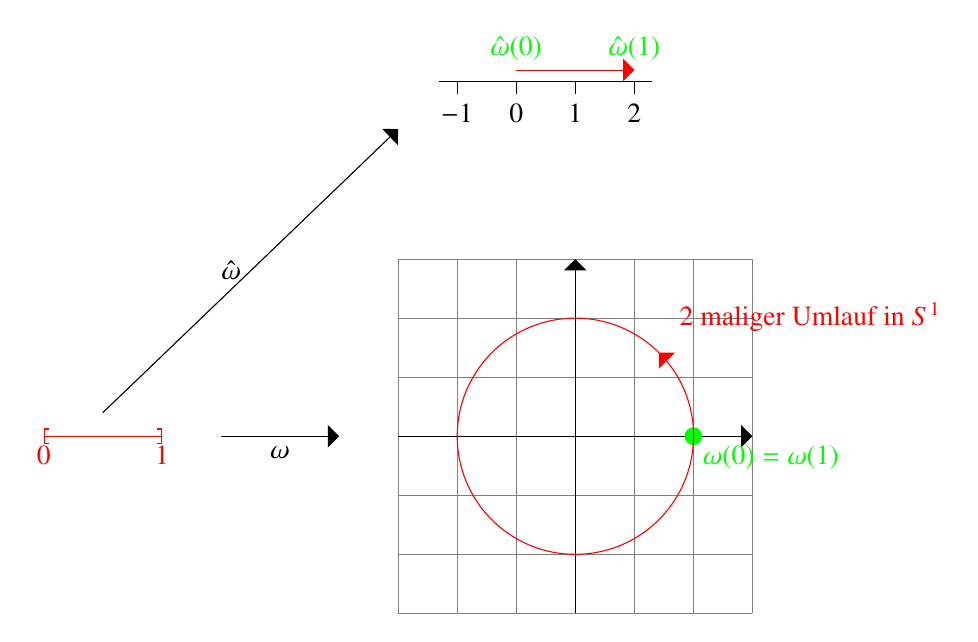
\begin{tikzpicture}[scale=1.5, >=triangle 90]
\begin {scope} [red]
  \draw [[-{]}] (0,0) -- (1,0);
  \draw (0,0) node [anchor=north] {$0$};
  \draw (1,0) node [anchor=north] {$1$};
\end {scope}
\draw [->] (0.5,0.2) -- (3,2.6) node [midway,anchor=east] {$\hat{\omega}$};
\draw [->] (1.5,0) -- (2.5,0) node [midway,anchor=north] {$\omega$};
\begin {scope} [xshift=4cm,yshift=3cm, scale =0.5]
   \draw[step=1cm] (-1.3,-0.2) grid (2.3,0);
  \draw (-1,-0.2) node [anchor=north] {$-1$};
  \draw (0,-0.2) node [anchor=north] {$0$};
  \draw (1,-0.2) node [anchor=north] {$1$};
  \draw (2,-0.2) node [anchor=north] {$2$};
  \draw [red,->](0,0.2) -- (2,0.2);
  \draw [green] (0,0.2) node [anchor=south] {$\hat{\omega} (0)$};
  \draw [green] (2,0.2) node [anchor=south] {$\hat{\omega} (1)$};
\end {scope}
\begin{scope} [xshift=4.5cm,]
\draw[step=.5cm,gray,very thin] (-1.5,-1.5) grid (1.5,1.5);
\draw [->] (-1.5,0) -- (1.5,0);
\draw [->] (0,-1.5) -- (0,1.5); 
\filldraw [green] (1,0) circle (2pt);
\draw [red,->,rotate=45] (1.0cm,0cm) arc (0:360:1.0cm);
\draw [green] (1,0) node [anchor = north west]{$\omega (0) = \omega (1)$};
\draw [red] (0.8,0.8) node [anchor=south west] {2 maliger Umlauf in $S^1$};
\end {scope}
\end{tikzpicture}
\caption{}
\end{figure}
\end{proof}
Wir wollen $\omega$ zu einer Abbildung $\hat\omega$ "`hochheben"' ("`liften"'). Lokal hat $p: \R  \to S^1$ eine Umkehrung (die Argumentfunktion), die aber nicht auf ganz $S^1$ stetig definierbar ist. Sei nun $\omega: [0,1]\to S^1$ eine Schleife, mit $\omega(0)=\omega(1)=1$. Wegen der gleichmäßigen Stetigkeit gibt es eine Unterteilung $0=t_0<t_1<\dotsb <t_k=1$ von $[0,1]$, so dass sich  die Argumentfunktion auf jeden $\omega([t_i, t_{i+1}])$ stetig definieren lässt. Dies liefert einen \emph{Lift} von $\omega$, dass heißt eine Abbildung $\hat \omega: [0,1]\to \R$ mit $p \circ \hat \omega=\omega$. Dieser Lift ist eindeutig(!) bestimmt bis auf die Wahl des Anfangswerts $\hat \omega(0) \in \Z$. Wähle $\hat \omega(0)=0$, dann liefert diese Konstruktion eine Abbildung: $\Omega(S^1, 1)\to \Z, \omega \mapsto \hat \omega(1)$. Aus Stetigkeitsgründen ist diese Abbildung invariant unter Homotopie mit festen Endpunkten, denn es gilt $\hat \omega_S(1)\in \Z$ für eine Homotopie $H(t,s)=\omega_S(t)$. (Später: Auch die Homotopie hat eindeutigen Lift bis auf die Wahl eines Anfangspunktes.) Man überlegt sich \emph{leicht}, dass die so definierte Abbildung additiv ist, dass heißt dass
\[
 f(\omega*\eta)=f(\omega)+f(\eta)
\]
\item Es gilt $\pi_1(\R P^n; p)\homo \Z_2, n\ge 2$
 \begin{table}[h]
  \fixme[Daten hinzufügen]
 \end{table}
\item Für die Linsenräume $L_p$ gilt $\pi_1(L_p;*)\homo \Z_p$ (Beweis später)

\begin{seg}{Challenge}
\begin{figure}[ht]
\centering
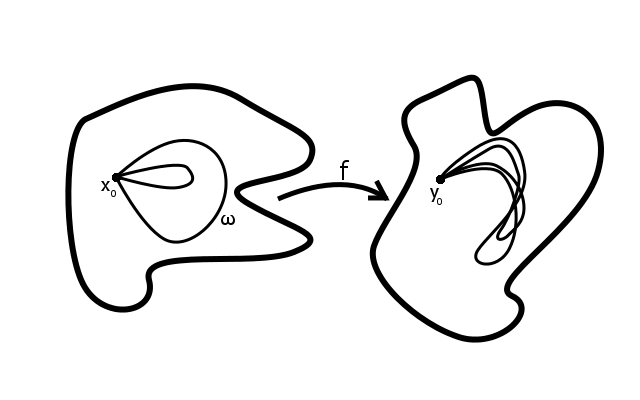
\includegraphics[scale=0.3]{fig62.png}
\caption{}
\end{figure}
$\pi_1("'\infty"'; p) \homo ?$
\fixme[from GnuLinux: bitte Bild überprüfen]
\end{seg}
 \end{enumerate}
\end{exs*}
\begin{seg}{Zusammenfassung}
 Fundamentalgruppe einer "`Acht"':\\
\begin{figure}[H]
\centering
 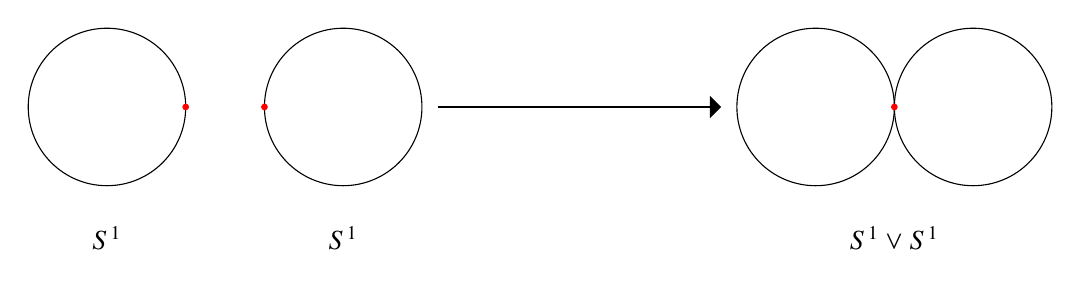
\begin{tikzpicture}[scale=1, >=triangle 90]
\begin {scope}
  \draw  (0,0) circle (1cm);
  \draw  (3,0) circle (1cm);
  \filldraw [red] (1,0) circle (1pt);
  \filldraw [red] (2,0) circle (1pt);
  \draw  (0,-1.4) node [anchor=north] {$S^1$};  
  \draw  (3,-1.4) node [anchor=north] {$S^1$};  
\end {scope}

\draw [->](4.2,0) -- (7.8,0);
 
\begin {scope}[xshift=9cm]
 \draw  (0,0) circle (1cm);
 \draw  (2,0) circle (1cm);
 \filldraw [red] (1,0) circle (1pt);
  \draw  (1,-1.4) node [anchor=north] {$S^1\vee S^1$};  
\end {scope}
\end{tikzpicture}

\caption{}
\end{figure}
\end{seg}
Die \emph{Einpunktvereinigung} oder das \emph{Wedge-Produkt} von zwei Räumen $X$ und $Y$, in denen je ein Punkt $x_0 \in X$ und $y_0\in Y$ ausgezeichnet ist, sei definiert durch 
$$X\lor Y:= (X;x_0) \lor (Y;y_0):=X+Y/{\{x_0,y_0\}} $$
Die "`Acht"' ist also das Wedge-Produkt zweier Kreise $S^1\lor S^1$. Die Fundamentalgruppe von $S^1 \lor S^1$ ist isomorph zu $\Z*\Z$, dem \emph{freien Produkt} der beiden Grupppen. Die Elemente von $\Z*\Z$ sind Worte der Form:
\[
 a^{e_1}\cdot b^{e_2} \cdot a^{e_3} \cdot b^{e_4}\cdot \dotsc \cdot a^{e_{2k-1}}\cdot b^{e_{2k}},
\]
wobei $a$ und $b$ jeweils die Erzeuger einer "`Kopie"' von $\Z$ sind und wobei $e_2, \dotsc, e_{2k-1}\in \Z\setminus\{0\}, e_1, e_{2k} \in \Z$ mit der offensichtlichen Multiplikation (Hintereinanderschreiben und "`Kürzen"'). (Andere Bezeichnung: freie Gruppe in $2$ Erzeugern)

\begin{seg}{Allgemeiner gilt}
 für die Fundamentalgruppe eines Wedge-Produkts:
\[
 \pi_1((X;x_0) \lor (Y;y_0), [x_0])\homo \pi_1(X,x_0)* \pi_1(Y,y_0)
\]
(Beweis später; Satz von Seifert und van Kampen für Fundamentalgruppen von Vereinigungen)
\end{seg}

Wenn wir eine stetige Abbildung zwischen topologischen Räumen haben, können wir die Fundamentalgruppen in Beziehung setzen.
\begin{df}
 Seien $X$ und $Y$ topologische Räume und $x_0\in X, y_0 \in Y$. Eine stetige Abbildung $f: X\to Y$ mit $f(x_0)=y_0$ bezeichnen wir auch als \emph{stetige Abbildung} $(X;x_0)\to (Y;y_0)$. (stetige Abbildungen zwischen "`punktierten"' Räumen) Sei $f: (X;x_0) \to (Y;y_0)$ stetig.  Dann induziert $f$ eine Abbildung:
\[
 \pi_1 (f) : \pi_1(X;x_0)\to \pi_1(Y;y_0), [\omega] \to [f \circ \omega]
\]
\begin{figure}[ht]
\centering



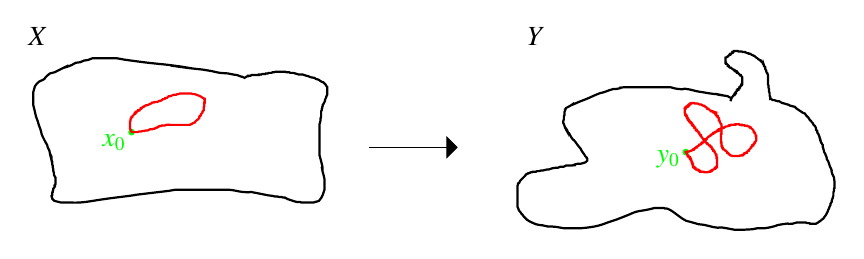
\begin{tikzpicture}[y=0.80pt, x=0.8pt,xscale=0.5,yscale=-0.5, inner sep=0pt, outer sep=0pt]
\begin{scope}
\path [green] (280.3681,688.1819) node [anchor= north east] {$x_0$};
\filldraw [green] (285.3681,686.1819) circle (2pt);

\path[draw=black,line join=miter,line cap=butt,line width=0.800pt]
  (387.3935,637.1895) .. controls (383.2605,635.1230) and (387.4790,637.0496) ..
  (383.3529,635.6743) .. controls (382.4928,635.3876) and (381.7071,634.8840) ..
  (380.8275,634.6641) .. controls (379.6726,634.3754) and (378.4643,634.3659) ..
  (377.2920,634.1590) .. controls (375.6012,633.8606) and (373.9449,633.3618) ..
  (372.2412,633.1489) .. controls (369.8964,632.8558) and (367.5094,632.9780) ..
  (365.1702,632.6438) .. controls (362.7838,632.3029) and (360.4561,631.6336) ..
  (358.0991,631.1286) .. controls (355.0686,630.6235) and (352.0523,630.0248) ..
  (349.0077,629.6133) .. controls (345.8202,629.1826) and (342.6016,629.0122) ..
  (339.4113,628.6032) .. controls (305.7728,624.2906) and (352.0135,629.8228) ..
  (319.7133,625.5727) .. controls (316.5243,625.1531) and (313.3157,624.8993) ..
  (310.1168,624.5626) .. controls (300.0864,623.5068) and (301.7997,623.7501) ..
  (292.4392,622.5423) .. controls (289.5655,622.1715) and (280.7849,621.0009) ..
  (277.7920,620.5220) .. controls (275.9333,620.2246) and (274.1107,619.6822) ..
  (272.2361,619.5118) .. controls (270.3918,619.3442) and (268.5322,619.5118) ..
  (266.6803,619.5118) .. controls (264.6600,619.5118) and (262.6397,619.5118) ..
  (260.6194,619.5118) .. controls (258.4307,619.5118) and (256.2420,619.5118) ..
  (254.0534,619.5118) .. controls (252.7065,619.5118) and (251.3541,619.3899) ..
  (250.0128,619.5118) .. controls (249.4825,619.5600) and (248.9960,619.8300) ..
  (248.4975,620.0169) .. controls (247.6486,620.3352) and (246.8517,620.8072) ..
  (245.9721,621.0271) .. controls (244.8172,621.3158) and (243.6151,621.3638) ..
  (242.4366,621.5321) .. controls (241.2581,622.0372) and (240.1400,622.7170) ..
  (238.9011,623.0474) .. controls (237.5896,623.3971) and (236.1482,623.1232) ..
  (234.8605,623.5524) .. controls (233.5728,623.9817) and (232.5852,625.0686) ..
  (231.3249,625.5727) .. controls (217.1274,631.2518) and (236.7920,622.0113) ..
  (223.7488,628.0981) .. controls (223.7066,628.1178) and (215.6789,632.1345) ..
  (215.6676,632.1387) .. controls (214.3676,632.6262) and (212.8370,632.4682) ..
  (211.6270,633.1489) .. controls (210.0671,634.0263) and (208.9753,635.5559) ..
  (207.5864,636.6844) .. controls (207.2504,638.9076) and (203.1254,639.5250) ..
  (201.5254,640.7250) .. controls (200.6921,641.3500) and (198.5013,643.7428) ..
  (197.9899,644.7656) .. controls (197.6795,645.3865) and (197.6675,646.1162) ..
  (197.4848,646.7859) .. controls (197.1623,647.9684) and (196.6480,649.1081) ..
  (196.4747,650.3215) .. controls (196.3080,651.4881) and (196.4747,652.6785) ..
  (196.4747,653.8570) .. controls (196.4747,654.6988) and (196.4747,655.5406) ..
  (196.4747,656.3824) .. controls (196.4747,658.0660) and (196.2888,659.7599) ..
  (196.4747,661.4332) .. controls (196.6280,662.8130) and (197.1727,664.1210) ..
  (197.4848,665.4738) .. controls (198.1876,668.5193) and (197.9022,668.5267) ..
  (199.0001,672.0398) .. controls (199.4291,673.4127) and (200.0604,674.7157) ..
  (200.5153,676.0804) .. controls (200.9029,677.2431) and (201.1378,678.4531) ..
  (201.5254,679.6159) .. controls (201.9803,680.9805) and (202.6116,682.2835) ..
  (203.0407,683.6565) .. controls (204.4693,688.2282) and (203.4055,686.6356) ..
  (205.0610,690.2225) .. controls (205.6920,691.5897) and (206.3726,692.9344) ..
  (207.0813,694.2631) .. controls (207.7200,695.4608) and (208.5399,696.5630) ..
  (209.1016,697.7986) .. controls (209.3888,698.4306) and (209.3489,699.1744) ..
  (209.6067,699.8189) .. controls (210.0261,700.8676) and (210.7647,701.7780) ..
  (211.1219,702.8494) .. controls (211.4457,703.8209) and (211.4048,704.8802) ..
  (211.6270,705.8799) .. controls (212.7719,711.0323) and (211.3260,703.4617) ..
  (213.1422,708.9103) .. controls (213.3526,709.5417) and (213.0019,710.7342) ..
  (213.1422,711.4357) .. controls (213.2466,711.9578) and (213.5429,712.4289) ..
  (213.6473,712.9509) .. controls (213.8092,713.7603) and (213.4854,714.6669) ..
  (213.6473,715.4763) .. controls (213.7211,715.8455) and (214.0785,716.1173) ..
  (214.1523,716.4865) .. controls (214.2513,716.9817) and (214.0693,717.5035) ..
  (214.1523,718.0017) .. controls (214.2398,718.5268) and (214.5821,718.9899) ..
  (214.6574,719.5169) .. controls (214.6574,724.7944) and (214.4445,718.7442) ..
  (215.1625,723.0525) .. controls (215.2455,723.5507) and (215.0635,724.0724) ..
  (215.1625,724.5677) .. controls (215.2363,724.9368) and (215.4992,725.2411) ..
  (215.6676,725.5778) .. controls (215.8359,725.9146) and (215.9638,726.2748) ..
  (216.1726,726.5880) .. controls (216.3047,726.7861) and (216.6024,726.8672) ..
  (216.6777,727.0931) .. controls (216.7842,727.4125) and (216.6777,727.7665) ..
  (216.6777,728.1032) .. controls (216.6777,728.9450) and (216.6777,729.7868) ..
  (216.6777,730.6286) .. controls (216.6777,730.9799) and (216.7690,732.9713) ..
  (216.6777,733.1540) .. controls (216.5712,733.3669) and (216.2791,733.4461) ..
  (216.1726,733.6591) .. controls (216.0221,733.9602) and (216.4107,734.4311) ..
  (216.1726,734.6692) .. controls (216.0536,734.7883) and (215.7866,734.5502) ..
  (215.6676,734.6692) .. controls (215.6671,734.6697) and (215.6683,736.1822) ..
  (215.6676,736.1844) .. controls (215.5170,736.6362) and (214.8080,736.7428) ..
  (214.6574,737.1946) .. controls (214.5509,737.5140) and (214.7391,737.8781) ..
  (214.6574,738.2047) .. controls (214.5661,738.5700) and (214.2437,738.8497) ..
  (214.1523,739.2149) .. controls (214.0706,739.5416) and (214.2588,739.9056) ..
  (214.1523,740.2251) .. controls (214.0770,740.4509) and (213.6864,740.4953) ..
  (213.6473,740.7301) .. controls (213.5089,741.5605) and (213.7857,742.4252) ..
  (213.6473,743.2555) .. controls (213.3639,744.9554) and (212.4919,742.1694) ..
  (213.1422,744.7707) .. controls (213.2335,745.1360) and (213.5282,745.4237) ..
  (213.6473,745.7809) .. controls (213.7005,745.9406) and (213.5720,746.1354) ..
  (213.6473,746.2860) .. controls (213.7537,746.4989) and (213.9840,746.6227) ..
  (214.1523,746.7910) .. controls (214.4891,747.1278) and (214.8258,747.4645) ..
  (215.1625,747.8012) .. controls (215.3309,747.9696) and (215.4465,748.2178) ..
  (215.6676,748.3063) .. controls (216.3121,748.5641) and (217.0204,748.6206) ..
  (217.6879,748.8113) .. controls (219.5286,749.3373) and (219.4694,749.6161) ..
  (221.7285,749.8215) .. controls (222.7345,749.9130) and (223.7488,749.8215) ..
  (224.7589,749.8215) .. controls (226.7793,749.8215) and (228.7996,749.8215) ..
  (230.8199,749.8215) .. controls (233.1769,749.8215) and (235.5385,749.9685) ..
  (237.8909,749.8215) .. controls (244.4331,749.4126) and (250.0965,748.2685) ..
  (256.5788,747.2961) .. controls (260.1107,746.7663) and (263.6453,746.2529) ..
  (267.1854,745.7809) .. controls (271.2217,745.2427) and (275.2708,744.8038) ..
  (279.3072,744.2657) .. controls (308.7296,740.3427) and (263.1364,745.9561) ..
  (310.6219,740.2251) .. controls (313.4830,739.8797) and (316.3534,739.6087) ..
  (319.2082,739.2149) .. controls (321.2372,738.9350) and (323.2280,738.3748) ..
  (325.2691,738.2047) .. controls (327.2825,738.0370) and (329.3097,738.2047) ..
  (331.3300,738.2047) .. controls (335.0339,738.2047) and (338.7378,738.2047) ..
  (342.4417,738.2047) .. controls (347.9976,738.2047) and (353.5534,738.2047) ..
  (359.1092,738.2047) .. controls (361.2979,738.2047) and (363.4866,738.2047) ..
  (365.6752,738.2047) .. controls (367.8639,738.2047) and (370.0581,738.0488) ..
  (372.2412,738.2047) .. controls (376.8803,738.1639) and (381.2976,739.8586) ..
  (385.8783,740.2251) .. controls (399.2007,741.2908) and (385.8793,738.8679) ..
  (398.5052,741.2352) .. controls (401.8724,741.9086) and (405.2395,742.5821) ..
  (408.6067,743.2555) .. controls (409.9536,743.4239) and (411.3084,743.5374) ..
  (412.6473,743.7606) .. controls (413.3320,743.8747) and (413.9788,744.1796) ..
  (414.6676,744.2657) .. controls (415.3359,744.3492) and (416.0145,744.2657) ..
  (416.6879,744.2657) .. controls (417.3614,744.4340) and (418.0235,744.6566) ..
  (418.7082,744.7707) .. controls (419.3725,744.8814) and (420.0682,744.6387) ..
  (420.7285,744.7707) .. controls (421.2506,744.8751) and (421.7217,745.1714) ..
  (422.2438,745.2758) .. controls (422.5739,745.3418) and (422.9172,745.2758) ..
  (423.2539,745.2758) .. controls (423.4223,745.2758) and (423.6084,745.2005) ..
  (423.7590,745.2758) .. controls (423.9720,745.3823) and (424.0511,745.6744) ..
  (424.2641,745.7809) .. controls (424.4147,745.8562) and (424.6094,745.7277) ..
  (424.7692,745.7809) .. controls (425.4834,746.0190) and (426.0904,746.5114) ..
  (426.7895,746.7910) .. controls (427.7781,747.1865) and (428.8098,747.4645) ..
  (429.8199,747.8012) .. controls (431.3722,748.3186) and (433.2572,749.1371) ..
  (434.8707,749.3164) .. controls (435.7073,749.4094) and (436.5608,749.2120) ..
  (437.3961,749.3164) .. controls (437.9243,749.3824) and (438.3861,749.7340) ..
  (438.9113,749.8215) .. controls (439.4095,749.9045) and (439.9214,749.8215) ..
  (440.4265,749.8215) .. controls (441.7734,749.8215) and (443.1203,749.8215) ..
  (444.4671,749.8215) .. controls (445.4773,749.8215) and (446.4874,749.8215) ..
  (447.4976,749.8215) .. controls (448.1710,749.8215) and (448.8512,749.9167) ..
  (449.5179,749.8215) .. controls (450.0449,749.7462) and (450.5212,749.4627) ..
  (451.0331,749.3164) .. controls (451.4534,749.1963) and (454.0182,748.6365) ..
  (454.5687,748.3063) .. controls (455.3683,747.8265) and (456.1302,746.4691) ..
  (456.5890,745.7809) .. controls (457.8944,743.8227) and (457.4071,744.8415) ..
  (458.1042,742.7504) .. controls (458.6093,741.2352) and (459.2848,739.7665) ..
  (459.6194,738.2047) .. controls (459.7958,737.3816) and (459.6194,736.5212) ..
  (459.6194,735.6794) .. controls (459.6194,734.5009) and (459.6194,733.3223) ..
  (459.6194,732.1438) .. controls (459.6194,730.9653) and (459.7173,729.7827) ..
  (459.6194,728.6083) .. controls (459.4467,726.5356) and (458.5325,724.5460) ..
  (458.1042,722.5474) .. controls (455.4080,709.9653) and (459.0643,726.0099) ..
  (457.5991,716.4865) .. controls (457.3880,715.1143) and (456.9704,713.7808) ..
  (456.5890,712.4459) .. controls (455.9855,710.3339) and (455.2408,709.0624) ..
  (455.0737,706.8900) .. controls (454.9704,705.5471) and (455.0737,704.1963) ..
  (455.0737,702.8494) .. controls (455.0737,699.3139) and (455.0737,695.7783) ..
  (455.0737,692.2428) .. controls (455.0737,689.0440) and (455.0737,685.8452) ..
  (455.0737,682.6464) .. controls (455.0737,681.4678) and (454.9565,680.2835) ..
  (455.0737,679.1108) .. controls (455.1267,678.5811) and (455.4325,678.1075) ..
  (455.5788,677.5956) .. controls (455.7695,676.9281) and (455.9978,676.2641) ..
  (456.0839,675.5753) .. controls (456.0839,670.2978) and (455.8709,676.3480) ..
  (456.5890,672.0398) .. controls (456.6720,671.5415) and (456.5890,671.0296) ..
  (456.5890,670.5245) .. controls (456.5890,670.0194) and (456.5890,669.5144) ..
  (456.5890,669.0093) .. controls (456.5890,668.5042) and (456.4899,667.9893) ..
  (456.5890,667.4941) .. controls (456.6628,667.1249) and (457.0027,666.8491) ..
  (457.0940,666.4839) .. controls (457.1757,666.1573) and (457.0123,665.8004) ..
  (457.0940,665.4738) .. controls (457.1853,665.1085) and (457.5078,664.8288) ..
  (457.5991,664.4636) .. controls (457.6808,664.1369) and (457.5174,663.7801) ..
  (457.5991,663.4535) .. controls (457.6904,663.0882) and (458.0129,662.8085) ..
  (458.1042,662.4433) .. controls (458.1859,662.1166) and (457.9977,661.7526) ..
  (458.1042,661.4332) .. controls (458.1795,661.2073) and (458.4772,661.1262) ..
  (458.6093,660.9281) .. controls (458.8238,660.6062) and (460.0426,658.2252) ..
  (460.1245,657.8976) .. controls (460.2062,657.5710) and (460.0428,657.2141) ..
  (460.1245,656.8875) .. controls (460.3071,656.1570) and (460.8965,655.5814) ..
  (461.1346,654.8672) .. controls (461.1878,654.7074) and (461.0814,654.5218) ..
  (461.1346,654.3621) .. controls (461.3727,653.6478) and (461.9622,653.0722) ..
  (462.1448,652.3418) .. controls (462.2265,652.0151) and (462.1448,651.6683) ..
  (462.1448,651.3316) .. controls (462.1448,650.4898) and (462.1448,649.6480) ..
  (462.1448,648.8062) .. controls (462.1448,647.9645) and (462.1448,647.1227) ..
  (462.1448,646.2809) .. controls (462.1448,645.9441) and (462.2954,645.5719) ..
  (462.1448,645.2707) .. controls (461.9318,644.8448) and (461.4204,644.6415) ..
  (461.1346,644.2606) .. controls (460.9088,643.9594) and (460.8554,643.5516) ..
  (460.6296,643.2504) .. controls (460.3439,642.8695) and (459.9561,642.5770) ..
  (459.6194,642.2403) .. controls (459.2827,641.9035) and (459.0176,641.4751) ..
  (458.6093,641.2301) .. controls (458.1527,640.9562) and (457.5702,640.9631) ..
  (457.0940,640.7250) .. controls (456.0082,640.1821) and (455.1795,639.1830) ..
  (454.0636,638.7047) .. controls (453.4255,638.4313) and (452.6813,638.4731) ..
  (452.0433,638.1996) .. controls (451.4853,637.9605) and (451.1039,637.3814) ..
  (450.5280,637.1895) .. controls (449.5565,636.8656) and (448.4856,636.9539) ..
  (447.4976,636.6844) .. controls (446.6229,636.4459) and (445.8323,635.9610) ..
  (444.9722,635.6743) .. controls (444.3137,635.4547) and (443.6168,635.3687) ..
  (442.9519,635.1692) .. controls (441.9320,634.8632) and (440.9739,634.3209) ..
  (439.9214,634.1590) .. controls (438.7566,633.9798) and (437.5586,634.2763) ..
  (436.3859,634.1590) .. controls (435.8561,634.1060) and (435.3806,633.8069) ..
  (434.8707,633.6540) .. controls (433.6967,633.3018) and (432.5441,632.8453) ..
  (431.3351,632.6438) .. controls (430.5048,632.5054) and (429.6431,632.7629) ..
  (428.8098,632.6438) .. controls (428.4371,632.5906) and (428.1688,632.2126) ..
  (427.7996,632.1387) .. controls (426.9742,631.9736) and (426.0909,632.3429) ..
  (425.2742,632.1387) .. controls (424.9090,632.0474) and (424.6212,631.7527) ..
  (424.2641,631.6337) .. controls (424.1044,631.5805) and (423.9274,631.6337) ..
  (423.7590,631.6337) .. controls (423.4223,631.6337) and (423.0856,631.6337) ..
  (422.7488,631.6337) .. controls (421.9071,631.6337) and (421.0653,631.6337) ..
  (420.2235,631.6337) .. controls (419.0450,631.6337) and (417.8664,631.6337) ..
  (416.6879,631.6337) .. controls (416.3512,631.6337) and (416.0145,631.6337) ..
  (415.6778,631.6337) .. controls (415.5094,631.6337) and (415.3324,631.5805) ..
  (415.1727,631.6337) .. controls (414.8156,631.7527) and (414.5278,632.0474) ..
  (414.1625,632.1387) .. controls (413.6726,632.2612) and (413.1265,631.9790) ..
  (412.6473,632.1387) .. controls (412.2902,632.2578) and (411.9943,632.5248) ..
  (411.6372,632.6438) .. controls (411.3638,632.7349) and (409.7889,632.6438) ..
  (409.6169,632.6438) .. controls (407.9910,632.6438) and (410.4791,632.5248) ..
  (408.6067,633.1489) .. controls (407.9678,633.3618) and (407.2253,632.9359) ..
  (406.5864,633.1489) .. controls (406.3605,633.2242) and (406.3123,633.5962) ..
  (406.0813,633.6540) .. controls (405.2647,633.8581) and (404.3726,633.4498) ..
  (403.5559,633.6540) .. controls (403.1907,633.7453) and (402.9110,634.0677) ..
  (402.5458,634.1590) .. controls (402.1709,634.2527) and (400.6805,634.0040) ..
  (400.5255,634.1590) .. controls (400.4064,634.2781) and (400.6445,634.5451) ..
  (400.5255,634.6641) .. controls (400.5093,634.6804) and (399.1328,634.6641) ..
  (399.0103,634.6641) .. controls (397.6634,634.6641) and (396.3165,634.6641) ..
  (394.9697,634.6641) .. controls (394.4646,634.6641) and (393.9336,634.5044) ..
  (393.4544,634.6641) .. controls (393.2285,634.7394) and (393.1623,635.0627) ..
  (392.9493,635.1692) .. controls (392.6005,635.3436) and (390.6013,634.9919) ..
  (390.4240,635.1692) .. controls (390.3049,635.2882) and (390.5430,635.5552) ..
  (390.4240,635.6743) .. controls (390.3049,635.7933) and (390.0695,635.5990) ..
  (389.9189,635.6743) .. controls (389.0408,636.1133) and (388.2353,636.6844) ..
  (387.3935,637.1895) -- cycle;
\path[draw=red,line join=miter,line cap=butt,line width=0.800pt]
  (285.3681,686.1819) .. controls (286.7150,686.1819) and (288.0618,686.1819) ..
  (289.4087,686.1819) .. controls (289.7454,686.1819) and (290.0821,686.1819) ..
  (290.4189,686.1819) .. controls (290.5872,686.1819) and (290.7642,686.2351) ..
  (290.9239,686.1819) .. controls (291.2811,686.0628) and (291.5689,685.7681) ..
  (291.9341,685.6768) .. controls (292.5874,685.5135) and (293.3011,685.8401) ..
  (293.9544,685.6768) .. controls (294.3196,685.5855) and (294.5993,685.2630) ..
  (294.9645,685.1717) .. controls (295.6179,685.0084) and (296.3315,685.3351) ..
  (296.9848,685.1717) .. controls (297.3501,685.0804) and (297.6237,684.7285) ..
  (297.9950,684.6667) .. controls (298.6593,684.5559) and (299.3620,684.8300) ..
  (300.0153,684.6667) .. controls (300.7457,684.4840) and (301.3213,683.8946) ..
  (302.0356,683.6565) .. controls (302.6745,683.4435) and (303.4026,683.8198) ..
  (304.0559,683.6565) .. controls (304.4211,683.5652) and (304.7009,683.2427) ..
  (305.0661,683.1514) .. controls (305.3927,683.0697) and (305.7568,683.2579) ..
  (306.0762,683.1514) .. controls (306.3021,683.0761) and (306.3832,682.7784) ..
  (306.5813,682.6463) .. controls (306.8945,682.4375) and (307.2343,682.2603) ..
  (307.5915,682.1413) .. controls (309.0950,681.6401) and (306.5551,683.3372) ..
  (309.1067,681.6362) .. controls (309.3048,681.5041) and (309.3988,681.2376) ..
  (309.6118,681.1311) .. controls (309.7623,681.0558) and (309.9663,681.2064) ..
  (310.1168,681.1311) .. controls (310.3298,681.0246) and (310.4090,680.7325) ..
  (310.6219,680.6260) .. controls (311.0260,680.4240) and (311.7331,680.8281) ..
  (312.1371,680.6260) .. controls (312.3501,680.5196) and (312.4293,680.2274) ..
  (312.6422,680.1210) .. controls (312.7928,680.0457) and (312.9789,680.1210) ..
  (313.1473,680.1210) .. controls (313.4840,680.1210) and (313.8207,680.1210) ..
  (314.1574,680.1210) .. controls (314.4942,680.1210) and (314.8309,680.1210) ..
  (315.1676,680.1210) .. controls (315.3360,680.1210) and (315.5130,680.1742) ..
  (315.6727,680.1210) .. controls (316.0298,680.0019) and (316.3176,679.7072) ..
  (316.6828,679.6159) .. controls (317.0246,679.5304) and (319.8933,679.6159) ..
  (320.2184,679.6159) .. controls (323.0805,679.6159) and (325.9426,679.6159) ..
  (328.8047,679.6159) .. controls (330.9933,679.6159) and (333.1820,679.6159) ..
  (335.3707,679.6159) .. controls (335.7936,679.6159) and (337.5119,679.7119) ..
  (337.8960,679.6159) .. controls (338.2613,679.5246) and (338.5490,679.2299) ..
  (338.9062,679.1108) .. controls (339.0659,679.0576) and (339.2607,679.1861) ..
  (339.4113,679.1108) .. controls (339.6242,679.0043) and (339.7182,678.7378) ..
  (339.9163,678.6057) .. controls (340.2296,678.3969) and (340.5898,678.2690) ..
  (340.9265,678.1007) .. controls (341.2632,677.9323) and (341.5795,677.7146) ..
  (341.9366,677.5956) .. controls (342.0964,677.5424) and (342.3227,677.7146) ..
  (342.4417,677.5956) .. controls (342.7079,677.3294) and (342.7380,676.8987) ..
  (342.9468,676.5854) .. controls (343.0789,676.3873) and (343.2835,676.2487) ..
  (343.4519,676.0804) .. controls (343.6202,675.9120) and (343.7588,675.7073) ..
  (343.9569,675.5753) .. controls (344.2702,675.3665) and (344.6539,675.2790) ..
  (344.9671,675.0702) .. controls (345.1652,674.9381) and (345.3038,674.7335) ..
  (345.4722,674.5651) .. controls (345.6405,674.3968) and (345.8452,674.2582) ..
  (345.9773,674.0600) .. controls (347.0900,673.8057) and (346.2442,673.0210) ..
  (346.4823,672.5448) .. controls (346.5888,672.3319) and (346.8809,672.2527) ..
  (346.9874,672.0397) .. controls (347.0627,671.8892) and (346.8684,671.6537) ..
  (346.9874,671.5347) .. controls (347.2536,671.2685) and (347.7887,671.3428) ..
  (347.9976,671.0296) .. controls (348.1843,670.7494) and (347.8911,670.3389) ..
  (347.9976,670.0194) .. controls (348.1474,669.5699) and (349.3629,668.9538) ..
  (349.5128,668.5042) .. controls (349.6193,668.1848) and (349.4063,667.8135) ..
  (349.5128,667.4941) .. controls (349.6634,667.0423) and (350.3100,666.9098) ..
  (350.5229,666.4839) .. controls (350.6763,666.1772) and (350.3696,663.7601) ..
  (350.5229,663.4534) .. controls (350.6294,663.2405) and (350.9215,663.1613) ..
  (351.0280,662.9484) .. controls (351.1049,662.7947) and (351.0280,661.6606) ..
  (351.0280,661.4331) .. controls (351.0280,661.2477) and (351.0077,659.4332) ..
  (351.0280,659.4128) .. controls (351.1471,659.2938) and (351.4140,659.5319) ..
  (351.5331,659.4128) .. controls (351.5560,659.3899) and (351.5331,657.1256) ..
  (351.5331,656.8875) .. controls (351.5331,656.7191) and (351.6521,656.5014) ..
  (351.5331,656.3824) .. controls (351.4140,656.2633) and (351.1471,656.5014) ..
  (351.0280,656.3824) .. controls (350.9090,656.2633) and (351.1471,655.9964) ..
  (351.0280,655.8773) .. controls (350.9090,655.7583) and (350.6735,655.9526) ..
  (350.5229,655.8773) .. controls (350.3100,655.7708) and (350.2160,655.5043) ..
  (350.0179,655.3722) .. controls (349.7046,655.1634) and (349.3209,655.0760) ..
  (349.0077,654.8672) .. controls (348.8096,654.7351) and (348.7007,654.4941) ..
  (348.5026,654.3621) .. controls (348.1894,654.1533) and (347.8292,654.0254) ..
  (347.4925,653.8570) .. controls (347.1558,653.6886) and (346.8319,653.4917) ..
  (346.4823,653.3519) .. controls (345.9880,653.1542) and (345.4614,653.0446) ..
  (344.9671,652.8468) .. controls (343.6202,652.3081) and (344.1168,652.1717) ..
  (342.4417,651.8367) .. controls (341.7814,651.7046) and (341.0747,652.0000) ..
  (340.4214,651.8367) .. controls (340.0562,651.7454) and (339.7765,651.4229) ..
  (339.4113,651.3316) .. controls (339.0846,651.2499) and (338.7378,651.3316) ..
  (338.4011,651.3316) .. controls (338.0644,651.3316) and (337.7277,651.3316) ..
  (337.3910,651.3316) .. controls (336.0441,651.3316) and (334.6972,651.3316) ..
  (333.3503,651.3316) .. controls (332.0694,651.3316) and (329.8769,651.1784) ..
  (328.8047,651.3316) .. controls (328.4320,651.3848) and (328.1597,651.7454) ..
  (327.7945,651.8367) .. controls (327.4678,651.9184) and (327.1110,651.7550) ..
  (326.7844,651.8367) .. controls (326.4191,651.9280) and (326.1394,652.2505) ..
  (325.7742,652.3418) .. controls (325.1209,652.5051) and (324.4143,652.2097) ..
  (323.7539,652.3418) .. controls (322.7137,652.5498) and (322.1264,652.9030) ..
  (321.2285,653.3519) .. controls (320.8918,653.5203) and (320.5875,653.7832) ..
  (320.2184,653.8570) .. controls (319.7231,653.9561) and (319.1931,653.7345) ..
  (318.7031,653.8570) .. controls (318.4721,653.9148) and (318.3664,654.1937) ..
  (318.1981,654.3621) .. controls (317.8613,654.6988) and (317.6300,655.1954) ..
  (317.1879,655.3722) .. controls (316.7190,655.5598) and (316.1244,655.1464) ..
  (315.6727,655.3722) .. controls (315.3360,655.5406) and (315.4338,656.1162) ..
  (315.1676,656.3824) .. controls (315.1671,656.3829) and (313.6547,656.3816) ..
  (313.6524,656.3824) .. controls (313.4265,656.4577) and (313.3157,656.7191) ..
  (313.1473,656.8875) .. controls (312.6339,657.4009) and (312.4475,657.6938) ..
  (311.6321,657.8976) .. controls (311.3054,657.9793) and (310.9486,657.8159) ..
  (310.6219,657.8976) .. controls (309.8915,658.0802) and (309.3159,658.6697) ..
  (308.6016,658.9078) .. controls (308.1176,659.0691) and (306.5441,658.7518) ..
  (306.0762,658.9078) .. controls (305.8503,658.9831) and (305.7841,659.3064) ..
  (305.5712,659.4128) .. controls (305.1671,659.6149) and (304.4600,659.2108) ..
  (304.0559,659.4128) .. controls (303.6300,659.6258) and (303.4717,660.2100) ..
  (303.0458,660.4230) .. controls (302.8952,660.4983) and (302.7004,660.3698) ..
  (302.5407,660.4230) .. controls (301.8264,660.6611) and (301.1938,661.0964) ..
  (300.5204,661.4331) .. controls (300.1837,661.6015) and (299.8755,661.8469) ..
  (299.5102,661.9382) .. controls (299.1836,662.0199) and (298.8267,661.8565) ..
  (298.5001,661.9382) .. controls (296.0611,662.5480) and (298.5251,662.1782) ..
  (296.9849,662.9484) .. controls (296.8343,663.0237) and (296.6304,662.8731) ..
  (296.4798,662.9484) .. controls (296.2668,663.0549) and (296.1877,663.3470) ..
  (295.9747,663.4534) .. controls (295.8241,663.5287) and (295.6202,663.3781) ..
  (295.4696,663.4534) .. controls (295.0437,663.6664) and (294.8854,664.2506) ..
  (294.4595,664.4636) .. controls (294.3089,664.5389) and (294.0734,664.3446) ..
  (293.9544,664.4636) .. controls (292.9094,665.5086) and (295.5513,664.4227) ..
  (293.4493,665.4738) .. controls (292.7526,665.8221) and (292.9975,664.8621) ..
  (292.4392,665.9788) .. controls (292.3639,666.1294) and (292.5582,666.3649) ..
  (292.4392,666.4839) .. controls (292.2011,666.7220) and (291.6671,666.2458) ..
  (291.4290,666.4839) .. controls (291.3100,666.6030) and (291.5481,666.8699) ..
  (291.4290,666.9890) .. controls (291.3100,667.1080) and (291.0745,666.9137) ..
  (290.9239,666.9890) .. controls (290.7110,667.0955) and (290.6318,667.3876) ..
  (290.4189,667.4941) .. controls (290.2683,667.5694) and (290.0328,667.3750) ..
  (289.9138,667.4941) .. controls (289.7947,667.6131) and (290.0328,667.8801) ..
  (289.9138,667.9991) .. controls (289.7947,668.1182) and (289.5278,667.8801) ..
  (289.4087,667.9991) .. controls (289.2897,668.1182) and (289.5278,668.3852) ..
  (289.4087,668.5042) .. controls (289.2897,668.6233) and (289.0227,668.3852) ..
  (288.9036,668.5042) .. controls (288.7846,668.6233) and (289.0227,668.8902) ..
  (288.9036,669.0093) .. controls (288.7846,669.1283) and (288.5176,668.8902) ..
  (288.3986,669.0093) .. controls (288.2795,669.1283) and (288.5176,669.3953) ..
  (288.3986,669.5144) .. controls (288.2795,669.6334) and (288.0125,669.3953) ..
  (287.8935,669.5144) .. controls (287.7744,669.6334) and (287.9688,669.8689) ..
  (287.8935,670.0194) .. controls (287.6450,670.5164) and (286.1217,671.5427) ..
  (285.8732,672.0397) .. controls (285.7979,672.1903) and (285.9922,672.4258) ..
  (285.8732,672.5448) .. controls (285.7541,672.6639) and (285.4871,672.4258) ..
  (285.3681,672.5448) .. controls (285.2491,672.6639) and (285.4434,672.8993) ..
  (285.3681,673.0499) .. controls (285.2616,673.2629) and (284.9695,673.3420) ..
  (284.8630,673.5550) .. controls (284.7877,673.7056) and (284.9383,673.9095) ..
  (284.8630,674.0600) .. controls (284.7565,674.2730) and (284.4644,674.3522) ..
  (284.3579,674.5651) .. controls (284.1559,674.9692) and (284.5600,675.6763) ..
  (284.3579,676.0804) .. controls (284.2515,676.2933) and (283.9593,676.3725) ..
  (283.8529,676.5854) .. controls (283.7760,676.7391) and (283.8529,677.8732) ..
  (283.8529,678.1007) .. controls (283.8529,679.1108) and (283.8529,680.1210) ..
  (283.8529,681.1311) .. controls (283.8529,681.3952) and (283.7865,683.0186) ..
  (283.8529,683.1514) .. controls (283.9593,683.3644) and (284.1896,683.4881) ..
  (284.3579,683.6565) .. controls (284.6947,684.4983) and (285.0314,685.3401) ..
  (285.3681,686.1819) -- cycle;
\end{scope}
\draw (200,600) node {$X$};
\draw (650,600) node {$Y$};
\draw [-triangle 90] (500,700)  -- (580,700);
\begin{scope}[xshift=350, yshift=90]
  \path [green] (343.5026,589.7326) node [anchor= north east] {$y_0$};
  \filldraw [green] (348.5026,591.7326) circle (2pt);

\path[draw=black,line join=miter,line cap=butt,line width=0.800pt]
  (389.9189,542.7402) .. controls (389.2455,542.5719) and (388.5720,542.4035) ..
  (387.8986,542.2351) .. controls (387.3935,541.8984) and (386.9592,541.4169) ..
  (386.3834,541.2250) .. controls (385.7573,541.0163) and (380.2065,540.2927) ..
  (379.8174,540.2148) .. controls (366.8286,537.6171) and (386.7285,540.8528) ..
  (370.2209,538.6996) .. controls (368.1899,538.4347) and (366.1803,538.0262) ..
  (364.1600,537.6895) .. controls (362.1397,537.3527) and (360.1042,537.0970) ..
  (358.0991,536.6793) .. controls (356.0604,536.2546) and (354.0899,535.5209) ..
  (352.0382,535.1641) .. controls (341.8469,533.3917) and (351.0206,535.6684) ..
  (341.4316,534.6590) .. controls (339.1010,534.9148) and (337.0980,533.3918) ..
  (334.8656,533.1438) .. controls (334.0289,533.0508) and (333.1820,533.1438) ..
  (332.3402,533.1438) .. controls (330.3199,533.1438) and (328.2996,533.1438) ..
  (326.2793,533.1438) .. controls (321.7336,533.1438) and (317.1879,533.1438) ..
  (312.6422,533.1438) .. controls (308.2649,533.1438) and (303.8876,533.1438) ..
  (299.5102,533.1438) .. controls (297.9950,533.1438) and (296.4798,533.1438) ..
  (294.9645,533.1438) .. controls (294.2911,533.1438) and (293.6149,533.0828) ..
  (292.9442,533.1438) .. controls (284.3083,533.9289) and (294.5553,533.2120) ..
  (285.8732,534.6590) .. controls (285.0428,534.7974) and (284.1781,534.5206) ..
  (283.3478,534.6590) .. controls (280.8373,535.0774) and (278.1337,536.3970) ..
  (275.7716,537.1844) .. controls (269.4313,539.2979) and (274.8512,536.8722) ..
  (266.6803,540.2148) .. controls (264.7974,540.9851) and (262.9942,541.9389) ..
  (261.1244,542.7402) .. controls (257.7911,544.1688) and (254.3653,545.3735) ..
  (251.0229,546.7808) .. controls (249.4947,547.4243) and (248.0078,548.1634) ..
  (246.4772,548.8011) .. controls (242.0453,550.6478) and (249.0794,547.1310) ..
  (242.4366,550.8214) .. controls (241.7784,551.1871) and (241.0042,551.3613) ..
  (240.4163,551.8316) .. controls (240.1223,552.0668) and (240.0510,552.4922) ..
  (239.9112,552.8418) .. controls (239.7135,553.3361) and (239.6039,553.8627) ..
  (239.4061,554.3570) .. controls (239.2663,554.7065) and (238.9924,555.0019) ..
  (238.9011,555.3671) .. controls (238.8194,555.6938) and (238.9011,556.0406) ..
  (238.9011,556.3773) .. controls (238.9011,557.0507) and (239.0118,557.7333) ..
  (238.9011,558.3976) .. controls (238.8392,558.7689) and (238.4698,559.0386) ..
  (238.3960,559.4077) .. controls (238.2309,560.2332) and (238.5611,561.1077) ..
  (238.3960,561.9331) .. controls (238.2916,562.4552) and (237.9953,562.9263) ..
  (237.8909,563.4484) .. controls (237.8249,563.7785) and (237.8909,564.1218) ..
  (237.8909,564.4585) .. controls (237.8909,564.7952) and (237.8092,565.1420) ..
  (237.8909,565.4687) .. controls (237.9822,565.8339) and (238.2562,566.1293) ..
  (238.3960,566.4788) .. controls (238.7915,567.4674) and (238.9300,568.5569) ..
  (239.4062,569.5093) .. controls (242.4387,575.5744) and (238.6078,567.3368) ..
  (241.4265,572.0346) .. controls (241.7004,572.4912) and (241.6576,573.0933) ..
  (241.9315,573.5499) .. controls (242.1765,573.9582) and (242.6442,574.1882) ..
  (242.9417,574.5600) .. controls (245.0082,577.1432) and (242.8881,574.9847) ..
  (244.9620,578.0956) .. controls (248.3993,583.2515) and (245.5768,578.4853) ..
  (248.4975,582.1362) .. controls (249.4023,583.2671) and (250.1399,584.5238) ..
  (251.0229,585.6717) .. controls (251.8246,586.7139) and (252.7942,587.6249) ..
  (253.5483,588.7022) .. controls (253.9801,589.3190) and (254.1849,590.0687) ..
  (254.5584,590.7225) .. controls (255.4620,592.3036) and (255.9998,592.6319) ..
  (257.0838,594.2580) .. controls (257.2927,594.5712) and (257.3630,594.9670) ..
  (257.5889,595.2682) .. controls (257.8746,595.6491) and (258.2623,595.9416) ..
  (258.5991,596.2783) .. controls (258.7674,596.4467) and (258.9977,596.5704) ..
  (259.1041,596.7834) .. controls (259.1794,596.9340) and (259.0288,597.1379) ..
  (259.1041,597.2885) .. controls (259.2106,597.5014) and (259.5027,597.5806) ..
  (259.6092,597.7935) .. controls (259.6224,597.8199) and (259.6224,599.2823) ..
  (259.6092,599.3088) .. controls (259.5422,599.4429) and (258.2281,600.7569) ..
  (258.0940,600.8240) .. controls (257.3187,601.2116) and (253.7972,602.2554) ..
  (253.0432,602.3392) .. controls (252.2066,602.4322) and (251.3433,602.1741) ..
  (250.5178,602.3392) .. controls (243.3703,603.7687) and (253.5078,603.2511) ..
  (244.4569,603.8544) .. controls (243.1130,603.9440) and (241.7449,603.6330) ..
  (240.4163,603.8544) .. controls (239.6736,603.9782) and (239.1343,604.7169) ..
  (238.3960,604.8646) .. controls (237.4055,605.0627) and (236.3594,604.6839) ..
  (235.3655,604.8646) .. controls (234.4735,605.0268) and (233.7252,605.6781) ..
  (232.8402,605.8748) .. controls (232.1828,606.0208) and (231.4933,605.8748) ..
  (230.8199,605.8748) .. controls (229.8097,606.0431) and (228.7829,606.1315) ..
  (227.7894,606.3798) .. controls (226.7564,606.6381) and (225.7984,607.1590) ..
  (224.7589,607.3900) .. controls (224.2659,607.4995) and (223.7437,607.3186) ..
  (223.2437,607.3900) .. controls (221.8693,607.5863) and (220.5775,608.2038) ..
  (219.2031,608.4001) .. controls (218.7031,608.4715) and (218.1861,608.3171) ..
  (217.6879,608.4001) .. controls (217.1627,608.4876) and (216.6997,608.8299) ..
  (216.1726,608.9052) .. controls (215.5060,609.0004) and (214.8166,608.7945) ..
  (214.1523,608.9052) .. controls (213.7810,608.9671) and (213.5113,609.3365) ..
  (213.1422,609.4103) .. controls (212.1517,609.6084) and (211.0917,609.1653) ..
  (210.1117,609.4103) .. controls (209.8807,609.4680) and (209.8325,609.8401) ..
  (209.6067,609.9154) .. controls (209.2872,610.0218) and (208.9232,609.8337) ..
  (208.5965,609.9154) .. controls (207.8661,610.0980) and (207.2905,610.6874) ..
  (206.5762,610.9255) .. controls (205.0727,611.4267) and (207.6125,609.7296) ..
  (205.0610,611.4306) .. controls (204.8629,611.5627) and (204.7689,611.8292) ..
  (204.5559,611.9357) .. controls (204.4053,612.0110) and (204.1699,611.8166) ..
  (204.0508,611.9357) .. controls (203.7846,612.2019) and (203.7546,612.6326) ..
  (203.5457,612.9458) .. controls (203.4137,613.1439) and (203.2090,613.2825) ..
  (203.0407,613.4509) .. controls (202.7039,613.7876) and (202.3672,614.1243) ..
  (202.0305,614.4611) .. controls (201.3571,615.1345) and (200.6836,615.8079) ..
  (200.0102,616.4814) .. controls (199.6735,616.8181) and (199.2858,617.1106) ..
  (199.0001,617.4915) .. controls (198.5483,618.0938) and (198.5223,618.9794) ..
  (197.9899,619.5118) .. controls (197.7237,619.7780) and (197.1886,619.7037) ..
  (196.9798,620.0169) .. controls (196.7930,620.2971) and (197.0615,620.7004) ..
  (196.9798,621.0271) .. controls (196.8885,621.3923) and (196.5660,621.6720) ..
  (196.4747,622.0372) .. controls (196.3862,622.3911) and (196.4747,624.8848) ..
  (196.4747,625.0677) .. controls (196.4747,626.7512) and (196.4747,628.4348) ..
  (196.4747,630.1184) .. controls (196.4747,632.6438) and (196.4747,635.1692) ..
  (196.4747,637.6946) .. controls (196.4747,638.5364) and (196.4747,639.3781) ..
  (196.4747,640.2199) .. controls (196.4747,640.5567) and (196.3930,640.9034) ..
  (196.4747,641.2301) .. controls (196.5660,641.5953) and (196.8399,641.8907) ..
  (196.9798,642.2402) .. controls (197.2708,642.9678) and (197.4823,644.0888) ..
  (197.9899,644.7656) .. controls (198.2756,645.1466) and (198.7026,645.4039) ..
  (199.0001,645.7758) .. controls (199.3793,646.2498) and (199.6310,646.8170) ..
  (200.0102,647.2910) .. controls (200.3077,647.6628) and (200.7229,647.9293) ..
  (201.0204,648.3012) .. controls (201.3996,648.7752) and (201.6419,649.3501) ..
  (202.0305,649.8164) .. controls (202.4878,650.3651) and (203.0407,650.8265) ..
  (203.5457,651.3316) .. controls (204.0508,651.8367) and (204.5122,652.3896) ..
  (205.0610,652.8468) .. controls (206.2167,653.8100) and (208.4504,654.8386) ..
  (209.6067,655.3722) .. controls (210.7708,655.9095) and (211.9372,656.4493) ..
  (213.1422,656.8875) .. controls (215.1183,657.6061) and (217.1349,657.5326) ..
  (219.2031,657.8976) .. controls (220.7317,658.1674) and (222.2102,658.7026) ..
  (223.7488,658.9078) .. controls (224.7501,659.0413) and (225.7691,658.9078) ..
  (226.7793,658.9078) .. controls (228.6312,659.0761) and (230.4926,659.1616) ..
  (232.3351,659.4128) .. controls (234.2001,659.6672) and (236.0171,660.2445) ..
  (237.8909,660.4230) .. controls (239.5669,660.5826) and (241.2581,660.4230) ..
  (242.9417,660.4230) .. controls (244.9620,660.4230) and (246.9823,660.4230) ..
  (249.0026,660.4230) .. controls (250.8546,660.4230) and (252.7086,660.5111) ..
  (254.5584,660.4230) .. controls (256.2485,660.3425) and (257.9314,660.1368) ..
  (259.6092,659.9179) .. controls (264.3446,659.3003) and (267.6841,658.7779) ..
  (272.2361,657.3925) .. controls (274.1213,656.8188) and (275.9298,656.0168) ..
  (277.7920,655.3722) .. controls (288.8536,651.5432) and (281.7729,654.2976) ..
  (291.9341,650.3215) .. controls (293.6227,649.6607) and (295.3066,648.9877) ..
  (296.9849,648.3012) .. controls (299.0106,647.4725) and (300.9601,646.4394) ..
  (303.0458,645.7758) .. controls (304.8876,645.1898) and (308.9160,644.6751) ..
  (311.1270,644.2605) .. controls (312.8145,643.9441) and (314.5017,643.6229) ..
  (316.1778,643.2504) .. controls (317.5330,642.9492) and (318.8462,642.4513) ..
  (320.2184,642.2402) .. controls (321.0504,642.1122) and (321.9019,642.2402) ..
  (322.7437,642.2402) .. controls (323.4172,642.2402) and (324.0906,642.2402) ..
  (324.7640,642.2402) .. controls (325.3634,642.2402) and (328.3145,642.1422) ..
  (328.8047,642.2402) .. controls (329.1738,642.3140) and (329.4457,642.6715) ..
  (329.8148,642.7453) .. controls (330.3101,642.8444) and (330.8318,642.6623) ..
  (331.3300,642.7453) .. controls (332.3724,642.9190) and (333.9351,643.7023) ..
  (334.8656,644.2605) .. controls (337.3477,645.7498) and (339.6260,647.5784) ..
  (341.9366,649.3113) .. controls (343.0770,650.1666) and (344.2413,651.0981) ..
  (345.4722,651.8367) .. controls (346.6361,652.5350) and (347.7474,653.3529) ..
  (349.0077,653.8570) .. controls (350.2967,654.3726) and (351.7069,654.5094) ..
  (353.0483,654.8672) .. controls (353.0756,654.8742) and (360.1141,656.8865) ..
  (360.1194,656.8875) .. controls (361.6178,657.1684) and (363.1613,657.1419) ..
  (364.6651,657.3925) .. controls (366.1961,657.6477) and (367.6998,658.0472) ..
  (369.2108,658.4027) .. controls (370.5622,658.7207) and (371.8819,659.1846) ..
  (373.2514,659.4128) .. controls (381.2846,660.7517) and (375.3495,659.4188) ..
  (381.8377,659.9179) .. controls (382.8587,659.9964) and (383.8639,660.2221) ..
  (384.8681,660.4230) .. controls (388.2890,661.1072) and (389.6312,661.6617) ..
  (392.9493,661.9382) .. controls (393.7882,662.0081) and (394.6329,661.9382) ..
  (395.4747,661.9382) .. controls (396.6532,661.9382) and (397.8317,661.9382) ..
  (399.0103,661.9382) .. controls (403.5507,661.9382) and (404.2304,662.1241) ..
  (408.6067,661.4331) .. controls (410.3026,661.1654) and (411.9523,660.6236) ..
  (413.6575,660.4230) .. controls (415.8163,660.1690) and (418.0647,660.6770) ..
  (420.2235,660.4230) .. controls (422.0929,660.2031) and (423.9482,659.8488) ..
  (425.7793,659.4128) .. controls (433.2431,657.6357) and (428.3558,658.0162) ..
  (435.8808,656.8875) .. controls (446.4804,655.2975) and (435.8898,657.1393) ..
  (444.9722,656.3824) .. controls (447.1241,656.2031) and (446.6291,655.7479) ..
  (448.5077,655.3722) .. controls (448.8379,655.3062) and (449.1812,655.3722) ..
  (449.5179,655.3722) .. controls (450.3597,655.3722) and (451.2015,655.3722) ..
  (452.0433,655.3722) .. controls (453.0534,655.3722) and (454.0636,655.3722) ..
  (455.0737,655.3722) .. controls (455.4104,655.3722) and (455.7472,655.3722) ..
  (456.0839,655.3722) .. controls (456.4206,655.3722) and (456.7674,655.2905) ..
  (457.0940,655.3722) .. controls (457.4593,655.4635) and (457.7470,655.7583) ..
  (458.1042,655.8773) .. controls (458.6409,656.0562) and (459.5878,655.6984) ..
  (460.1245,655.8773) .. controls (460.3504,655.9526) and (460.4166,656.2759) ..
  (460.6296,656.3824) .. controls (460.7428,656.4390) and (462.5298,656.3824) ..
  (462.6499,656.3824) .. controls (463.3803,656.3824) and (465.6521,656.4891) ..
  (466.1854,656.3824) .. controls (467.0005,656.2194) and (469.0142,654.4965) ..
  (469.2159,654.3621) .. controls (469.5291,654.1533) and (469.8893,654.0254) ..
  (470.2260,653.8570) .. controls (470.5627,653.5203) and (470.8643,653.1443) ..
  (471.2362,652.8468) .. controls (471.7102,652.4676) and (472.3222,652.2659) ..
  (472.7514,651.8367) .. controls (473.1806,651.4075) and (473.4087,650.8154) ..
  (473.7615,650.3215) .. controls (474.2508,649.6365) and (474.8306,649.0150) ..
  (475.2768,648.3012) .. controls (475.6758,647.6627) and (475.9502,646.9543) ..
  (476.2869,646.2809) .. controls (476.4553,645.9441) and (476.6522,645.6202) ..
  (476.7920,645.2707) .. controls (476.9897,644.7764) and (477.0994,644.2498) ..
  (477.2971,643.7555) .. controls (477.4369,643.4059) and (477.6623,643.0949) ..
  (477.8022,642.7453) .. controls (477.9999,642.2510) and (478.0975,641.7195) ..
  (478.3072,641.2301) .. controls (478.6038,640.5381) and (479.0793,639.9241) ..
  (479.3174,639.2098) .. controls (479.4239,638.8904) and (479.1923,638.5123) ..
  (479.3174,638.1996) .. controls (479.5428,637.6360) and (480.1021,637.2480) ..
  (480.3275,636.6844) .. controls (480.4526,636.3718) and (480.2615,636.0044) ..
  (480.3275,635.6743) .. controls (480.8530,633.0468) and (480.6643,635.1692) ..
  (481.3377,633.1489) .. controls (481.3909,632.9892) and (481.2969,632.8071) ..
  (481.3377,632.6438) .. controls (481.4668,632.1273) and (481.7552,631.6537) ..
  (481.8428,631.1286) .. controls (482.0088,630.1322) and (481.6767,629.0945) ..
  (481.8428,628.0981) .. controls (481.9303,627.5730) and (482.2603,627.1080) ..
  (482.3478,626.5829) .. controls (482.4308,626.0847) and (482.2487,625.5629) ..
  (482.3478,625.0677) .. controls (483.1541,621.0364) and (482.8529,628.7607) ..
  (482.8529,622.0372) .. controls (482.8529,620.8587) and (482.8529,619.6802) ..
  (482.8529,618.5017) .. controls (482.8529,616.7599) and (483.0163,616.1321) ..
  (482.3478,614.4611) .. controls (481.9284,613.4125) and (481.1898,612.5020) ..
  (480.8326,611.4306) .. controls (479.1678,606.4361) and (481.2088,610.1197) ..
  (479.8225,606.8849) .. controls (479.5259,606.1929) and (479.1089,605.5567) ..
  (478.8123,604.8646) .. controls (478.3929,603.8859) and (478.1389,602.8443) ..
  (477.8022,601.8342) .. controls (477.6338,601.3291) and (477.5352,600.7951) ..
  (477.2971,600.3189) .. controls (477.0255,599.7758) and (475.9708,598.5495) ..
  (475.7819,597.7935) .. controls (475.7002,597.4669) and (475.8479,597.1136) ..
  (475.7819,596.7834) .. controls (475.2564,594.1559) and (475.4451,596.2783) ..
  (474.7717,594.2580) .. controls (474.7185,594.0983) and (474.8470,593.9035) ..
  (474.7717,593.7529) .. controls (474.5001,593.2098) and (473.4455,591.9835) ..
  (473.2565,591.2276) .. controls (473.1748,590.9009) and (473.3225,590.5476) ..
  (473.2565,590.2174) .. controls (473.1521,589.6953) and (472.8805,589.2187) ..
  (472.7514,588.7022) .. controls (472.7106,588.5388) and (472.8046,588.3568) ..
  (472.7514,588.1971) .. controls (472.6323,587.8399) and (472.3376,587.5522) ..
  (472.2463,587.1869) .. controls (472.0830,586.5336) and (472.4593,585.8055) ..
  (472.2463,585.1666) .. controls (472.1710,584.9408) and (471.8733,584.8597) ..
  (471.7412,584.6616) .. controls (471.5324,584.3483) and (471.4450,583.9646) ..
  (471.2362,583.6514) .. controls (471.1041,583.4533) and (470.8376,583.3593) ..
  (470.7311,583.1463) .. controls (470.6558,582.9957) and (470.7719,582.8046) ..
  (470.7311,582.6413) .. controls (470.6020,582.1248) and (470.3551,581.6425) ..
  (470.2260,581.1260) .. controls (470.1852,580.9627) and (470.2792,580.7807) ..
  (470.2260,580.6209) .. controls (469.1810,577.4859) and (470.2669,582.2996) ..
  (469.2159,578.0956) .. controls (469.1751,577.9322) and (469.2691,577.7502) ..
  (469.2159,577.5905) .. controls (469.0968,577.2333) and (468.8506,576.9299) ..
  (468.7108,576.5803) .. controls (468.5131,576.0860) and (468.4438,575.5413) ..
  (468.2057,575.0651) .. controls (467.4356,573.5248) and (467.8053,575.9889) ..
  (467.1956,573.5499) .. controls (467.1139,573.2232) and (467.3461,572.8409) ..
  (467.1956,572.5397) .. controls (466.9826,572.1138) and (466.3984,571.9555) ..
  (466.1854,571.5296) .. controls (466.0348,571.2284) and (466.2514,570.8496) ..
  (466.1854,570.5194) .. controls (466.1361,570.2729) and (465.5120,568.3308) ..
  (465.1753,567.9940) .. controls (464.9091,567.7278) and (464.4313,567.7552) ..
  (464.1651,567.4890) .. controls (463.6327,566.9566) and (463.6067,566.0710) ..
  (463.1549,565.4687) .. controls (462.8692,565.0877) and (462.4305,564.8395) ..
  (462.1448,564.4585) .. controls (461.9189,564.1573) and (461.9059,563.7145) ..
  (461.6397,563.4484) .. controls (461.3735,563.1821) and (460.8958,563.2095) ..
  (460.6296,562.9433) .. controls (460.3634,562.6771) and (460.3182,562.2559) ..
  (460.1245,561.9331) .. controls (459.8122,561.4126) and (459.4935,560.8919) ..
  (459.1143,560.4179) .. controls (458.5194,559.6742) and (457.6890,559.1413) ..
  (457.0940,558.3976) .. controls (456.7148,557.9236) and (456.5579,557.2616) ..
  (456.0839,556.8824) .. controls (455.6681,556.5498) and (455.0448,556.6154) ..
  (454.5687,556.3773) .. controls (454.0257,556.1058) and (453.5585,555.7038) ..
  (453.0534,555.3671) .. controls (452.0433,554.6937) and (451.0331,554.0203) ..
  (450.0230,553.3468) .. controls (449.5179,553.0101) and (448.9741,552.7253) ..
  (448.5077,552.3367) .. controls (447.9590,551.8794) and (447.6127,551.1758) ..
  (446.9925,550.8214) .. controls (446.9339,550.7879) and (443.0992,549.8665) ..
  (442.9519,549.8113) .. controls (442.2469,549.5469) and (441.6366,549.0655) ..
  (440.9316,548.8011) .. controls (440.2816,548.5574) and (439.5787,548.4868) ..
  (438.9113,548.2961) .. controls (438.3994,548.1498) and (437.9080,547.9373) ..
  (437.3961,547.7910) .. controls (436.7286,547.6003) and (436.0101,547.5678) ..
  (435.3758,547.2859) .. controls (434.4787,546.8872) and (433.7696,546.1154) ..
  (432.8504,545.7707) .. controls (432.3775,545.5933) and (431.8333,545.8537) ..
  (431.3351,545.7707) .. controls (430.2848,545.5956) and (429.3550,544.9356) ..
  (428.3047,544.7605) .. controls (427.8065,544.6775) and (427.2584,544.9481) ..
  (426.7895,544.7605) .. controls (426.3473,544.5837) and (426.2052,543.9633) ..
  (425.7793,543.7504) .. controls (425.4781,543.5998) and (425.0703,543.9010) ..
  (424.7692,543.7504) .. controls (424.6186,543.6751) and (424.7692,543.4137) ..
  (424.7692,543.2453) .. controls (424.7692,543.0769) and (424.7692,542.9086) ..
  (424.7692,542.7402) .. controls (424.7692,540.1807) and (424.9197,543.3426) ..
  (424.2641,540.7199) .. controls (424.1007,540.0666) and (424.3961,539.3600) ..
  (424.2641,538.6996) .. controls (424.1597,538.1776) and (423.8634,537.7064) ..
  (423.7590,537.1844) .. controls (423.6269,536.5240) and (423.7590,535.8375) ..
  (423.7590,535.1641) .. controls (423.7590,534.9957) and (423.8122,534.8187) ..
  (423.7590,534.6590) .. controls (423.6400,534.3019) and (423.3278,534.0180) ..
  (423.2539,533.6489) .. controls (423.1548,533.1536) and (423.2539,532.6387) ..
  (423.2539,532.1336) .. controls (423.2539,531.9653) and (423.2947,531.7919) ..
  (423.2539,531.6286) .. controls (423.1248,531.1120) and (422.8533,530.6354) ..
  (422.7488,530.1133) .. controls (422.6168,529.4530) and (422.7488,528.7665) ..
  (422.7488,528.0930) .. controls (422.7488,526.7461) and (422.7488,525.3993) ..
  (422.7488,524.0524) .. controls (422.7488,523.7157) and (422.7488,523.3790) ..
  (422.7488,523.0423) .. controls (422.7488,522.7055) and (422.8305,522.3588) ..
  (422.7488,522.0321) .. controls (422.6575,521.6669) and (422.3628,521.3791) ..
  (422.2438,521.0219) .. controls (422.1906,520.8622) and (422.3191,520.6675) ..
  (422.2438,520.5169) .. controls (421.4736,518.9766) and (421.8434,521.4406) ..
  (421.2336,519.0016) .. controls (421.1519,518.6750) and (421.3401,518.3109) ..
  (421.2336,517.9915) .. controls (421.1583,517.7656) and (420.8606,517.6845) ..
  (420.7285,517.4864) .. controls (420.5197,517.1732) and (420.3425,516.8334) ..
  (420.2235,516.4763) .. controls (420.0719,516.0217) and (420.3750,515.4156) ..
  (420.2235,514.9610) .. controls (420.0729,514.5093) and (419.4263,514.3768) ..
  (419.2133,513.9509) .. controls (419.1380,513.8003) and (419.2665,513.6055) ..
  (419.2133,513.4458) .. controls (417.9938,509.7873) and (419.3589,514.2421) ..
  (418.2032,511.9306) .. controls (418.1279,511.7800) and (418.2785,511.5761) ..
  (418.2032,511.4255) .. controls (418.0967,511.2125) and (417.8046,511.1334) ..
  (417.6981,510.9204) .. controls (417.6228,510.7698) and (417.8171,510.5344) ..
  (417.6981,510.4153) .. controls (417.4319,510.1491) and (417.0012,510.1191) ..
  (416.6879,509.9103) .. controls (415.6873,509.9607) and (416.4491,509.1663) ..
  (416.1829,508.9001) .. controls (416.1505,508.8677) and (414.2566,507.9527) ..
  (414.1625,507.8900) .. controls (413.7663,507.6258) and (413.5486,507.1440) ..
  (413.1524,506.8798) .. controls (412.8392,506.6710) and (412.4555,506.5836) ..
  (412.1422,506.3747) .. controls (411.7460,506.1106) and (411.5283,505.6287) ..
  (411.1321,505.3646) .. controls (410.8188,505.1558) and (410.4352,505.0683) ..
  (410.1219,504.8595) .. controls (409.9238,504.7274) and (409.8298,504.4609) ..
  (409.6169,504.3544) .. controls (409.4663,504.2791) and (409.2801,504.3544) ..
  (409.1118,504.3544) .. controls (408.7751,504.1861) and (408.4149,504.0582) ..
  (408.1016,503.8494) .. controls (407.1775,503.2333) and (408.0512,503.2054) ..
  (406.5864,502.8392) .. controls (406.2597,502.7575) and (405.8957,502.9457) ..
  (405.5763,502.8392) .. controls (405.3504,502.7639) and (405.2971,502.4094) ..
  (405.0712,502.3341) .. controls (404.7517,502.2276) and (404.3877,502.4158) ..
  (404.0610,502.3341) .. controls (403.6958,502.2428) and (403.4080,501.9481) ..
  (403.0509,501.8291) .. controls (402.8911,501.7759) and (402.6964,501.9044) ..
  (402.5458,501.8291) .. controls (402.3328,501.7226) and (402.2537,501.4305) ..
  (402.0407,501.3240) .. controls (401.7060,501.1566) and (400.4437,501.4651) ..
  (400.0204,501.3240) .. controls (399.6633,501.2049) and (399.3674,500.9379) ..
  (399.0103,500.8189) .. controls (398.5344,500.6603) and (396.3073,500.9826) ..
  (395.9798,500.8189) .. controls (395.7668,500.7124) and (395.6877,500.4203) ..
  (395.4747,500.3138) .. controls (395.3241,500.2385) and (395.1380,500.3138) ..
  (394.9696,500.3138) .. controls (394.8013,500.3138) and (394.6329,500.3138) ..
  (394.4646,500.3138) .. controls (393.7911,500.3138) and (393.1177,500.3138) ..
  (392.4443,500.3138) .. controls (392.2759,500.3138) and (392.0582,500.1948) ..
  (391.9392,500.3138) .. controls (391.8201,500.4329) and (392.0145,500.6683) ..
  (391.9392,500.8189) .. controls (390.8882,502.9209) and (391.9741,500.2790) ..
  (390.9290,501.3240) .. controls (390.8100,501.4430) and (391.0481,501.7100) ..
  (390.9290,501.8291) .. controls (390.8100,501.9481) and (390.5430,501.7100) ..
  (390.4240,501.8291) .. controls (390.3049,501.9481) and (390.5430,502.2151) ..
  (390.4240,502.3341) .. controls (390.1578,502.6003) and (389.7709,502.7202) ..
  (389.4138,502.8392) .. controls (389.2541,502.8924) and (389.0278,502.7202) ..
  (388.9087,502.8392) .. controls (388.7897,502.9583) and (389.0278,503.2252) ..
  (388.9087,503.3443) .. controls (388.7897,503.4633) and (388.5227,503.2252) ..
  (388.4036,503.3443) .. controls (388.2846,503.4633) and (388.5227,503.7303) ..
  (388.4036,503.8494) .. controls (388.2846,503.9684) and (388.0387,503.7560) ..
  (387.8986,503.8494) .. controls (387.2701,504.2683) and (386.5067,505.4507) ..
  (385.8783,505.8697) .. controls (385.7382,505.9631) and (385.5238,505.7944) ..
  (385.3732,505.8697) .. controls (385.1602,505.9761) and (385.0811,506.2683) ..
  (384.8681,506.3747) .. controls (384.7175,506.4500) and (384.4821,506.2557) ..
  (384.3630,506.3747) .. controls (384.2440,506.4938) and (384.3630,506.7115) ..
  (384.3630,506.8798) .. controls (384.3630,507.8900) and (384.3630,508.9001) ..
  (384.3630,509.9103) .. controls (384.3630,510.0786) and (384.3630,510.2470) ..
  (384.3630,510.4153) .. controls (384.3630,510.5837) and (384.2440,510.8014) ..
  (384.3630,510.9204) .. controls (384.4821,511.0395) and (384.7928,510.7698) ..
  (384.8681,510.9204) .. controls (385.0187,511.2216) and (384.7175,511.6294) ..
  (384.8681,511.9306) .. controls (384.9434,512.0812) and (385.2226,511.8553) ..
  (385.3732,511.9306) .. controls (385.5862,512.0371) and (385.7099,512.2673) ..
  (385.8783,512.4357) .. controls (386.0466,512.6040) and (386.3081,512.7149) ..
  (386.3833,512.9407) .. controls (386.4898,513.2602) and (386.1452,513.7128) ..
  (386.3833,513.9509) .. controls (386.6214,514.1890) and (387.0923,513.8003) ..
  (387.3935,513.9509) .. controls (387.5441,514.0262) and (387.3182,514.3054) ..
  (387.3935,514.4560) .. controls (387.5000,514.6689) and (387.7005,514.8290) ..
  (387.8986,514.9610) .. controls (388.1529,516.0738) and (388.9376,515.2280) ..
  (389.4138,515.4661) .. controls (390.0199,515.7692) and (390.3229,516.6783) ..
  (390.9290,516.9813) .. controls (391.0796,517.0566) and (391.2835,516.9060) ..
  (391.4341,516.9813) .. controls (391.6471,517.0878) and (391.7262,517.3799) ..
  (391.9392,517.4864) .. controls (392.0898,517.5617) and (392.2937,517.4111) ..
  (392.4443,517.4864) .. controls (394.5463,518.5374) and (391.9043,517.4515) ..
  (392.9493,518.4966) .. controls (393.1874,518.7347) and (393.7214,518.2585) ..
  (393.9595,518.4966) .. controls (394.0785,518.6156) and (393.8404,518.8826) ..
  (393.9595,519.0016) .. controls (394.0785,519.1207) and (394.3455,518.8826) ..
  (394.4646,519.0016) .. controls (394.5836,519.1207) and (394.3455,519.3877) ..
  (394.4646,519.5067) .. controls (394.5836,519.6258) and (394.8506,519.3877) ..
  (394.9696,519.5067) .. controls (395.0887,519.6258) and (394.8506,519.8927) ..
  (394.9696,520.0118) .. controls (395.0887,520.1308) and (395.3241,519.9365) ..
  (395.4747,520.0118) .. controls (395.9717,520.2603) and (396.9980,521.7836) ..
  (397.4950,522.0321) .. controls (397.6456,522.1074) and (397.8811,521.9131) ..
  (398.0001,522.0321) .. controls (398.1191,522.1511) and (397.8811,522.4181) ..
  (398.0001,522.5372) .. controls (398.1191,522.6562) and (398.3546,522.4619) ..
  (398.5052,522.5372) .. controls (399.6219,523.0956) and (398.6619,522.8506) ..
  (399.0103,523.5473) .. controls (399.1167,523.7603) and (399.4088,523.8394) ..
  (399.5153,524.0524) .. controls (399.5904,524.2027) and (399.5153,526.8704) ..
  (399.5153,527.0829) .. controls (399.5153,527.9247) and (399.5153,528.7665) ..
  (399.5153,529.6082) .. controls (399.5153,529.7766) and (399.6344,529.9943) ..
  (399.5153,530.1133) .. controls (399.3963,530.2324) and (399.1293,529.9943) ..
  (399.0103,530.1133) .. controls (398.7722,530.3514) and (399.2483,530.8854) ..
  (399.0103,531.1235) .. controls (398.8912,531.2425) and (398.6242,531.0044) ..
  (398.5052,531.1235) .. controls (398.3861,531.2425) and (398.5805,531.4780) ..
  (398.5052,531.6286) .. controls (398.2922,532.0545) and (397.7080,532.2128) ..
  (397.4950,532.6387) .. controls (397.4197,532.7893) and (397.6141,533.0247) ..
  (397.4950,533.1438) .. controls (397.3760,533.2628) and (397.0652,532.9932) ..
  (396.9899,533.1438) .. controls (396.8394,533.4449) and (397.1405,533.8528) ..
  (396.9899,534.1539) .. controls (396.9146,534.3045) and (396.6355,534.0786) ..
  (396.4849,534.1539) .. controls (394.3829,535.2049) and (397.0248,534.1190) ..
  (395.9798,535.1641) .. controls (395.8607,535.2831) and (395.5938,535.0450) ..
  (395.4747,535.1641) .. controls (394.4297,536.2091) and (397.0716,535.1233) ..
  (394.9696,536.1742) .. controls (394.8191,536.2495) and (394.5836,536.0552) ..
  (394.4646,536.1742) .. controls (394.3455,536.2933) and (394.5399,536.5287) ..
  (394.4646,536.6793) .. controls (394.3581,536.8923) and (394.0660,536.9714) ..
  (393.9595,537.1844) .. controls (393.8089,537.4856) and (394.1976,537.9564) ..
  (393.9595,538.1945) .. controls (393.8404,538.3136) and (393.5735,538.0755) ..
  (393.4544,538.1945) .. controls (393.3354,538.3136) and (393.5735,538.5806) ..
  (393.4544,538.6996) .. controls (393.3354,538.8187) and (393.0684,538.5806) ..
  (392.9493,538.6996) .. controls (392.8303,538.8187) and (393.0684,539.0856) ..
  (392.9493,539.2047) .. controls (392.8303,539.3237) and (392.5633,539.0856) ..
  (392.4443,539.2047) .. controls (392.2062,539.4428) and (392.6824,539.9768) ..
  (392.4443,540.2148) .. controls (392.3252,540.3339) and (392.0898,540.1395) ..
  (391.9392,540.2148) .. controls (391.7262,540.3213) and (391.5828,540.5340) ..
  (391.4341,540.7199) .. controls (390.2802,542.1623) and (388.9087,543.7995) ..
  (388.9087,545.7707) -- cycle;
\path[draw=red,line join=miter,line cap=butt,line width=0.800pt]
  (348.5026,591.7326) .. controls (349.3842,590.6338) and (350.5396,591.4759) ..
  (351.5331,591.2275) .. controls (351.8983,591.1362) and (352.1861,590.8415) ..
  (352.5432,590.7225) .. controls (352.7030,590.6693) and (352.8977,590.7978) ..
  (353.0483,590.7225) .. controls (353.2613,590.6160) and (353.3404,590.3239) ..
  (353.5534,590.2174) .. controls (353.7040,590.1421) and (353.9079,590.2927) ..
  (354.0585,590.2174) .. controls (354.2714,590.1109) and (354.3506,589.8188) ..
  (354.5635,589.7123) .. controls (354.8647,589.5617) and (355.3356,589.9504) ..
  (355.5737,589.7123) .. controls (355.6927,589.5933) and (355.4547,589.3263) ..
  (355.5737,589.2072) .. controls (355.6927,589.0882) and (355.9597,589.3263) ..
  (356.0788,589.2072) .. controls (356.3450,588.9410) and (356.3177,588.4633) ..
  (356.5839,588.1971) .. controls (356.7029,588.0780) and (356.9383,588.2724) ..
  (357.0889,588.1971) .. controls (357.3019,588.0906) and (357.3810,587.7985) ..
  (357.5940,587.6920) .. controls (357.7446,587.6167) and (357.9800,587.8111) ..
  (358.0991,587.6920) .. controls (359.1441,586.6470) and (356.5022,587.7328) ..
  (358.6042,586.6819) .. controls (358.7547,586.6066) and (358.9587,586.7572) ..
  (359.1092,586.6819) .. controls (359.3222,586.5754) and (359.4014,586.2833) ..
  (359.6143,586.1768) .. controls (360.3110,585.8284) and (360.0661,586.7885) ..
  (360.6245,585.6717) .. controls (360.6998,585.5211) and (360.5054,585.2857) ..
  (360.6245,585.1666) .. controls (360.7435,585.0476) and (360.9790,585.2419) ..
  (361.1295,585.1666) .. controls (361.3425,585.0601) and (361.4217,584.7680) ..
  (361.6346,584.6615) .. controls (361.7852,584.5862) and (362.0206,584.7806) ..
  (362.1397,584.6615) .. controls (362.2587,584.5425) and (362.0644,584.3071) ..
  (362.1397,584.1565) .. controls (363.1907,582.0545) and (362.1048,584.6964) ..
  (363.1498,583.6514) .. controls (363.2689,583.5323) and (363.0308,583.2654) ..
  (363.1498,583.1463) .. controls (363.3879,582.9082) and (363.9219,583.3844) ..
  (364.1600,583.1463) .. controls (364.4262,582.8801) and (364.3989,582.4024) ..
  (364.6651,582.1362) .. controls (364.7841,582.0171) and (365.0511,582.2552) ..
  (365.1702,582.1362) .. controls (365.2892,582.0171) and (365.0511,581.7501) ..
  (365.1702,581.6311) .. controls (365.2892,581.5120) and (365.5562,581.7501) ..
  (365.6752,581.6311) .. controls (365.7943,581.5120) and (365.5562,581.2451) ..
  (365.6752,581.1260) .. controls (366.7202,580.0810) and (365.6343,582.7229) ..
  (366.6854,580.6209) .. controls (366.7607,580.4704) and (366.5663,580.2349) ..
  (366.6854,580.1159) .. controls (367.7304,579.0708) and (366.6446,581.7128) ..
  (367.6955,579.6108) .. controls (367.7708,579.4602) and (367.6202,579.2563) ..
  (367.6955,579.1057) .. controls (367.7625,578.9716) and (369.0767,577.6575) ..
  (369.2108,577.5905) .. controls (369.3613,577.5152) and (369.5653,577.6658) ..
  (369.7158,577.5905) .. controls (370.1418,577.3775) and (370.3001,576.7933) ..
  (370.7260,576.5803) .. controls (370.8766,576.5050) and (371.1120,576.6994) ..
  (371.2311,576.5803) .. controls (371.3501,576.4613) and (371.1120,576.1943) ..
  (371.2311,576.0753) .. controls (371.3501,575.9562) and (371.5856,576.1506) ..
  (371.7361,576.0753) .. controls (372.1621,575.8623) and (372.3204,575.2781) ..
  (372.7463,575.0651) .. controls (372.8969,574.9898) and (373.1323,575.1841) ..
  (373.2514,575.0651) .. controls (373.3704,574.9461) and (373.1323,574.6791) ..
  (373.2514,574.5600) .. controls (373.3704,574.4410) and (373.6059,574.6353) ..
  (373.7564,574.5600) .. controls (373.9694,574.4535) and (374.0486,574.1614) ..
  (374.2615,574.0549) .. controls (374.4121,573.9796) and (374.6476,574.1740) ..
  (374.7666,574.0549) .. controls (374.8856,573.9359) and (374.6476,573.6689) ..
  (374.7666,573.5499) .. controls (374.8856,573.4308) and (375.1120,573.6031) ..
  (375.2717,573.5499) .. controls (378.9302,572.3304) and (374.4754,573.6955) ..
  (376.7869,572.5397) .. controls (376.9375,572.4644) and (377.1729,572.6588) ..
  (377.2920,572.5397) .. controls (377.4110,572.4207) and (377.1729,572.1537) ..
  (377.2920,572.0346) .. controls (377.4110,571.9156) and (377.6780,572.1537) ..
  (377.7971,572.0346) .. controls (378.8421,570.9896) and (376.2001,572.0754) ..
  (378.3021,571.0245) .. controls (378.4527,570.9492) and (378.6475,571.0777) ..
  (378.8072,571.0245) .. controls (379.1644,570.9054) and (379.4602,570.6385) ..
  (379.8174,570.5194) .. controls (379.9771,570.4662) and (380.1719,570.5947) ..
  (380.3224,570.5194) .. controls (380.5354,570.4129) and (380.6016,570.0896) ..
  (380.8275,570.0143) .. controls (380.8295,570.0136) and (382.3423,570.0148) ..
  (382.3427,570.0143) .. controls (382.4618,569.8953) and (382.2237,569.6283) ..
  (382.3427,569.5093) .. controls (382.5808,569.2712) and (383.0517,569.6598) ..
  (383.3529,569.5093) .. controls (383.5659,569.4028) and (383.6450,569.1107) ..
  (383.8580,569.0042) .. controls (384.0086,568.9289) and (384.2125,569.0795) ..
  (384.3630,569.0042) .. controls (384.5760,568.8977) and (384.6422,568.5744) ..
  (384.8681,568.4991) .. controls (385.1876,568.3926) and (385.5416,568.4991) ..
  (385.8783,568.4991) .. controls (386.0466,568.4991) and (386.2328,568.5744) ..
  (386.3834,568.4991) .. controls (386.5963,568.3926) and (386.6755,568.1005) ..
  (386.8884,567.9940) .. controls (387.1896,567.8434) and (387.6605,568.2321) ..
  (387.8986,567.9940) .. controls (388.0176,567.8750) and (387.7795,567.6080) ..
  (387.8986,567.4890) .. controls (388.1367,567.2509) and (388.6076,567.6395) ..
  (388.9087,567.4890) .. controls (389.1217,567.3825) and (389.2009,567.0904) ..
  (389.4138,566.9839) .. controls (389.5644,566.9086) and (389.7505,566.9839) ..
  (389.9189,566.9839) .. controls (390.0872,566.9839) and (390.2556,566.9839) ..
  (390.4240,566.9839) .. controls (391.0974,566.9839) and (391.7708,566.9839) ..
  (392.4443,566.9839) .. controls (392.6126,566.9839) and (392.7810,566.9839) ..
  (392.9493,566.9839) .. controls (393.1177,566.9839) and (393.3354,567.1029) ..
  (393.4544,566.9839) .. controls (393.5735,566.8648) and (393.3354,566.5979) ..
  (393.4544,566.4788) .. controls (393.5735,566.3598) and (393.7911,566.4788) ..
  (393.9595,566.4788) .. controls (394.2505,566.4788) and (396.3008,566.3868) ..
  (396.4849,566.4788) .. controls (397.9712,567.2220) and (395.7009,566.9839) ..
  (398.0001,566.9839) .. controls (398.1685,566.9839) and (398.3368,566.9839) ..
  (398.5052,566.9839) .. controls (398.6735,566.9839) and (398.8912,566.8648) ..
  (399.0103,566.9839) .. controls (399.1293,567.1029) and (398.8912,567.3699) ..
  (399.0103,567.4890) .. controls (399.1876,567.6662) and (401.1868,567.3145) ..
  (401.5356,567.4890) .. controls (401.7486,567.5954) and (401.8278,567.8876) ..
  (402.0407,567.9940) .. controls (402.2655,568.1064) and (403.8300,567.9170) ..
  (404.0610,567.9940) .. controls (404.2869,568.0693) and (404.3531,568.3926) ..
  (404.5661,568.4991) .. controls (404.8673,568.6497) and (405.2751,568.3485) ..
  (405.5763,568.4991) .. controls (405.7892,568.6056) and (405.8684,568.8977) ..
  (406.0813,569.0042) .. controls (406.2319,569.0795) and (406.4674,568.8851) ..
  (406.5864,569.0042) .. controls (406.7055,569.1232) and (406.4674,569.3902) ..
  (406.5864,569.5093) .. controls (406.7055,569.6283) and (406.9724,569.3902) ..
  (407.0915,569.5093) .. controls (407.2105,569.6283) and (406.9724,569.8953) ..
  (407.0915,570.0143) .. controls (407.2105,570.1334) and (407.4460,569.9390) ..
  (407.5966,570.0143) .. controls (407.7444,570.0882) and (409.5793,571.9220) ..
  (409.6169,572.0346) .. controls (409.7233,572.3541) and (409.5104,572.7254) ..
  (409.6169,573.0448) .. controls (409.7674,573.4965) and (410.4141,573.6290) ..
  (410.6270,574.0549) .. controls (410.7023,574.2055) and (410.5080,574.4410) ..
  (410.6270,574.5600) .. controls (410.7461,574.6791) and (411.0130,574.4410) ..
  (411.1321,574.5600) .. controls (411.7601,575.1880) and (411.6372,575.8300) ..
  (411.6372,576.5803) .. controls (411.6372,576.7487) and (411.5181,576.9664) ..
  (411.6372,577.0854) .. controls (411.7562,577.2045) and (412.0232,576.9664) ..
  (412.1422,577.0854) .. controls (412.1584,577.1016) and (412.1422,578.4781) ..
  (412.1422,578.6006) .. controls (412.1422,578.9519) and (412.2335,580.9434) ..
  (412.1422,581.1260) .. controls (412.0358,581.3390) and (411.7436,581.4181) ..
  (411.6372,581.6311) .. controls (411.5619,581.7817) and (411.7125,581.9856) ..
  (411.6372,582.1362) .. controls (411.5307,582.3491) and (411.2386,582.4283) ..
  (411.1321,582.6412) .. controls (411.0568,582.7918) and (411.2511,583.0273) ..
  (411.1321,583.1463) .. controls (411.0130,583.2654) and (410.7461,583.0273) ..
  (410.6270,583.1463) .. controls (410.5080,583.2654) and (410.7023,583.5008) ..
  (410.6270,583.6514) .. controls (410.5205,583.8644) and (410.2284,583.9435) ..
  (410.1219,584.1565) .. controls (410.0466,584.3071) and (410.2410,584.5425) ..
  (410.1219,584.6615) .. controls (410.0029,584.7806) and (409.7674,584.5862) ..
  (409.6169,584.6615) .. controls (407.5149,585.7126) and (410.1568,584.6266) ..
  (409.1118,585.6717) .. controls (408.9927,585.7907) and (408.7258,585.5527) ..
  (408.6067,585.6717) .. controls (408.4877,585.7907) and (408.6820,586.0262) ..
  (408.6067,586.1768) .. controls (408.3938,586.6027) and (407.8095,586.7610) ..
  (407.5966,587.1869) .. controls (407.5213,587.3375) and (407.7156,587.5730) ..
  (407.5966,587.6920) .. controls (407.4775,587.8111) and (407.2105,587.5730) ..
  (407.0915,587.6920) .. controls (406.9724,587.8111) and (407.1668,588.0465) ..
  (407.0915,588.1971) .. controls (406.7884,588.8032) and (405.8793,589.1062) ..
  (405.5763,589.7123) .. controls (405.5010,589.8629) and (405.6953,590.0983) ..
  (405.5763,590.2174) .. controls (405.4572,590.3364) and (405.1902,590.0983) ..
  (405.0712,590.2174) .. controls (404.9521,590.3364) and (405.0712,590.5541) ..
  (405.0712,590.7225) .. controls (404.7345,590.8908) and (404.3743,591.0187) ..
  (404.0610,591.2275) .. controls (403.8629,591.3596) and (403.6624,591.5197) ..
  (403.5559,591.7326) .. controls (403.4806,591.8832) and (403.7065,592.1624) ..
  (403.5559,592.2377) .. controls (403.2548,592.3883) and (402.8652,592.1312) ..
  (402.5458,592.2377) .. controls (402.3199,592.3130) and (402.2537,592.6363) ..
  (402.0407,592.7428) .. controls (401.8901,592.8181) and (401.6547,592.6237) ..
  (401.5356,592.7428) .. controls (401.4166,592.8618) and (401.6547,593.1288) ..
  (401.5356,593.2478) .. controls (401.2694,593.5140) and (400.7917,593.4867) ..
  (400.5255,593.7529) .. controls (400.4064,593.8720) and (400.6445,594.1390) ..
  (400.5255,594.2580) .. controls (400.2874,594.4961) and (399.7534,594.0199) ..
  (399.5153,594.2580) .. controls (399.3963,594.3770) and (399.6344,594.6440) ..
  (399.5153,594.7631) .. controls (399.3659,594.9125) and (397.8079,594.6066) ..
  (397.4950,594.7631) .. controls (397.2821,594.8696) and (397.2029,595.1617) ..
  (396.9900,595.2682) .. controls (396.8768,595.3248) and (395.0897,595.2682) ..
  (394.9697,595.2682) .. controls (393.9595,595.2682) and (392.9493,595.2682) ..
  (391.9392,595.2682) .. controls (391.7117,595.2682) and (390.5777,595.3451) ..
  (390.4240,595.2682) .. controls (390.2110,595.1617) and (390.1448,594.8384) ..
  (389.9189,594.7631) .. controls (389.5994,594.6566) and (389.2282,594.8696) ..
  (388.9087,594.7631) .. controls (388.4570,594.6125) and (388.3245,593.9659) ..
  (387.8986,593.7529) .. controls (387.7480,593.6776) and (387.5126,593.8720) ..
  (387.3935,593.7529) .. controls (387.2745,593.6339) and (387.4688,593.3984) ..
  (387.3935,593.2478) .. controls (387.2870,593.0349) and (387.0568,592.9111) ..
  (386.8884,592.7428) .. controls (386.7201,592.5744) and (386.5963,592.3442) ..
  (386.3834,592.2377) .. controls (386.2328,592.1624) and (385.9973,592.3567) ..
  (385.8783,592.2377) .. controls (385.7592,592.1186) and (385.9717,591.8727) ..
  (385.8783,591.7326) .. controls (385.6141,591.3364) and (385.2048,591.0592) ..
  (384.8681,590.7225) .. controls (384.6998,590.5541) and (384.5760,590.3239) ..
  (384.3630,590.2174) .. controls (384.2125,590.1421) and (383.9981,590.3108) ..
  (383.8580,590.2174) .. controls (383.4618,589.9532) and (383.2440,589.4714) ..
  (382.8478,589.2072) .. controls (382.7077,589.1138) and (382.4618,589.3263) ..
  (382.3427,589.2072) .. controls (382.2237,589.0882) and (382.4180,588.8527) ..
  (382.3427,588.7022) .. controls (382.2363,588.4892) and (381.9441,588.4100) ..
  (381.8377,588.1971) .. controls (381.7624,588.0465) and (381.9567,587.8111) ..
  (381.8377,587.6920) .. controls (381.7186,587.5730) and (381.4516,587.8111) ..
  (381.3326,587.6920) .. controls (381.0801,587.4395) and (381.5851,586.4293) ..
  (381.3326,586.1768) .. controls (381.2135,586.0577) and (380.9028,586.3274) ..
  (380.8275,586.1768) .. controls (380.6004,585.7225) and (381.0546,583.6006) ..
  (380.8275,583.1463) .. controls (380.7522,582.9957) and (380.4415,583.2654) ..
  (380.3224,583.1463) .. controls (380.2034,583.0273) and (380.3224,582.8096) ..
  (380.3224,582.6412) .. controls (380.3224,581.4627) and (380.3224,580.2842) ..
  (380.3224,579.1057) .. controls (380.3224,578.0956) and (380.3224,577.0854) ..
  (380.3224,576.0753) .. controls (380.3224,575.9069) and (380.3224,575.7385) ..
  (380.3224,575.5702) .. controls (380.3224,575.4018) and (380.2034,575.1841) ..
  (380.3224,575.0651) .. controls (380.4415,574.9461) and (380.7085,575.1841) ..
  (380.8275,575.0651) .. controls (380.8437,575.0489) and (380.8275,573.6724) ..
  (380.8275,573.5499) .. controls (380.8275,572.0346) and (380.8275,570.5194) ..
  (380.8275,569.0042) .. controls (380.8275,568.7401) and (380.8939,567.1167) ..
  (380.8275,566.9839) .. controls (380.7210,566.7709) and (380.4289,566.6918) ..
  (380.3224,566.4788) .. controls (380.2471,566.3282) and (380.3977,566.1243) ..
  (380.3224,565.9737) .. controls (380.1095,565.5478) and (379.5252,565.3895) ..
  (379.3123,564.9636) .. controls (379.1617,564.6624) and (379.4629,564.2546) ..
  (379.3123,563.9534) .. controls (379.2058,563.7405) and (378.9137,563.6613) ..
  (378.8072,563.4483) .. controls (378.6566,563.1472) and (379.0453,562.6763) ..
  (378.8072,562.4382) .. controls (378.6882,562.3191) and (378.4212,562.5572) ..
  (378.3021,562.4382) .. controls (378.1989,562.3349) and (378.4023,561.1232) ..
  (378.3021,560.9230) .. controls (378.0892,560.4970) and (377.5049,560.3387) ..
  (377.2920,559.9128) .. controls (377.2167,559.7622) and (377.4110,559.5268) ..
  (377.2920,559.4077) .. controls (376.2470,558.3627) and (377.3328,561.0047) ..
  (376.2818,558.9027) .. controls (376.1312,558.6015) and (376.5199,558.1306) ..
  (376.2818,557.8925) .. controls (376.1628,557.7735) and (375.8958,558.0116) ..
  (375.7768,557.8925) .. controls (375.6577,557.7735) and (375.8958,557.5065) ..
  (375.7768,557.3874) .. controls (375.6577,557.2684) and (375.3907,557.5065) ..
  (375.2717,557.3874) .. controls (375.1526,557.2684) and (375.3907,557.0014) ..
  (375.2717,556.8824) .. controls (375.1526,556.7633) and (374.9172,556.9577) ..
  (374.7666,556.8824) .. controls (374.3407,556.6694) and (374.1824,556.0852) ..
  (373.7564,555.8722) .. controls (373.6059,555.7969) and (373.4020,555.9475) ..
  (373.2514,555.8722) .. controls (373.0384,555.7657) and (372.5333,555.4736) ..
  (372.7463,555.3671) .. controls (373.1980,555.1412) and (374.2615,555.8722) ..
  (374.2615,555.3671) .. controls (374.2615,554.6477) and (371.3867,554.9139) ..
  (371.2311,554.8620) .. controls (371.0713,554.8088) and (371.3501,554.4760) ..
  (371.2311,554.3570) .. controls (371.1120,554.2379) and (370.8766,554.4323) ..
  (370.7260,554.3570) .. controls (370.1199,554.0539) and (369.8168,553.1448) ..
  (369.2108,552.8417) .. controls (368.9096,552.6912) and (368.4387,553.0798) ..
  (368.2006,552.8417) .. controls (368.0816,552.7227) and (368.3197,552.4557) ..
  (368.2006,552.3367) .. controls (368.0816,552.2176) and (367.8146,552.4557) ..
  (367.6955,552.3367) .. controls (367.4293,552.0705) and (367.4567,551.5927) ..
  (367.1904,551.3265) .. controls (366.9242,551.0603) and (366.4935,551.0303) ..
  (366.1803,550.8214) .. controls (365.7841,550.5573) and (365.6219,549.9619) ..
  (365.1701,549.8113) .. controls (364.8507,549.7048) and (364.4794,549.9178) ..
  (364.1600,549.8113) .. controls (363.9341,549.7360) and (363.8679,549.4127) ..
  (363.6549,549.3062) .. controls (363.5043,549.2309) and (363.3004,549.3815) ..
  (363.1498,549.3062) .. controls (362.9369,549.1997) and (362.8577,548.9076) ..
  (362.6448,548.8011) .. controls (362.3468,548.6521) and (361.4769,548.9169) ..
  (361.1295,548.8011) .. controls (360.4152,548.5630) and (359.8397,547.9736) ..
  (359.1092,547.7910) .. controls (358.4451,547.6250) and (357.2111,548.0001) ..
  (356.5838,547.7910) .. controls (356.3580,547.7157) and (356.2917,547.3924) ..
  (356.0788,547.2859) .. controls (355.9460,547.2195) and (354.3226,547.2859) ..
  (354.0585,547.2859) .. controls (353.8901,547.2859) and (353.6724,547.1669) ..
  (353.5534,547.2859) .. controls (353.4343,547.4050) and (353.6724,547.6719) ..
  (353.5534,547.7910) .. controls (353.3153,548.0291) and (352.7813,547.5529) ..
  (352.5432,547.7910) .. controls (352.4242,547.9100) and (352.6623,548.1770) ..
  (352.5432,548.2961) .. controls (352.4242,548.4151) and (352.1572,548.1770) ..
  (352.0382,548.2961) .. controls (351.9191,548.4151) and (352.1572,548.6821) ..
  (352.0382,548.8011) .. controls (351.9191,548.9202) and (351.6521,548.6821) ..
  (351.5331,548.8011) .. controls (351.4140,548.9202) and (351.6521,549.1872) ..
  (351.5331,549.3062) .. controls (351.4140,549.4253) and (351.1471,549.1872) ..
  (351.0280,549.3062) .. controls (350.9090,549.4253) and (351.1471,549.6922) ..
  (351.0280,549.8113) .. controls (350.9090,549.9303) and (350.6420,549.6922) ..
  (350.5229,549.8113) .. controls (350.4039,549.9303) and (350.6420,550.1973) ..
  (350.5229,550.3164) .. controls (350.4039,550.4354) and (350.1369,550.1973) ..
  (350.0179,550.3164) .. controls (349.8988,550.4354) and (350.1369,550.7024) ..
  (350.0179,550.8214) .. controls (349.7798,551.0595) and (349.2458,550.5833) ..
  (349.0077,550.8214) .. controls (348.8887,550.9405) and (349.1267,551.2075) ..
  (349.0077,551.3265) .. controls (348.8887,551.4456) and (348.5026,551.4949) ..
  (348.5026,551.3265) .. controls (348.5026,551.0884) and (349.0077,550.5833) ..
  (349.0077,550.8214) .. controls (349.0077,553.3730) and (348.6195,551.2096) ..
  (347.9975,551.8316) .. controls (347.8785,551.9506) and (348.1166,552.2176) ..
  (347.9975,552.3367) .. controls (347.8785,552.4557) and (347.6115,552.2176) ..
  (347.4925,552.3367) .. controls (347.3734,552.4557) and (347.4925,552.6734) ..
  (347.4925,552.8418) .. controls (347.4925,553.8519) and (347.4925,554.8621) ..
  (347.4925,555.8722) .. controls (347.4925,556.0406) and (347.4172,556.2267) ..
  (347.4925,556.3773) .. controls (347.5990,556.5902) and (347.8911,556.6694) ..
  (347.9975,556.8824) .. controls (348.1481,557.1835) and (347.7595,557.6544) ..
  (347.9975,557.8925) .. controls (348.1166,558.0116) and (348.3836,557.7735) ..
  (348.5026,557.8925) .. controls (348.6217,558.0116) and (348.3836,558.2785) ..
  (348.5026,558.3976) .. controls (348.6217,558.5166) and (348.8887,558.2785) ..
  (349.0077,558.3976) .. controls (349.2458,558.6357) and (348.7696,559.1696) ..
  (349.0077,559.4077) .. controls (349.1267,559.5268) and (349.3937,559.2887) ..
  (349.5128,559.4077) .. controls (349.7653,559.6603) and (349.2602,560.6704) ..
  (349.5128,560.9230) .. controls (349.6318,561.0420) and (349.8988,560.8039) ..
  (350.0179,560.9230) .. controls (350.1369,561.0420) and (349.8988,561.3090) ..
  (350.0179,561.4280) .. controls (350.1369,561.5471) and (350.4039,561.3090) ..
  (350.5229,561.4280) .. controls (350.7610,561.6661) and (350.2848,562.2001) ..
  (350.5229,562.4382) .. controls (350.6420,562.5572) and (350.9090,562.3191) ..
  (351.0280,562.4382) .. controls (351.1471,562.5572) and (350.9090,562.8242) ..
  (351.0280,562.9433) .. controls (351.1471,563.0623) and (351.4140,562.8242) ..
  (351.5331,562.9433) .. controls (351.7712,563.1814) and (351.2950,563.7153) ..
  (351.5331,563.9534) .. controls (351.6521,564.0725) and (351.9191,563.8344) ..
  (352.0382,563.9534) .. controls (352.1572,564.0725) and (351.9629,564.3079) ..
  (352.0382,564.4585) .. controls (353.0892,566.5605) and (352.0033,563.9186) ..
  (353.0483,564.9636) .. controls (353.1674,565.0826) and (352.9293,565.3496) ..
  (353.0483,565.4687) .. controls (353.1674,565.5877) and (353.4343,565.3496) ..
  (353.5534,565.4687) .. controls (353.6724,565.5877) and (353.4343,565.8547) ..
  (353.5534,565.9737) .. controls (353.6724,566.0928) and (353.9394,565.8547) ..
  (354.0585,565.9737) .. controls (354.2966,566.2118) and (353.8204,566.7458) ..
  (354.0585,566.9839) .. controls (354.1775,567.1029) and (354.4445,566.8648) ..
  (354.5635,566.9839) .. controls (354.6826,567.1029) and (354.4445,567.3699) ..
  (354.5635,567.4890) .. controls (354.6826,567.6080) and (354.9496,567.3699) ..
  (355.0686,567.4890) .. controls (355.1877,567.6080) and (354.9496,567.8750) ..
  (355.0686,567.9940) .. controls (355.1877,568.1131) and (355.4547,567.8750) ..
  (355.5737,567.9940) .. controls (355.6927,568.1131) and (355.4984,568.3485) ..
  (355.5737,568.4991) .. controls (355.6802,568.7121) and (355.9723,568.7912) ..
  (356.0788,569.0042) .. controls (356.1541,569.1548) and (355.9597,569.3902) ..
  (356.0788,569.5093) .. controls (356.1978,569.6283) and (356.4648,569.3902) ..
  (356.5839,569.5093) .. controls (356.7029,569.6283) and (356.4648,569.8953) ..
  (356.5839,570.0143) .. controls (356.7029,570.1334) and (356.9699,569.8953) ..
  (357.0889,570.0143) .. controls (357.2080,570.1334) and (357.0136,570.3688) ..
  (357.0889,570.5194) .. controls (357.1954,570.7324) and (357.4875,570.8115) ..
  (357.5940,571.0245) .. controls (357.6693,571.1751) and (357.4750,571.4105) ..
  (357.5940,571.5296) .. controls (357.7131,571.6486) and (357.9800,571.4105) ..
  (358.0991,571.5296) .. controls (358.2181,571.6486) and (357.9800,571.9156) ..
  (358.0991,572.0347) .. controls (359.1441,573.0797) and (358.0582,570.4377) ..
  (359.1092,572.5397) .. controls (359.1845,572.6903) and (358.9902,572.9258) ..
  (359.1092,573.0448) .. controls (359.3754,573.3110) and (359.9106,573.2366) ..
  (360.1194,573.5499) .. controls (360.3062,573.8300) and (359.9688,574.2589) ..
  (360.1194,574.5600) .. controls (360.1947,574.7106) and (360.5054,574.4410) ..
  (360.6245,574.5600) .. controls (360.7435,574.6791) and (360.5492,574.9145) ..
  (360.6245,575.0651) .. controls (360.8374,575.4910) and (361.4217,575.6493) ..
  (361.6346,576.0753) .. controls (361.7099,576.2258) and (361.5156,576.4613) ..
  (361.6346,576.5803) .. controls (361.7537,576.6994) and (362.0206,576.4613) ..
  (362.1397,576.5803) .. controls (362.2587,576.6994) and (362.0644,576.9348) ..
  (362.1397,577.0854) .. controls (362.2462,577.2984) and (362.5383,577.3775) ..
  (362.6448,577.5905) .. controls (362.7201,577.7411) and (362.5695,577.9450) ..
  (362.6448,578.0956) .. controls (362.9478,578.7017) and (363.8570,579.0047) ..
  (364.1600,579.6108) .. controls (364.2353,579.7614) and (364.0410,579.9968) ..
  (364.1600,580.1159) .. controls (364.2790,580.2349) and (364.5460,579.9968) ..
  (364.6651,580.1159) .. controls (364.7841,580.2349) and (364.5898,580.4704) ..
  (364.6651,580.6209) .. controls (364.8780,581.0469) and (365.4623,581.2052) ..
  (365.6752,581.6311) .. controls (365.7505,581.7817) and (365.5562,582.0171) ..
  (365.6752,582.1362) .. controls (365.7943,582.2552) and (366.0297,582.0609) ..
  (366.1803,582.1362) .. controls (366.9539,582.5230) and (366.5753,583.0362) ..
  (367.1905,583.6514) .. controls (367.3095,583.7705) and (367.5765,583.5324) ..
  (367.6955,583.6514) .. controls (368.7406,584.6964) and (366.0986,583.6106) ..
  (368.2006,584.6616) .. controls (368.3512,584.7369) and (368.5551,584.5863) ..
  (368.7057,584.6616) .. controls (369.1316,584.8745) and (369.2899,585.4588) ..
  (369.7158,585.6717) .. controls (369.8664,585.7470) and (370.1019,585.5527) ..
  (370.2209,585.6717) .. controls (370.3400,585.7908) and (370.1019,586.0577) ..
  (370.2209,586.1768) .. controls (371.2659,587.2218) and (370.1801,584.5799) ..
  (371.2311,586.6819) .. controls (371.3064,586.8324) and (371.1120,587.0679) ..
  (371.2311,587.1869) .. controls (371.3501,587.3060) and (371.6171,587.0679) ..
  (371.7361,587.1869) .. controls (371.8552,587.3060) and (371.6608,587.5414) ..
  (371.7361,587.6920) .. controls (371.8426,587.9050) and (372.1347,587.9841) ..
  (372.2412,588.1971) .. controls (372.3165,588.3477) and (372.1222,588.5831) ..
  (372.2412,588.7022) .. controls (372.3603,588.8212) and (372.6272,588.5831) ..
  (372.7463,588.7022) .. controls (372.8653,588.8212) and (372.6710,589.0567) ..
  (372.7463,589.2072) .. controls (372.8528,589.4202) and (373.1449,589.4994) ..
  (373.2514,589.7123) .. controls (373.3267,589.8629) and (373.1323,590.0984) ..
  (373.2514,590.2174) .. controls (374.2964,591.2624) and (373.2105,588.6205) ..
  (374.2615,590.7225) .. controls (374.3368,590.8731) and (374.1862,591.0770) ..
  (374.2615,591.2276) .. controls (374.3680,591.4405) and (374.6601,591.5197) ..
  (374.7666,591.7326) .. controls (374.8419,591.8832) and (374.6913,592.0871) ..
  (374.7666,592.2377) .. controls (374.8731,592.4507) and (375.1652,592.5298) ..
  (375.2717,592.7428) .. controls (375.3470,592.8934) and (375.1964,593.0973) ..
  (375.2717,593.2479) .. controls (375.3782,593.4608) and (375.6703,593.5400) ..
  (375.7768,593.7529) .. controls (375.8521,593.9035) and (375.6577,594.1390) ..
  (375.7768,594.2580) .. controls (375.8958,594.3771) and (376.1628,594.1390) ..
  (376.2818,594.2580) .. controls (376.4382,594.4144) and (376.1254,596.6270) ..
  (376.2818,596.7834) .. controls (376.4009,596.9024) and (376.6679,596.6643) ..
  (376.7869,596.7834) .. controls (376.9060,596.9024) and (376.7869,597.1201) ..
  (376.7869,597.2885) .. controls (376.7869,598.2986) and (376.7869,599.3088) ..
  (376.7869,600.3189) .. controls (376.7869,601.6658) and (376.7869,603.0127) ..
  (376.7869,604.3595) .. controls (376.7869,604.5279) and (376.9060,604.7456) ..
  (376.7869,604.8646) .. controls (376.6679,604.9837) and (376.4009,604.7456) ..
  (376.2818,604.8646) .. controls (376.1628,604.9837) and (376.4009,605.2506) ..
  (376.2818,605.3697) .. controls (376.1628,605.4887) and (375.8958,605.2506) ..
  (375.7768,605.3697) .. controls (375.6577,605.4887) and (375.8958,605.7557) ..
  (375.7768,605.8748) .. controls (375.6577,605.9938) and (375.3907,605.7557) ..
  (375.2717,605.8748) .. controls (375.1526,605.9938) and (375.3907,606.2608) ..
  (375.2717,606.3798) .. controls (375.1526,606.4989) and (374.8856,606.2608) ..
  (374.7666,606.3798) .. controls (374.6476,606.4989) and (374.8856,606.7659) ..
  (374.7666,606.8849) .. controls (374.6476,607.0040) and (374.4121,606.8096) ..
  (374.2615,606.8849) .. controls (374.0486,606.9914) and (373.9694,607.2835) ..
  (373.7564,607.3900) .. controls (373.6059,607.4653) and (373.4020,607.3147) ..
  (373.2514,607.3900) .. controls (373.0384,607.4965) and (372.9593,607.7886) ..
  (372.7463,607.8951) .. controls (372.5957,607.9704) and (372.3603,607.7760) ..
  (372.2412,607.8951) .. controls (372.1222,608.0141) and (372.3603,608.2811) ..
  (372.2412,608.4001) .. controls (372.1222,608.5192) and (371.8552,608.2811) ..
  (371.7361,608.4001) .. controls (371.6171,608.5192) and (371.8552,608.7862) ..
  (371.7361,608.9052) .. controls (371.4980,609.1433) and (370.9641,608.6671) ..
  (370.7260,608.9052) .. controls (370.6069,609.0243) and (370.8450,609.2912) ..
  (370.7260,609.4103) .. controls (370.7098,609.4265) and (369.3333,609.4103) ..
  (369.2108,609.4103) .. controls (368.0263,609.4103) and (369.4489,609.2912) ..
  (368.2006,609.9154) .. controls (368.0500,609.9907) and (367.8639,609.9154) ..
  (367.6955,609.9154) .. controls (367.5272,609.9154) and (367.3588,609.9154) ..
  (367.1905,609.9154) .. controls (366.9263,609.9154) and (365.3030,609.9818) ..
  (365.1702,609.9154) .. controls (364.9572,609.8089) and (364.8780,609.5168) ..
  (364.6651,609.4103) .. controls (364.5145,609.3350) and (364.3284,609.4103) ..
  (364.1600,609.4103) .. controls (363.9916,609.4103) and (363.8233,609.4103) ..
  (363.6549,609.4103) .. controls (363.4694,609.4103) and (361.6549,609.4306) ..
  (361.6346,609.4103) .. controls (361.5156,609.2912) and (361.7537,609.0243) ..
  (361.6346,608.9052) .. controls (361.3965,608.6671) and (360.8626,609.1433) ..
  (360.6245,608.9052) .. controls (360.5054,608.7862) and (360.7435,608.5192) ..
  (360.6245,608.4001) .. controls (360.5054,608.2811) and (360.2384,608.5192) ..
  (360.1194,608.4001) .. controls (360.0003,608.2811) and (360.2384,608.0141) ..
  (360.1194,607.8951) .. controls (359.8813,607.6570) and (359.3473,608.1332) ..
  (359.1092,607.8951) .. controls (358.9902,607.7760) and (359.2283,607.5090) ..
  (359.1092,607.3900) .. controls (359.0060,607.2867) and (357.7943,607.4901) ..
  (357.5940,607.3900) .. controls (355.4920,606.3390) and (358.1340,607.4249) ..
  (357.0889,606.3798) .. controls (356.9699,606.2608) and (356.7344,606.4551) ..
  (356.5839,606.3798) .. controls (354.4818,605.3288) and (357.1238,606.4147) ..
  (356.0788,605.3697) .. controls (355.9597,605.2506) and (355.6927,605.4887) ..
  (355.5737,605.3697) .. controls (355.4547,605.2506) and (355.6927,604.9837) ..
  (355.5737,604.8646) .. controls (355.4547,604.7456) and (355.1877,604.9837) ..
  (355.0686,604.8646) .. controls (354.9471,604.7431) and (355.1902,602.9658) ..
  (355.0686,602.8443) .. controls (354.9496,602.7253) and (354.6826,602.9634) ..
  (354.5635,602.8443) .. controls (354.3255,602.6062) and (354.8016,602.0722) ..
  (354.5635,601.8342) .. controls (354.4445,601.7151) and (354.1775,601.9532) ..
  (354.0585,601.8342) .. controls (353.8059,601.5816) and (354.3110,600.5715) ..
  (354.0585,600.3189) .. controls (353.9394,600.1999) and (353.6724,600.4380) ..
  (353.5534,600.3189) .. controls (353.3009,600.0664) and (353.8059,599.0562) ..
  (353.5534,598.8037) .. controls (353.4343,598.6846) and (353.1674,598.9227) ..
  (353.0483,598.8037) .. controls (352.8102,598.5656) and (353.2864,598.0316) ..
  (353.0483,597.7935) .. controls (352.9293,597.6745) and (352.6623,597.9126) ..
  (352.5432,597.7935) .. controls (352.4242,597.6745) and (352.6623,597.4075) ..
  (352.5432,597.2885) .. controls (352.4242,597.1694) and (352.1572,597.4075) ..
  (352.0382,597.2885) .. controls (351.8001,597.0504) and (352.2763,596.5164) ..
  (352.0382,596.2783) .. controls (351.9191,596.1593) and (351.6521,596.3974) ..
  (351.5331,596.2783) .. controls (351.4140,596.1593) and (351.6521,595.8923) ..
  (351.5331,595.7732) .. controls (351.2950,595.5351) and (350.7610,596.0113) ..
  (350.5229,595.7732) .. controls (350.2848,595.5351) and (350.7610,595.0012) ..
  (350.5229,594.7631) .. controls (350.4039,594.6440) and (350.1369,594.8821) ..
  (350.0179,594.7631) .. controls (349.8988,594.6440) and (350.0932,594.4086) ..
  (350.0179,594.2580) .. controls (349.5788,593.3800) and (349.0077,592.5744) ..
  (348.5026,591.7326) -- cycle;
\end{scope}
\end{tikzpicture}

\caption{}
\end{figure}
der Fundamentalgruppen. (Wohldefiniertheit ist klar, durch für eine Homotopie $(t,s)\mapsto \omega_s(t)$ liefert $(t,s) \mapsto f(\omega_s(t))$ eine entsprechende Homotopie für $f\circ \omega$.)
\end{df}
\begin{st}
 Sei $f: (X;x_0)\to (Y;y_0)$ stetig.
\begin{enumerate}[(i)]
 \item Die Abbildung $\pi_1(f): \pi_1(X;x_0) \to \pi_1(Y;y_0)$ ist ein Homomorphismus von Gruppen.
 \item Es gilt $\pi_1(\id_X)=\id_{\pi_1(X; x_0)}$
 \item Falls $f:(X;x_0) \to (Y;y_0)$ und $g: (Y; y_0) \to (Z; z_0)$ stetig sind, dann gilt $\pi_1(g\circ f)=\pi_1(g)\circ \pi_1(f)$
\end{enumerate}
\end{st}
\begin{proof}
\begin{enumerate}[(i)]
\item Es ist zu zeigen, dass
\[
 \pi_1(f)([\omega]\cdot [\eta])=\pi_1(f)([\omega])\cdot \pi_1(f([\eta]))
\]
Dies gilt weil: 
$$
\pi_1(f)([\omega]\cdot [\eta])=\pi_1(f)([\omega*\eta])= [f\circ (\omega*\eta)] \stackrel ! = [(f\circ \omega)*(f\circ \eta)]=[f\circ \omega] \cdot [f\circ \eta]=\pi_1(f)(\omega)\cdot \pi_1(f)(\eta)
$$

\[
 f\circ(\omega*\eta)(t)=\begin{cases} f\circ \omega (2t) &, \text{für } t\in[0,\frac{1}{2}]\\  f\circ \eta (2t - 1) &, \text{für } t\in(\frac{1}{2},1]\end{cases} = (f \circ \omega) * (f \circ \eta)
\]
\item $\pi_1(\id_X)[\omega]=[\id_X\circ \omega]=[\omega]$
\item Sei $\omega\in \pi_1(X;x_0)$. Dann gilt:
\[
 \pi_1(g)\circ \pi_1(f)([\omega])=\pi_1(g)([f\circ \omega])=[g\circ f \circ \omega]=\pi_1(g\circ f) [\omega].
\]
\end{enumerate}
\end{proof}
\begin{note*}
 Der Satz sagt, $\pi_1$ ist ein \emph{"`Funktor"'} zwischen der Kategorie der punktierten topologischen Räume und den stetigen Abbildung zwischen diesen, in die Kategorie der Gruppen und Gruppenhomomorphismen. Dies ist ein \emph{Übersetzungsmechanismus}, siehe Jänich 5.4.
\end{note*}
\begin{kor}
 Ist $f:(X; x_0)\to (Y; y_0)$ ein Homöomorphismus, so ist $\pi_1(f):\pi_1(X;x_0) \to \pi_1(Y;y_0)$ ein Isomorphismus
\end{kor}
\begin{proof}
 Es gilt 
\[
\id_{\pi_1(X; x_0)}= \pi_1(\id_X)=\pi_1(f^{-1}\circ f)=\pi_1(f^{-1})\circ \pi_1(f)
\]
\[
 \id_{\pi_1(Y;y_0)}=\pi_1(\id_Y)=\pi_1(f\circ f^{-1})=\pi_1(f) \circ \pi_1(f^{-1}),
\]
dies zeigt, dass $\pi_1(f)$ und $\pi_1(f^{-1})$ zueinander inverse Gruppenhomomorphismen sind.
\end{proof}
\begin{st}
 Seien $X,Y$ topologische Räume und $x_0\in X, y_0\in Y$. Die kanonischen Projektionen induzieren ein Isomorphismus.
\[
 \pi_1(X\times Y; (x_0, y_0)) \homo \pi_1(X;x_0) \times \pi_1(Y; y_0)
\]
\end{st}
\begin{proof}
 Seien $p_X: X\times Y \to X, (x,y) \mapsto x, p_y: X\times Y \to Y, (x,y) \mapsto y$ die kanonischen Projektionen. Definiere den Gruppenhomomorphismus.
\[
 \Phi: \pi_1(X\times Y, (x_0, y_0)) \to \pi_1(X;x_0)\times \pi_1(Y,y_0): [\omega] \to ([p_X\circ \omega], [p_Y \circ \omega]).
\]
Dies ist ein Isomorphismus, denn $([\omega],[\eta])\mapsto [t\mapsto (\omega(t), \eta(t))]$ ist die Inverse (wie man sich \emph{leicht} überlegt ist $\Psi$ wohldefiniert.)
\end{proof}
\begin{kor}
  Die Fundamentalgruppe eines $2-$dimensionale Torus $T^2 \homo S^1 \times S^1$ ist isomorph zu $\Z\times \Z$


%$\pi_1(f)$ und $\pi_1(f^{-1})$ sind zueinander inverse Gruppenhomomorphismen.
\end{kor}

Wir wollen zunächst die Abhängigkeit der Fundamentalgruppe $\pi_1(X;x_0)$ von der Wahl des Basispunktes untersuchen.\\
\begin{figure}[ht]
\centering
\makebox{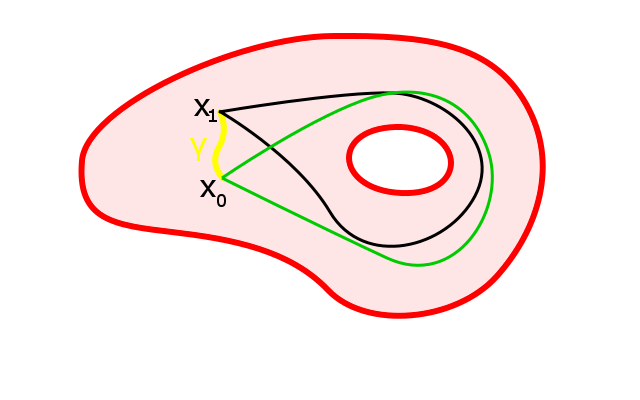
\includegraphics[scale=0.3]{fig65_1.png}} \makebox{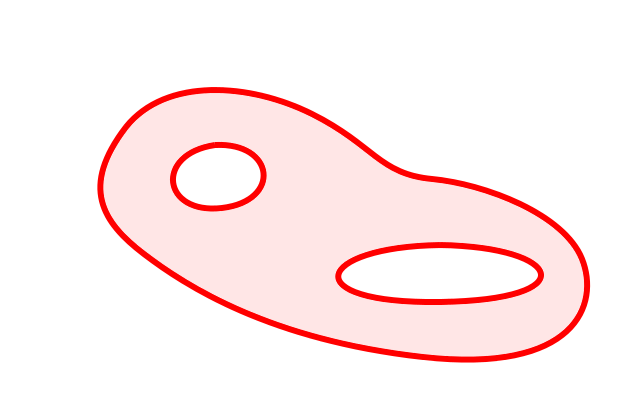
\includegraphics[scale=0.3]{fig65_2.png}}
\caption{}
\end{figure}

Seien nun $x_0,x_1 \in X$ und sei $\gamma$ ein Weg zwischen $x_0$ und $x_1$.
\begin{figure}[ht]
\centering
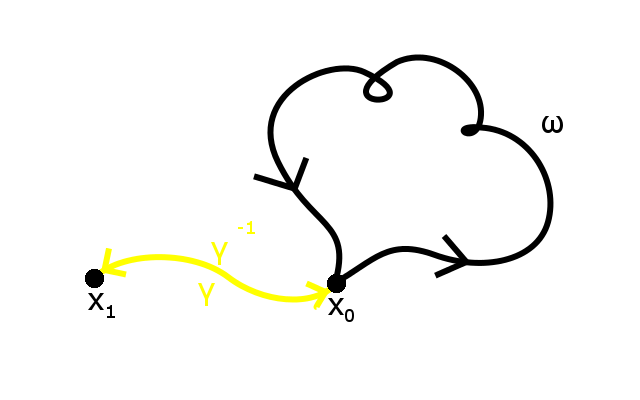
\includegraphics[scale=0.3]{fig66.png}
\caption{}
\end{figure}
Wir definieren eine Abbildung $\tilde \Gamma_\gamma: \Omega(X;x_0)\to \Omega(X;x_1): \omega\mapsto (\gamma*\omega)*\gamma^{-1}$

\begin{st}
 $\tilde \Gamma_\gamma$ induziert einen Isomorphismus:
\[
 \Gamma_\gamma: \pi_1(X;x_0)\to \pi_1(X;x_1): [\omega] \mapsto [\tilde \Gamma_{\gamma}(\omega)]
\]
\end{st}
\begin{proof}
 Zunächst ist die Wohldefiniertheit der Abbildung $\Gamma_\gamma$ zu zeigen, dass heißt zu zeigen ist, dass $\Gamma_{\gamma} ([\omega])$ tatsächlich nur von der Äquivalenzklasse $[\omega]$ und nicht von der Wahl von $\omega$ selbst abhängt, aber es ist klar, dass, wenn $H(t,s)=\omega_S(t)$ eine Homotopie zwischen $\omega$ und $\omega'$ ist, dann auch:
\[
 (t,s)\mapsto (\gamma*\omega_S)*\gamma^{-1}(x)
\]
eine Homotopie zwischen $\tilde \Gamma_{\gamma}(\omega)$ und $\tilde \Gamma_{\gamma}(\omega')$ ist. 

Um die Homomorphieeigenschaft von $\Gamma_{\gamma}$ nachzuweisen, berechnen wir: 
\begin{align*}
 \Gamma_{\gamma}([\omega])\cdot \Gamma_{\gamma} ([\eta])&=[\tilde \Gamma_{\gamma}(\omega)]\cdot [ \tilde \Gamma_{\gamma}(\eta)]\\
&=[(\gamma*\omega)*\gamma^{-1}]\cdot [(\gamma*\eta)*\gamma^{-1}]=[((\gamma*\omega)*\gamma^{-1})*((\gamma*\eta)*\gamma^{-1})]\\
&\stackrel{(*)}=[(\gamma*(\omega*\eta))*\gamma^{-1}]=[\tilde \Gamma_\gamma (\omega*\eta)]=\Gamma_\gamma([\omega] \cdot [\eta]),
\end{align*}

\begin{figure}[ht]
\centering
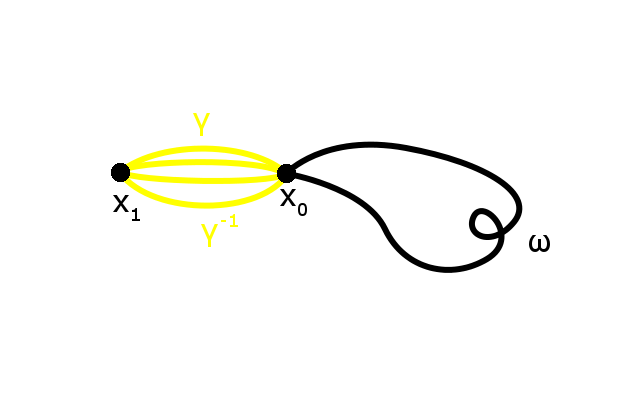
\includegraphics[scale=0.3]{fig67.png}
\caption{}
\end{figure}

wobei wir bei $(*)$ benutzt haben, dass Lemma \ref{thm:2.1.5} sinngemäß auch für Wege gilt. Es gilt, dass $\Gamma_{\gamma^{-1}}$ die Umkehrabbildung von $\Gamma_\gamma$ ist, denn:

\begin{align*}
 \Gamma_{\gamma^{-1}}\circ \Gamma_\gamma ([\omega])&=[(\gamma^{-1}*((\gamma*\omega)*\gamma^{-1}))*\gamma]\\
 &\stackrel{(*)}=[\gamma^{-1}*\gamma]\cdot [\omega]\cdot [\gamma^{-1} * \gamma]=[\omega]
\end{align*}
\end{proof}
\begin{kor}
 Für einen wegzusammenhängenden Raum $X$ hängt die Fundamentalgruppe bis auf Isomorphie nicht von der Wahl des Basispunktes ab.

Deshalb schreibt man bei wegzusammenhängendem $X$ auch oft einfach $\pi_1(X)$ für die Isomorphieklasse der Fundamentalgruppe, zum Beispiel $\pi_1(\R P^n)=\Z_2$ für $n\ge 2$ oder $\pi_1(\R^n)=\{1\}$
\end{kor}
\begin{df}
 Ein topologischer Raum heißt \emph{einfach zusammenhängend}, wenn er wegzusammenhängend ist und eine triviale Fundamentalgruppe hat.

Dann gilt: Jede Schleife ist nullhomotop. Zum Beispiel $\R^n, S^n, n\ge 2$ sind einfach zusammenhängend.  
\end{df}

Um das Verhalten der Fundamentalgruppe und der induzierten Homomorphismen $\pi_1(f)$ unter Homotopie zu untersuchen, führen wir folgende Sprechweise ein: Zwei stetige Abbildungen $f,g: (X;x_0)\to (Y,y_0)$ heißen \emph{punktiert homotop}, wenn es eine Homotopie $H$ von $f$ nach $g$ gibt, so dass für alle $s\in [0,1]$ gilt: $H(x_0, s)=y_0$. Wenn wir ausdrücklich zulassen wollen, dass Homotopien von Abbildungen zwischen punktierte Räumen auch den Basispunkt bewegen dürfen, so sprechen wir von \emph{freier Homotopie}.

\begin{st} \label{thm2:1.16}
 Sind $f,g: (X;x_0)\to (Y;y_0)$ punktiert homotop, so stimmen die induzierten Homomorphismen
\[
 \pi_1(f), \pi_1(g): \pi_1(X;x_0)\to \pi_1(Y;y_0)
\]
überein
\end{st}
\begin{proof}
 Ist $H$ eine Homotopie wie oben, so ist $(t,s)\mapsto H(\omega(t), s)$ eine zwischen $f\circ \omega$ und $g\circ \omega$ mit festen Endpunkten.
\end{proof}

\begin{st}\label{thm2:1.17}
 Sei $H$ eine \emph{freie Homotopie} zwischen den stetigen Abbildungen $f,g: (X;x_0)\to (Y;y_0)$ und sei die Schleife $\delta\in \Omega(Y;y_0)$ durch $\delta(s):=H(x_0, s)$. Dann gilt:
\[
 \pi_1(f)([\omega])=[\delta]\pi_1(g)([\omega]){[\delta]}^{-1}
\]
für jedes $[\omega]\in \pi_1(X;x_0)$.
\end{st}

\begin{proof}
 Dies folgt nach Satz \ref{thm2:1.16}. Man überlegt sich, dass $f\circ \omega$ und $(\delta*(g \circ \omega))*\delta^{-1}$ zueinander homotop mit festen Endpunkten sind. (Übung)
\end{proof}
\begin{kor}
 Sind $f,g$ zueinander inverse Homotopieäquivalenzen, so sind
\[
\pi_1(f):\pi_1(X;x_0)\to \pi_1(Y;y_0)
\]
und
\[
 \pi_1(g):\pi_1(Y;y_0)\to \pi_1(X;x_0)
\]
Isomorphismen der Fundamentalgruppen, die bis auf Konjugation invers zueinander sind. 
\end{kor}
\begin{proof}
 Wende \ref{thm2:1.17} auf $f\circ g \simeq \id_Y, g\circ f \simeq \id_X$ an.  Wobei $\simeq$ die freie Homotopie kennzeichnet.
\end{proof}
\subsection{Überlagerungen}
\begin{df}
 Eine surjektive stetige Abbildung $p: E\to B$ heißt \emph{Überlagerung}, wenn es zu jedem Punkt $x\in B$ eine Umgebung $U$ von $x$ gibt, so dass $p^{-1}(U)$ eine disjunkte Vereinigung von offenen Mengen $V_\alpha,\alpha\in A$ ist und $p|_{V_\alpha}: V_\alpha\to U$ für alle $\alpha\in A$ ein Homöomorphismus ist. In diesem Fall heißt $U\subset B$ \emph{trivial überlagert}, $E_x:=p^{-1}(\{x\})$ heißt \emph{Faser} über $x$.

\begin{figure}[ht]
\centering
\makebox{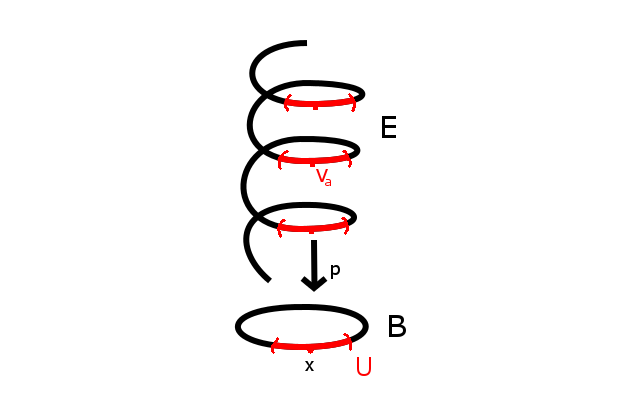
\includegraphics[scale=0.3]{fig68.png}}
\makebox{\fixme[fig69]}
\caption{}
\end{figure}
\setcounter{figure}{69} %%% entfernen, wenn alle weg waren


\end{df}

\begin{exs*}
 \begin{enumerate}[(i)]
  \item $P: \R\to S^1, t\mapsto e^{2\pi it}$ ist eine Überlagerung. Jeder Punkt $z\in S^1$ besitzt zum Beispiel die trivial überlagerte offene Umgebung $S^1\setminus\{-z\}$, 
auf dieser lässt sich die Funktion $z\mapsto \frac{\arg{z}}{2\pi}$ stetig definieren. \\
\begin{figure}[H]
\centering
 \fixme[fig70]
\caption{}
\end{figure}
  \item $p:\C\setminus\{0\}\to \C \setminus\{0\}, z \mapsto z^n, n\in \N$ ist eine Überlagerung.
  \item Jeder Homöomorphismus ist eine Überlagerung $f: E\to B$.
  \item Sei $M$ eine topologische Mannigfaltigkeit und $\Gamma$ eine endliche Gruppe von Homöomorphismen, 
die fixpunktfrei auf $M$ operiert. Nach Satz I.\ref{thm:7.4} ist $M/\Gamma$ eine topologische Mannigfaltigeit. Es  gilt aber auch, dass die Quotientenabbildung $q:M \to M/\Gamma$ eine Überlagerung ist. Denn nach Satz I.\ref{thm:7.4}
ist $q$ ein lokaler Homöomorphismus und im Beweis von Satz I.\ref{thm:7.4} wurde gezeigt, dass es um jeden Punkt $x\in M$ eine Umgebung $U$ gibt, die keine zu $x$ äquivalenten Punkte enthält. Dies zeigt, dass $q(U)$ trivial überlagert wird (von $\Gamma U$).
  \item Spezialfälle von $4$: zum Beispiel $q: S^n\to \R P^n, x \mapsto \{x, -x\}$ ist eine Überlagerung.\\
\begin{figure}[H]
\centering
 \fixme[fig71]
\caption{}
\end{figure}
 \end{enumerate}
\end{exs*}
\fixme[Nummerierung und Ordnung überdenken]\\
\begin{df}
 Sei $p: E\to B$ eine Überlagerung und $f:X\to B$ eine stetige Abbildung.  Eine \emph{Hochhebung} (oder \emph{Lift}) von $f$ ist eine stetige Abbildung $F: X \to E,$ so dass $p\circ F=f$. Mit anderen Worten, eine Hochhebung von $f$ ist eine Abbildung $F$, die das nebenstehende Diagramm kommutativ macht.\\
\begin{center}
\makebox{
\begin{xy}
 (0,0)*+{X}; (40,0)*+{B}; (40, 20)*+{E};
{\ar (2,2)*+{}; (38,20)*+{}}?*!/_2mm/{F};
{\ar (40,18)*+{}; (40,2)*+{} }?*!/_2mm/{p};
{\ar (2,0)*+{}; (38,0)*+{}}?*!/^2mm/{ f};
\end{xy} }
\end{center}

\end{df}
zum Beispiel ist die Abbildung $F:[0,1]\to \R, t\mapsto  5 \cdot t$ eine Hochhebung von $f: [0,1]\to S^1, t \to e^{10\pi t i}$

\begin{figure}[H]
\centering
 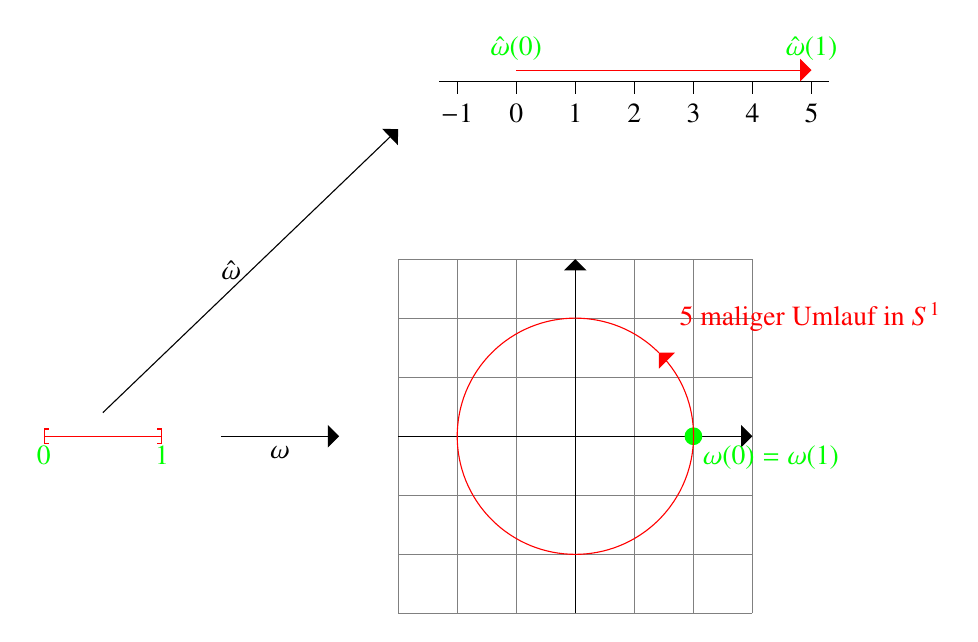
\begin{tikzpicture}[scale=1.5, >=triangle 90]
\begin {scope} [red]
  \draw [[-{]}] (0,0) -- (1,0);
  \draw [green] (0,0) node [anchor=north] {$0$};
  \draw [green] (1,0) node [anchor=north] {$1$};
\end {scope}
\draw [->] (0.5,0.2) -- (3,2.6) node [midway,anchor=east] {$\hat{\omega}$};
\draw [->] (1.5,0) -- (2.5,0) node [midway,anchor=north] {$\omega$};
\begin {scope} [xshift=4cm,yshift=3cm, scale =0.5]
  \draw[step=1cm] (-1.3,-0.2) grid (5.3,0);
  \draw (-1,-0.2) node [anchor=north] {$-1$};
  \draw (0,-0.2) node [anchor=north] {$0$};
  \draw (1,-0.2) node [anchor=north] {$1$};
  \draw (2,-0.2) node [anchor=north] {$2$};
  \draw (3,-0.2) node [anchor=north] {$3$};
  \draw (4,-0.2) node [anchor=north] {$4$};
  \draw (5,-0.2) node [anchor=north] {$5$};
  \draw [red,->](0,0.2) -- (5,0.2);
  \draw [green] (0,0.2) node [anchor=south] {$\hat{\omega} (0)$};
  \draw [green] (5,0.2) node [anchor=south] {$\hat{\omega} (1)$};
\end {scope}
\begin{scope} [xshift=4.5cm,]
\draw[step=.5cm,gray,very thin] (-1.5,-1.5) grid (1.5,1.5);
\draw [->] (-1.5,0) -- (1.5,0);
\draw [->] (0,-1.5) -- (0,1.5); 
\filldraw [green] (1,0) circle (2pt);
\draw [red,->,rotate=45] (1.0cm,0cm) arc (0:360:1.0cm);
\draw [green] (1,0) node [anchor = north west]{$\omega (0) = \omega (1)$};
\draw [red] (0.8,0.8) node [anchor=south west] {5 maliger Umlauf in $S^1$};
\end {scope}
\end{tikzpicture}
\caption{}
\end{figure}

denn $p\circ F(t)=e^{2\pi i F(t)}=e^{2\pi i 5 t}=f(t)$ . Die Hochhebung ist \emph{nicht} eindeutig, denn zum Beispiel ist
$t\mapsto 5t+k, k\in \Z$  ebenfalls eine Hochhebung.
\begin{st}[Eindeutigkeit des Lifts]\label{thm2:2.3}
Sei $p: E \to B$ eine Überlagerung und seien $F,G: X\to E$ zwei Hochhebungen von $f:X\to B$. Sei $X$ zusammenhängend. Wenn es ein $x_0 \in X$ gibt mit $F(x_0)=G(x_0),$ so gilt $F=G$. 
\end{st}
\begin{proof}
 Wir betrachten die beiden Teilmengen
\[
 V:=\{x\in X|F(x) = G(x)\} \text{ und } W:=\{x\in X|F(x)\neq G(x)\}
\]
von $X$ und zeigen, dass beide offen sind, denn dann folgt die Behauptung aus dem Zusammenhang von $X$ und der Tatsache, dass $V$ nicht leer ist (wegen $x_0\in V$). Sei nun $x\in X$ und $U$ eine offene, triviale überlagerte Umgebung von $f(x)\in B$, also
\[
 p^{-1}(U)=\dotcup_{\alpha\in A} V_\alpha
\]
mit $V_\alpha$ offen und homöomorph zu $U$. Sei $F(x)\in V_{\alpha_1}$ und $G(x)\in V_{\alpha_2}$. Dann ist:
\[
 D:=F^{-1}(V_{\alpha_1})\cap G^{-1}(V_{\alpha_2})
\]
eine offene Umgebung von $x$. Es gilt $D\subset V$, falls $\alpha_1=\alpha_2$ und $D\subset W$ falls $\alpha_1\neq \alpha_2$.
\end{proof}
\begin{st}[Homotopie-Hochhebungssatz] \label{thm2:2.4}
 Sei $p: E\to B$ eine Überlagerung und seien $F: X \to E$ sowie $H: X\times [0,1] \to B$ stetige Abbildungen mit $H(x,0)=p(F(x))$ für alle $x\in X$. Dann gibt es genau eine Hochhebung $\tilde H$ von $H$ mit $\tilde H(\cdot, 0)=F(\cdot)$.
\end{st}
\begin{proof}
 \begin{enumerate}[(i)]
  \item Die Eindeutigkeit folgt aus Satz \ref{thm2:2.3} (wende den Satz auf $H|_{\{x\}\times[0,1]}$ an)
  \item Zum Beweis der Existenz genügt es, die Hochhebbarkeit lokal zu beweisen, dass heißt es genügt, folgendes zu zeigen:
\setcounter{figure}{72} %%% entfernen wenn alle Figuren hochgeladen...
\begin{figure}[H]
\centering
 \fixme[fig73]
\caption{}
\end{figure}
Zu jedem $x\in X$ gibt es eine Umgebung $U_x$ und eine Hochhebung $H^x$ von $H|_{U_x\times[0,1]}$. Dann stimmen wegen der Eindeutigkeit verschiedene solchen Abbildungen $H^x, H^y$ auf der Schnittmenge ihrer Definitionsbereiche überein und wir erhalten eine auf ganz $X \times[0,1]$ wohldefinierte Hochhebung $\tilde H$
\item Wir beweisen also die lokale Hochhebbarkeit: 

Sei $x\in X$. Zu jedem $t\in[0,1]$ gibt es ein $\epsilon_t>0$ und eine Umgebung $U_{x,t}$ von $x$ in $X$, so dass $H(U_{x,t}, (t-\epsilon_t, t+ \epsilon_t)$ in einer trivial überlagerten Umgebung von $H(x,t)$ enthalten ist.

Wegen der Kompaktheit von $[0,1]$ überdecken endlich viele der $(t-\epsilon_t, t+\epsilon_t)$ bereits $[0,1]$ und es gibt eine Umgebung $U_x$ und eine Zerlegung
\[
 0=t_0<t_1<\dotsb <t_m=1,
\]
so dass $H(U_x\times (t_k, t_{k+1}))$ ganz in eine trivial überlagerten Menge $U(k)$ enthalten ist. Nun können wir induktiv $H^x: U_{x}\times [0,t_k] \to E$ definieren: Ist $H^x$ auf $U_x\times [0,t_k]$ bereits definiert, so definieren wir $H^x$ auf $U_x\times[t_k,t_{k+1}]$ durch $U_x\times [t_k, t_{k+1}]\stackrel{H}{\to} U(k) \stackrel{(p|V_{\alpha_k})^{-1}}\to V_{\alpha_k}\hookrightarrow E$, wobei $H^x(x,0)=F(x)$ gesetzt wird.
 \end{enumerate}

\end{proof}

Im folgenden wollen wir den Zusammenhang zwischen Fundamentalgruppe und Überlagerung betrachten.
\begin{kor}[Wege-Hochhebungssatz] \label{thm2:2.5}
 Sei $p:E\to B$ eine Überlagerung und $\omega:[0,1]\to B$ ein Weg mit Anfangspunkt $b=\omega(0)$. Dann gibt es zu $e\in E_b=p^{-1}(\{b\})$ genau einen Weg $\tilde \omega: [0,1] \to E$ mit Anfangspunkt $\tilde \omega(0)=e$, der eine Hochhebung von $\omega$ ist.
\end{kor}
Für den Zusammenhang zwischen Fundamentalgruppe und Überlagerungen ist es auch eine wichtige Beobachtung, dass die Endpunkte hochgehobener Wege invariant unter Homotopien (mit festen Endpunkten sind.) 
\begin{kor}[Monodromie Lemma]\label{thm2:2.6}
 Ist $p: E\to B$ eine Überlagerung und sind $ \omega_1, \omega_2: [0,1]\to B$ zwei Wege in $B$ mit Anfangspunkt $b=\omega_1(0)=\omega_2(0)$, 
die zueinander homotop mit festen Endpunkten sind.  Dann haben zwei Lifts $\tilde \omega_1, \tilde \omega_2$ von $\omega_1$ bzw.  $\omega_2$ mit demselben Anfangspunkt $e=\tilde \omega_1(0)= \tilde \omega_2(0)$ auch den selben Endpunkt $\tilde \omega_1(1)=\tilde \omega_2(1)$.
\end{kor}
\begin{proof}
 Sei $H: [0,1] \times [0,1]\to B$ eine Homotopie mit festen Endpunkten und $H(\cdot, 0)=\omega_1, H(\cdot, 1)=\omega_2 $. Nach Satz \ref{thm2:2.4} gibt es genau eine Hochhebung $\tilde H$ von $H$ mit $\tilde H(\cdot, 0)=\tilde \omega_1(\cdot)$, wenn $\tilde \omega_1$ eine Hochhebung von $\omega_1$ ist. 
Nach Korollar \ref{thm2:2.5} ist $\tilde \omega_1$ aber durch $\tilde \omega_1(0)=e$ eindeutig festgelegt.

Sei $U\subset B$ eine trivial Überlagerte offene Umgebung von $\omega_2(1)=H(1,t), \forall_{t \in [0,1]}$. Dann ist $c:= \tilde H(1, \cdot): [0,1]\to E$ eine Abbildung, deren Bild ganz in der disjunkten Vereinigung $\dotcup_{\alpha\in A} V_\alpha=p^{-1}(U)$. 
Falls $\tilde H(1,0)\in V_\alpha$, dann folgt auch $\tilde H(1,t) \in V_\alpha$ (für dasselbe $\alpha$), denn sonst erhält man einen Widerspruch zum Zusammenhang von $[0,1]=\dotcup_{\tilde H(1,[0,1])\cap V_\alpha=\emptyset} c^{-1}(V_\alpha)$.
\end{proof}
Anschaulich sagt der Satz aus, dass der Endpunkt der Hochebung kann nicht springen.

Damit können wir einen genaueren Beweis für $\pi_1(S^1)\homo \Z$ geben:
\begin{st}
 $\pi_1(S^1)\homo \Z$
\end{st}
\begin{proof}
 Die Abbildung $p:\R\to S^1, t\mapsto e^{2\pi i t}$ ist eine Überlagerung. Wir betrachten:
\[
 f:\pi_1(S^1; 1)\to \Z: [\omega] \mapsto \tilde \omega (1)
\]
\begin{figure}[H]
\centering
 \fixme[fig74]
\caption{}
\end{figure}
wobei $\tilde \omega$ die nach Korrolar \ref{thm2:2.5} eindeutige festgelegte Hochebung der Schleife $\omega$ mit $\tilde \omega(0)=0$ ist. Nach dem Monodromielemma Korrolar \ref{thm2:2.6} hängt $\tilde \omega(1)$ nur von der Homotopieklasse von $\omega$ (mit festen Endpunkten) ab, also ist $f$ wohldefiniert.
Wir definieren "'Standard-Schleifen"' im $S^1$ wie folgt: Sei $\tilde \omega_k:= [0,1] \to \R, t \mapsto t * k$ für $k \in \Z$ und $w_k:=p\circ \tilde \omega_k$. Offensichtlich ist $\tilde \omega_k$ eine Hochebung von $\omega_k$ und $f([\omega_k])=k$. Dies zeigt die Surjektivität und die Injektivität folgt daraus, dass je zwei Wege mit denselben Anfangs- und Endpunkten in $\R$ (mit festen Endpunkten) zueinander homotop sind. Um die Homomorphieeigenschaften nachzuweisen überlegt man sich:
\[
 f([\omega_k][\omega_l])=f([\omega_k * \omega_l])=f([\omega_{k+l}])
\]
\end{proof}
\subsection{Gruppenwirkungen und Klassifikation von Überlagerung}
\begin{df}
 Eine Gruppe $G$ zusammen mit einer Topologie heißt \emph{topologische Gruppe}, wenn die \emph{Gruppenoperationen} \emph{Multiplikation} $G\times G \to (a,b)\mapsto ab$ und \emph{Inversenbildung}
$G\to G, g\mapsto g^{-1}$ stetig sind.
\end{df}
\begin{exs*}
 \begin{enumerate}[1)]
  \item Jede abstrakte Gruppe mit der diskreten Topologie ist eine topologische Gruppe.
  \item Untergruppen der $GL(n, \R)$ mit der von $\R^{n^2}$ induzierten Teilraumtopologie.  
  \item Liegruppen sind topologische Gruppen.
 \end{enumerate}
\end{exs*}
\begin{df}\label{thm2:3.2}
 Sei $G$ eine topologische Gruppe und $X$ ein topologischer Raum. Eine(\emph{Gruppen-})\emph{Wirkung} (auch: \emph{Operation}) von $G$ auf $X$ ist eine stetige Abbildung:
\[
 G\times X\to X: (g,x) \mapsto g\cdot x
\]
mit den Eigenschaften $1\cdot x = x, (ab)\cdot x=a\cdot (b\cdot x)$
\end{df}
\begin{note*}
 Stets gilt, dass $x\mapsto g\cdot x$ für ein festes Gruppenelement $g$ ein Homöomorphismus von $X$ ist. denn $g^{-1} \cdot (g\cdot x)=(g^{-1}g)\cdot x=1\cdot x=x.$
\end{note*}
\begin{exs*}
 \begin{enumerate}[1)]
  \item Linkstranslation von $G$ auf sich $g\cdot x:=gx$ für $g,x\in G$.
  \item Rechtstranslation von $G$ auf sich $g\cdot x:=xg^{-1}$
  \item Konjugation: $g \cdot x := gxg^{-1}$
  \item Eine \emph{Darstellung} einer topologischen Gruppe, zum Beispiel die Wirkung von $GL(n, \R)$ auf $\R^n$ durch $A \cdot v := Av$
 \end{enumerate}
\end{exs*}
Wir werden zunächst nur Wirkungen diskreter Gruppen betrachten.

\begin{seg}{Zusammenfassung}
 \begin{description}
  \item[topologische Gruppe:] $(a,b)\mapsto a\cdot b$ und $a\mapsto a^{-1}$ stetig.
  \item[Gruppenwirkung:] einer topologische Gruppe
\[
 G\times X\to X, (g,x) \mapsto g\cdot x=g(x) 
\]
\begin{itemize}
 \item stetig
 \item es gilt $g\cdot (h\cdot x)=(gh)\cdot x$ und $1\cdot x = x$

Automatisch folgt, dass die Abbildung $x\mapsto g\cdot x$ ein Homöomorphismus ist, denn $g^{-1} \cdot (g\cdot x)=(g^{-1}g)\cdot x=1\cdot x=x.$

Zum Beispiel eine Menge von Homöomorphismen von $X$, die abgeschlossen unter der Verkettung ist, zu jedem Homöomorphismus auch das Inverse und die Identität enthält, bildet eine Gruppe zusammen mit einer Wirkung auf $X$ ($g\cdot x:=g(x)$)
\end{itemize}
 \end{description}
\end{seg}
Diese Definition beschreibt genau genommen eine \emph{Wirkung von links}, bei einer \emph{Wirkung von rechts} benutze das Gesetz $g\cdot (h\cdot x)=(hg)\cdot x$ (anstatt $g\cdot(h\cdot x)=(gh)\cdot x$.)

[Wirkungen von rechts werden auch durch $(g,x)\mapsto x\cdot g$ beschreiben, dann haben wir $(x\cdot h)\cdot g=x\cdot (hg)$]

\begin{exs*}[$G=X$]
 durch $g\cdot x:= gx$ ist eine Wirkung, denn es gilt $h\cdot (g\cdot x)=hgx$. Entsprechend ist $g\cdot x=xg$ eine Wirkung von rechts, denn:
\[
 h\cdot(g\cdot x)=h\cdot (xg)=(xg)h=x(gh)=(gh)\cdot x
\]

\[
 g\cdot x=g^{-1}x
\]
ist Wirkung von rechts.
\[
 h\cdot (g\cdot x)=h\cdot(g^{-1}x)=h^{-1}g^{-1}x=(gh)^{-1}x=(gh)\cdot x
\]
\[
 g\cdot x=xg^{-1}
\]
ist Wirkung von links.
\[
 h\cdot(g\cdot x)=h\cdot(xg^{-1})=xg^{-1}h^{-1}=x(hg)^{-1}=(hg)\cdot x
\]
\end{exs*}
\begin{df}\label{thm2:3.3}
 Für eine Gruppenwirkung von $G$ auf $X$ heißt $G\cdot x:=G(x):=\{g\cdot x|g\in G\}$ die \emph{Bahn} oder der Orbit von $x$ und
\[
 G_x=\{g\in G|g\cdot x = x\}
\]
heißt die \emph{Standgruppe} von $x$ oder die \emph{Isotopie(unter)gruppe} von $x$ auch \emph{Stabilisator von $x$}.
\end{df}
\begin{note*}
 $G_x$ ist eine Untergruppe von $G$, denn: $1\cdot x=x$, also $1\in G_x$ seien $g,h \in G_x$, dann gilt $(gh)\cdot x=g\cdot(h\cdot x)=g \cdot x=x$, also $gh\in G_x$ und sei $g\in G_x$, dann gilt $g^{-1} \cdot x=g^{-1}\cdot (g\cdot x)=(g^{-1}g)\cdot x=1x=x$, also auch $g^{-1}\in G_x$.
\end{note*}
\begin{seg}{Zusatz zur Definition:}
 Man sagt eine Gruppenwirkung ist \emph{transitiv}, falls $G\cdot x= X$ für ein $x\in X$.
\end{seg}
\begin{ex*}
 \item $\text{Gl}(n, \R)$ operiert auf $\R^n$ durch $A\cdot x:= Ax\in \R^n$. ($Ex=x, (AB)x=A(Bx)$ Matrixmultiplikation ist assoziativ). Diese Wirkung hat zwei Bahnen nämlich $\{0\}$ und $\R^n\setminus\{0\}$
 \item $\text{Gl}(n, \R)$ operiert auf $\R^{n^2}$ durch $A\cdot X=AXA^{-1}$ entspricht der Basistranformation.
 \item $O(n)$ operiert auf $S^{n-1}=\{x\in \R^n|\,||x||=1\}$ diese Wirkung ist transitiv und
\[
 O(n)_{e_1}=\left \{ \left ( \, \begin{matrix} 1 & \vline & \begin{matrix} 0 & \cdots & 0 \end{matrix}\\ \hline \begin{matrix} 0 \\ \vdots \\ 0\end{matrix}& \vline & \text{\LARGE{A}} \end{matrix}\, \right ) \, | A \in O(n-1)\right \}
\] 
\end{ex*}
\begin{df}\label{thm2:3.4}
 Eine Gruppenwirkung heißt \emph{blätternd}, wenn es zu jedem $x\in X$ eine Umgebung $U$ gibt mit $U\cap g\cdot U=\emptyset$ für alle $g\in G\setminus\{1\}$
\begin{figure}[H]
\centering
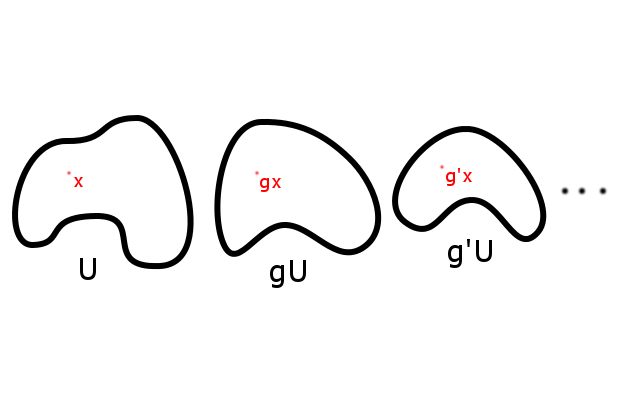
\includegraphics[scale=0.3]{fig75.png} 
\caption{}
\end{figure}
\end{df}


\begin{lem}\label{thm2:3.5}
 Die diskrete Gruppe $G$ wirke blätternd auf den topologischen Raum $X$. Dann ist die Abbildung $\pi: X\to X/G$ eine Überlagerung, wobei $X/G$ den Quotientenraum von $X$ bezüglich der Relation
\[
 x\sim y :\iff x\in G\cdot y \iff \exists g\in G: g\cdot y=x
\]
bezeichnet. ($X/G=\{G\cdot x|x\in X\}$ wird als \emph{Bahnenraum} der Wirkung bezeichnet) eine Überlagerung.


\end{lem}
\begin{proof}
\begin{figure}[H]
\centering
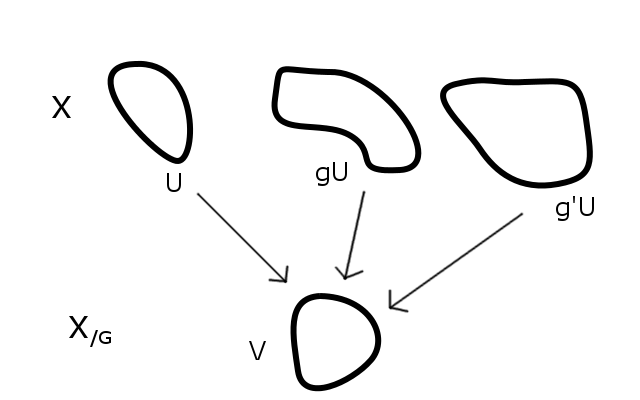
\includegraphics[scale=0.3]{fig76.png} 
\caption{}
\end{figure}
 Sei $[x]=G\cdot x\in X/G$. Sei $U$ eine Umgebung wie in Definition \ref{thm2:3.4} und sei $V:=\pi(U)$, Dann ist $\pi^{-1}(V)=\bigcup_{g\in G} gU$ eine disjunkte Vereinigung, denn falls $g\neq g'$, folgt $g\cdot U \cap g'\cdot U=g\cdot (U\cap(g^{-1}g') \cdot U =g\cdot(\emptyset)=\emptyset$.

Betrachte nun $\pi|_{g\cdot U}$ für ein $g\in G$, $\pi$ ist stetig, wegen "`blätternd"' ist $\pi|_{g\cdot U}$ injektiv und es gilt $\pi(gU)=V$.
Da die Quotientenabbildung offen ist, folgt, dass  $\pi|_{g\cdot U}$ ein Homöomorphismus ist.
\end{proof}
\begin{figure}[H]
\centering
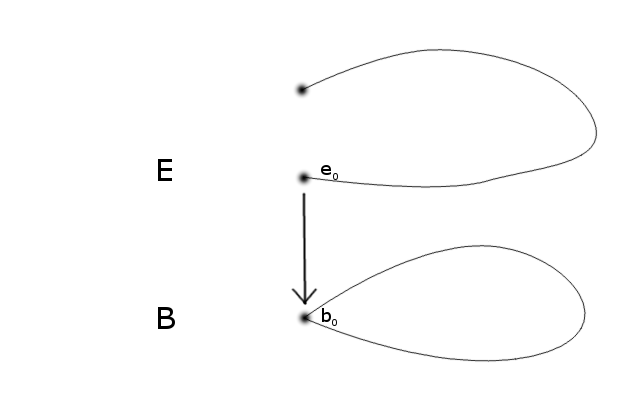
\includegraphics[scale=0.3]{fig77.png} 
\caption{}
\end{figure}
Von nun an bezeichne $p: E \to B$ stets eine Überlagerung und sei $e_0 \in E$ und $b_0=p(e_0)$.
Wir wollen eine Wirkung der Fundamentalgruppe $\pi_1(B; b_0)$ auf der Faser $E_{b_0}$ definieren.\\

\begin{df}
 Sei $\omega:[0,1]\to B$ ein Weg mit Anfangspunkt $b_0=\omega(0)$ und Endpunkt $b_1=\omega(1)$. Es sei
\[
 \tilde \Lambda_\omega: E_{b_0} \times [0,1] \to E
\]
die nach Korollar \ref{thm2:2.5} eindeutig bestimmte Abbildung mit
\[
 p(\tilde \Lambda_\omega (e,t))=\omega(t) \qquad \tilde \Lambda_{\omega}(e,0)=e
\]
Weiter sei $\Lambda_\omega(e):= \tilde \Lambda_\omega(e,1)$
\end{df}
\begin{lem}\label{thm2:3.7}
 Es gilt
\begin{enumerate}[(i)]
 \item $\Lambda_\omega$ bildet $E_{b_0}$ nach $E_{b_1}$ nach.
 \item $\Lambda_{\omega*\eta}=\Lambda_{\eta} \circ \Lambda_\omega$
 \item Sind $\omega$ und $\eta$ homotop mit festen Endpunkten, dann gilt $\Lambda_\omega=\Lambda_\eta$
 \item $\Lambda_\omega: E_{b_0} \to E_{b_1}$ ist bijektiv
\end{enumerate}
\end{lem}
\begin{proof}
 (i) und (ii)  folgen direkt aus der Definition von $\Lambda_\omega$. (iii) folgt aus dem Monodromielemma Korollar \ref{thm2:2.6} (iv) folgt aus (i)-(iii), da $\Lambda_{\omega^{-1}}\circ \Lambda_\omega\stackrel{(ii)}{=} \Lambda_{\omega*\omega^{-1}}=\Lambda_\epsilon=\id_{E_{b_0}}$, wobei $\epsilon$ ein konstanter Weg in $b_0$ ist. 
\end{proof}

\begin{seg}{Zusamenfassung: Überlagerung und Gruppenwirkung}
\begin{figure}[H]
\centering
 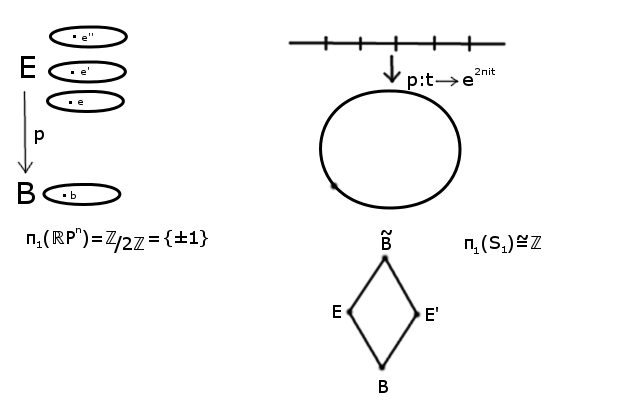
\includegraphics[scale=0.5]{fig78.png}
 \caption{}
\end{figure}
Es ist $\pi_1(\R P^n)=\Z/2\Z=\{\pm 1\}$. (fixen)

Die Fundamentalgruppe wirkt auf der Faser $E_{b_0}$ über $B_0$\\
\begin{figure}[H]
\centering
 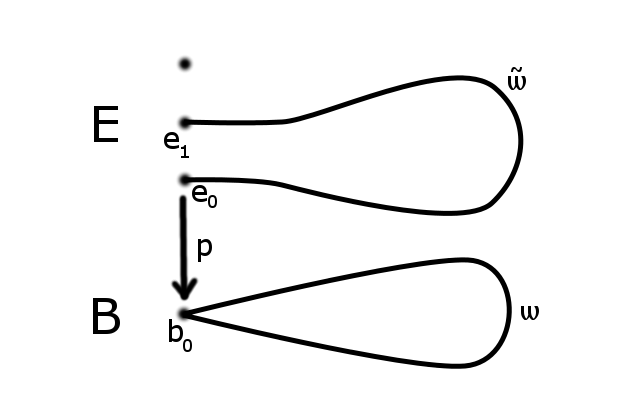
\includegraphics[scale=0.3]{fig79.png}
 \caption{}
\end{figure}


$\Lambda_\omega(e_0)=\tilde \omega(1)$ ist der Endpunkt der Hochhebung $\omega$ mit Startpunkt $e_0$

Wir haben bereits einige Eigenschaften bewiesen:
\begin{enumerate}[(i)]
 \item $\Lambda_\omega: E_{b_0} \to E_{b_1}$
 \item $\Lambda_{\omega*\eta}=\Lambda_{\eta} \circ \Lambda_{\omega}$
 \item $\omega, \eta$ homotop mit festen Endpunkten $\implies \Lambda_\omega=\Lambda_\eta$
 \item $\Lambda_\omega: E_{b_0} \to E_{b_1}$ Bijektion\\
\begin{figure}[H]
\centering
 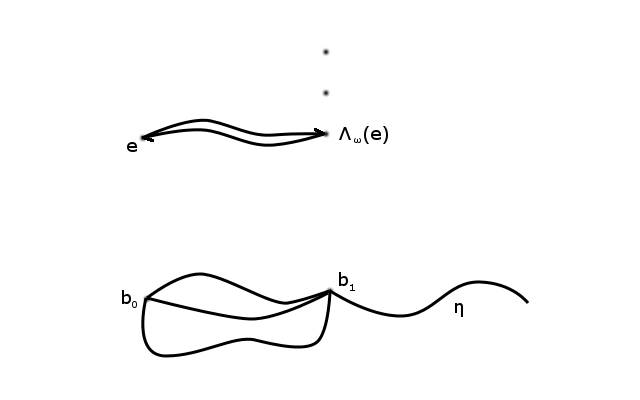
\includegraphics[scale=0.3]{fig80.png}
 \caption{}
\end{figure}
\end{enumerate}
\fixme[from mathematiker : Vielleich sind fixes nötig]
\end{seg}

\begin{st}\label{thm2:3.8}
 Die Fundamentalgruppe $\pi_1(B; b_0)$ operiert von rechts auf der Faser $E_{b_0}=p^{-1}(\{b_0\})$ vermöge:
\[
 e\cdot [\omega] := \Lambda_\omega(e)
\]
Die Standgruppe des Punktes $e_0$ ist dabei die Untergruppe
\[
 H(p;e_0):=\pi_1(p) (\pi_1(E;e_0))\subset \pi_1(B;b_0)
\]
Ist $E$ wegzusammenhängend, so ist die Wirkung transitiv und induziert die Bijektion
\[
 E_{b_0} \leftrightarrow \pi_1(B; b_0) / H(p; e_0)
\]



\end{st}
\begin{note*}
\begin{itemize}
\item $G\cdot x \stackrel{1:1}{\leftrightarrow} G/G_x$ operiert eins zu eins.
\item Sei $G$ eine Gruppe und $H \subset G$ Teilmenge, dann kann man definieren:
\[
 gH:=\{g\cdot h|h \in H\}
\]
natürlich kann man auch definieren:
\[
 Hg:=\{h\cdot g|h\in H\}
\]
Man bezeichnet diese als Links- bzw. Rechtsnebenklasse.

\begin{seg}{Allgemeine Tasache:}
 mit der Gruppenwirkung von $G$ auf $X$:
\[
 G\cdot x \stackrel{\text{bijektiv}}{\longleftrightarrow} G/G_x
\]
\[
 g\cdot x \mapsfrom gG_x
\]
Es ist $gh\cdot x=g\cdot x$ und $gG_x=ghG_x$ mit $h\in G_x$
\end{seg}
\end{itemize}
\end{note*}
\begin{proof}
 Aus Lemma \ref{thm2:3.7}(iii) folgt, dass die Abbildung $([\omega], e)\mapsto \Lambda_\omega(e)$ wohldefiniert ist und dass gilt $(1,e) \mapsto \Lambda_\epsilon(e)=e$. Aus (ii) folgt $(e\cdot [\omega])\cdot [\eta]=\Lambda_{\eta}(\Lambda_\omega(e))=\Lambda_{\eta}\circ \Lambda_{\omega}(e)=\Lambda_{\omega*\eta}(e)=(e\cdot [\omega*\eta])=e\cdot ([\omega][\eta])$. Dies zeigt den ersten Teil der Behauptung. Die Standgruppe von $e_0$ besteht aus den Homotopieklassen von Schleifen, die sich zu geschlossenen Wegen mit Anfangs- und Endpunkt $e_0$ hochheben, also aus dem homomorphen Bild von $\pi_1(E; e_0)$ unter $\pi_1(p)$. Falls $E$ wegzusammenhängend ist, gibt es zu je zwei Punkten $e_0, e_1 \in E_{b_0}$ einen verbindenden Weg $\eta$ in $E$. Dann ist $\omega:= p \circ \eta$ eine Schleife in $B$ mit Anfangs- und Endpunkt $b_0$ und es gilt $\Lambda_{\omega}(e_0)=e_1$
\end{proof}
\begin{kor}\label{thm2:3.9}
 $\pi_1(p): \pi_1(E; e_0)\to \pi_1(B, b_0)$ ist injektiv
\end{kor}
\begin{proof}
 Folgt aus dem Homotopie-Hochhebungssatz \ref{thm2:2.4}. Ist das Bild einer Schleife homotop mit festen Endpunkten zu einer konstanten Schleife, so auch die Hochhebung.
\end{proof}
\begin{df}
 Ein topologischer Raum $X$ heißt \emph{lokal wegzusammenhängend}, wenn es zu jedem Punkt $x\in X$ und jeder Umgebung $U$ von $x$ eine wegzusammenhängende Umgebung von $x$ gibt, die in $U$ enthalten ist. 
\end{df}
\begin{note*}
Um ein Gegenbeispiel zu finden, sollten wir eine Menge finden, die gerade so ist, dass eine Wegstück außerhalb zu finden ist, also in etwa so:
\begin{figure}[H]
\centering
 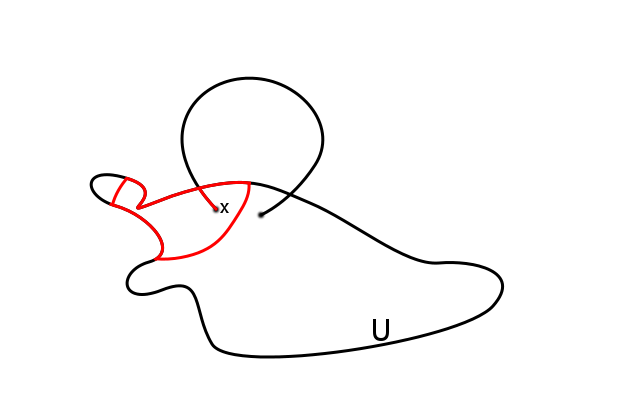
\includegraphics[scale=0.3]{fig81.png}
 \caption{}
\end{figure}
 wegzusammenhängend $\centernot \implies$  lokal wegzusammenhängend.  Gegenbeispiel: Vereinigung von Geradenstücken in $\R^2$:\\
\begin{figure}[H]
\centering
 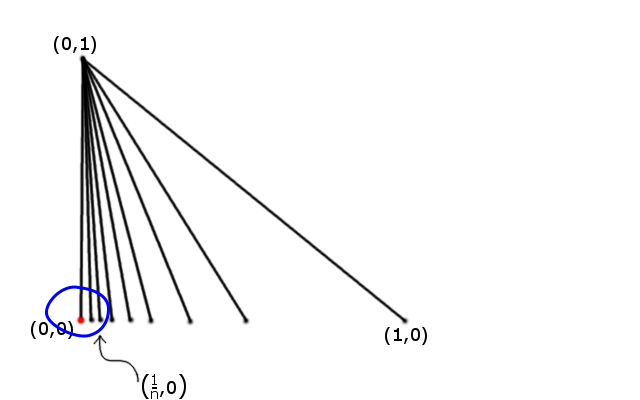
\includegraphics[scale=0.3]{fig82.png}
 \caption{}
\end{figure}

 wegzusammenhängend $\nimplies$ lokal wegzusammenhängend. Gegenbeispiel: Zweipunktmenge.
\end{note*}
\begin{st}[Hochhebungssatz] \label{thm2:3.11}
 Sei $X$ ein sowohl wegzusammenhängender als auch lokal wegzusammenhängender topologischer Raum, $f:X \to B$ eine stetige Abbildung mit $f(x_0)=b_0$. Dann besitzt $f$ genau dann eine Hochhebung $F: X\to E$ (dass heißt $p\circ F=f$) mit $F(x_0)=e_0$, wenn gilt:
\[
 \underbrace{\pi_1(f) (\pi_1(X;x_0))}_{\text{Bild von $\pi_1(f)$}} \subset \underbrace{\pi_1(p) (\pi_1(E;e_0))}_{\text{Bild von $\pi_1(p)$}}
\]
Es sei angemerkt, dass $\pi_1(p) (\pi_1(E;e_0))\subset \pi_1(B; b_0)$ 
\end{st}

\begin{note*}
 $f:X\to Y, f(x_0)=y_0$ induziert  $\pi_1(f):\pi_1(X;x_0)\to \pi_1(Y;y_0): [\omega]\mapsto [f\circ \omega]$\\
\begin{figure}[H]
\centering
 \makebox{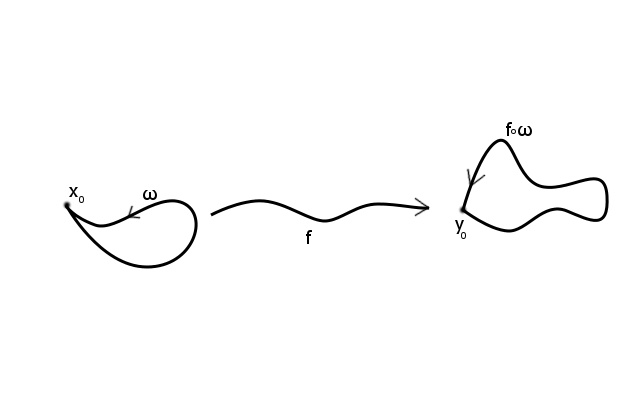
\includegraphics[scale=0.3]{fig83.png}}
 \makebox{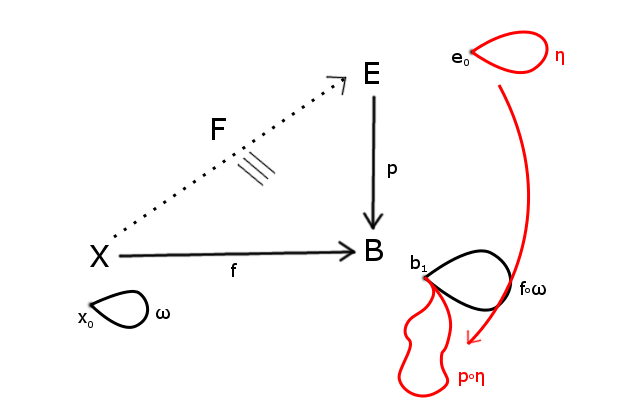
\includegraphics[scale=0.3]{fig84.png}}
 \caption{}
\end{figure}
\setcounter{figure}{84} %%% entfernen wenn alle Grafiken hochgeladen sind
\end{note*}
\begin{proof}
 Wegen $p\circ F=f$ ist klar, dass die Bedingung erfüllt ist, wenn die Hochhebung $F$ existiert. (Denn: $\im(\pi_1(f))=\im(\pi_1(p\circ f))=\im(\pi_1(p)\circ \pi_1(F))\subset \im(\pi_1(p))$). Angenommen, die Bedingung sei erfüllt. Sei $x\in X$. Wir wählen einen Weg $\omega$ von $x_0$ nach $x$ und definieren $F(x):= \Lambda_{f\circ \omega}(e_0)$, denn wenn $F$ existiert, muss es dieser Gleichung genügen. 
\begin{figure}[H]
\centering
 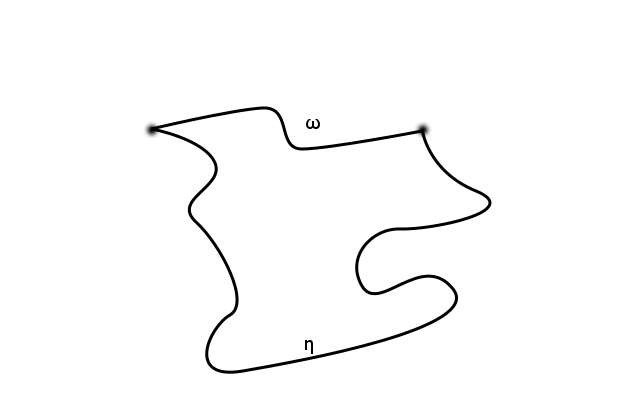
\includegraphics[scale=0.3]{fig85.png}
 \caption{}
\end{figure}
Wir zeigen, dass $F$ wohldefiniert ist. Sei $\eta$ ein weiterer Weg von $x_0$ nach $x$. Dann ist $\Lambda_{f\circ \omega}(e_0)=\Lambda_{f\circ \eta} (e_0)$, falls sich $f\circ(\omega*\eta^{-1})$ zu einem geschlossenen Weg mit Anfangs- und Endpunkt $e_0$ hocheben. Dies gilt aber genau dann, wenn $f\circ(\omega*\eta^{-1})$ das Bild einer geschlossenen Schleife in $E$ mit Anfangs- und Endpunt $e_0$ ist, was durch die Bedingung garantiert ist.

Die Stetigkeit von $F$ folgt aus dem lokalen Wegzusammenhang. Der lokale Wegzusammenhang von $X$ garantiert die Stetigkeit von $F$, denn es gibt um jeden Punkt $x\in X$ eine wegzusammenhängende Umgebung, die unter $f$ in eine schlicht überlagerte Umgebung von $f(x)$ in $B$ abgebildet wird. 
\end{proof}

\begin{note*}[Hochhebungssatz anschaulich]
Erinnerung: die induzierten Homomorphismen auf den Fundamentalgruppen sind:
\[
 f: X\stackrel{\text{stetig}}{\longrightarrow} Y: x_0\mapsto y_0
\]
induziert:
\[
 \pi_1(X;x_0) \stackrel{\pi_1(f)}{\longrightarrow} \pi_1(Y;y_0): [\omega] \mapsto [f\circ w]
\]
\begin{figure}[H]
\centering
 \fixme[fig86]
\caption{}
\end{figure}
Eine Hochhebung sieht folgendermaßen aus:
\begin{figure}[H]
\centering
 \fixme[fig87]
\caption{}
\end{figure}
\begin{seg}{Idee:}
 Wege können hochgehoben werden. Finde Weg von $x_0$ nach $x$ und setze $F(x):=\tilde \omega(1)$, wobei $\tilde \omega$ Hochhebung von $\omega$.
\end{seg}

\begin{seg}{Problem:}
 Es kann verschiedene Wege von $x_0$ nach $x$ geben, zum Beispiel:\\
\begin{figure}[H]
\centering
 \fixme[fig88]
\caption{}
\end{figure}
Zwei Wege von $x_0$ nach $x$ entspricht einer Schleife von $x_0$ durch $x$. Es muss also eine Schleife $\phi$ in $E$ geben, so dass $[f\circ \omega*\eta^{-1}]=[p\circ \phi]$, dass heißt es muss $\im(\pi_1(f))\subset \im(\pi_1(p))$.
\begin{figure}[H]
\centering
 \fixme[fig89]
\caption{}
\end{figure}
\end{seg}
\end{note*}
Wir wollen Satz \ref{thm2:3.11} verwenden, um zwei verschiedene Überlagerungen über demselben \emph{Basisraum} $B$ zu vergleichen. Wir wollen also folgende Situation betrachten:
\begin{figure}[H]
\centering
 \begin{tikzpicture}[description/.style={fill=white,inner sep=2pt}]   
\matrix (m) [matrix of math nodes, row sep=3em,
    column sep=2.5em, text height=1.5ex, text depth=0.25ex]
    { E & & E' &&E\\
      &&&&E'\\
      B  & &B &&B\\ };
    %\draw[double,double distance=5pt] (m-1-1) – (m-1-3);
       \path[->,font=\scriptsize]
    (m-1-1)  edge node[auto] {$ f $} (m-1-3)
     (m-1-1) edge node[auto,swap] {$ p $} (m-3-1)
    (m-3-1) edge node[auto,swap] {$ id_B $} (m-3-3)
    (m-1-3) edge node[auto] {$ p' $} (m-3-3)
    (m-1-5) edge node[auto] {$ f $} (m-2-5)
    (m-2-5) edge node[auto] {$ p' $} (m-3-5);
\end{tikzpicture}


\caption{}
\end{figure}
Wir wollen die Frage studieren, wann sich die Abbildung $\id_B\circ p:E\to B$ zu einer Abbildung $f:E \to E'$ hochheben lässt. Damit wir den Hochhebungssatz anwenden können, nehmen wir an, dass $B$ wegzusammenhängend und lokal wegzusammenhängend ist. 
\begin{kor}\label{thm2:3.12}
 Sei $B$ wegzusammenhängend und lokal wegzusammenhängend. Seien $p:E\to B$ und $p':E'\to B$ Überlagerung mit wegzusammenhängenden \emph{Totalräumen} $E$ und $E'$.

Es seien $e_0\in E, e'_0\in E'$ und $b=p(e_0)=p'(e'_0)$. Dann existiert genau dann eine stetige Abbildung $f:E\to E'$ mit $p'\circ f=p$ und $f(e_0)=e'_0$, wenn gilt $\pi_1(p)(\pi_1(E,e_0))\subset \pi_1(p')(\pi_1(E', e'_0))$ (bzw. $\im(\pi_1(p))\subset \im \pi_1(p')$).
\end{kor}
\begin{note*}
 Den Urbildbereich einer Überlagerung bezeichnet man als \emph{Totalraum}. Und den Bildbereich \emph{Basisraum} $B$. 
\end{note*}
Wie man sich leicht überlegt überlegt, gilt in der Situation von Korollar \ref{thm2:3.12} auch, dass $f:E\to E'$ eine Überlagerung ist. Dies motiviert insbesondere folgende Definition:

\begin{df}
 Eine Überlagerung $p:E\to B$ heißt \emph{universelle Überlagerung}, wenn $E$ einfach zusammenhängend ist (also $\pi_1(E)\cong \{1\}$ ist).
\end{df}
Wir wollen den Hochhebungssatz nun benutzen, um eine Wirkung einer gewissen Untergruppe der Fundamentalgruppe der Basis auf den Totalraum zu definieren. Es handelt sich dabei um die Fortsetzung der in Satz \ref{thm2:3.8} definierten Wirkung auf der Faser $E_b$.

Wir betrachten der Spezialfall $E=E'$ des Korollars. 
\begin{figure}[H]
\centering
 \begin{tikzpicture}[description/.style={fill=white,inner sep=2pt}]   
\matrix (m) [matrix of math nodes, row sep=3em,
    column sep=2.5em, text height=1.5ex, text depth=0.25ex]
    { E & & E\\
      &&\\
      B  & &B\\ };
    %\draw[double,double distance=5pt] (m-1-1) – (m-1-3);
       \path[->,font=\scriptsize]
    (m-1-1)  edge node[auto] {$ f $} (m-1-3)
     (m-1-1) edge node[auto,swap] {$ p $} (m-3-1)
    (m-3-1) edge node[auto,swap] {$ id_B $} (m-3-3)
    (m-1-3) edge node[auto] {$ p $} (m-3-3);
\end{tikzpicture}


%\caption{}
\end{figure}

Ist $\tilde \omega$ ein Weg von  $e_0$ nach $e'_0$ in $E$ und $\omega=p\circ \tilde \omega,$ so gilt
\[
 \pi_1(p)(\pi_1(E;e'_0))=[\omega]^{-1}\cdot \pi_1(p)(\pi_1(E;e_0)\cdot [\omega]
\]

\begin{figure}[H]
\centering
 %\input{fig91}
 \fixme[fig91]
\caption{}
\end{figure}
Genau dann gibt es eine stetige Hochhebung $f:E\to E$ der Identität auf $B$ mit $f(e_0)=e'_0$, wenn die obige Gruppe $\pi_1(p)(\pi_1(E;e_0))$ enthält, mit anderen Worten, wenn diese Untergruppe unter Konjugation mit $[\omega]$ invariant bleibt.

\begin{note*}
Konjugation von $a$ mit $g$ ist $gag^{-1}$
\end{note*}

Wir benutzen den folgenden Begriff aus der Gruppentheorie:

Sei $G$ eine Gruppe und $H$ eine Untergruppe. Man sagt, ein Element $g\in G$ \emph{normalisiert} $H$, falls $gHg^{-1}=H$ gilt. Die Menge 
\[
 N_G(H)=\{g\in G| gHg^{-1}=H\}
\]
aller Elemente, die $H$ normalisieren heißt \emph{Normalisator} von $H$. Falls $N_G(H)=G$, dass heißt falls $gHg^{-1}=H \, \forall g\in G$, dann sagt man, $H$ ist eine \emph{normale Untergruppe}. Für solche gilt, dass die Menge der Nebenklasse $G/H:=\{gH|g\in G\}$ eine natürliche Gruppenstruktur hat $(g\cdot H)\cdot (k\cdot H)=g k \underbrace{(k^{-1}Hk)}_{=H}H=g\cdot k \cdot HH=g\cdot k \cdot H$.

Wie man sich leicht überlegt, ist $N_G(H)\subset G$ eine Untergruppe.  

\begin{st}\label{thm2:3.14}
 Sei $B$ wegzusammenhängend und lokal wegzusammenhängend. Sei $p:E\to B$ eine Überlagerung mit wegzusammenhängendem Totalraum. Es sei \fbox{$H(p;e_0)=\pi_1(p)(\pi_1(E;e_0))$} und sei $N(p;e_0)$ der Normalisator von $H(p;e_0)$ in $\pi_1(B;b_0) $, wobei $b_0=p(e_0)$. 
Dann operiert die diskrete Gruppe $N(p;e_0)/H(p;e_0)$ blätternd von rechts auf $E$, so dass die von den Gruppenelementen induzierten Homöomorphismen Hochhebungen von $p:E\to B$ sind.

Ferner gilt für eine Untergruppe $K$ von $N(p;e_0)$, mit $K\supset H(p,e_0)$, dass
\[
 \bar p: E/K \to B, eK\mapsto p(e) 
\]
 eine Überlagerung ist mit $\pi_1(\bar p)(\pi_1(E/K; e_0 K))=K$.
\begin{figure}[H]
\centering
 \fixme[fig92]
\caption{}
\end{figure}
\end{st}
\begin{note*}
\begin{itemize}
\item Insbesondere gilt, wenn $E$ einfach zusammenhängend ist, also $\pi_1(E;e_0)=\{1\}$, dann folgt $H(p;e_0)\cong \{1\}$ und $N(p;e_0)=\pi_1(B;b_0)$.
\item $H(p;e_0)$ wird auch als \emph{charakteristische Untergruppe} von $p$ genannt.
\end{itemize}
\end{note*}
\begin{proof}
\begin{figure}[H]
\centering
 \fixme[fig93]
\caption{}
\end{figure}
 Zunächst ist klar, dass die oben definierten stetigen Abbildungen $E\to E$ stetige Fortsetzungen der Wirkung der 
Fundamentalgruppe $\pi_1(B;b_0)$ auf der Faser über $b_0$ sind (vgl. Satz \ref{thm2:3.8}) auf ganz $E$ sind.  Diese 
Abbildungen sind also nach dem Hochhebungssatz bereits eindeutig durch das Bild des Puntkes $e_0$ bestimmt. 
Daraus folgt, dass es sich um eine Gruppenwirkung handelt. Die Untergruppe $H(p, e_0)$ ist dabei 
gerade die Standgruppe von $e_0$ diese Elemente wirken trivial auf $E$.

Da die von dieser Gruppenwirkung induzierte Homöomorphismen von $E$ mit $p$ verträglich sind, wirken sie auf dem Urbild $p^{-1}(U)=\dotcup_{\alpha} U_\alpha$ einer trivial überlagerten Umgebung $U$ durch Permutation der Blätter $U_\alpha$, (also ist die Gruppenwirkung blätternd.)
\begin{figure}[H]
\centering
 \fixme[fig94]
\caption{}
\end{figure}
Also ist nach Lemma \ref{thm2:3.5} die Abbildung $\bar{p}$ eine Überlagerung. Die Aussage über das Bild von $\pi_1(\bar p)$ ergibt sich aus Satz \ref{thm2:3.8}, denn $K$ ist die Standgruppe der $\pi_1(B;b_0)$-Wirkung auf der Faser $\bar p^{-1}(b_0)$ in diesem Fall.
\end{proof}
Mit Hilfe von Satz \ref{thm2:3.14} können wir nun \emph{alle} Überlagerungen des Raumes $B$ konstruieren, sobald wir eine universelle (=einfach zusammenhängende) Überlagerung $\tilde p: \tilde B\to B$ gefunden haben, denn für diese gilt $H(\tilde p; e_0)=\{1\}$ und $N(\tilde p; e_0)=\pi_1(B;b_0)$, dass heißt wir können damit zu jeder Untergruppe $K\subset \pi_1(B;b_0)$ eine "'passende"' Überlagerung $p:E\to B$ mit $H(p;e_0)=K$ konstruieren.
Aus Korrolar \ref{thm2:3.12} (Vergleich von Überlagerungen) folgt nämlich insbesondere, dass zwei Überlagerungen $p_1, p_2: E_1, E_2 \to B$ mit $H(p_1;e_0)=H(p_2;e'_0)$ \emph{isomorph} sind, dass heißt es gibt einen Homöomorphismus $f:E_1\to E_2$ mit $p_2\circ f = p_1$.

Die Existenz einer universellen Überlagerung werden wir im nächsten Abschnitt beweisen (unter gewissen Voraussetzungen).

\subsection{Universelle Überlagerung und Decktransformationen}
Zunächst wollen wir eine Anwendung der universellen Überlagerung betrachten. Wir wollen die Gruppe der Decktransformationen einführen, die zur Fundamentalgruppe der Basis isomorph ist. Dies liefert in vielen Fällen eine einfache Möglichkeit, Fundamentalgruppen zu bestimmen.
\begin{df}
 Sei $p:E\to B$ eine Überlagerung. Ein Homöomorphismus $f:E\to E$ heißt \emph{Decktransformation} oder \emph{Automorphismus} der Überlagerung $p$, falls $p \cdot f=p$.
\end{df}
Decktransformationen sind also Homöomorphismen von $E\to E$, die jede einzelne Faser $E_b=p^{-1}(\{b\})$ in sich abbilden. Damit ist klar, dass Inverse und Komposition von Decktransformationen wiederum Decktranformationen sind und die Decktransformationen bilden eine Gruppe $\Deck(p)=\Aut(p)$.
\begin{st}
 Sei $p:E\to B$ eine universelle Überlagerung. Dann gilt $\Deck(p)\cong \pi_1(B)$, falls $B$ wegzusammenhängend und lokal wegzusammenhängend ist.

\begin{figure}[H]
\centering
 \fixme[fig95]
\caption{}
\end{figure}
\end{st}
\begin{seg}{Anwendung}
 zum Beispiel erhalten wir sogleich:
\begin{itemize}
 \item $\pi_1(S^1)\cong \Z$\\
\begin{figure}[H]
\centering
 \fixme[fig96]
\caption{}
\end{figure}
 \item $\pi_1(\R P^1)\cong \Z_2$

\end{itemize}

\end{seg}
\begin{proof}
 Nach Satz \ref{thm2:3.14} gilt bei universellen Überlagerungen, dass die Gruppe $N(p; e_0)/H(p;e_0)=\pi_1(B;b_0)/\{1\}=\pi_1(B;b_0)$ blätternd auf $E$ durch Decktransformationen wirkt. Insbesonders wirkt nur die Identität trivial und wir erhalten einen injektiven Homomorphismus:
\[
 \jota: \pi_1(B;b_0)\to \Deck(p)
\]
Es bleibt die Surjektivität zu zeigen.  Sei also $\gamma\in \Deck(p)$. Sei $\omega$ ein Weg von $e_0$ nach $e_0\cdot \gamma$. Dann ist $p\circ \omega$ eine Schleife mit Basispunkt $b_0$. Dies liefert eine Abbildung $f: \Deck(p)\to \pi_1(B,b_0)$, denn: ist $\eta$ ein zweiter Weg von $e_0$ noch $e_0 \cdot \gamma$,
\begin{figure}[H]
\centering
 \fixme[fig97]
\caption{}
\end{figure}
so ist $\eta$ zu $\omega$ homotop mit festen Endpunkten, wegen des einfachen Zusammenhangs von $E$. Es gilt $\jota\circ f = \id_{\Deck(p)}$, denn der Homöomorphismus $\jota(f(\gamma))$ bildet $e_0$ auf $e_0\cdot \gamma$ ab, und wir schließen daraus, dass $\jota(f(\gamma))=\gamma$, denn sonst gäbe es neben der Identität auf $E$ eine zweite Hochhebung von $p$, nämlich $\iota(f(\gamma))\gamma^{-1}$, die $e_0$ auf sich abbildet, im Widerspruch zu Satz \ref{thm2:2.3}.
\end{proof}
\begin{kor}
 Sei der topologische Raum $X$ einfach zusammenhhängend und lokal wegzusammenhängend. Die diskrete Gurppe $\Gamma$ operiere blätternd auf $X$, dann gilt für die Überlagerung $p: X\to X/\Gamma$, $x\mapsto x \cdot \Gamma$, dass $\Gamma=\Deck(p)\cong\pi_1(X/\Gamma)$.
\end{kor}
\begin{proof}
 Offensichtlich sind die Elemente von $\Gamma$ Decktransformationen von $X$, denn die Bahnen der $\Gamma$-Wirkung sind gerade die Fasern der Überlagerung, also $\Gamma\subset \Deck(p)$. Sei $e\in X$. Es gilt also zu jedem Element der Faser $e'\in E_{p(e)}=e\cdot \Gamma$ ein $\gamma \in \Gamma$ mit $e\cdot \gamma=e'$, da die Decktransformationen durch das Bild eines Punktes eindeutig bestimmt sind, kann es also nicht mehr Elemente in $\Deck(p)$ geben, die nicht in $\Gamma$ liegen. 
\end{proof}
\begin{note*}
 Zum Beispiel: $T^2 = \R^2 / \Z^2 \implies \pi_1(T^2) \simeq \Z \times \Z$
\end{note*}

Im folgenden wollen wir einen Satz über die Existenz der universellen Überlagerung zeigen. Zunächst überlegen wir uns eine notwendige Bedingung.
\begin{df}
 Ein topologischer Raum $B$ heißt \emph{semi-lokal einfach zusammenhängend}, wenn jedes $b\in B$ eine Umgebung $U\subset B$ besitzt, so dass jede Schleife in $U$ mit Basispunkt $b$ in $B$ nullhomotop ist.
\end{df}
\begin{note*}
\item "`lokal einfach zusammenhängend"' wäre: In jeder Umgebung von $b$ gibt es eine einfach zusammenhängende Umgebung von $b$.
\end{note*}
\begin{ex*}["`Hawaiische  Ohrringe"']
Die  Hawaiischen  Ohrringe sind weder lokal einfach zusammenhängend noch semi-lokal einfach zusammenhängend.
 \begin{figure}[H]
\centering
 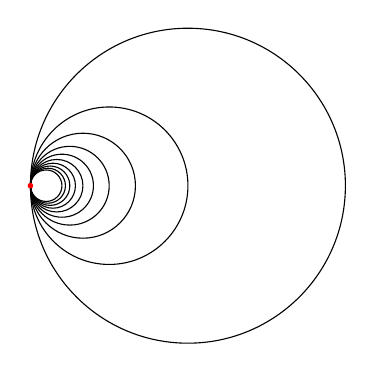
\begin{tikzpicture}[scale=2, >=triangle 90]
\begin{scope}[xshift=2cm]
  \foreach \x in {1,...,10}
     { \draw (1/\x,0) circle (1/\x );
	
      }
\filldraw [red] (0,0) circle (0.4pt);
\end{scope}
\end{tikzpicture}


\caption{}
\end{figure}
\end{ex*}

\begin{ex*}["`Kegel über den Hawaiischen  Ohrringen"']
Beispiel für einen Raum, der semi-lokal einfach zusammenhängend, aber nicht lokal einfach zusammenhängend ist, ist der "`Kegel über den Hawaiischen  Ohrringen"'
\begin{figure}[H]
\centering
 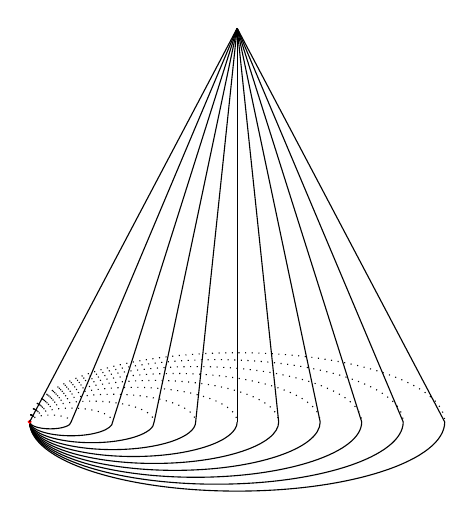
\begin{tikzpicture}[scale=5, >=triangle 90,rotate=90]
\begin{scope}
  \foreach \x in {1,...,10}
     { \draw [dotted] (0 pt,0) arc (90:-90:0.5*\x pt and 1.5*\x pt);
	\draw (0,0) arc (90:270:0.5*\x pt and 1.5*\x pt);
	\draw [-] (0,-3*\x pt) -- (1,-15.pt);
      }
  \filldraw [red] (0,0) circle (0.1pt);
  \draw [-] (0,0pt) -- (1,-15.pt);
\end{scope}
\end{tikzpicture}


\caption{}
\end{figure}
\end{ex*}
\begin{note*}
 Diese Eigenschaft ist notwendig für die Existenz einer universellen Überlagerung $p: E \to B$;
\begin{figure}[H]
\centering
\fixme[fig100]
\caption{}
\end{figure}
Denn sei $U \subset B$ eine trivial überlagerte Umgebung, dann lässt sich jede geschlossene Schleife in $U$ zu einer \emph{geschlossenen} Schleife in $E$ hochheben und dort zusammenziehen. Verketten mit $p$ liefert die Homotopie zur konstanten Schleife in $B$.
\end{note*}

\subsubsection*{Vorbemerkung zur Konstruktion der universellen Überlagerung}
 Um die Idee der Konstruktion besser zu verstehen, wollen wir zunächst annehmen, dass $p:E\to B$ bereits eine universelle Überlagerung ist.

Sei $b_0\in B$ ein fest gewählter Basispunkt und $b_1$ ein weiterer Punkt in $B$, wenn $w$ ein Weg von $b_0$ nach $b_1$ ist, dann erhalten wir mit der in Abschnitt 3 eingeführter Abbildung $\Lambda_\omega$ eine Abbildung von der Faser $E_{b_0}$ in die Faser $E_{b_1}$. Diese hängt nur von der Homotopieklasse (mit festen Endpunkten) ab.\\
\begin{figure}[H]
 \centering
\fixme[fig101]
\caption{}
\end{figure}
Ist andereseits $\Lambda_{\omega}(e)=\Lambda_{\eta}(e)$ für einen anderen Weg $\eta$ von $b_0$ nach $b_1$, dann ist $\eta$ auch homotop (m.f.E.\footnote{mit festen Endpunkten}) zu $\omega$, denn die Hochhebungen von $\omega$ und $\eta$ lassen sich ineinander deformieren, da $E$ einfach zusammenhängend ist.

Also stehen die Punkte in der Faser über $b_1$ in einer $1:1$-Beziehung zu den Homotopieklassen (m.f.E) von Wegen von $b_0$ nach $b_1$.
\begin{figure}[H]
\centering
 \fixme[fig102]
\caption{}
\end{figure}

Insgesamt folgt, dass es eine Bijektion gibt zwischen dem Totalraum $E$ und der Menge der Homotopieklassen (m. f. E.) von Wegen in $B$ mit Anfangspunkt $b_0$ (und beliebigem Endpunkt.)
\begin{st}[Existenz der universellen Überlagerung]
 Sei $B$ ein wegzusammenhängender, lokal wegzusammenhängender und semi-lokal einfach zusammenhängender topologischer Raum. Dann existiert eine universelle Überlagerung $p:E \to B$
\end{st}
\begin{proof}
 Sei $b_0\in B$. Sei 
\[
 E:=\{[\omega]|\omega\in \Omega(B;b_0, b), b\in B\} 
\]
die Menge der Homotopieklassen (m.f.E.) von Wegen in $B$ mit Anfangspunkt $b_0$.Sei $p:E\to B$ gegeben durch $p([\omega])=\omega(1)$.

Sei $b_1\in B$ und $U$ eine wegzusammenhängende und offene Umgebung von $b_1$ mit der Eigenschaft, dass jede Schleife in $U$ nullhomotop in $B$ ist. Sei $F(b_1)$ die Menge aller Homotopieklassen (m. f. E.) von Wegen von $b_0$ nach $b_1$.

\begin{figure}[H]
\centering
 \fixme[fig103]
\caption{}
\end{figure}
Für $[\omega]\in p^{-1}(U)$ mit $\omega(1)=b\in U$ sei $\eta$ ein Weg von $b$ nach $b_1$, der ganz in $U$ verläuft und sei:
\[
 \Phi([\omega])=(\omega(1), \underbrace{[\omega*\eta]}_{b_0 \rightarrow b_1})\in U \times F(b_1)
\]
Es folgt, da $\eta$ zu $\eta'$ homotop (m. f. E.) ist, dass die Abbildung $\Phi$ wohldefiniert ist. (hier geht der semi-lokale einfache Zusammenhang ein!)

$\Phi$ liefert uns eine Bijektion:
\[
 p^{-1}(U)\to U\times F(b_1)
\]
\begin{seg}{injektiv:}
 $\Phi([\omega])=\Phi([\omega'])\implies \omega(1)=\omega'(1)$ und $[\omega*\eta]=[\omega'*\eta']$, da $[\eta]=[\eta']$ folgt $[\omega*\eta*\eta'^{-1}]=[\omega]=[\omega']=[\omega'*\eta'*\eta^{-1}]$
\end{seg}
\begin{seg}{surjektiv:}
 Sei $b\in U, [\theta]\in F(b_1)$. Sei $\mu$ ein Weg in $U$ von $b_1$ nach $b$. Setze $\omega:=\theta*\mu$. Dann $\omega(1)=b$ und $[\omega*\mu^{-1}]=[\theta]$. Für $\alpha\in F(b_1)$ sei $V(U, \alpha):=\Phi^{-1}(U\times\{\alpha\})$. Dann ist $p\vline_{V(U, \alpha)}:V(U,\alpha)\to U$ bijektiv. Wir versehen $V(U,\alpha)$ mit der initialen Topologie, so dass obige Abbildung ein Homöomorphismus wird.
\end{seg}

Die Mengen $V(U, \alpha)$ überdecken ganz $E$. Ein Durchschnitt zweier solcher Mengen ist entweder leer oder die Wegzusammenhangskomponenten sind entweder leer oder von der Form $V(U', \alpha')$.

Daher gibt es (genau) eine Topologie, für die die $V(U, \alpha)$ offen sind (dass heißt wir verwenden die Mengen $V(U, \alpha)$ als Basis) und diese induziert auf den $V(U, \alpha)$ die oben gewählte. Damit ist $p:E \to B$ eine Überlagerung. Nach der Vorbemerkung und Korollar \ref{thm2:3.9} folgt, dass $E$ einfach zusammenhängend ist.
\begin{figure}[H]
\centering
 \fixme[fig104]
\caption{}
\end{figure} 
\end{proof}

\subsection{Der Satz von Seifert und van Kampen}
Beim Satz von Seifert und van Kampen handelt es sich um ein starkes Hilfsmittel zur Berechnung von Fundamentalgruppen. Wenn ein topologischer Raum $X$ die Vereinigung offener Teilmengen $U,V$ ist, so dass $U,V$, und $U\cap V$ wegzusammenhängend sind, dann gibt der Satz an, wie sich die Fundamentalgruppe von $X$ aus denen von $U$ und $V$ "`zusammensetzt"'.
\begin{figure}[H]
 \centering
 \fixme[fig105]
\caption{}
\end{figure}
Wir benötigen einige Begriffe aus der Gruppentheorie.

Sei $G$ eine Gruppe und $H\subset G$ eine Untergruppe, dann heißt $H$ \emph{normale Untergruppe} oder \emph{Normalteiler}, falls $gHg^{-1}=H$ für alle $g\in G,$ dass heißt falls $H$ invariant unter Konjugation ist. Eine Abbildung $\phi: G\to K$ zwischen Gruppen heißt \emph{(Gruppen)homomorphismus}, falls $\phi(g_1\cdot g_2)=\phi(g_1)\cdot \phi(g_2)$ für alle $g_1, g_2\in G$ gilt. Wegen $\phi(g)=\phi(1\cdot g)=\phi(1)\cdot \phi(g)$ gilt $\phi(1_G)=1_K$ (dass heißt $\phi$ bildet das neutrale Element von $G$ auf das neutrale Element von $K$ ab. Aus $1=\phi(1)=\phi(g\cdot g^{-1})=\phi(g)\cdot \phi(g^{-1})$ folgt $\phi(g^{-1})=\phi(g)^{-1}$.  Der \emph{Kern} eines Gruppenhomomorphismus ist die Menge $\ker \phi = \{g\in G|\phi(g)=1\}$.

Ein Gruppenhomomorphismus ist injektiv genau dann, wenn der Kern trivial ist (dass heißt falls $\ker \phi = \{1\}$.), denn:
\[
 \phi(g)=\phi(h)\iff 1=\phi(g)\cdot \phi(h)^{-1}=\phi(g)\cdot \phi(h^{-1})=\phi(g\cdot h^{-1})\iff g\cdot h^{-1}\in \ker \phi
\]
Eine Untergruppe $H\subset G$ ist ein Normalteiler genau dann, wenn $H$ als Kern eines Gruppenhomomorphismus auftritt, dass heißt falls es einen Homomorphismus $\phi: G\to K$ gibt mit $\ker \phi=H$.

Denn: ist $H$ ein Normalteiler, so ist $H$ der Kern des (surjektiven) Gruppenhomomorphismus $\pi: G \to G/H: g\mapsto gH$ (wobei $G/H$ die natürliche Gruppenstruktur $(g_1\cdot H)\cdot (g_2 H)=g_1 g_2 H$ trägt, siehe (Abschnitt 3). Ist andererseits $\phi:G\to K$ ein Gruppenhomomorphismus und $h\in \ker \phi$, so liegt auch $ghg^{-1}$ im Kern, denn:
\[
 \phi(g\cdot h \cdot g^{-1})= \phi(g)\cdot\underbrace{\phi(h)}_{=1} \cdot \phi(g)^{-1}=1
\]
(Bei abelschen Gruppen sind alle Untergruppen Normalerteiler, zum Beispiel $2\Z \subset \Z \to \Z_2=\Z/2\Z$).
Stets sind $\{1\}, G\subset G$ Normalteiler. Bezeichnung  $H\trianglelefteq G$ bedeutet $H\subset G$ Normalteiler)

Das \emph{direkte} Produkt $G_1\times \dotsb \times G_k$ von $k$ Gruppen $G_1, \dotsc, G_k$ ist die Menge:
\[
 \{(g_1, g_2,\dotsc,g_k)|g_i \in G_i\}
\]
mit der komponentenweisen Verknüpfung
\[
 (g_1,\dotsc,g_k)\cdot (h_1,\dotsc, h_k):=(g_1h_1,\dotsc, g_kh_k)
\]
als Gruppenstruktur. Die Faktoren $G_i$ sind auf kanonische Weise durch die injektiven Abbildungen $G_i\to G_1\times \dotsb \times G_k, g_i \mapsto (1,\dotsc, 1, g_i, 1,\dotsc, 1)$ eingebettet (als $\{1\}\times \dotsb \times\{1\} \times G_i \times\{1\} \dotsb \times \{1\}$) und kommutieren miteinander, sind insbesondere Normalteiler.

 Eine ganz andere Konstruktion ist das \emph{freie Produkt} von Gruppen. Seien $G_1,\dotsc, G_k$ disjunkte Gruppen. Ein \emph{Wort} der \emph{Länge} $l\in \N_0$ ist eine Abbildung $\{1,\dotsc, l\} \to G_1\cup \dotsb \cup G_k$, also eine endliche Folge von Elementen $x_1x_2 \dotsb x_l$ mit $x_i\in G_1\cup \dotsb \cup G_k$ das \emph{leere Wort} bezeichnen wir mit $1$.

Das \emph{Produkt} von zwei Worten ist durch Aneinanderreihen erklärt:
\[
 (x_1x_2\dotsb x_l)\cdot (y_1y_2 \dotsb y_m):=x_1x_2 \dotsb x_ly_1y_2 \dotsb y_m
\]
Ein Wort heißt \emph{reduziert}, falls für alle aufeinanderfolgendenden Indexpaare $i, i+1$ mit $x_i\in G_m, x_{i+1}\in G_n$ gilt $m\neq n$. Offensichtlich lässt sich jedes Wort auf kanonische Weise zu einem reduzierten Wort machen ("`\emph{reduzieren}"'), indem man aufeinanderfolgende Elemente, die aus derselben Gruppe $G_i$ stammen, multipliziert, dass heißt durch ihr Produkt ersetzt und neutrale Elemente streicht. 

Wir definieren dann das \emph{freie Produkt} der Gruppen $G_1, \dotsc  ,G_k$ als die Menge der reduzierten Worte
\[
 G_1*\dotsm *G_k:=\{x_1 \dotsb x_l|l\in \N_0, x_1 \dotsb x_l \text{ reduziertes Wort } \}
\]
und definieren die Gruppenverknüpfung durch das Produkt von Worten (Hintereinanderschreiben) und anschließendes Reduzieren.
\begin{ex*}
 Das freie Produkt $\Z*\Z$ besteht aus Worten der Form
\[
 \{a^{n_0} b^{n_1} a^{n_2} b^{n_3} \dotsb a^{n_{2k}}b^{n_{2k+1}}|k\in \N_0, n_i \in \Z, n_1,\dotsc, n_{2k}\neq 0\}
\]
wobei wir die beiden Faktoren multiplikativ geschrieben haben als $\{a^n|n\in \Z\}$ bzw $\{b^n|n\in \Z\}$. Wir bemerken, dass freie Produkte stets unendlich sind, falls mindestens zwei der Faktoren nichttriviale Gruppen sind (im Gegensatz zum direkten Produkt).

\end{ex*}
\begin{note*}
 $\textcolor{red}{\Z}*\textcolor{blue}{\Z}$: 
\[
 \textcolor{red}{4\cdot 3} =  \textcolor{red}{7}
\]
\[
 \textcolor{red}{1}\cdot \textcolor{blue}{1} \neq \textcolor{blue}{1}\cdot \textcolor{red}{1}
\]
\[
  (\textcolor{red}{1}\cdot \textcolor{blue}{1}) \cdot (\textcolor{blue}{1}\cdot \textcolor{red}{1})  = \textcolor{red}{1}\cdot \textcolor{blue}{1 \cdot 1} \cdot \textcolor{red}{1} = \textcolor{red}{1}\cdot \textcolor{blue}{2}\cdot \textcolor{red}{1}
\]
\[
 (\textcolor{red}{1}\cdot \textcolor{blue}{3}) \cdot (\textcolor{blue}{-3}\cdot \textcolor{red}{-1})  = \textcolor{red}{1}\cdot (\textcolor{blue}{3 \cdot -3}) \cdot \textcolor{red}{-1} = \textcolor{red}{1}\cdot \textcolor{blue}{0}\cdot \textcolor{red}{-1} = \textcolor{red}{1 \cdot -1} = \textcolor{red}{0} = 1 = e
\]
wobei $e$ das neutrale Element in  $\textcolor{red}{\Z}*\textcolor{blue}{\Z}$ ist.
\end{note*}

Sei $A\subset G$ eine beliebige Teilmenge der Gruppe $G$. Wir definieren die \emph{von $A$ erzeugte Untergruppe} als die Schnittmenge aller Untergruppen von $G$, die $A$ enthalten (beliebige Schnitte von Untergruppen sind wieder Untergruppen) und analog den von $A$ erzeugten Normalteiler als die Schnittmenge aller Normalteiler von $G$, die $A$ enthalten (zum Beispiel $G$ ist ein Normalteiler von $G$, der $A$ enthält).
 
\begin{st}[Seifert-van Kampen]\label{thm2:5.2}
 Sei der topologische Raum $X=U\cup V$ mit $U, V\subset X$ offen und $U,V, U\cap V$ wegzusammenhängend. Sei $x_0\in U\cap V$. Dann ist
\[
 \pi_1(X;x_0) \cong \pi_1(U;x_0)*\pi_1(V;x_0)/N
\]
wobei $N$ der Normalteiler von $\pi_1(U;x_0)*\pi_1(V;x_0)$ ist, der von den Elementen der Form $[\omega]_U\cdot [\omega]_V^{-1}$ mit $\omega\in \Omega(U\cap V; x_0)$ erzeugt wird, wobei die Indizes die Homotopieklassen in $U$ bzw. $V$ (mit festen Basispunkt $x_0$) bezeichnen.
\end{st}
\begin{note*}[Satz von Seifert und van Kampen anschaulich]
 \begin{itemize}
  \item Die Gruppe $\pi_1(U;x_0)*\pi_1(V;x_0)$ entsteht durch Aneinanderhängen von Schleifen in $U$ bzw. $V$ (mit Basispunkt $x_0$) in beliebiger Reihenfolge
\begin{figure}[H]
\centering
\fixme[fig106]
\caption{}
\end{figure}
  \item $[\omega]_U[\omega]_V^{-1}\in N$ bedeutet, dass $[\omega]_U$ und $[\omega]_V$, da sie dasselbe Element in $\pi_1(X,x_0)$ beschreiben, identifiziert werden. Bevor wir den Satz beweisen noch einige Anwendungen:
 \end{itemize}
\end{note*}
\begin{kor}
 Sei $X$ topologischer Raum mit $X=U\cup V$, $U,V$ offen und einfach zusammenhängend, $U\cap V$ wegzusammenhängend. Dann ist $X$ einfach zusammenhängend.
\end{kor}
\begin{ex*}
 $S^n, n\ge 2$ ist einfach zusammenhängend. (Wähle $U=S^n\setminus\{N\}, V=S^n\setminus\{S\}$)
\end{ex*}
\begin{kor}
 Sei $X$ topologischer Raum mit $X=U\cup V$, $U,V$ offen, wegzusammenhängend und $U\cap V$ einfach zusammenhängend, $x_0\in U\cap V$, dann gilt $\pi_1(X,x_0)\cong \pi_1(U;x_0)*\pi_1(V;x_0)$.
\end{kor}
\begin{proof}
 Es gilt $[\omega]_U=1, [\omega]_V=1$, da alle $\omega \in \Omega(U\cap V;x_0)$ sogar in $U\cap V$ nullhomotop sind.
\end{proof}
\begin{ex*}
 \begin{enumerate}[(i)]
  \item $\pi_1(S^1\vee S^1, x_0)\cong \Z*\Z$
\begin{figure}[H]
 \centering
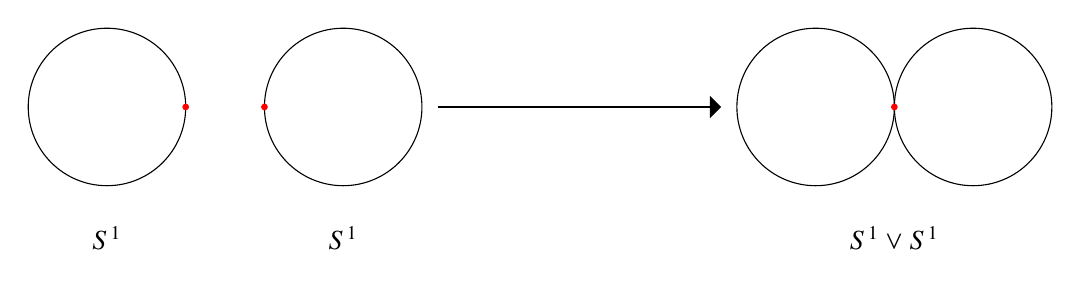
\begin{tikzpicture}[scale=1, >=triangle 90]
\begin {scope}
  \draw  (0,0) circle (1cm);
  \draw  (3,0) circle (1cm);
  \filldraw [red] (1,0) circle (1pt);
  \filldraw [red] (2,0) circle (1pt);
  \draw  (0,-1.4) node [anchor=north] {$S^1$};  
  \draw  (3,-1.4) node [anchor=north] {$S^1$};  
\end {scope}

\draw [->](4.2,0) -- (7.8,0);
 
\begin {scope}[xshift=9cm]
 \draw  (0,0) circle (1cm);
 \draw  (2,0) circle (1cm);
 \filldraw [red] (1,0) circle (1pt);
  \draw  (1,-1.4) node [anchor=north] {$S^1\vee S^1$};  
\end {scope}
\end{tikzpicture}

\caption{}
\end{figure}

  \item analog: $\R^2\setminus\{2 \text{Punkte}\}\cong \Z*\Z$
\begin{figure}[H]
 \centering
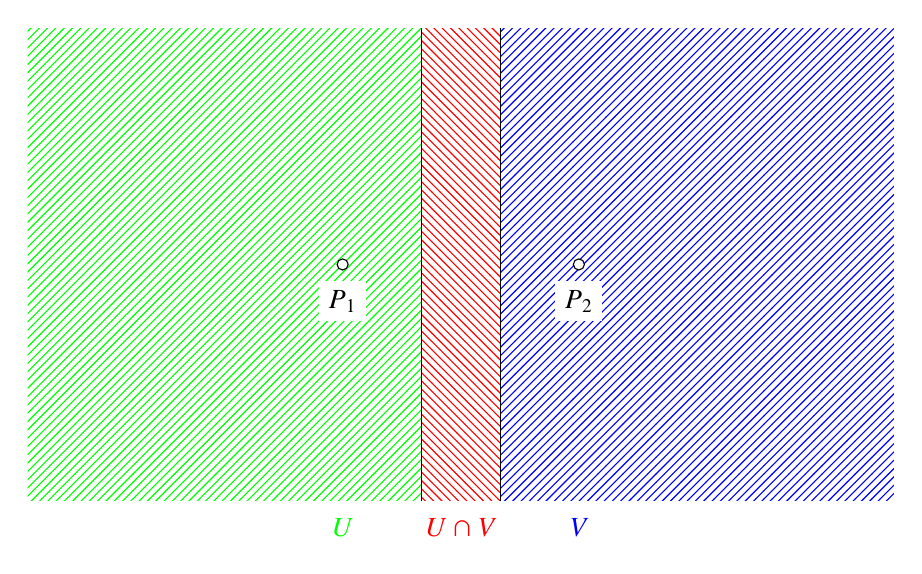
\begin{tikzpicture}[scale=1, >=triangle 90]
\begin {scope}
  \fill [pattern=north east lines,pattern color = green]  (1,3) -- (1,-3) -- (-4,-3) -- (-4,3) --cycle;
  \fill [pattern=north east lines,pattern color = blue]  (2,3) -- (2,-3) -- (7,-3) -- (7,3) --cycle;
  \fill [pattern=north west lines,pattern color = red]  (1,3) -- (1,-3) -- (2,-3) -- (2,3) --cycle;
  \draw [fill=white] (0,0) circle (2pt);
  \draw (1,-3) -- (1,3);
  \draw (2,-3) -- (2,3);
  \draw [fill=white] (3,0) circle (2pt);
  \draw  (0,-0.2) node [anchor=north,fill=white] {$P_1$}; 
  \draw  (3,-0.2) node [anchor=north,fill=white] {$P_2$};   
  \draw  (0,-3.1) node [anchor=north,green] {$U$}; 
  \draw  (1.5,-3.1) node [anchor=north,red] {$U\cap V$}; 
  \draw  (3,-3.1) node [anchor=north,blue] {$V$}; 
\end {scope}
\end{tikzpicture}


\caption{}
\end{figure}
 \end{enumerate}
\end{ex*}
Wir wollen nun Satz \ref{thm2:5.2} beweisen. Hierfür benötigen wir noch folgendes Lemma:
\begin{lem}\label{thm2:5.4}
 Sei $\phi:G\to H$ ein surjektiver Gruppenhomomorphismus. Dann ist die Abbildung $\bar \phi: G/\ker(\phi) \to H, \bar \phi(g\cdot \ker(\phi)):=\phi(g)$ wohldefiniert und ein Isomorphismus von Gruppen.
\end{lem}
\begin{proof}
 Da $\ker(\phi)\subset G$ ein Normalteiler ist, $G/\ker(\phi)$ eine Gruppe mit Verknüpfung
\[
 (g \cdot \ker(\phi))\cdot(k\cdot \ker(\phi)) = g \cdot k \cdot \ker(\phi)
\]
Also folgt die Homomorphieeigenschaft:
\[
 \bar \phi ((g \cdot \ker(\phi))\cdot(k\cdot \ker(\phi))) = \bar \phi (g \cdot k \cdot \ker(\phi)) = \phi (gk) = \phi (g) \phi (k) = \bar \phi (g \cdot \ker(\phi))  \bar \phi (k \cdot \ker(\phi))
\]

Die Abbildung $\bar \phi$ ist wohldefiniert, denn wenn $k\in \ker(\phi)$, denn ist $\phi(g\cdot k)=\phi(gk)=\phi(g)\cdot \phi(k)=\phi(g)$ und offensichtlich surjektiv. Sie ist injektiv, denn $\bar \phi(g\cdot \ker(\phi))=1$ impliziert $g\in \ker(\phi)$.
\end{proof}
Wir schreiben einen surjektiven Gruppenhomomorpohismus $\phi: \pi_1(U;x_0)*\pi_1(V;x_0)\to \pi_1(X;x_0)$ (und zeigen dann $N=\ker\phi$).

\emph{Wir definieren $\phi$ wie folgt.} Sei $[\omega_1]_{W_1}\cdot [\omega_2]_{W_2}\cdot ... [\omega_k]_{W_k}$ ein reduziertes Wort in $\pi_1(U; x_0)*\pi_1(V;x_0)$, dass heißt $W_i=U$ oder $V$ aber immer abwechselnd und $[\omega_i]\in \pi_1(W_i;x_0)$.

Sei $[\omega_1]_X\cdot [\omega_2]_X\cdot ... [\omega_k]_X$ das Bild dieses Wortes in $\pi_1(X;x_0)$. Diese Abbildung ist offensichtlich ein Gruppenhomorphismus.
\begin{lem} \label{thm2:5.5}
 $\phi$ ist surjektiv
\end{lem}
\begin{proof}
 Sei $\omega\in \Omega(X;x_0)$. Mit einem Kompaktheitsargument kann man zeigen, dass es eine Unterteilung des Intervalls $[0,1]$ gibt, dass heißt $0=t_0<t_1<\dotsb <t_{k-1}<t_k=1$, so dass $\omega([t_i, t_{i+1}])$, ganz in $U$ oder ganz in $V$ liegt.
\begin{figure}[H]
 \centering
\fixme[fig109]
\caption{}
\end{figure}
Durch Weglassen von Unterteilungspunkten erreichen wir, dass $U$ und $V$ sich abwechseln, insbesondere gilt dann $\omega(t_i)\in U\cap V$. Wähle Wege $\alpha_i:[0,1]\to U\cap V$ von $x_0$ nach $\omega(t_i).$

Dann ist $\omega_i:=\alpha_{i-1} * \omega|_{[t_{i-1}, t_i]}*\alpha_i^{-1}$ eine Schleife mit Basispunkt $x_0$, die ganz in $U$ bzw. ganz in $V$ liegt, wobei wir $\alpha_0$ und $\alpha_k$ als konstante Schleifen in $x_0$ wählen. Nun gilt:
\begin{align*}
 &[\omega_1]_X\cdot \dotso \cdot [\omega_k]_X=[\omega_1* \dotsm *\omega_k]_X\\
&=\left [\alpha_0*\omega|_{[t_0,t_1]}*\alpha_1^{-1}*\alpha_1*\omega|_{[t_1, t_2]}*\alpha_2^{-1}*\alpha_2 * \dotsm *\alpha_{k-1}^{-1}*\alpha_{k-1}*\omega|_{[t_{k-1},t_k]}*\alpha_k \right ]_X\\
&= [\omega|_{[t_0, t_1]}]* \dotsm *\omega|_{[t_{k-1}, t_k]}]_X=[\omega]_X.
\end{align*}
\end{proof}
\begin{lem}
 $N\subset \ker(\phi)$.
\end{lem}
\begin{proof}
 $N$ ist der von der Menge
\[
 \{[\omega]_U\cdot [\omega]_V^{-1}|\omega\in \Omega(U\cap V;x_0)\}\subset \pi_1(V;x_0)*\pi_1(V;x_0)\}
\]
erzeugte Normalteiler. Sei $\omega\in \Omega(U\cap V; x_0)$. Dann gilt $\phi([\omega]_U\cdot [\omega]_V^{-1})=[\omega]_X\cdot [\omega]_X^{-1}=1$, also liegen alle Elemente der obigen Menge im Kern, also auch der davon erzeugte Normalteiler.
\end{proof}
\begin{lem}\label{thm2:5.7}
 $\ker(\phi)\subset N$
\end{lem}
\begin{proof}
 Sei $\omega$ ein Wort $[\alpha_1]\cdot[\beta_1]\cdot[\alpha_2]\cdot[\beta_2]\cdot\dotsc\cdot[a_k]\cdot[\beta_k]$ mit $[\alpha_i]\in \pi_1(U;x_0)$, $[\beta_i]\in \pi_1(V;x_0)$. Sei $\omega\in \ker(\phi)$, dass heißt es gibt eine Homotopie 
$H:[0,1]\times[0,1]\to X$, $(s,t)\mapsto H(s,t)$ mit 
\[
 H(\cdot, 0)=\alpha_1*\beta_1*\dotsb *\alpha_k*\beta_k, H(\cdot, 1)=x_0
\]
\begin{figure}[H]
 \centering
\begin{tikzpicture}[scale=3, >=triangle 90]
\begin {scope}
  \draw (0,0) rectangle (1,1);
  \draw  (0,0) node [anchor=north east] {$0$}; 
  \draw  (1,0) node [anchor=north west] {$1$}; 
  \draw  (0,1) node [anchor=south east] {$1$};
  \draw  (0.5,0) node [anchor=north] {$\omega$};
  \draw  (0.5,1) node [anchor=south] {$x_0$};
  \draw  (0,0.5) node [anchor=east] {$x_0$};
  \draw  (1,0.5) node [anchor=west] {$x_0$};
\end {scope}
\draw [->] (1.2,0.5) -- (2.8,0.5);
\begin{scope}[xshift=3cm]
  \draw[step=.125cm] (0,0) grid (1,1);
  \draw  (0,0) node [anchor=north east] {$0$}; 
  \draw  (1,0) node [anchor=north west] {$1$}; 
  \draw  (0,1) node [anchor=south east] {$1$};
  \draw  (1,0.93) node [anchor=west,scale=1.1] {$\}\frac{1} {n}$};
  \draw  (1.05,1.05) node [anchor=south,scale=1.1,rotate=90] {$\}$};
  \draw  (0.93,1.05) node [anchor=south,scale=1.1] {$\frac{1} {n}$};
\end{scope}
\end{tikzpicture}

\caption{}
\end{figure}
Mit einem Kompaktheitsargument finden wir $n\in \N$, so dass die Teilquadrate von $[0,1]\times[0,1]$ der Seitenlänge $1/n$ ganz nach $U$ oder ganz nach $V$ abgebildet werden. Wir nehmen an, dass $n$ ein Vielfaches von $2k$ ist.

Die Beweisstragie ist nun, $\omega=H(\cdot, 0)$, in $x_0=H(\cdot, 1)$ schrittweise "`Zeile für Zeile"' überzuführen, wobei die in jedem Schritt verwendeten Wörter dieselbe Nebenklasse in $\pi_1(U;x_0)*\pi_1(V;x_0)/N$ repräsentieren:
\begin{figure}[H]
 \centering
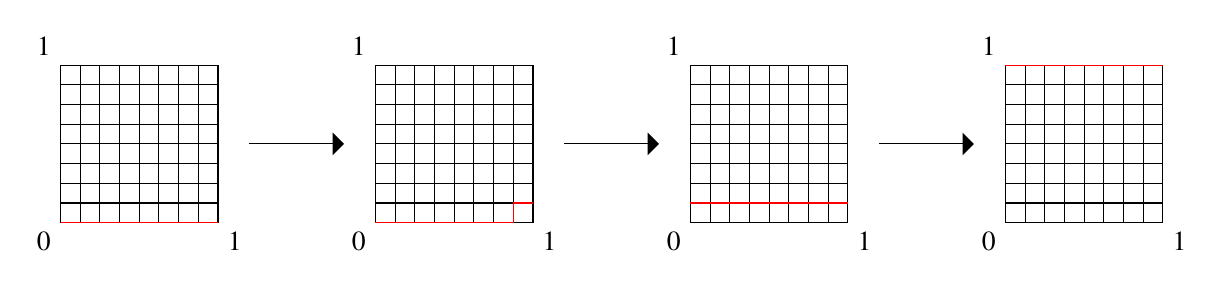
\begin{tikzpicture}[scale=2, >=triangle 90]
\begin{scope}[xshift=0cm]
  \draw[step=.125cm] (0,0) grid (1,1);
  \draw  (0,0) node [anchor=north east] {$0$}; 
  \draw  (1,0) node [anchor=north west] {$1$}; 
  \draw  (0,1) node [anchor=south east] {$1$};
  \draw [-,red] (0,0) -- (1,0);
\end{scope}
\draw [->] (1.2,0.5) -- (1.8,0.5);
\begin{scope}[xshift=2cm]
  \draw[step=.125cm] (0,0) grid (1,1);
  \draw  (0,0) node [anchor=north east] {$0$}; 
  \draw  (1,0) node [anchor=north west] {$1$}; 
  \draw  (0,1) node [anchor=south east] {$1$};
  \draw [-,red] (0,0) -- (0.875,0) -- (0.875,0.125) -- (1,0.125);
\end{scope}
\draw [->] (3.2,0.5) -- (3.8,0.5);
\begin{scope}[xshift=4cm]
  \draw[step=.125cm] (0,0) grid (1,1);
  \draw  (0,0) node [anchor=north east] {$0$}; 
  \draw  (1,0) node [anchor=north west] {$1$}; 
  \draw  (0,1) node [anchor=south east] {$1$};
  \draw [-,red] (0,0.125) -- (1,0.125);
\end{scope}
\draw [->] (5.2,0.5) -- (5.8,0.5);
\begin{scope}[xshift=6cm]
  \draw[step=.125cm] (0,0) grid (1,1);
  \draw  (0,0) node [anchor=north east] {$0$}; 
  \draw  (1,0) node [anchor=north west] {$1$}; 
  \draw  (0,1) node [anchor=south east] {$1$};
  \draw [-,red] (0,1) -- (1,1);
\end{scope}
\end{tikzpicture}

\caption{}
\end{figure} 
Wir benötigen folgende Vorbereitung.

Sei $f$ eine monoton steigende Funktion $[0,1]\to[0,1]$ die jeweils auf einer Umgebung von $k/n$ konstant ist.
\begin{figure}[H]
 \centering
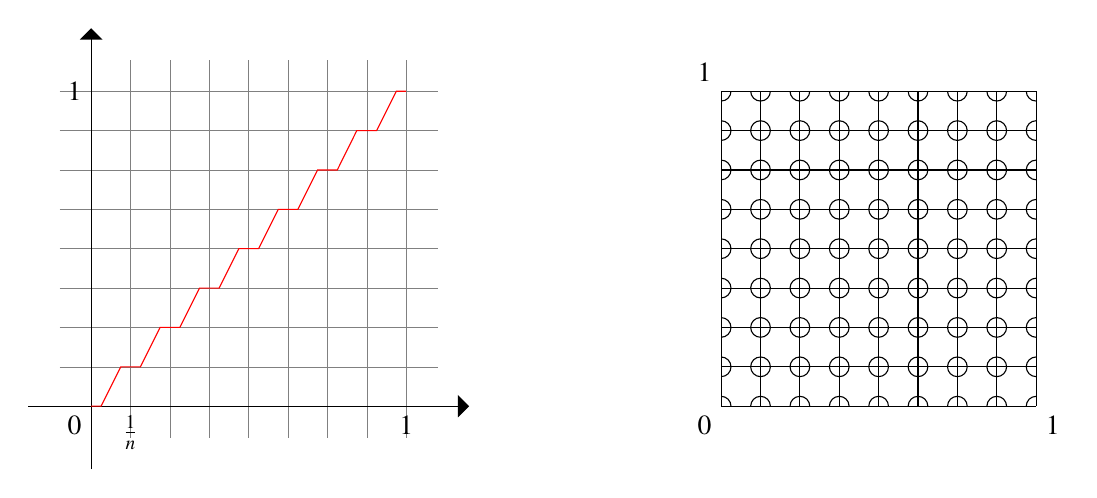
\begin{tikzpicture}[scale=4, >=triangle 90]
\begin{scope}[xshift=0cm]
  \draw[step=.125cm,gray,very thin] (-0.1,-0.1) grid (1.1,1.1);
  \draw [->] (0,-0.2) -- (0,1.2);
  \draw [->] (-0.2,0) -- (1.2,0);
  \draw  (0,0) node [anchor=north east] {$0$}; 
  \draw  (1,0) node [anchor=north] {$1$}; 
  \draw  (0,1) node [anchor=east] {$1$};
  \draw  (0.125,0) node [anchor=north] {$\frac{1}{n}$}; 
  \draw [-,red] (0,0) -- (0.03125,0) -- (0.09375,0.125) -- (0.15625,0.125) -- (0.21875,0.25) -- (0.28125,0.25) -- (0.34375,0.375) -- (0.40625,0.375) -- (0.46875,0.5) -- (0.53125,0.5) -- (0.59375,0.625) -- (0.65625,0.625) -- (0.71875,0.75) -- (0.78125, 0.75) -- (0.84325,0.875) -- (0.90625,0.875) -- (0.96875,1) -- (1,1);
\end{scope}

\begin{scope}[xshift=2cm]
 \draw[step=.125cm] (0,0) grid (1,1);
  \draw  (0,0) node [anchor=north east] {$0$}; 
  \draw  (1,0) node [anchor=north west] {$1$}; 
  \draw  (0,1) node [anchor=south east] {$1$};

\foreach \x in {1,...,7}
  \foreach \y in {1,...,7}
   { \draw (\x/8,\y/8) circle (0.03125cm);}

  \foreach \y in {1,...,7}
     { \draw (0,\y/8 -0.03125) arc (-90:90:0.03125cm);
       \draw (1,\y/8 +0.03125) arc (90:270:0.03125cm);
      }

  \foreach \x in {1,...,7}
     { \draw (\x/8 +0.03125,0) arc (0:180:0.03125cm);
	\draw (\x/8 -0.03125,1) arc (180:360:0.03125cm);
      }
  
  \draw (0.03125,0) arc (0:90:0.03125cm);
  \draw (0, 1-0.03125) arc (-90:0:0.03125cm);

  \draw (1,0.03125) arc (90:180:0.03125cm);
  \draw (1-0.03125,1) arc (180:270:0.03125cm);
\end{scope}
\end{tikzpicture}

\caption{}
\end{figure}
und ersetze $H$ durch $(t,s)\mapsto H(f(s), f(t))$. Dann ist $H$ auf einer Kreisschreibe um jeden Gitterpunkt konstant.  Wir erreichen, dass $H$ auf den Gitterpunkten den Wert $x_0$ annimmt (Wähle einen Weg nach $x_0$ und verwende den Radius der Kreisscheibe zum Umparametrisieren). Jetzt wird jede Kante im Gitter auf eine Schleife mit Basispunkt $x_0$ abgebildet.
\begin{figure}[H]
 \centering
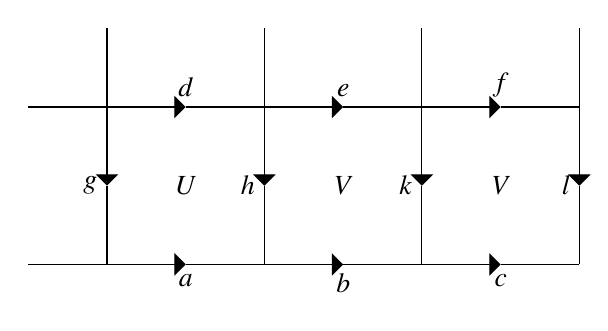
\begin{tikzpicture}[scale=2, >=triangle 90]
\begin{scope}[xshift=0cm]
 
  \draw  [->] (0,0) -- (1,0);
  \draw  [->] (1,0) -- (2,0);
  \draw  [->] (2,0) -- (3,0);
  \draw  [-] (3,0) -- (3.5,0);
 
  \draw  [->] (0,1) -- (1,1);
  \draw  [->] (1,1) -- (2,1);
  \draw  [->] (2,1) -- (3,1);
  \draw  [-] (3,1) -- (3.5,1);
 
  \draw  [->] (0.5,1.5) -- (0.5,0.5);
  \draw  [->] (1.5,1.5) -- (1.5,0.5);
  \draw  [->] (2.5,1.5) -- (2.5,0.5);
  \draw  [->] (3.5,1.5) -- (3.5,0.5);

  \draw  [-] (0.5,0.5) -- (0.5,0);
  \draw  [-] (1.5,0.5) -- (1.5,0);
  \draw  [-] (2.5,0.5) -- (2.5,0);
  \draw  [-] (3.5,0.5) -- (3.5,0);

  \draw  (1,0.5) node [] {$U$};
  \draw  (2,0.5) node [] {$V$};
  \draw  (3,0.5) node [] {$V$};

  \draw  (1,0) node [anchor=north] {$a$};
  \draw  (2,0) node [anchor=north] {$b$};
  \draw  (3,0) node [anchor=north] {$c$};

  \draw  (1,1) node [anchor=south] {$d$};
  \draw  (2,1) node [anchor=south] {$e$};
  \draw  (3,1) node [anchor=south] {$f$};

  \draw  (0.5,0.5) node [anchor=east] {$g$};
  \draw  (1.5,0.5) node [anchor=east] {$h$};
  \draw  (2.5,0.5) node [anchor=east] {$k$};
  \draw  (3.5,0.5) node [anchor=east] {$l$};
\end{scope}
\end{tikzpicture}


\caption{}
\end{figure} 
\end{proof}
\begin{ex*}
 \begin{figure}[H]
 \centering
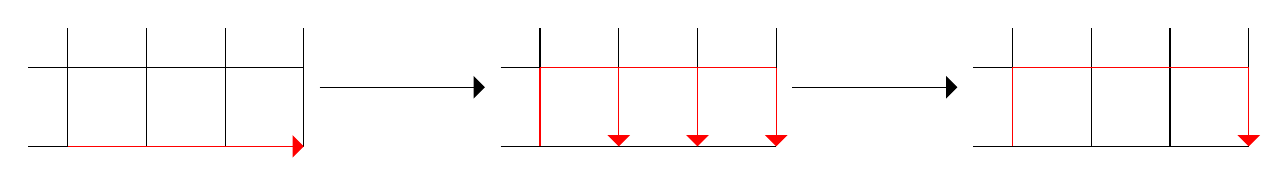
\begin{tikzpicture}[scale=1, >=triangle 90]
\begin{scope}[xshift=0cm]
  \draw  [-] (0,0) -- (3.5,0);
  \draw  [-] (0,1) -- (3.5,1);
 
  \draw  [-] (0.5,1.5) -- (0.5,0);
  \draw  [-] (1.5,1.5) -- (1.5,0);
  \draw  [-] (2.5,1.5) -- (2.5,0);
  \draw  [-] (3.5,1.5) -- (3.5,0);

  \draw  [->,red] (0.5,0) -- (3.5,0);
\end{scope}
\draw  [->] (3.7,0.75) -- (5.8,0.75);
\begin{scope}[xshift=6cm]
  \draw  [-] (0,0) -- (3.5,0);
  \draw  [-] (0,1) -- (3.5,1);
 
  \draw  [-] (0.5,1.5) -- (0.5,0);
  \draw  [-] (1.5,1.5) -- (1.5,0);
  \draw  [-] (2.5,1.5) -- (2.5,0);
  \draw  [-] (3.5,1.5) -- (3.5,0);
  
  \draw  [-,red] (0.5,0) -- (0.5,1);
  \draw  [-,red] (0.5,1) -- (3.5,1);
  \draw  [->,red] (1.5,1) -- (1.5,0);
  \draw  [->,red] (2.5,1) -- (2.5,0);
  \draw  [->,red] (3.5,1) -- (3.5,0);
\end{scope}
\draw  [->] (9.7,0.75) -- (11.8,0.75);
\begin{scope}[xshift=12cm] 
  \draw  [-] (0,0) -- (3.5,0);
  \draw  [-] (0,1) -- (3.5,1);
 
  \draw  [-] (0.5,1.5) -- (0.5,0);
  \draw  [-] (1.5,1.5) -- (1.5,0);
  \draw  [-] (2.5,1.5) -- (2.5,0);
  \draw  [-] (3.5,1.5) -- (3.5,0);

  \draw  [-,red] (0.5,0) -- (0.5,1);
  \draw  [-,red] (0.5,1) -- (3.5,1);
  \draw  [->,red] (3.5,1) -- (3.5,0);
\end{scope}
\end{tikzpicture}

\caption{}
\end{figure}
\begin{align*}
 [a]_U\cdot [b]_V\cdot [c]_V=[g^{-1}dh]_U\cdot [h^{-1} ek]_V\cdot [k^{-1}f l]_V=[g^{-1}d]_U\cdot \underbrace{[h]_U[h^{-1}]_V}_{\in N}\cdot [ekk^{-1}fl]_V\stackrel{\text{im Quotienten}}=[g^{-1}]_U[d]_U[e]_V\cdot [f]_V[l]_V 
\end{align*}
\end{ex*}

\section{Geometrische Anwendungen}
\subsection{Klassifikation der geschlossenen Flächen}
\begin{df}
 Eine \emph{geschlossene Fläche} ist eine $2-$dimensionale topologische Mannigfaltigkeit.

 \begin{figure}[H]
 \centering
\fixme[fig115]
\caption{}
\end{figure}
\end{df}

\begin{seg}{Ziel:}
Klassifikation bis auf Homöomorphie. Als Hilfsmittel werden wir sogenannte "`\emph{kombinatorische  Flächen}"' betrachten. (\textbf{Idee:} Triangulation von Flächen:)
 \begin{figure}[H]
 \centering
\fixme[fig116]
\caption{}
\end{figure}
\end{seg}
\begin{seg}{Vorbereitungen:}
 Seien $p_0, \dotsc  , p_m$ Vektoren im $\R^n$. Eine reelle Linearkombination:
\[
 \lambda_0p_0+\lambda_1p_1+\lambda_2p_2+\dotsb +\lambda_mp_m
\]
heißt \emph{Affinkombination}, falls $\lambda_1+\lambda_2+\dotsb +\lambda_m=1$ gilt, \emph{Konvexkombination}, falls zusätzlich $0\le \lambda_i\le 1$ für alle $i=0,\dotsc  , m$ gilt.

zum Beispiel:
 \begin{figure}[H]
 \centering
\fixme[fig117]
\caption{}
\end{figure}
Die Menge aller Affinkombinationen bzw. Konvexkombinationen von $p_0,\dotsc  , p_m$ wird mit $\operatorname{Aff}(p_0,\dotsc  ,p_m)$ bzw. $\operatorname{Kon}(p_0,\dotsc  ,p_m)$ bezeichnet.
 \begin{figure}[H]
 \centering
\fixme[fig118]
\caption{}
\end{figure}
$\operatorname{Kon}(p_0,\dotsc  .,p_m)$ heißt \emph{konvexe Hülle} von $p_0,\dotsc  ,p_m$. Eine Menge $\{p_0,\dotsc  ,p_m\}$ heißt \emph{affinunabhängig}, wenn $\dim(\operatorname{Aff}(p_0,\dotsc  ,p_m))=m$ ist.
\end{seg}
\begin{note*}
 $\operatorname{Aff}(p_0,\dotsc  , p_m)$ ist affiner Unterraum des $\R^n$
\end{note*}
\begin{exs*}
 \begin{enumerate}[(i)]
  \item \emph{Standardsimplex} $\Delta(e_1,.., e_{m+1})$ im $\R^{n+1}$
 \begin{figure}[H]
 \centering
\fixme[fig119]
\caption{ein Punkt (1) auf der Zahlengerade $\R$ (links); eine Strecke ($e_1e_2$) auf der Ebene $\R^2$ (zentral); Dreiecksfläche im Raum $\R^3$ rechts}
\end{figure} 
\item das $3$-Simplex $\Delta(0, e_1, e_2, e_3)$
 \begin{figure}[H]
 \centering
\fixme[fig120]
\caption{}
\end{figure}
 \end{enumerate}
\end{exs*}
\begin{df}
 Sei $\Sigma\subset \R^n$ ein $m$-dimensionaler Simplex mit Eckpunkten $p_0, \dotsc  , p_m$. 
Ein $r$-dimensionales \emph{Teilsimplex} ist eine Teilmenge $\Sigma'\subset \Sigma$ der Gestalt.
\[
 \Sigma'=\Delta(q_0,\dotsc  , q_r)
\]
wobei $\{q_0,\dotsc  , q_r\}\subset\{p_0,\dotsc  , p_m\}$

Der \emph{Rand} $\delta \Sigma$ ist die Vereinigung aller $(m-1)-$dimensionalen Teilsimplizes von $\Sigma$.
 \begin{figure}[H]
 \centering
\fixme[fig121]
\caption{}
\end{figure}
Man kann nun geometrische Körper im $\R^n$, als Vereinigung von Simplizes darstellen, dabei fordern wir, 
 \begin{figure}[H]
 \centering
\fixme[fig122]
\caption{}
\end{figure}[H]
dass sich je zwei beteiligte Simplizes nur im einem gemeinsamen Teilsimplex schneiden dürfen:
 \begin{figure}[H]
 \centering
\fixme[fig123]
\caption{}
\end{figure}
\end{df}
\begin{df}
 Ein \emph{endliches simpliziales Polyeder} $(K, \mathcal{K})$ besteht aus einem Teilraum $K\subset \R^N$ und einer endlichen Familie $\mathcal K=\bigcup \mathcal K_n$ von Teilmengen $\sigma\subset \R^N$, so dass gilt:
\begin{enumerate}[(i)]
 \item Jedes $\sigma\in \mathcal K_n$ ist eine $(n+1)-$elementige affin unabhängige Menge.
 \item Ist $\sigma \in \mathcal K$ und $\tau \subset \sigma$, dann ist auch $\tau \in \mathcal K$. Für $\sigma, \tau \in \mathcal K$, gilt $\Delta(\sigma)\cap \Delta(\tau)=\Delta(\sigma\cap\tau)$
 \item Es gilt $K=\bigcup_{\sigma\in \mathcal K}  \Delta(\sigma)$ 
\end{enumerate}

\end{df}
\begin{note*}
 \begin{enumerate}[(1)]
  \item $\mathcal K$ ist eine Familie von Eckenmengen, so dass die Eckenmenge von jedem Teilsimplex wieder in $\mathcal K$ enthalten sind. ($\mathcal K$ ist ein "`\emph{abstrakter simplizialer Komplex}"').
  \item $K$ ist die "'\emph{geometrische Realisierung}"'
  \item Nach (ii) gilt, dass sich zwei Simplizes nur in einem gemeinsamen Teilsimplex schneiden dürfen. (oder in der leeren Menge)
\end{enumerate}
\end{note*}
Nun zu den Flächen:
\begin{df}
 \emph{Eine kombinatorische  Fläche} ist endliches simpliziales Polyeder $(X, \mathcal X)$ mit folgenden Eigenschaften:
\begin{enumerate}[(i)]
 \item Jedes Simplex von $\mathcal X$ ist in einem $2-$Simplex von $\mathcal X$ enthalten.
 \item Jedes $1$-Simplex von $\mathcal X$ ist in höchstens zwei $2$-Simplizes enthalten.
 \begin{figure}[H]
 \centering
\fixme[fig124]
\caption{}
\end{figure}
 \item Ist $p$ ein $0$-Simplex in $\mathcal X$, so gibt es eine Anordnung $\Delta_1,\dotsc  ,\Delta_n$ der $2$-Simplizes
von $\mathcal X$, die $p$ enthalten, so dass $\Delta_i$ und $\Delta_{i+1}$ jeweils eine Seite gemeinsam haben.
 \begin{figure}[H]
 \centering
\fixme[fig125]
\caption{}
\end{figure}
(es kann sein dass auch $\Delta_n$ und $\Delta_1$ eine Seite gemeinsam haben, dann ist $p$ ein \emph{innerer Punkt}, andernfalls ein \emph{Randpunkt}.
\end{enumerate}
\end{df}
\begin{exs*}[kombinatorische Fläche] 
\begin{figure}[H]
 \centering
\fixme[fig126]
\caption{}
\end{figure}
auch: "'\emph{Zerschneidung}"' daran, kombinatorische Fläche mit Rand
 \begin{figure}[H]
 \centering
\fixme[fig127]
\caption{}
\end{figure}
kombinatorische "`Brezelfläche"':
 \begin{figure}[H]
 \centering
\fixme[fig128]
\caption{}
\end{figure}
\end{exs*}
\begin{st}[Rado 1924]
 Jede geschlossene Fläche tritt als geometrische Realisierung $K$ ist homöomorph zu einer kombinatorische Fläche ($K, \mathcal K)$ auf (ist "'\emph{triangulierbar}"'))
\end{st}

\begin{df}
 Sind $(K, \mathcal K)$, $(L, \mathcal L)$ zwei endliche simpliziale Polyeder, so heißt eine stetige Abbildung $f: K \to L$ \emph{simplizial}, wenn für jedes $\sigma\in \mathcal K$
\begin{enumerate}[(i)]
 \item die Bildmenge $f(\sigma)$ ein Element von $\mathcal L$ ist.
 \item die Abbildung $f\vline\,_{\Delta(\sigma)}: \Delta(\sigma)\to \Delta(f(\sigma))$ affin ist.
\end{enumerate}

Die Abbildung heißt \emph{Isomorphismus}, wenn sie eine simpliziale Umkehrabbildung hat.
\end{df}
\begin{df}
 Zwei kombinatorische Flächen heißen \emph{kombinatorisch äquivalent}, wenn sie isomorphe "`\emph{Unterteilungen}"' besitzen.
\end{df}
\begin{figure}[H]
 \centering
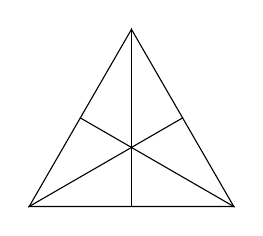
\begin{tikzpicture}[scale=3, >=triangle 90]
\node [regular polygon, regular polygon sides = 3,draw,name=dreieck,minimum size = 3cm] at (0,0) {};
\draw [-](dreieck.corner 3) -- (dreieck.side 1);
\draw [-](dreieck.corner 1) -- (dreieck.side 2);
\draw [-](dreieck.corner 2) -- (dreieck.side 3);
\end{tikzpicture}


\caption{Unterteilung}
\end{figure}

\begin{df}
 Eine \emph{Zerschneidung} einer kombinatorischen Fläche  $(X, \mathcal X)$ besteht aus einer kombinatorischen Fläche $(Y,\mathcal Y)$ und einer simplizialen Abbildung. $\phi:(Y, \mathcal Y)\to (X, \mathcal X)$, so dass $\phi\vline\,_{\mathcal Y_2}:\mathcal Y_2 \to \mathcal X_2$ bijektiv ist. (bijektiv auf 2 Simplizes, $0$- und $1$-Simplizes werden eventuell zusammengeklebt.)
\begin{figure}[H]
 \centering
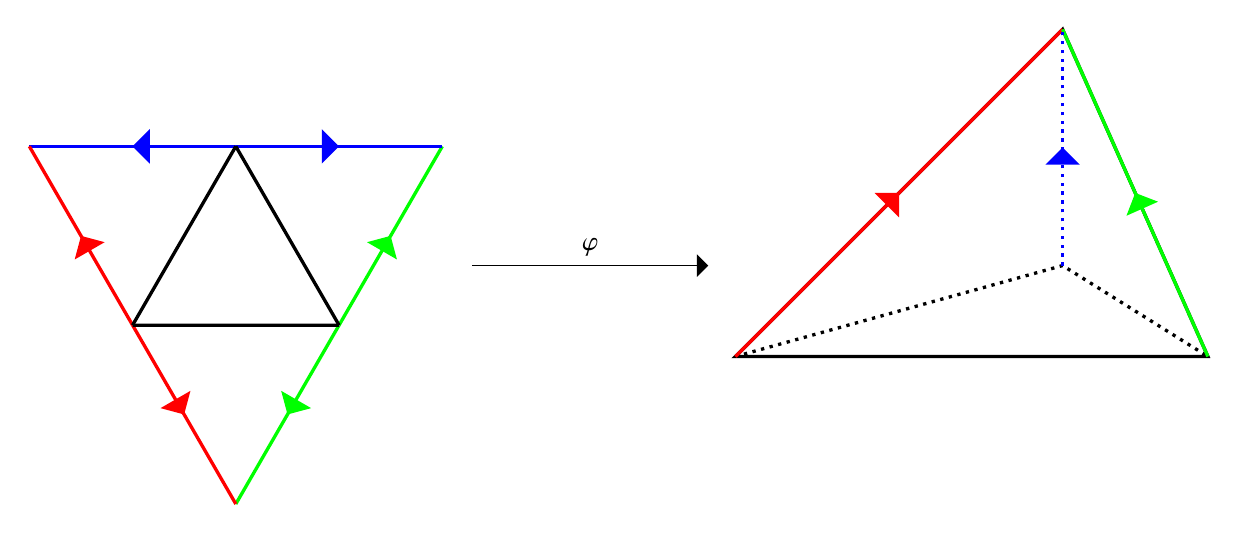
\begin{tikzpicture}[scale=3, >=triangle 90]
\node [regular polygon, regular polygon sides = 3,name=dreieck,minimum size = 3cm,rotate=180,scale=2] at (0,0) {};
\begin{scope}[very thick,decoration={
    markings,
    mark=at position 0.5 with {\arrow{>}}}
    ] 
    \draw[postaction={decorate},green] (dreieck.side 1) -- (dreieck.corner 1);
    \draw[postaction={decorate},green] (dreieck.side 1) -- (dreieck.corner 2);
    \draw[postaction={decorate},blue] (dreieck.side 2) -- (dreieck.corner 2);
    \draw[postaction={decorate},blue] (dreieck.side 2) -- (dreieck.corner 3);
    \draw[postaction={decorate},red] (dreieck.side 3) -- (dreieck.corner 3);
    \draw[postaction={decorate},red] (dreieck.side 3) -- (dreieck.corner 1);
    \draw [-](dreieck.side 1) -- (dreieck.side 2);
    \draw [-](dreieck.side 2) -- (dreieck.side 3);
    \draw [-](dreieck.side 3) -- (dreieck.side 1);
\end{scope}
\draw  [->] (1,0) --  node [above] {$\varphi$} (2,0);
\begin{scope}[very thick,xshift=3.5cm,decoration={
    markings,
    mark=at position 0.5 with {\arrow{>}}}
    ] 

    \draw (-1,0,1) -- (1,0,1) -- (0,1,0) -- cycle;
    \draw[dotted](-1,0,1) -- (0,0,0) -- (1,0,1);
    \draw[dotted](0,0,0) -- (0,1,0);
    \draw[postaction={decorate},red] (-1,0,1) -- (0,1,0) ;
    \draw[postaction={decorate},green] (1,0,1) -- (0,1,0) ;
    \draw[postaction={decorate},dotted,blue] (0,0,0) -- (0,1,0) ;
  
\end{scope}
\end{tikzpicture}

\caption{}
\end{figure}
\end{df}

Statt Zerschneidung betrachten wir später einen etwas allgemeineren Begriff (Polygonmodell)
\begin{seg}{Zerschneidung eines $2$-Torus}
 \begin{figure}[H]
 \centering
\fixme[fig131]
\caption{}
\end{figure}
\end{seg}

\begin{df}
 Der \emph{Rand} einer kombinatorischen Fläche besteht aus allen $1$-Simplizes, die nicht Teilsimplizes in zwei verschiedenen $2$-Simplizes sind. Eine kombinatorische Fläche heißt \emph{n-Eck}, wenn ihr Rand aus genau n $1$-Simplizes besteht und sie zu einem $2$-Simplex homöomorph ist.
\begin{figure}[H]
 \centering
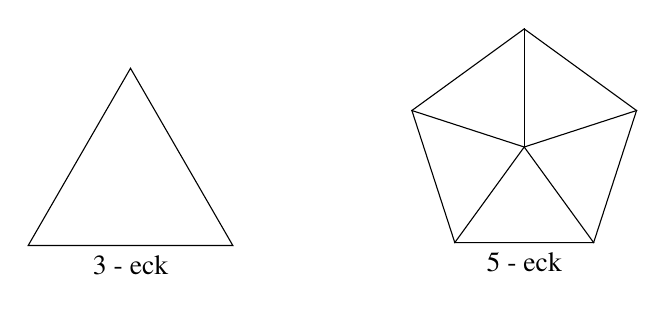
\begin{tikzpicture}[scale=1, >=triangle 90]
\begin{scope}
  \node [regular polygon, regular polygon sides = 3,minimum size = 3cm,name=dreieck,draw] at (0,0) {};
  \node [below] at (dreieck.south)  {3 - eck};  
\end{scope}
\begin{scope}[xshift=5cm,yshift=0.5cm]
  \node [regular polygon, regular polygon sides = 5,minimum size = 3cm,name=fuenfeck,draw] at (0,0) {};
  \draw [-](fuenfeck.corner 1) -- (fuenfeck.center);
  \draw [-](fuenfeck.corner 2) -- (fuenfeck.center);
  \draw [-](fuenfeck.corner 3) -- (fuenfeck.center);
  \draw [-](fuenfeck.corner 4) -- (fuenfeck.center);
  \draw [-](fuenfeck.corner 5) -- (fuenfeck.center);
  \node [below] at (fuenfeck.south)  {5 - eck};  
\end{scope}
\end{tikzpicture}


\caption{}
\end{figure}
\end{df}

\begin{lem}\label{thm3:1.11} 
 Sei $\phi: \mathcal Y\to \mathcal X$ eine Zerschneidung von $\mathcal X$ \emph{entlang eines $1$-Simplex} $e$ (dass heißt $\phi^{-1}(e)$ besteht aus zwei $1-$Simplizes von $\mathcal Y$, alle anderen haben nur ein $1$-Simplex im Urbild. Sei $\mathcal Y$ die disjunkte Vereinigung eines $n$-Ecks und eines $m$-Ecks. Dann ist $\mathcal X$ ein ($m+n-2$)-Eck.
\end{lem}
\begin{proof}
.
 \begin{figure}[H]
 \centering
\begin{tikzpicture}[scale=1, >=triangle 90]
\begin{scope}
  \node [regular polygon, regular polygon sides = 6,minimum size = 3cm,name=6eck,rotate=90] at (0,0) {};
  \draw [-](6eck.corner 1) -- (6eck.corner 2);
  \draw [-](6eck.corner 2) -- (6eck.corner 3);
  \draw [-](6eck.corner 3) -- (6eck.corner 4);
  \draw [-,red](6eck.corner 4) -- (6eck.corner 5);
  \draw [-](6eck.corner 5) -- (6eck.corner 6);
  \draw [-](6eck.corner 6) -- (6eck.corner 1);
\end{scope}
\begin{scope}[xshift=2.8cm,yshift=0cm]
  \node [regular polygon, regular polygon sides = 5,minimum size = 3cm,name=5eck,rotate=-90,scale=5/6] at (0,0) {};
  \draw [-](5eck.corner 1) -- (5eck.corner 2);
  \draw [-](5eck.corner 2) -- (5eck.corner 3);
  \draw [-,red](5eck.corner 3) -- (5eck.corner 4);
  \draw [-](5eck.corner 4) -- (5eck.corner 5);
  \draw [-](5eck.corner 5) -- (5eck.corner 1);  
\end{scope}

\draw [->] (4.5,0) -- node [above] {$\varphi$}(6,0);
\begin{scope}[xshift=8cm]
\begin{scope}
  \node [regular polygon, regular polygon sides = 6,minimum size = 3cm,name=6eck,rotate=90] at (0,0) {};
  \draw [-](6eck.corner 1) -- (6eck.corner 2);
  \draw [-](6eck.corner 2) -- (6eck.corner 3);
  \draw [-](6eck.corner 3) -- (6eck.corner 4);
  \draw [-](6eck.corner 5) -- (6eck.corner 6);
  \draw [-](6eck.corner 6) -- (6eck.corner 1);
\end{scope}
\begin{scope}[xshift=2.3cm,yshift=0cm]
  \node [regular polygon, regular polygon sides = 5,minimum size = 3cm,name=5eck,rotate=-90,scale=5/6] at (0,0) {};
  \draw [-](5eck.corner 1) -- (5eck.corner 2);
  \draw [-](5eck.corner 2) -- (5eck.corner 3);
  \draw [-](5eck.corner 4) -- (5eck.corner 5);
  \draw [-](5eck.corner 5) -- (5eck.corner 1);
\end{scope}
\end{scope}
\end{tikzpicture}

\caption{}
\end{figure}
\end{proof}
\begin{st}
 Eine zusammenhängende kombinatorische Fläche lässt sich zu einem $m$-Eck zerschneiden.
\end{st}
\fixme[from mathematiker : Überprüfe Nummerierung]
\begin{proof}
 Eine Zerschneidung $\mathcal Y$ von $\mathcal X$ heißt \emph{flach}, wenn jede Komponente $\mathcal Y_i$ von $\mathcal Y$ ein $n_i$-Eck ist. Es existiert immer eine flache Zerschneidung, zum Beispiel die disjunkte Vereinigung der $2$-Simplizes von $\mathcal X$.
\begin{figure}[H]
 \centering
\fixme[fig134]
\caption{}
\end{figure}
Sei unter all solchen eine mit minimaler Anzahl von Komponenten gewählt.
Diese Anzahl ist gleich 1:
 Da $\mathcal X$ zusammenhängend ist, gibt es nämlich sonst zwei $1$-Simplizes in $\mathcal Y$, die von $\phi$ identifiziert werden. Nach Lemma \ref{thm3:1.11} lassen sich diese zu einem $n$-Eck zusammenkleben, wobei eine neue flache Zerschneidung mit verringerter Komponentenzahl entsteht.
\end{proof}

Eine Zerschneidung $\phi: \mathcal Y \to \mathcal X$ einer geschlossenen Fläche liefert eine Äquivalenzrelation auf dem Rand von $\mathcal Y$: Jede Randkante wird mit genau einer anderen verklebt. Für diese Identifikation gibt es genau zwei Möglichkeiten, die den beiden Möglichkeiten entsprechen, die Menge der Endpunkte $\{p_0, p_1\}$ eines $1$-Simplex $\Delta(p_0, p_1)$ auf die Menge der Endpunkte $\{a_0, a_1\}$ eines anderen $1$-Simplex bijektiv abzubilden.

Sei $\mathcal k=\{a_1, \dotsc  , a_{2n}\}$ die Menge der Kanten von $\mathcal Y$. Wir geben den Kanten eine Orientierung, indem wir fordern, dass beim positiven Durchlaufen das Innere von $\mathcal Y$ links liegen soll.

\begin{figure}[H]
 \centering
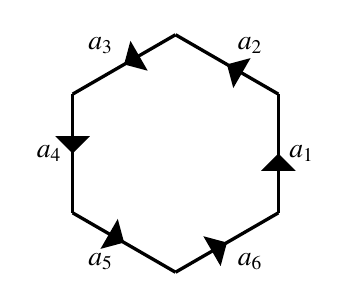
\begin{tikzpicture}[scale=1, >=triangle 90]
\node [regular polygon, regular polygon sides = 6,minimum size = 3cm,name=6eck,rotate=90] at (0,0) {};
\begin{scope}[very thick,decoration={
    markings,
    mark=at position 0.5 with {\arrow{>}}}
    ] 
  
  \draw [postaction={decorate}](6eck.corner 1) -- (6eck.corner 2);
  \draw [postaction={decorate}](6eck.corner 2) -- (6eck.corner 3);
  \draw [postaction={decorate}](6eck.corner 3) -- (6eck.corner 4);
  \draw [postaction={decorate}](6eck.corner 4) -- (6eck.corner 5);
  \draw [postaction={decorate}](6eck.corner 5) -- (6eck.corner 6);
  \draw [postaction={decorate}](6eck.corner 6) -- (6eck.corner 1);
  \node [left] at (6eck.side 1)  {$a_4$};  
  \node [below left] at (6eck.side 2)  {$a_5$};  
  \node [below right] at (6eck.side 3)  {$a_6$};  
  \node [right] at (6eck.side 4)  {$a_1$};  
  \node [above right] at (6eck.side 5)  {$a_2$};  
  \node [above left] at (6eck.side 6)  {$a_3$};  
\end{scope}
\end{tikzpicture}


\caption{}
\end{figure}

Wir schreiben $a_i^{-1}$ für die jeweils umgekehrt durchlaufene Kante. Wir setzen $\mathcal k^0:=\{a_1,\dotsc, a_{2n}, a_1^{-1},\dotsc , a_{2n}^{-1}\}$ für die Menge der \emph{orientierten Kanten}.

\begin{df}
 Ein \emph{Polygon-Modell} besteht aus einem $2n$-Eck $\mathcal Y$ mit Kantenmenge $\mathcal k$ und einer \emph{Involution} $\psi: \mathcal k^0 \to \mathcal k^0$, die folgende Bedingung erfüllt: Sind $a,b\in \mathcal k$ und ist $\psi(a)=b^{\epsilon}$, so ist $b\neq a$ und $\psi(a^{-1})=b^{-\epsilon}$.
\end{df}
\begin{note*}
 \emph{Involution} bedeutet $\psi\circ \psi=\id$
\end{note*}


\begin{exs*}
 \begin{enumerate}[(i)]
  \item \emph{Torus}:
\begin{figure}[H]
 \centering
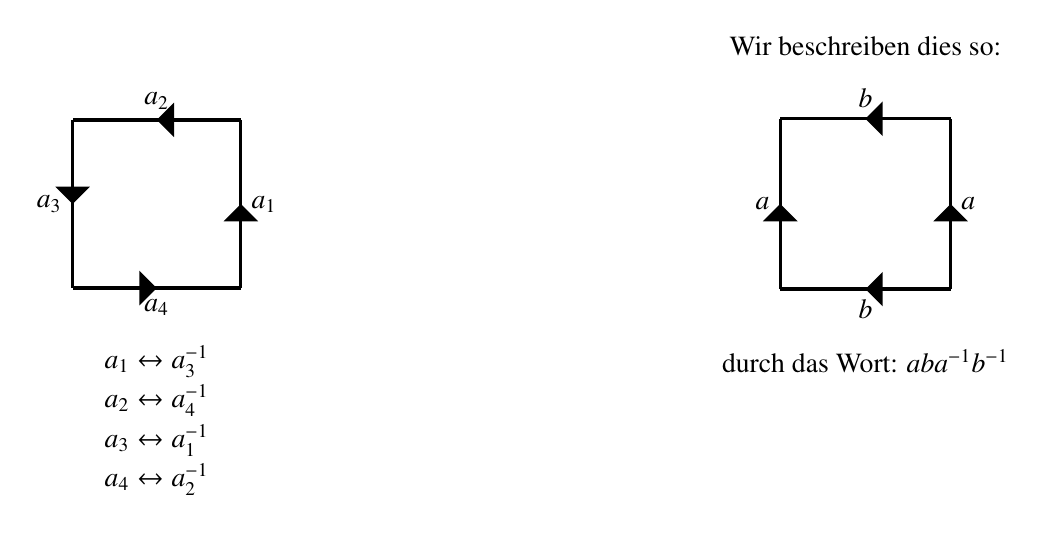
\begin{tikzpicture}[scale=1, >=triangle 90]
\node [regular polygon, regular polygon sides = 4,minimum size = 3cm,name=4eck] at (0,0) {};
\begin{scope}[very thick,decoration={
    markings,
    mark=at position 0.5 with {\arrow{>}}}
    ] 
  
  \draw [postaction={decorate}](4eck.corner 1) -- (4eck.corner 2);
  \draw [postaction={decorate}](4eck.corner 2) -- (4eck.corner 3);
  \draw [postaction={decorate}](4eck.corner 3) -- (4eck.corner 4);
  \draw [postaction={decorate}](4eck.corner 4) -- (4eck.corner 1);
 
  \node [right] at (4eck.side 4)  {$a_1$};  
  \node [above] at (4eck.side 1)  {$a_2$};  
  \node [left] at (4eck.side 2)  {$a_3$};  
  \node [below] at (4eck.side 3)  {$a_4$}; 
  \node at (0,-2)  {$a_1 \leftrightarrow a_3^{-1}$ }; 
  \node at (0,-2.5)  {$a_2 \leftrightarrow a_4^{-1}$ };
  \node at (0,-3)  {$a_3 \leftrightarrow a_1^{-1}$};
  \node at (0,-3.5)  {$a_4 \leftrightarrow a_2^{-1}$ }; 
\end{scope}

\begin{scope}[very thick,xshift=9cm,decoration={
    markings,
    mark=at position 0.5 with {\arrow{>}}}
    ] 
  \node [regular polygon, regular polygon sides = 4,minimum size = 3cm,name=4eck2] at (0,0) {};
 \node at (0,2)  {Wir beschreiben dies so:}; 
\node at (0,-2)  {durch das Wort: $aba^{-1}b^{-1}$}; 
  \draw [postaction={decorate}](4eck2.corner 1) -- (4eck2.corner 2);
  \draw [postaction={decorate}](4eck2.corner 3) -- (4eck2.corner 2);
  \draw [postaction={decorate}](4eck2.corner 4) -- (4eck2.corner 3);
  \draw [postaction={decorate}](4eck2.corner 4) -- (4eck2.corner 1);
 
  \node [right] at (4eck2.side 4)  {$a$};  
  \node [above] at (4eck2.side 1)  {$b$};  
  \node [left] at (4eck2.side 2)  {$a$};  
  \node [below] at (4eck2.side 3)  {$b$};  
\end{scope}
\end{tikzpicture}


\caption{}
\end{figure}
\item komplexeres Beispiel:
\begin{figure}[H]
 \centering
\fixme[fig137]
\caption{}
\end{figure}
Es ergibt sich das \emph{Wort}: $acfbf^{-1}db^{-1}d^{-1}ea^{-1}e^{-1}c^{-1}$
 \end{enumerate}
\end{exs*}
\begin{df}
 Ein \emph{Flächen-Wort} ist ein formaler Ausdruck
\[
 a_{i_1}^{\epsilon_1} a_{i_2}^{\epsilon_2} \dotsb a_{i_{2r}}^{\epsilon_{2r}}
\]
wobei $\epsilon_l=\pm 1$ und jeder Index $i\in \{1,\dotsc, r\}$ unter den Indizes $i_1, i_2, \dotsc , i_{2r}$ genau zweimal vorkommt. Das zugehörige Polygonmodell besteht aus einem $2r$-Eck mit zyklisch angeordneten Kanten $b_1,\dotsc , b_{2r}$ mit
\[
 \psi(b_\mu)=b_v^\epsilon \text{ für } i_\mu=i_v \text{ und } \epsilon_\mu=\epsilon \epsilon_v
\]
Zwei Flächen-Worte heißen äquivalent, wenn die durch sie beschriebenen Flächen kombinatorisch äquivalent sind.
(Auf die Triangulierung des Polygonmodells kommt es nicht an, S. E, Ossa 106.)
\end{df}
\begin{seg}{Ziel:}
 Klassifiziere Flächen-Worte bis auf Äquivalenz
\end{seg}
\begin{exs*}
\begin{enumerate}[(i)]
 \item \emph{Torus}: $aba^{-1}b^{-1}$ (äquivalent: $b^{-1}aba^{-1}$ oder zum Beispiel $a^{-1} b^{-1} a b$).
 \item \emph{Kleinsche Flasche}: $aba^{-1}b^{-1}$.
\begin{figure}[H]
 \centering
\fixme[fig138]
\caption{}
\end{figure}
\end{enumerate}
\end{exs*}
\begin{lem}
\begin{enumerate}
 \item Zyklische Vertauschung
 \item $\dotsb a^{\epsilon}\dotsb a^{\epsilon'}\dotsb \sim \dotsb a^{-\epsilon}\dotsb a^{-\epsilon'}\dotsb$
 \item $\dotsb ab\dotsb ab\dotsb \sim \dotsb a \dotsb a\dotsb$
 \item $\dotsb ab\dotsb b^{-1} a^{-1}\dotsb \sim \dotsb a \dotsb a^{-1} \dotsb$
\setcounter{figure}{139}
\begin{figure}[H]
 \centering
\fixme[fig140]
\caption{}
\end{figure}

\end{enumerate}
\end{lem}
\begin{proof}
 Offensichtlich.
\end{proof}
Man kann zum Beispiel immer erreichen, dass das erste Auftreten eines Buchstaben mit Exponent $+1$ ist (nach ii)
\begin{lem}[Beiziehen]
 \[
  \dotsb abb^{-1}c\dotsb  \sim \dotsb ac\dotsb 
 \]
\end{lem}
\begin{proof}
.
 \begin{figure}[H]
 \centering
\fixme[fig141]
\caption{}
\end{figure}
\end{proof}

Ein Flächen-Wort heißt \emph{gekürzt}, wenn kein $bb^{-1}$ (oder $b^{-1}b$) noch vorkommt. Wir wollen Flächen-Worte als gekürzt, außer sie sind von der Form $aa^{-1}$, wir wollen dies als Polygon-Modell der Sphäre zulassen.

\begin{note*}[Polygonmodelle mit 2 Kanten]
.
 \begin{figure}[H]
 \centering
\fixme[fig142]
\caption{}
\end{figure}
\end{note*}

\begin{note*}[Moebius-Band]
.
 \begin{figure}[H]
 \centering
\fixme[fig143]
\caption{}
\end{figure}
$\dotsb c\dotsb c\dotsb $ auch \emph{Kreuzhaube} genannt.
\end{note*}

\begin{note*}[Henkel]
$\dotsb a\dotsb b\dotsb a^{-1}\dotsb b^{-1}\dotsb $
 \begin{figure}[H]
 \centering
\fixme[fig144]
\caption{}
\end{figure}
\end{note*}
Die Anzahl der Äquivalenzklassen von Endpunkten von Kanten heißt \emph{Eckenzahl}
\begin{figure}[H]
 \centering
\fixme[fig145]
\caption{}
\end{figure}

besitzt Eckenzahl 1.

\begin{lem}\label{thm3:1.19}
 Ein gekürztes Flächen-Wort ist äquivalent zu einem gekürzten Flächenwort mit Eckenzahl 1
\end{lem}
\begin{ex*}
.
 \begin{figure}[H]
 \centering
\fixme[fig146]
\caption{}
\end{figure}
\end{ex*}
\begin{proof}
 Die Ecke $P$ kommt nun in verringerter Anzahl vor ($Q$ dafür einmal öfter). Durch Wiederholen erreicht man, dass $P$ nur noch einmal vorkommt. Dann haben wir entweder $aa^{-1}$ (fertig) oder $aa^{-1}\dotsb $ und wir können "`Beiziehen"'.
\end{proof}

\begin{lem}[Kreuzhauben-Normierung] \label{thm3: 1.18} 
 Ein gekürztes Flächen-Wort mit Eckenzahl $1$ und $k$ Kreuzhauben ist äquivalent zu einem Wort der Gestalt $c_1c_1\dotsb c_2c_2\dotsb c_kc_k\dotsb $, wobei alle sonstigen Kanten genau einmal mit Exponent $+1$ und einmal mit $-1$ auftreten.
\end{lem}
\begin{proof}
.
 \begin{figure}[H]
 \centering
\fixme[fig147]
\caption{}
\end{figure}
Bereits vorhandene Kreuzhauben der Form $dd$ werden dabei nicht verändert.
\end{proof}

\begin{lem}[Henkel-Normierung]
 Ein gekürztes Flächen-Wort mit Eckenzahl $1$ ist äquivalent zu einem Produkt von Worten der Gestalt $c_ic_i$ und $a_jb_ja_j^{-1}b_j^{-1}$
\end{lem}
\begin{proof}
 Wir nehmen an, dass die Kreuzhauben bereits normiert wie in Lemma \ref{thm3: 1.18} vorkommen. Dann muss das Wort von der Form $\dotsb a\dotsb b\dotsb a^{-1}\dotsb b^{\pm1}\dotsb $, denn sonst würde der Rand des Polygons, wenn man $a$ und $a^{-1}$ entfernt (nach Identifikation der übrigen entsprechenden Kanten) in zwei Komponenten zerfallen,
\begin{figure}[H]
 \centering
\fixme[fig148]
\caption{}
\end{figure}
Widerspruch zu Eckenzahl $1$. Der Exponent von $b^{\pm 1}$ muss $-1$ sein, wegen der vorherigen Kreuzhauben-Normierung. Wir formen nun $\dotsb a\dotsb b\dotsb a^{-1}\dotsb b^{-1}\dotsb $ zu $\dotsb aba^{-1}b^{-1}\dotsb $
\begin{figure}[H]
 \centering
\fixme[fig149]
\caption{}
\end{figure}
Bereits norimerte andere Henkel und normierte Kreuzhauben bleiben dabei normiert.
\end{proof}
\begin{lem}[Henkel-Elimination]
 Ein gekürztes Flächenwort mit Eckenzahl $1$, dass mindestens eine Kreuzhaube enthält, ist äquivalent zu einem Wort der Gestalt $c_1c_1c_2c_2\dotsb c_kc_k$
(einem Produkt von normierten Kreuzhauben).
\end{lem}
\begin{proof}
 Falls außer einer Kreuzhaube noch mindestens ein Henkel vorkommt, ist das Wort äquivalent zu $\dotsb ccaba^{-1}b^{-1}\dotsb $ Wir formulieren:
\begin{figure}[H]
 \centering
\fixme[fig150]
\caption{}
\end{figure}
Nun haben wir einen Henkel weniger und zwei Kreuzhauben mehr. (diese können normiert werden).
\end{proof}

\begin{note*}[Endergebnis]
 Wir können das Flächenwort äquivalent in eine der drei folgenden Normalformen umformen;
 \begin{enumerate}[(1)]
  \item $aa^{-1}$ die Realisierung dieses Worts  (die Sphäre) nennen wir auch $F_0$
  \item $a_1b_1a_1^{-1} b_1^{-1} a_2 b_2a_2^{-1} b_2^{-1}\dotsb a_gb_g a_g^{-1} b_g^{-1}$ die Realisierung nennen wir auch $F_g, g\ge 1$
  \item $c_1c_1c_2c_2\dotsb c_g$ die Realisierung nennen wir auch $N_g$.
 \end{enumerate}
Die Fläche $F_g, g\ge 0$ nennt man die \emph{orientierbaren geschlossenen Flächen von Geschlecht} $g$.
\begin{figure}[H]
 \centering
\fixme[fig151]
\caption{}
\end{figure}
Die Flächen $N_g, g\ge 1$ nennt man die \emph{nicht-orientierbaren Flächen} vom Geschlecht $g$
\begin{figure}[H]
 \centering
\fixme[fig152]
\caption{}
\end{figure}
\end{note*}
\begin{st}
 Jede geschlossene Fläche ist zu einem $F_g, g\ge 0$ oder $Ng, g\ge 1$ homöomorph. Wir haben noch nicht ausgeschlossen, dass die $F_g$ und $N_g$ untereinander homöomorph sind.
\end{st}
\begin{st}
 Sei $\omega(a_1,\dotsc  ,a_n)=a^{\epsilon_1}_{i_1} a^{\epsilon_2}_{i_2}\dotsb  a^{\epsilon_2r}_{i_{2r}}$ ein Flächenwort mit Eckenzahl $1$. Sei $X$ die Realisierung des zugehörigen Polygon-Modells und $x_0\in X$ das gemeinsame Bild der Endpunkte aller Kanten, dann hat $\pi_1(X;x_0)$ die Präsentation
\[
 \pi_1(X;x_0)=\langle a_1,\dotsc,a_r \, \vline \, w(a_1,\dotsc  ,a_r)=1\rangle
\]
dass heißt die freie Gruppe über $a_1,\dotsc  , a_r$ modulo dem von $w(a_1,\dotsc, a_r)$ erzeugten Normalteiler.
\begin{kor*}
 $\pi_1(F_g)_{ab}\cong \Z^g$, $\pi_1(N_g)_{ab}\cong \Z^{g-1} \oplus \Z_2$ abelsch gemachte Gruppe
\end{kor*}
\end{st}



\end{document}
